%&latex
% UF Sample ETD Main Document Fall 2014
% Documenting the dvipdfmx/dvipdfm "File not Found" error
% Improved method of handling the single/multiple appendices issue
% Updated font calls to meet latest LaTeX standards

% Define Document Class to be used and options - Choose the option that meets your OS%
\documentclass[12pt,final,CPage]{ufthesis} %Use this line for Windows OS
%\documentclass[12pt,dvipdfmx,final,CPage]{ufthesis} %Use this line for Macintosh/Linux OS

% the command for this on OSX
% latexmk -pvc -pdf main
% latexmk -pvc -pdfps main

% Macintosh and Linux users - If you get a dvipdfm file not found error
% change dvipdfm to dvipdfmx here and in the packages.tex file graphicx and hyperref packages and
% compile using Latex, Latex, Bibtex, Latex, Latex, XeLaTeX - this usually fixes
% the problem NOTE: If you are including an Appendix Latex will complain about
% "something missing" press "r" followed by "Enter" and Tex will ignore the error.

%-------------------------------------C:\Program Files\MiKTeX 2.5\miktex----------------------------------%
% Preamble %

% Define Packages To be used and options %
% here you define all the packages you wish to use in your paper, the ones shown are not all necessary,
% but all have purpose and can be very useful, so leave these as default and add packages as necassary
\usepackage{graphicx}
%\usepackage[dvipdfmx]{graphicx}
\usepackage{amsmath}
\usepackage{amsthm}
\usepackage{bm}
\usepackage{algpseudocode}
\usepackage{tabularx}
\usepackage{url}
\usepackage[letterpaper,hmargin=1in,vmargin=1in]{geometry}
\usepackage{lscape}
%\usepackage{hanging}
\usepackage{longtable}
\usepackage{amsfonts}
\usepackage{amssymb}
%\usepackage[cmbright]{sfmath} % Comment this line to use Times New Roman Math Typeface
\usepackage{subfigure}
\usepackage{rotating}
\usepackage{calc}
\usepackage{setspace}
\usepackage{ufenumerate}
\usepackage{latexsym}
\usepackage{epsf}
\usepackage{epsfig}
\usepackage{euscript}
\usepackage[format=hang,justification=raggedright,singlelinecheck=0,labelsep=period]{caption}
\usepackage[numbers,sort&compress]{natbib} %Use this set-up for numbered reference lists
%\usepackage[authoryear]{natbib} %Use this set-up if you want an un-numbered reference list
%\usepackage{hypernat}



\usepackage[hyperfootnotes=false]{hyperref}
%\usepackage[dvipdfmx,hyperfootnotes=false]{hyperref}
%\usepackage[dvips,hyperfootnotes=false]{hyperref}
\hypersetup{colorlinks=true,linkcolor=blue,anchorcolor=blue,citecolor=blue,filecolor=blue,urlcolor=blue,bookmarksnumbered=true,pdfview=FitB} %
% % %DO NOT PLACE ANY PACKAGES AFTER THE HYPERREF SET UP

\def\UrlFont{\rmfamily} %use this line for Times New Roman
%\def\UrlFont{\sffamily} %use this line for Helvetica

\allowdisplaybreaks  % % This command allows equation arrays and similar environments
% % % to break across pages to improve text flow - use only if needed.

% Prevent figures, tables or algorithms from using a separate page or column alone
\renewcommand{\topfraction}{0.85}
\renewcommand{\textfraction}{0.1}
\renewcommand{\floatpagefraction}{0.75}

% *** Do not adjust lengths that control margins, column widths, etc. ***
% *** Do not use packages that alter fonts (such as pslatex).         ***
% There should be no need to do such things with IEEEtran.cls V1.6 and later.
% correct bad hyphenation here
%\hyphenation{op-tical net-works semi-C:\Program Files\MiKTeX 2.5\miktexconduc-tor}

%------------------------------------------%

% Extra commands or misc formatting such as page alignment or output paper-size commands

%\include{extraparameters}

%------------------------------------------%

% Set your personal and paper information
\SetFullName{Eugene Ragasa}%
\SetThesisType{Dissertation}%{Dissertation} %{Thesis}
\SetDegreeType{Doctor of Philosophy}% {Doctor of Philosophy} {Master of Science}
\SetGradMonth{July}%
\SetGradYear{2019}%
\SetDepartment{Materials Science and Engineering}%
\SetChair{Simon Phillpot}%
%\SetCochair{John W. Carver III}%uncomment this line and enter the name of your cochair inside the braces if you have one.
%If you have a cochair there two places in the ufthesis.cls file that will need to be uncommented as well
%In the "getting personal information" section about line 630
%And the "Abstract" Section around line 556
% Type your title here in all CAPS %
\SetTitle{MACHINE LEARNING TECHNIQUES FOR THE RATIONAL DESIGN OF ANALYTIC INTERATOMIC POTENTIALS}
% Define student-specific info (self-explanatory) %
%\include{userinfo}
%------------------------------------------%

% user defined commands in order to geC:\Program Files\MiKTeX 2.5\miktexnerate new commands, macros, and redefine default commands %
% user defined commands %
% Here is where you define optional commands such as macros, new commands,
% and new environments to be used in your paper

% optional command to prevent a word from breaking across a line %
\hyphenchar\font=-1


% Commands to produce proper bullet list
\newlength{\widthOfItem}
\let\Itemize=\itemize
\let\endItemize=\enditemize
\renewenvironment{itemize}{%
	\begin{Itemize}
		\setlength{\itemsep}{0.5\baselineskip}
		\setlength{\labelwidth}{2em}
		\setlength{\listparindent}{.32in}%
		\setlength{\leftmargin}{.32in}
		\setlength{\rightmargin}{0in}
		\settowidth{\widthOfItem}{\labelitemi}
		\setlength{\labelsep}{\leftmargin-\widthOfItem}
		\renewcommand{\labelitemii}{--}
		\singlespacing}{%
	\end{Itemize}}

% shortcut for setting up inserting \prime command in mathmode to avoid errors %
\newcommand{\p}{^{\prime}}

% shortcuts for prime color text
\newcommand{\red}{\textcolor[rgb]{1.00,0.00,0.00}}
\newcommand{\green}{\textcolor[rgb]{0.00,1.00,0.00}}
\newcommand{\blue}{\textcolor[rgb]{0.00,0.00,1.00}}

% Shorcut commands for mathmatical formulas %

\newcommand{\latex}{\LaTeX 2\ensuremath{\epsilon}}

% THEOREM Environments ---------------------------------------------------
%These environments are provided as a convenience - feel free to modify if needed

\newtheorem{theorem}{Theorem}[chapter]%To link the theorem to each chapter uncomment the chapter option
\newtheorem{lemma}{Lemma}%[theorem]% To link each lemma to a theorem uncomment the theorem option
\newtheorem{corollary}{Corollary}%[theorem]% To link each corollary to a theorem uncomment the theorem option
% to link a corollary to a chapter change the theorem option to chapter
\newtheorem{definition}{Definition}%[chapter] %the same is true for both definitions and assumptions
\newtheorem{assumption}{Assumption}%[chapter] %
\newtheorem{proposition}{Proposition}[chapter]
\newtheorem{algorithm}{Algorithm}[chapter]




%These were some user commands I've run across that I thought some might want to incorporate into their work
%\newcommand{\bdm}{
 %   \begin{displaymath}}

%\newcommand{\edm}{
%    \end{displaymath}}

%\newcommand{\be}{
%    \begin{equation}}

%\newcommand{\ee}{
%    \end{equation}}

%\newcommand{\bea}{
 %   \begin{eqnarray}}

%\newcommand{\eea}{
%    \end{eqnarray}}


%-------------------------------------------------------------------------------------------------------%

% Begin Main Part of Document %
\begin{document}
%% helps against most Overfull hboxes, from
%% dctt, Axel Reichert, Message-ID: <a84us0$plqcm$7@ID-30533.news.dfncis.de>
\tolerance 1414
\hbadness 1414
\emergencystretch 1.5em
\hfuzz 0.3pt
\widowpenalty=10000
\vfuzz \hfuzz
\raggedbottom    

 % % % % % % % % % % % % % % % % % % % % % % % % % % % % % % % % % % % % % %
 % Remember - You MUST get a .bst file that matches the Journal in your
 % field that you choose as your Reference example
 % NONE of these examples will satisfy the Graduate Editorial Office
 % if they don't match your Journal example!!!!
 % NOTE: If you use a numbered reference system and your references
 % are set in parentheses rather than brackets you need to select the
 % Natbib option "numbers sort and compress" in the packages.tex file
 % % % % % % % % % % % % % % % % % % % % % % % % % % % % % % % % % % % % % %


 %Note that the path separator is a forward slash NOT a back slash
 %Place YOUR .bst file in the bst folder and use that filename (without the .bst extension)
 % as your Bibliography Style file

%\bibliographystyle{bst/abbrv}
%\bibliographystyle{bst/abbrvnat}
%\bibliographystyle{bst/abbrvurl_uf}
%\bibliographystyle{bst/alphaurl_uf}
%\bibliographystyle{bst/apa-good}
%\bibliographystyle{bst/Chicago_Web}
%\bibliographystyle{bst/ecology_web}
\bibliographystyle{bst/IEEEtran}
%\bibliographystyle{bst/mla_web}
%\bibliographystyle{bst/mla-good}
%\bibliographystyle{bst/plainnat}
%\bibliographystyle{bst/plainurl_uf}
%\bibliographystyle{bst/Science_Web}
%\bibliographystyle{bst/uf_econ}
%\bibliographystyle{bst/uffull}
%\bibliographystyle{bst/ufinit}
%\bibliographystyle{bst/unsrtnat}
%\bibliographystyle{bst/unsrturl_uf}
%\bibliographystyle{bst/plain}
%\bibliographystyle{bst/ufinit}
%\bibliographystyle{bst/plainurl_uf}


%-----------------------------------------------------------------------%

\maketitle % % % % Creates the Title page from the information entered in userinfo.tex
\makecopyright

%------------------------------------------%

\dedication{% Add your text for the dedication here between the center tags
%\addvspace{4.25in}
%\begin{center}%\singlespacing
\vspace{-20 mm}
I dedicate this to everyone that helped revamp this template. Aliquam molestie sed urna quis convallis. Aenean nibh eros, aliquam non eros in, tempus lacinia justo. In magna sapien, blandit a faucibus ac, scelerisque nec purus. Praesent fermentum felis nec massa interdum, vel dapibus mi luctus. Cras id fringilla mauris. Ut molestie eros mi, ut hendrerit nulla tempor et. Pellentesque tortor quam, mattis a scelerisque nec, euismod et odio. Mauris rhoncus metus sit amet risus mattis, eu mattis sem interdum.\\
%\end{center}
} % %Creates the dedication - if your dedication is more than a single line
% % % % % % % % % % % % % % % % % %you will need to reduce the vspace amount to keep the text centered verticlly
% % % % % % % % % % % % % % % % % %optional - comment or delete if you are not dedicating to anyone,

%------------------------------------------%

% Make sure to keep the text within the brackets and the output should turn out correct
\acknowledge{%
Thanks to all the help I have received in writing and learning about this tutorial.
Acknowledgments are required and must be written in paragraph form.
This mandates at least three sentences. }
 % % % %Required - There is no requirement to acknowledge a particular person
% % % % % % % % % % % % % % % % %but you must acknowledge someone (funding source, committee chair, spouse)?

%------------------------------------------%

% This file includes the file which creates the table of contents %
% This creates your table of contents, list of figures, and list of tables
% the pdfbookmark line adds the word to the bookmarks of the pdf without adding it to the TOC itself
\pdfbookmark[0]{TABLE OF CONTENTS}{tableofcontents}
\tableofcontents %
\listoftables %
%\setcounter{lofdepth}{2}
\listoffigures %

% Produced list of abbreviations or symbols %
%\printindex[keylist]{KEY TO ABBREVIATIONS}{KEY TO ABBREVIATIONS}{}
%\printindex[mathlist]{KEY TO SYMBOLS}{KEY TO SYMBOLS}{%
%The list shown below gives a brief description of the major mathematical symbols defined in this work. For each
%symbol, the page number corresponds to the place where the symbol is first used.} %
 %This file creates the Table of Contents, List of Figures, and List of Objects (if any)
% % % % % % % %delete or comment the file you want to remove

%------------------------------------------%

%%This is an optional file. A list of abbreviations is NOT even suggested.
%%Best practice is to define the item the first time it is used in the document

%%%-----------List of Symbols, Nomenclature or Abbreviation--------

%% Please note: a list of Symbols, terms, acronyms, etc. is not usually the best practice.
%% More often you should simply define an abbreviation the first time it is used.
%% If you DO need to include a list like this please notice that it must be paginated manually
%% by breaking it up into page size tables. Longtable will not wrap the definition properly if
%% it extends to a second line and a similar issue is encountered when the tabbing environment
%% is used. If you have a better way of meeting the Editorial Office requirements I'd love to hear about it.

\chapter*{LIST OF SYMBOLS, NOMENCLATURE, OR ABBREVIATIONS} \addcontentsline{toc}{chapter}{LIST OF SYMBOLS} %Start
%writing here. This is optional.
\singlespacing
\begin{tabular}{l p{5in}} %if the terms in the first column are longer than 1.4 inches reduce the number 5 appropriately
$\sum$ & Denotes the summation of a series of terms\\
\\%This adds the single space between definitions (required)
$\bigcap$ & A really big bigcap\\
\\
fractal & A geometric pattern that is repeated at ever smaller
scales to produce irregular shapes and surfaces that cannot be represented by classical
geometry. Fractals are used especially in computer modeling of irregular patterns and structures in nature.}\\
\\
polynomial & (in one variable) an expression consisting of the sum of two
or more terms each of which is the product of a constant and a
variable raised to an integral power: $ax^2 + bx + c$ is a
polynomial, where $a, b,$ and $c$ are constants and $x$ is a
variable.}\\
\\
$\sum$ & Denotes the summation of a series of terms\\
\\
$\bigcap$ & A really big bigcap\\
\\
fractal & A geometric pattern that is repeated at ever smaller
scales to produce irregular shapes and surfaces that cannot be represented by classical
geometry. Fractals are used especially in computer modeling of irregular patterns and structures in nature.}\\
\\
polynomial & (in one variable) an expression consisting of the sum of two
or more terms each of which is the product of a constant and a
variable raised to an integral power: $ax^2 + bx + c$ is a
polynomial, where $a, b,$ and $c$ are constants and $x$ is a
variable.}\\
\\
$\sum$ & Denotes the summation of a series of terms\\
\\
$\bigcap$ & A really big bigcap\\
\\
fractal & A geometric pattern that is repeated at ever smaller
scales to produce irregular shapes and surfaces that cannot be represented by classical
geometry. Fractals are used especially in computer modeling of irregular patterns and structures in nature.}\\
\\
polynomial & (in one variable) an expression consisting of the sum of two
or more terms each of which is the product of a constant and a
variable raised to an integral power: $ax^2 + bx + c$ is a
polynomial, where $a, b,$ and $c$ are constants and $x$ is a
variable.}\\

\end{tabular}

\begin{tabular}{lp{5in}}
$\sum$ & Denotes the summation of a series of terms\\
\\
$\bigcap$ & A really big bigcap\\
\\
fractal & A geometric pattern that is repeated at ever smaller
scales to produce irregular shapes and surfaces that cannot be represented by classical
geometry. Fractals are used especially in computer modeling of irregular patterns and structures in nature.}\\
\\
polynomial & (in one variable) an expression consisting of the sum of two
or more terms each of which is the product of a constant and a
variable raised to an integral power: $ax^2 + bx + c$ is a
polynomial, where $a, b,$ and $c$ are constants and $x$ is a
variable.}\\
\\
$\sum$ & Denotes the summation of a series of terms\\
\\
$\bigcap$ & A really big bigcap\\
\\
fractal & A geometric pattern that is repeated at ever smaller
scales to produce irregular shapes and surfaces that cannot be represented by classical
geometry. Fractals are used especially in computer modeling of irregular patterns and structures in nature.}\\
\\
polynomial & (in one variable) an expression consisting of the sum of two
or more terms each of which is the product of a constant and a
variable raised to an integral power: $ax^2 + bx + c$ is a
polynomial, where $a, b,$ and $c$ are constants and $x$ is a
variable.}\\
\\
$\sum$ & Denotes the summation of a series of terms\\
\\
$\bigcap$ & A really big bigcap\\
\\
fractal & A geometric pattern that is repeated at ever smaller
scales to produce irregular shapes and surfaces that cannot be represented by classical
geometry. Fractals are used especially in computer modeling of irregular patterns and structures in nature.}\\
\\
polynomial & (in one variable) an expression consisting of the sum of two
or more terms each of which is the product of a constant and a
variable raised to an integral power: $ax^2 + bx + c$ is a
polynomial, where $a, b,$ and $c$ are constants and $x$ is a
variable.}\\
\\
\end{tabular}
\doublespacing




%------------------------------------------%
% This line adds the word CHAPTER to the TOC just before the listing of the chapter and subsections begins
\addtocontents{toc}{\protect\addvspace{10pt}\noindent{CHAPTER}\protect\hfill\par}{}% This extra line adds the word CHAPTER to the table of contents %
\phantomsection
% Write in only the text of your abstract, all the extra heading jargon is automatically taken care of
\begin{abstract}
Abstracts should be less than 350 words. Any Greek letters or symbols not found on a standard computer keyboard will have to be spelled out in the electronic version so try to avoid them in the Abstract if possible. The best way to compile the document is to use the make\_xelatex.bat file. If you are using Linux or Macintosh Operating Systems there are examples of make files for these systems in the Make Files Folder but they may be outdated and need to be modified for them to work properly. This document is the official tutorial outlining the use and implementation of the UF \LaTeX 2\ensuremath{\epsilon} Template for use on thesis and dissertations. The tutorial will cover the basic files, commands, and syntax in order to properly implement the template.  It should be made clear that this tutorial will not tell
one how to use \LaTeX 2\ensuremath{\epsilon}.  It will be assumed that you will have had some previous knowledge or experience with \LaTeX 2\ensuremath{\epsilon}, but, there are many aspects of publishing for the UF Graduate School that requires attention to some details that are normally not required in \LaTeX 2\ensuremath{\epsilon}.

Pay particular attention to the section on references. NONE of the bibliography style files (.bst) are an assurance that your document's reference style will meet the Editorial Guidelines. You MUST get a .bst file that matches the style used by the journal you used as a guide for your references and citations. The files included in this document are examples only and are NOT to be used unless they match your sample article exactly!

You should have a .bib file (we have included several examples) that contains your reference sources. Place your .bib file in the bib folder and enter the name of the file in the list of bib files, or enter your reference information into one of our existing .bib files if you don't already have one. Just make sure to preserve the format of each kind of reference. Each time you cite a reference you enter the "key" (the first field in the reference listing in the .bib file) associated with that reference. During the compilation process LaTeX will gather all the references, insert the correct method of citation and list the references in the correct location in the proper format for the reference style selected.
\end{abstract}
 %The abstract is created using this file and userinfo.tex
% % % % % % % % % % %If you have a c-chair you must uncomment that line in userinfo.tex AND find the
% % % % % % % % % % %co-chair lines in ufthesis.cls and un-comment those as well

%-----------------------------------------------------------------------%

% This section encompasses the main body of the paper from all the content through to the biographical sketch

% Chapters to be included (more can be added by creating a new chapter#.tex %
% file and then implementing the \inlcude{chapter#.tex} command as seen below %
\chapter{INTRODUCTION}\label{intro}

As compututational power has increased so has the size and complexity of simulations.  The use of analytical empirical potentials has been part of computational materials science from the start, and they are instrumental in simulations utilizing lattice dynamics and molecular dynamics.

Instead of conducting electronic structure calculations typical of quantum mechanical simulation methods to get the energies and forces necessary to evolve a system, an analytical potential consists of a formalism which captures the relevant physics of a system with formulas which are a function of relative atomic positions.  The avoidance of expensive electronic structure calculations makes analytical potentials a computational inexpensive surrogate, which enables dynamic simulations of materials systems several orders of magnitude larger than quantum mechanical techniques in both the number of atoms in a simulation and the simulated time length.

One of the limiting factors for molecular dynamics is the availability of interatomic potentials for materials systems of interest.  The development of interatomic potentials is a human work intensive process that is largely dependent upon the skill and experience of a potential developer.  For many computational material scientsts, the ability to conduct molecular dynamics simulations is contingent upon an analytical potential already existing for their system of interest.

This work presents an emergent framework for automating the development of analytical potentials.

\section{Modernizing Analytical Potential Development}

The modernization of analytical potential development needs to achieve the following goals:
(1) clearly define the problem in its most general terms in what maybe, at times, a more rigorous mathematical exposition than that which is normally presented,
(2) identify the problems with existing methodologies by bringing in terminology and notation from different fields to provide a more general framework for the problem of potential development,
(3) provide a baseline implementation of this framework that provides results which are analytical, transparent, and robust, and
(4) provide an automation framework upon which to do the work.

\section{The Difficulty of Potential Development}

%Despite promising work with the development of machine learning potentials, which promises to provide \emph{ab initio} levels of fidelity, these approaches require large amounts of computational resources to develop the requisite fitting datasets.
%Machine learning potential development is a data hungry approach as to ensure that the problem is not underdetermined due to the large number of degrees of freedom associated with the functional form.  Instead, this work focuses on applying machine learning concepts to analytical interatomic potentials.  These models have a functional form described by equations which attempt to capture the relevant physics associated with a material system.

An interatomic potential has a set of free parameters, which can be used to tailor the potential for a specific material system.  To adapt a functional form to a specific material system, potential development undergoes a process of fitting.  Here, parameters are optimized to minimize the difference between the predicted values and the target values of various material properties.

The fundamental feature of fitting is the inability to minimize the errors for each targeted material property of interest simultaneously; improving the predictive performance of a potential with respect to one material property may degrade the predictive performance of one or more other properties.

The typical process for potential development involves cardinal optimization.  That is the developer's preference are encoded at the beginning of the optimization process into a single objective function, known as the cost function.  Typically, the cost function is the weighted square difference between predicted and target material property values, where a vector of weights expresses the preferences of the potential developer.  Optimization of this cost function leads to a unique parameterization.

If the performance is unacceptable, it can be caused by a multitude of issues.  The cost function may have minimized to the closest local minima based upon the choice of the initial condition, the encoded weighting vector might need to be adjusted to give priority to different material properties, or the optimization algorithm ignored desireable parameterizations that exist in a convex region of prediction space.

All these problems are consequences of introducing the artificial heuristic of a cost function.  The cost function is dependent upon an \emph{a priori} expression of performance preferences before knowing what tradeoffs exist.  The cost function is typically minimized with local optimization techniques when a global solution is desirable, leading to the problem with local minima and a solution dependence upon initial conditions.  The construction of the cost function makes the technique unable to resolve possible parameterizations that exist within convex regions.

Despite the promise of molecular dynamics, the lack of availability of interatomic potentials for many systems limits the applicability of this simulation method.  Potential development is a human intensive process due to current appproaches to parameterization.

This work presents an nascent framework for the automated development of potentials based upon sampling from a probability distribution and evolving that distribution so that the final distribution represents the set of parameterizations which can be described in a way as efficient.

Our potential development approach takes a probabilistic approach, treating the vector of parameters as a random variable, where the variation in the values of the parameters represents the epistemic uncertainty associated with the choice of parameter values.  Epistemic uncertainty is systematic and is representative of unknowns which could be known in principle, but currently does not.  Our algorithm procedurally reduces the epistemic uncertainty, leaving a probability distribution where uncertainty is a function

\section{Outline}
%% CHAPTER 2 SUMMARY
Chapter \ref{ch:md} provides an appropriate level of introduction to molecular dynamics, the predominant tool where analytical potentials are used.

Chapter \ref{ch:potential_development} discusses the  conventional approach to potential development.  Typically, a cost function defined as the weighted sum of square differences between the predicted potential values and their respective target values is used as an objective function which is minimized using local minimization techniques.

An alternative representation to the potential development process is multi-objective optimization (MOO) where more than one objective function is to be minimized simultaneously.  In this MOO approach to potential development, the choice of an optimal model choice must be made in the presence of trade-offs between the choice of sacrificing the fidelity in predicting on material property at the expense of an another.

We accept that the development of a potential largely involves a decision of tradeoffs determined by the potential developer, and this expression of preferences is inherently subjective.  Instead, we search for the set of Pareto optimal parameterizations, from which any optimal parameterization must come.  This transforms potential development from an interactive process requiring the intervention of a potential developer to an automatable process, where potential selection is done after candidate potentials have been identified and the performance tradeoffs are known.

The computational difficulties of the conventional approach to potential development is discussed, and compared to a proposed Monte Carlo sampling techniques using a test problem to elucidate the computational costs and numerical efficiency of the diffent approaches.

%% CHAPTER 4 SUMMARY
Chapter \ref{ch:methodology} introduces a probability framework for representing the uncertainty associated with the parameterization.   After introducing an appropriate level of probability theory and notation, we connect the measure theoretic approach to probability to continuous probability distributions, generation of random variables, and non-parametric probability distributions.  In addition, we review the Bayesian framework for parameter estimation, and adapt that framework to solve MOO problems.

Chapter \ref{ch:methodology} also describes an evolutionary framework which implements a methodology to attain the solution to the MOO problem described in Chapter \ref{ch:potential_development}.  Here, we treat potential optimization as a verification, validation, and uncertainty quantification (VVUQ) process with the epistemic uncertainty associated with choosing a parameter expressed as a probability distribution.  To evolve the probability distribution, we describe an iterative Monte Carlo method which adapts Bayesian inference concepts to a multi-objective context to estimate the probability density of the location of Pareto optimal parameterizations.

%% CHAPTER 6 SUMMMARY
Chapter \ref{ch:software} describes the implementation of the evolutionary framework into a software package \verb|pypospack|.  Here we decompose the parameterization process into general base classes.  For example, calculating a material property requires (1) defining a potential, (2) an atomic configuration, (3) a process for calculating the material property, and (4) the individual simulations necessary to calculate these properties.  \verb|pypospack| implements a base class for each of these components.  This provides a consistent, reuseable, and extendable modeling framework for potential developers to define the performance variables for the potential parameter optimization process.

\verb|pypospack| is integrated to work with popular external simulation codes, which alleviates the problems with implementing new software routines, such as structural relaxation and the implementation of an existing potential formalism.  A variety of parameter optimization algorithms are already implemented.

\verb|pypospack| is conceived largely as software library to model structure property relationships from constituent simulations, and a framework to automate the workflows.  This software is licensed under a permissive open-source license to encourage potential developers to extend and integrate this library into their own potential development schemes.

Chapters \ref{ch:ionic_MgO} goes through the development of a Buckingham style potential on a prototypical oxide, magnesium oxide.

Chapter \ref{ch:pareto_si} goes through the Pareto optimization process for Stillinger-Weber potential for silicon.  Instead of the selection of potentials, this chapter discusses clustering methods to reduce the number of potentials analyzed.

Chapter \ref{ch:summary} summarizes the work, and speculates on the possible direction new research.
 % INTRODUCTION
\chapter{MOLECULAR DYNAMICS}
\label{ch:md}
\hfuzz=20pt
\vfuzz=20pt
\hbadness=20000
\vbadness=\maxdimen

Molecular dynanmics (MD) is a simulation approach where the time evolution of a set of interacting atoms is followed by numerically solving their equations of motion.  In MD, the behavior of atoms follow Newtonian mechanics:
\begin{equation}
	  \label{eq:newton_eom}
    \bm{M}\frac{\mathrm{d}^2\bm{R}(t)}
		           {\mathrm{d} t^2}
		=
		\bm{F}(\bm{R}(t))
\end{equation}
where $t$ is time,
$\bm{R} = (\bm{r}_1,...,\bm{r}_{N_\alpha})$ represents the position $\bm{r}_\alpha \in \mathbb{R}^3$ of each atom $\alpha$ for $N_\alpha$ atoms,
$\bm{F} = (\bm{f}_1,...,\bm{f}_{N_\alpha})$ are forces $\bm{f}_\alpha$ acting on each atom,
and $\bm{M}$ is the diagonal mass matrix with the mass of each atom $\alpha$.
The total energy is conserved, even if the kinetic energy and potential energy can change dynamically.

The potential $V$ maps interatomic configurations $\bm{R}$ to provide the potential energy of a system $E_P$.  To evolve a system of atoms, the forces $\bm{F}$ is given by the gradient of the potential for each atom $\alpha$,
\begin{equation}
	\label{eq:calc_forces_from_potential}
	 \bm{f}_\alpha
	 =
	 -\nabla_{\bm{r}_\alpha} V(\bm{R}_\alpha),
\end{equation}
 which can then be substituted into Equation \ref{eq:newton_eom}.

\section{Numerical Integration}
A dynamical simulation computes the trajectory $\bm{r}_\alpha(t)$ of each atom $\alpha$ as a function of time, given the initial position $\bm{r}_\alpha(t=0)$ and velocity $\bm{v}_\alpha(t=0)$.  Since Newton's equation of motion is a 2nd order differential equation, an initial condition needs to specify both positions and velocities of all atoms at the initial condition.

To evolve the equation of motion numerically, time is typically descretized uniformly by incrementing $t$ by the time step $\Delta t$.  A naive implementation of an integration scheme would use the forward Euler algorithm, which is a truncated Taylor series expansion,
\begin{equation}
	\bm{r}(t+\Delta t)
	=
	\bm{r}(t)
	+ \frac{\mathrm{d} \bm{r}(t)}
	       {\mathrm{d}t}
		\Delta t
	+ \frac{1}{2}
	  \frac{\mathrm{d}^2 \bm{r}(t)}
		     {\mathrm{d}t^2}
		\Delta t^2
\end{equation}
This is approach is not time-reversible and suffers from energy drift\cite{allen1987_md}.

A mathematical process is time-reversible if the time reversed process satisfies the same dyamical equations as the original process.  The equations are invariant when e.g. $\Delta t < 0$.  Physically speaking, symmetry of the physical laws under time reversal imples the conversation of entropy.  When the numerical algorithm is not time-reversible then the energy drift is corresponds to a heat flow in or out of the system.

%In molecular dynamics, the Hamiltonian $H$ is seperable, and can be written in the form
%\begin{equation}
%	\label{eq:md_hamiltonian}
%	H(p,q) = T(p) + V(q)
%\end{equation}
%with $T$ being the kinetic energy, $V$ is the potential energy, and $(p,q)$ are canonical coordinates include both the position $q$ and $p$ momentum coordinates.  Here the Euler algorithm is a first order integrator

Instead, molecular dynamics require the use of a numerical integrator that provide better numerical stability and provides time-reversibility.  As an example, we discuss the Verlet integration scheme\cite{verlet1967_integrator}.  While the Euler algorithm is a 1st order forward difference Taylor expansion to order one,  Verlet integration is a 2nd order central difference equation:
\begin{equation}
	\frac{\mathrm{d}^2 r(t)}
	     {\mathrm{d}t^2}
	= \frac{\bm{r}(t+\Delta t)
	          - 2\bm{r}(t)
		        + \bm{r}(t-\Delta t)}
	       {\Delta t^2}
\end{equation}
Thus,
\begin{equation}
  \frac{\bm{r}(t+\Delta t)
	      - 2\bm{r}(t)
				+ \bm{r}(t-\Delta t)}
	     {\Delta t^2}
	=
	- \frac{1}
	       {m}
		\frac{\mathrm{d} V(\bm{r}(t))}
		     {\mathrm{d} \bm{r}}
\end{equation}
\begin{equation}
	\bm{r}(t+\Delta t)
	=
	2\bm{r}(t)
	- \bm{r}(t-\Delta t)
	- \frac{1}{m}
		\frac{\mathrm{d} V(\bm{r}(t))}
		     {\mathrm{d} \bm{r}}
		\Delta t
\end{equation}

\section{Empirical Interatomic Potentials}
%The interatomic potential $U(\bm{R}_i)$ derived from the Born-Oppenheimer approximation is derived from a quantum-mechanical perspective.
The computational cost of \emph{ab initio} techniques such as density functional theory (DFT)\cite{hohenberg1964_dft,kohn1965_dft} can provide accurate structural energies and forces.    \emph{Ab initio} methods are are numerical methods to solvve the elctronic Schr\"odinger equation given the position of the nuclei $\bm{R}$ and the number of electrons.  These calculations provide useful information such as electron densities, energies, and other properties. However, the computational cost to compute $V(\bm{R}_i)$  limits DFT to either static calculations or short simulation times on systems containing a small number of atoms.
An empirical interatomic potential $\hat{V}(\bm{R}_i;\bm{\theta})$ is an analytical function parameterized by $\bm{\theta}=(\theta_1,...,\theta_n)$ which is meant to approximate $V(\bm{R}_i)$, and provide computational efficiency by eliminating electronic structure calculations.

Over the last few decades, a large number of potentials have been developed to descibe various bonding types and environments.
To take representative examples, the Lennard Jones potential\cite{lennardjones1924_lj_pot} was developed for the van der Waals interactions of noble gases, pair potentials such as the Buckingham potential\cite{buckingham1938} can be used for ionic solids\cite{catlow1977_buckingham}, the embedded atom model (EAM)\cite{daw1983_eam,daw1984_eam} was developed for metallic systems,
the Assisted Model Building with Energy Refinement (AMBER)\cite{cornell1995_potential_amber} for biomolecules,
the Tersoff potential\cite{tersoff1988_potential_1,tersoff1988_potential_2} for covalently bonded materials.
To deal with bonding and chemical environments for heterogenous materials like metal/metal oxide interfaces have led to extensions such as MEAM\cite{baskes1992_potential_meam},  REBO\cite{brenner1990_potential_rebo},  COMB\cite{liang2003_potential_comb},
and ReaxFF\cite{vanduin2001_reaxff}.

The topic of empirical potentials and their development is covered in detail in Chapter \ref{ch:potential_development}.

\section{Energy Minimization}

Function optimization is a calculation that pervades much of numerical analysis.  In the context of material systems, the function to be optimized (in this case minimized) is the energy of a system.  The energy landscape of a material may posseses many minima, or conformational substates.  The goal of energy minimization is to find the local energy minimum, which is the atomic configuration corresponding to the bottom of the energy well for that phase.

Physically, energy minimization corresponds to an instantaneous freezing of the system; a static structure in which the forces between atoms have been eliminated at $0 \mathrm{K}$.

Starting with different configuration of atoms, may lead to different energies.  Each of these energies corresponds to a different phase of the material.  The lowest energy phase corresponds to the thermodynamically stable phase at $0 \mathrm{K}$.  Other atomic configurations are non-equilibrium phases of the material system at $0$ K which corresponds to the local minimum of that phase.

\section{Thermodynamic Ensembles}
  The statistical ensembles for molecular dynamics simulations can be defined by examination of the ideal gas law:
  \begin{equation}
  \label{eq:ideal_gas_law}
    PV = N k_B T
  \end{equation}
  where pressure ($P$), volume ($V$), and temperature ($T$), and the number of atoms ($N$) are the state variables of the system.  Each of the state variables is definable in a molecular dynamics simulation.

  The simplest state variables to obtain are the number of atoms and volume.  These are defined by the number of atoms in the simulation cell, and the volume of that unit cell.  Calculation of temperature and its regulation is discussed in Section \ref{sec:nvt_ensemble} through the use of thermostat algorithms.  Likewise, the calculation of pressure is presented with barostat algorithms in Section \ref{sec:npt_ensemble}.

  In MD simulations, it is often necessary or desireable to study a system under the conditions of constant pressure or constant temperature.  The ensembles most typically used for molecular dynamics, are the microcanonical (NVE), canonical (NPT), and isothermal-isobaric (NPT).

  In this section, the NVE is first discussed, and the other ensembles are discussed as modification of the equations of motion for the NVE ensemble.  The purpose of this section is to provide a broad overview of the topic.

Simulations of the canonical ensemble introduce the regulation of temperature.  Problems with temperature rescaling approaches are discussed.  Two types of thermostats are discussed ones involving the stochastic approach of Langevin dynamics, and the Nose-Hoover thermostat\cite{hoover1985_npt} which modifies the equations of motion.

The isothermal-isobaric (NPT) introduces regulation of pressure.  The discussion here is limited to the approach of Parrinello and Rahman\cite{parrinello1981_barostat}.

\subsection{NVE}
Molecular dynamics can be expressed in Hamiltonian form to specifically express conserved quantities\cite{allen1987_md}, which can then be used to derive the equations of motion,
\begin{equation}
	\frac{\mathrm{d} \bm{r}}
	     {\mathrm{d} t}
	=
	\frac{\partial H(\bm{r},\bm{p})}
	     {\partial \bm{p}},
	\quad
	\frac{\mathrm{d} \bm{p}}
	     {\mathrm{d} t}
	=
	\frac{\partial H(\bm{r},\bm{p})}
	     {\partial \bm{r}}
\end{equation}

Integration of the classical equations of motion (e.g. Verlet integration) for a system leads as {$t \rightarrow \infty$} to a trajectory produces an ensemble of microstates: the microcanonical, canonical or isenthalpic ensemble.  Without regulation of temperature or volume, molecular dynamics simulation produces the microcanonical ensemble.

  The independent variables of the microcanonical enseble ($N$, $V$, and $E$) are extensive, which means they should be conserved during the simulation,
\begin{equation}
	\frac{\mathrm{d} H}
	     {\mathrm{d} t}
	=
	\frac{\partial H(\bm{r},\bm{p})}
	     {\partial \bm{r}} \frac{d\bm{r}}{dt}
	+
	\frac{\partial H(\bm{r},\bm{p})}
	     {\partial \bm{p}}
	\frac{\mathrm{d} \bm{p}}
	     {\mathrm{d} t}
	= 0
\end{equation}

  The other state variables are not conserved ($P$, $T$, and the chemical potential $\mu$), and should fluctuate around well-defined average values.


\subsection{NVT and Thermostats}
\label{sec:nvt_ensemble}
The microcanonical ensemble where the energy is kept constant is not often used because this does not correspond with conditions under which most experiments are performed.  Regulation of the temperature is motivated by the need to match experimental conditions and to study temperature-dependent processes,

A canonical ensemble (NVT) is the statistical ensemble that represents the possible states of a mechanical system in thermal equilibrium with a heat bath at a fixed temperature.  The principal thermodynamic variable of the canonical ensemble is temperature.  The ensemble also depends on the number of particles in the system, and the system's volume.

A modification of the Newtonian equations of motion to generate a thermodynamic ensemble at a constant temperature is a thermostat.  Thermostats in molecular dynamics provide a mechanism of regulating the simulation temperature $T_0$.  In NVT simulations, themostating modifies the translation velocity of the particles.

A short discussion of thermostats is provided here.  For a more detailed description, see H\"{u}nenberger\cite{hunenberger2005_thermostat}, Allen and Tildesley \cite{allen1987_md}, and Tadmor and Miller \cite{tadmor2011_md}

In thermostatting, the instaneous temperature $\mathcal{T}$ is compared to the temperature of the heat bath $T$ which the system is coupled to.

The equipartition theorem provides the quantitative prediction, for the average kinetic and potential energies of a system.  The equipartition theorem gives the average values of the individual components of energy.  The average kinetic energy $K$ of a system is related to its macroscopic temperature $T$ through
\begin{equation}
  K
  =
  \langle \mathcal{K} \rangle
  =
  \frac{1}
       {2}
  k_B N_{\mathrm{df}} T
\end{equation}
where $N_{\mathrm{df}}$ is the internal degrees of freedom in the system, $\mathcal{K}$ is the instantaneous internal kinetic energy, and the angular brackets indicate either a time or statistical average over the entire ensemble.
The number of internal degrees of freedom is calculated as $N_{\mathrm{df}} = 3 N - N_c$, for a system with $N$ number of atoms and $N_c$ geometrical constraints on the system.
The instanteous temperature $\mathcal{T}$ is
\begin{equation}
  \mathcal{T}
  =
  \frac{2}
       {k_B N_{\mathrm{df}}}
  \mathcal{K},
\end{equation}
then the average temperature $\langle\mathcal{T}\rangle$ is identical to the macroscopic temperature $T$.  Since the velocity $\bm{v}_i$ of each particle $i$ is obtained from Verlet integration, the instantaneous kinetic energy $\mathcal{K}$ can be replaced by the particles' momenta $\bm{p}_i$,
\begin{equation}
  \label{eq:T_kinetic_energy}
  \mathcal{T}
  = \frac{2}
         {k_B N_{\mathrm{df}}}
    \sum_{i=1}^N
		  \frac{1}{2}
		  \frac{|\bm{p}_i|^2}{m_i}
  = \frac{2}
         {k_B N_{\mathrm{df}}}
    \sum_{i=1}^N
		     \frac{1}{2} m_i |\bm{v}_i|^2
\end{equation}

\begin{equation}
  E_k
	= \langle K \rangle = \sum_{i=1}^N
	=
	\frac{1}{2} m_i |\bm{v}_i|^2
\end{equation}

\subsubsection{Velocity Rescaling}
An obvious way to regulate the temperature is velocity scaling\cite{tadmor2011_md}.  Denote the temperature at time $t$ as $T(t)$ and combine with Equation \ref{eq:T_kinetic_energy}
\begin{align}
  \Delta T(t)
  &= T(t) - T(t-1) \\
  &= \frac{1}{2}
     \sum_{i=1}^N 2 \frac{m_i (\lambda \bm{v}_i)^2}
                         {N_{\mathrm{df}} k_B}
     -
     \frac{1}{2}
     \sum_{i=1}^N 2 \frac{m_i \bm{v}_i^2}
                         {N_{\mathrm{df}} k_B} \\
  &= (\lambda^2 - 1) T(t)
\end{align}
where $\lambda = \sqrt{T/T_0}$.  Thus, the simplest way to control the temperature is to multiply the velocities at each time step by $\lambda$.

This algorithm keeps the instantaneous temperature set to exactly $T_0$.  Since this approach does not allow fluctuations in temperature, it is inconsistent with the statistical mechanics of the canonical ensemble, where we know that the kinetic energy is not constant even when a system is at thermal equilbrium with its heat bath.

Here, we discuss three thermostats for the canonical ensemble: (1) the Berendsen thermostat, (2) the Lagevin thermostat, and the (3) Nos\'e-Hoover thermostat.

\subsubsection{Berendsen thermostat}

The Berendsen thermostat\cite{berendsen1984_nvt} is an algorithm to re-scale the velocities of the particles in molecular dynamics simulations to control the simulation temperature.  Here the temperature of the system is corrected such the deviation exponentially decays with some time constant $\bm{\tau}$
\begin{equation}
  \label{eq:npt_berendsen_1}
  \frac{dT(t)}{dt} = \frac{1}{\tau} (T_0 - T(t)).
\end{equation}
The coupling parameter $\bm{\tau}$ determines how tighly the bath and the system are coupled together.  The change of motion between successive time steps is:
\begin{equation}
  \label{eq:npt_berendsen_2}
  \Delta T(t) = \frac{1}{\tau} (T_0 - T(t)) \Delta t
\end{equation}
This thermostat suppresses fluctuations in the kinetic energy of the system and therefore cannot produce trajectories consistent with the cannonical ensemble.

\subsubsection{Langevin thermostat}

In the Langevin thermostat\cite{allen1987_md}, the regulation of the temperature is maintained by transforming Newton's equation of motion into a stochastic differential equation.
The Langevin thermostat incorporates random forces into the equations of motion.  These random forces model the effect of the heat bath.

The original Langevin equation\cite{langevin1908_equation} described Brownian motion,
\begin{equation}
  \label{eq:langevin}
  m_i \frac{\mathrm{d}^2 \bm{r}_i}
	         {\mathrm{d} t^2}
  =
  - \lambda
	  \frac{\mathrm{d} \bm{r}}
	       {\mathrm{d} t}
	+ \bm{\eta}(t).
\end{equation}
The force acting on the article is written as a sum of a viscous force proportional to the particle's velocity (from Stokes' law), and a stochastic term $\bm{\eta}(t)$, which has a Gaussian probability distribution is correlation function usually expressed as
\begin{equation}
  \label{eq:langevin_eta}
  <\eta_i(t) \eta_j(t')> = 2 \lambda k_B T_0 \delta_{ij} \delta(t-t'),
\end{equation}
where $\eta_i$ is the $i$th component on the vector $\eta_i(t)$.  Equation \ref{eq:langevin_eta} is described in terms of an autocorrelation properties to mathemtically describe Brownian motion.

A description from Brownian motion using probability theory notation\cite{karatzas1991_sde} is clearer than Equation \ref{eq:langevin_eta}. Denote $B(t)$ as a standard Brownian motion, then $B(t)$ has independent increments with respect to time $t$.  For every $t > 0$, the future increments $B(t+\Delta t) - B(t)$, for $u \geq 0$, are independent of the past values $B(s)$, $s < t$.  Brownian motion has Gaussian increments $B_{t+\delta t}-B_{t}$ with mean $0$ and variance $\delta t$; $B_{t+\delta t}-B_{t}~N(0,\delta t)$.
Finally, $B(t)$ has continuous paths and is continuous in $t$.
Since $B(t)$ is nowhere differentiable, the stochastic differential $\mathrm{d}B(t)$ informally denotes the corresponding It\^{o} integral
\begin{equation}
  B(t+\delta t) - B(t)
	=
	\int_t^{t+\delta{t}} \!\!\! \mathrm{d}B(\tau),
\end{equation}
and then $\mathrm{d} B(t)/\mathrm{d}t$ denotes a white noise process.

With this description, $\bm{\eta}(t)$ is based on the evolution of a standard Brownian motion,
\begin{equation}
  \bm{\nu}(t) = \sigma \frac{d\bm{B}(t)}{dt}
\end{equation}
rescaled by $\sigma^2 = 2 m_i \lambda_i k_B T_0$, and $\bm{B}(t) \in \mathbb{R}^3$ with $B_i(t)$ independent from $B_j(t)$ for $i \neq j$.  Then $\bm{eta}(t)$ models the heat flow from a solvent at a constant temperature $T_0$.  The necessary properties implied by Equation \ref{eq:langevin_eta} follow immediately from the definition of standard Brownian motion.

The Langevin thermostat\cite{grest1986_langevin} was originally developed to explain the interaction of the solvent (i.e. the heat bath) on the solute (i.e. the simulated system) and has two levels of interaction.  First, the atoms interact with each other through the interatomic potential.  Second, the atoms are in constant collision with some medium that constitutes the heat bath with the assumption that interactions with the heat bath are more frequent and exert smaller forces than the interatomic iteraction.  This allows the  interatomic interactions to be decoupled from the interactions from the heat bath.  Adding the terms from Equation \ref{eq:langevin} to the Newton's equation of motion, we get the new governing equation for atom $i$.
\begin{equation}
  \label{eq:langevin_eos}
  \frac{\mathrm{d}^2 \bm{r}_i}
	     {\mathrm{d} t^2}
  =
  \frac{1}{m_i} \bm{f}_i
  - \frac{\gamma}
	       {m_i}
	  \frac{\mathrm{d} \bm{r}_i}
		     {\mathrm{d} t}
  + \frac{1}{m_i} \bm{\eta}_i(t)
\end{equation}
where $\gamma$ is now dampening constant associated with atom $i$.

In the Langevin thermostat, the choice $\gamma$ becomes arbitrary.  The choice of too small of $\gamma$ leads to slow equilbrium, while a large value of the dampening constant leads to the stochastic term dominating the equations of motion.

\section{Nos\'e-Hoover thermostat}
% https://www2.mpip-mainz.mpg.de/~andrienk/journal_club/thermostats.pdf
The method to specify the temperature in a molecular dynamics simulation was proposed by Nos\'e\cite{nose1984_npt_1,nose1984_npt_2}.  In this approach, Nos\'e proposed an extended form of the Hamiltonian which introduces a fictitious particle, which couples the system to the heath bath.  The Nos\'e equations of motion are smooth, deterministic, and time-reversible, but stretched the timescale making them impractical for simulation purposes.  These equations were refined by Hoover\cite{hoover1985_npt} to reformulate Nos\'e equations in term of real system variables.  This formulation is known as as the Nose-Hoover thermostat.

The Langrangian equations of motion for the Nos\'e-Hoover thermostat are
\begin{equation}
  \label{eq:nose_hoover_1}
  \frac{\mathrm{d}^2 \bm{r} }
       {\mathrm{d} t^2 }
  =
  \frac{\bm{f}_i}
	     {m_i}
	- \gamma \bm{r_i},
\end{equation}
with
\begin{equation}
  \label{eq:nose_hoover_2}
  \frac{d\gamma}{dt}
  =
  \frac{1}{M}
   \left(
       T(t) - N_{\mathrm{df}} k_B T_0
   \right)
\end{equation}

Equation \ref{eq:nose_hoover_1} is similar to the Langevin thermostat but without the stochastic term.  Since the time-evolution is described by a second order differential equation, the heat may flow to and from the system causing oscillations in the system. Equation \ref{eq:nose_hoover_2} provides the feedback between the $\mathcal{T}$ and $T_0$.

The Nose-Hoover thermostat has one free parameter $M$ which is the mass of the ficticious particle.  This mass serves as mechanism to control the oscillations in the system, as a large $M$ will provide a large inertia and make heat flow between the heat bath and the simulated system sluggish.  If the mass is too small, the thermostat will not control the temperature adequately.

Since the equations of motion have changed, the Verlet integration scheme needs to be modified.

\subsection{NPT and Barostats}
\label{sec:npt_ensemble}
In the isothermal-isobaric ensemble (NPT), the pressure has a specified average value, while the instantaneous volume $\mathcal{V}$ of the system can fluctuate.

The usual approach for the evaluation of pressure $P$ in an MD simulation involves an ensemble average of the instataneous pressure $\mathcal{P}$\cite{allen1987_md}.  For a system with $N$ atoms in a volume $\mathcal{V}$, the instantaneous pressure can be defined as the contributions of each atom $i$
\begin{equation}
  \mathcal{P}
  =
  \frac{1}{\mathcal{V}}
  \left(
    \frac{1}{3}
    \sum_{i=1}^N m_i \bm{v}_i  \cdot \bm{v}_i
    +
    \frac{1}{3}
    \sum_{i=1}^N \bm{r}_i \cdot \bm{F}_i
  \right)
\end{equation}

For a system with interactions, the pressure can be written as virial equation\cite{tadmor2011_md}
\begin{equation}
  \label{eq:virial_equation}
  P
	=
	\left\langle
	  \frac{N k_B T}{\mathcal{V}}
  \right\rangle
  +
	\left\langle
	  \frac{1}
		     {3\mathcal{V}}
    \sum_{i=1}^N
        \bm{r}_i \cdot \bm{F}_{i}
	\right\rangle
\end{equation}
The first term of the right hand side of Equation \ref{eq:virial_equation} is the kinetic contribution and the second term is the Clausias virial function modeling residual contribution arising from atoms interacting through the potential $V$.  Since all quantities to calculate pressure are easily acessible in an MD simulation, Equation \ref{eq:virial_equation} can be used to calculate pressure.  The macroscopic pressure $P$ is simply obtained as $P=\langle \mathcal{P} \rangle$.

The Parrinello-Rahman barostat\cite{parrinello1980_barostat,parrinello1981_barostat} allows the simulation cell to vary in time as a result of the difference between varying the internal microscopic stress tensor and the constant external stress tensor $\bm{\omega}$.  The simulation cell is characterized by the tensor $\bm{H}=(\bm{a}_1,\bm{a}_2,\bm{a}_3) \in \mathbb{R}^{3 \times 3}$, where $\bm{a}_1$, $\bm{a}_2$, and $\bm{a}_3$, are the lattice vectors of the simulation cell.

The discussion provided here follows the exposition by Ray and Rahman\cite{ray1984_npt}.  The Parrinello-Rahman equations of motion can be derived from the Hamiltonian from the coordinate system $(\bm{r},\bm{p})$ to the canonical variables $\hat{\bm{r}},\hat{\bm{p}}$, which incorporates $\bm{H}$,
\begin{equation}
  \hat{\bm{r}}_i = \bm{H}^{-1} \bm{r}.
\end{equation}
$\hat{\bm{r}}_i$ is a position vector in fractional coordinates defined by $\bm{H}$.
\begin{equation}
  \hat{\bm{p}}_i = \bm{H}^T \bm{p}_i
\end{equation}

This allows the box to deform in response to an applied stress, so that the equilibrium shape of the box corresponds to the state where the internal stress is equal to the imposed stress.  Then an extended form of the Hamiltonian which adds the potential energy and kinetic energy associated with the shape of the simulation cell $\bm{H}$, which adds the potential energy due to deformation of the simulation cell and kinetic energy of the box.  The kinetic energy of the box is a ficticious construct which allows the modification of $\bm{H}$ so that simulation cell is in equilibrium with the external stress tensor.

Since the pressure includes a kinetic component due to particle velocities, barostatting requires regulation of both temperature and pressure.
The Parrinello-Rahman equations can be combined with thermostats to then generate the NPT ensemble\cite{shinoda2004_nosehoover} and can then be integrated\cite{tuckerman2006_timeintegrator}.

%Which produces the following Lagrangian from which the equations of motion can be derived.

%\begin{equation}
%  \mathcal{L}
%  \left(\hat{\bm{r}},
%    \bm{H},
%    \frac{d\bm{\hat{r}}}
%         {dt}
%    \frac{d\bm{H}}{dt}
%  \right)
%  =
%  \frac{1}{2}
%  \sum_{i=1}{N}
%      m_i
%      \left(
%				\frac{d \bm{\hat{r}} }
%             {dt}
%      \right)^T
%      \bm{G}
%      \left(
%				\frac{d \bm{\hat{r}} }
%             {dt}
%      \right)
%  - V(\bm{r},\bm{H})
%  + \frac{1}{2}
%    W
%    \mathrm{tr}\left(
%      \left(\frac{d\bm{H}}{dt}\right)^T
%      \left(\frac{d\bm{H}}{dt}\right)
%    \right)
%  - \sigma \mathcal(V).
%\%end{equation}
%Here, $\bm{G}=\bm{H}^T\bm{H}$ and $\bm{W}$ is a constant with the dimensionality of weight that serves as a dampening parameter.
 % COMPUTATIONAL TOOLS
\chapter{Potential Development and Pareto Optimality}
\label{ch:potential_development}

In the previous chapter, an overview of the different computational tools associated with atomistic simulation were presented to give some idea of the interconnectivity and breath of atomistic simulations.  In this chapter, we outline the Pareto approach to potential optimization within the context of more typical current appraoches to potential development.

The purpose is to frame some of the problems in potential development in the proper context so to understand the limitations of typical approaches.  Parameterization is often approached as the minimization of a scalar objective function consisting of the weighted sum of square differences with respect to the prediction of a set of material properties.  When the objective function is convex and continuously differentiable with respect to its parameters, scalar minimization approaches are relatively efficient, even in high dimensions.  For interatomic potentials, these conditions are most likely not guaranteed for even fairly simple formalisms.  When the scalar cost function is not convex, combining derivative-based local optimization procedures with global optimization techniques increases the complexity of parameterization and computational time even for a single selection of a weighting vector.

Moreover, gradient approaches to optimization are not amenable to parallelization.  Local optimization approaches are dependent upon an initial estimate of the optimal parameters and improve the estimate in an iterative manner.  As a result, the parallelization of the computational effort is limited by the dimensionality of the parameter space (length of the computation of the gradient) and limited to the number of simulations required to compute each material property.  This limits the processor utilization to $(M \times N_P)$, where $M$ is the number of simulations required to calculate the cost function, and $N_P$ is the dimension of parameter space.

A larger problem is that weighted least squares approach makes parameterization dependent upon the selection of weights and the choice of the initial condition, both of which heavily influence the final result and must be expressed \emph{a priori}. A potential developer is required to identifty weights before understanding what the trade-off in performance is between alternatives.  Some methods have been developed to pre-determine weights, which incorporate the magnitude ofacceptable errors of the target properties.\cite{martinez2013_fitting}  In practice, a initial choice of weights is made based on the experience of the potential developer, the weights are adjusted, and the optimization procedure repeated.  This process continues in an iterative fashion, until an acceptable parameterization is achieved.

To address the issues of this approach, a novel approach to parameter optimization is taken here which incorporates two pieces.  First, since gradient-based scalar optimization is problematic, we recast the problem as a multi-objective optimization problem (MOO), where each of the sub-objectives in the cost function is treated indpendently.  The concept of a single optimal parameterization is an inappropriate representation, since the improvement in the prediction in one material property generally causes a degradation in the prediction of an other.  Each potential is optimal in its own way, a preference of one over an other is either subjective or dependent upon informatin not encoded into the problem, such as post-selection simulations to predict material properties that it was not optimized for.  Instead, the solution to a MOO is an ensemble of parameterizations; each optimal in its own way.  This set of optimal potentials is defined as \emph{Pareto optimal surface}, and the set of parameterizations which produce these results are the \emph{Pareto optimal set}.  Second, while the Pareto set can be estimated by varying the weights in the cost function in a systematic way, such an approach is in efficient in the presence of local minima.  Instead, we propose that a weight-free, global-minimization approach based upon Monte Carlo sampling is a promising alternative to existing techniques.

This chapter consists of three sections.  In the first section, we introduce the idea of a potential energy surface and how interatomic potentials can be thought of as computationally inexpensive surrogate models; we alsointroduce the terminology of potential development as well as some broad concepts of potential optimization.

In the second section, we build up the notation and terminology of general optimization from a broad mathematical standpoint, first covering the more familiar single-objective optimization.  In particular, we discuss the current techniques to potential optimization which are applied to potential optimzation as well as some of the mathematical problems and issues of this approach.

In the third section, the problem of a parameterization is defined within the context of a MOO problem, with the solution of MOO being the sets of parameters, the Pareto set, which produce nondominated results in objective space, Pareto optimal surface.  When the Pareto surface is convex and continuously differentiable, gradient based approaches can estimate the Pareto surface.  When these conditions do not exist, gradient based approaches produces erroneous results.  As a preview to the evolutionary method presended in chapter \ref{ch:methodology}, we demonstrate how a random sampling based approach to optimization is likely a better approach to estimating a Pareto optimal surface when the potential developer has a high degree of uncertainty to the selection of a region of potential parameterizations or weighting vectors.  This is demonstrated through some sample calculations on the continuous, convex MOO  problem of Schaffer\cite{schaffer1984_pareto} and the discontinuous, nonconvex MOO problem of Kurasawe\cite{kursawe1991_pareto}.

\section{Potential Energy Surfaces}

To study the evolution of a system, such as kinetic process and chemical reactions, it is necessary to calculate the energy for every atomic arrangement of interest.  The potential energy surface (PES) is the energy of a collection of atoms as a function of the positions of its nuclei, $\{\bm{R}\}$.
A PES represents a mapping of the positions of the atoms of a material system to an energies, $V:\{\bm{R}\}\rightarrow E$, with $E\in\mathbb{R}$.
Given an atomic arrangement $\bm{R}$, the evaluated potential surface $V(\bm{R})$ gives the height of the energy landscape for any atomic configuration.
This creates an energy landscape which allows materials systems to viewed from a topological perspective, that the PES can be used to describe the evolution of a system as it moves from one atomic configuration to another atomic configuration.

To describe empirical potentials, we provide with a a mathematical description of configuration space from a crystallographic perspective, and how this crystallgraphic perspective can be translated into other representations common with empirical potentials.

\section{Configuration Space}
\label{sec:configuration_space}
In solid materials, atoms are typically represented as infinite crystalline solids with atomic positions embedded within the representative unit volume.
This representative unit is referred to as a unit cell, which defines that boundaries, the volume, the lattice positions of each atom.

\begin{figure}[ht]
	\centering
  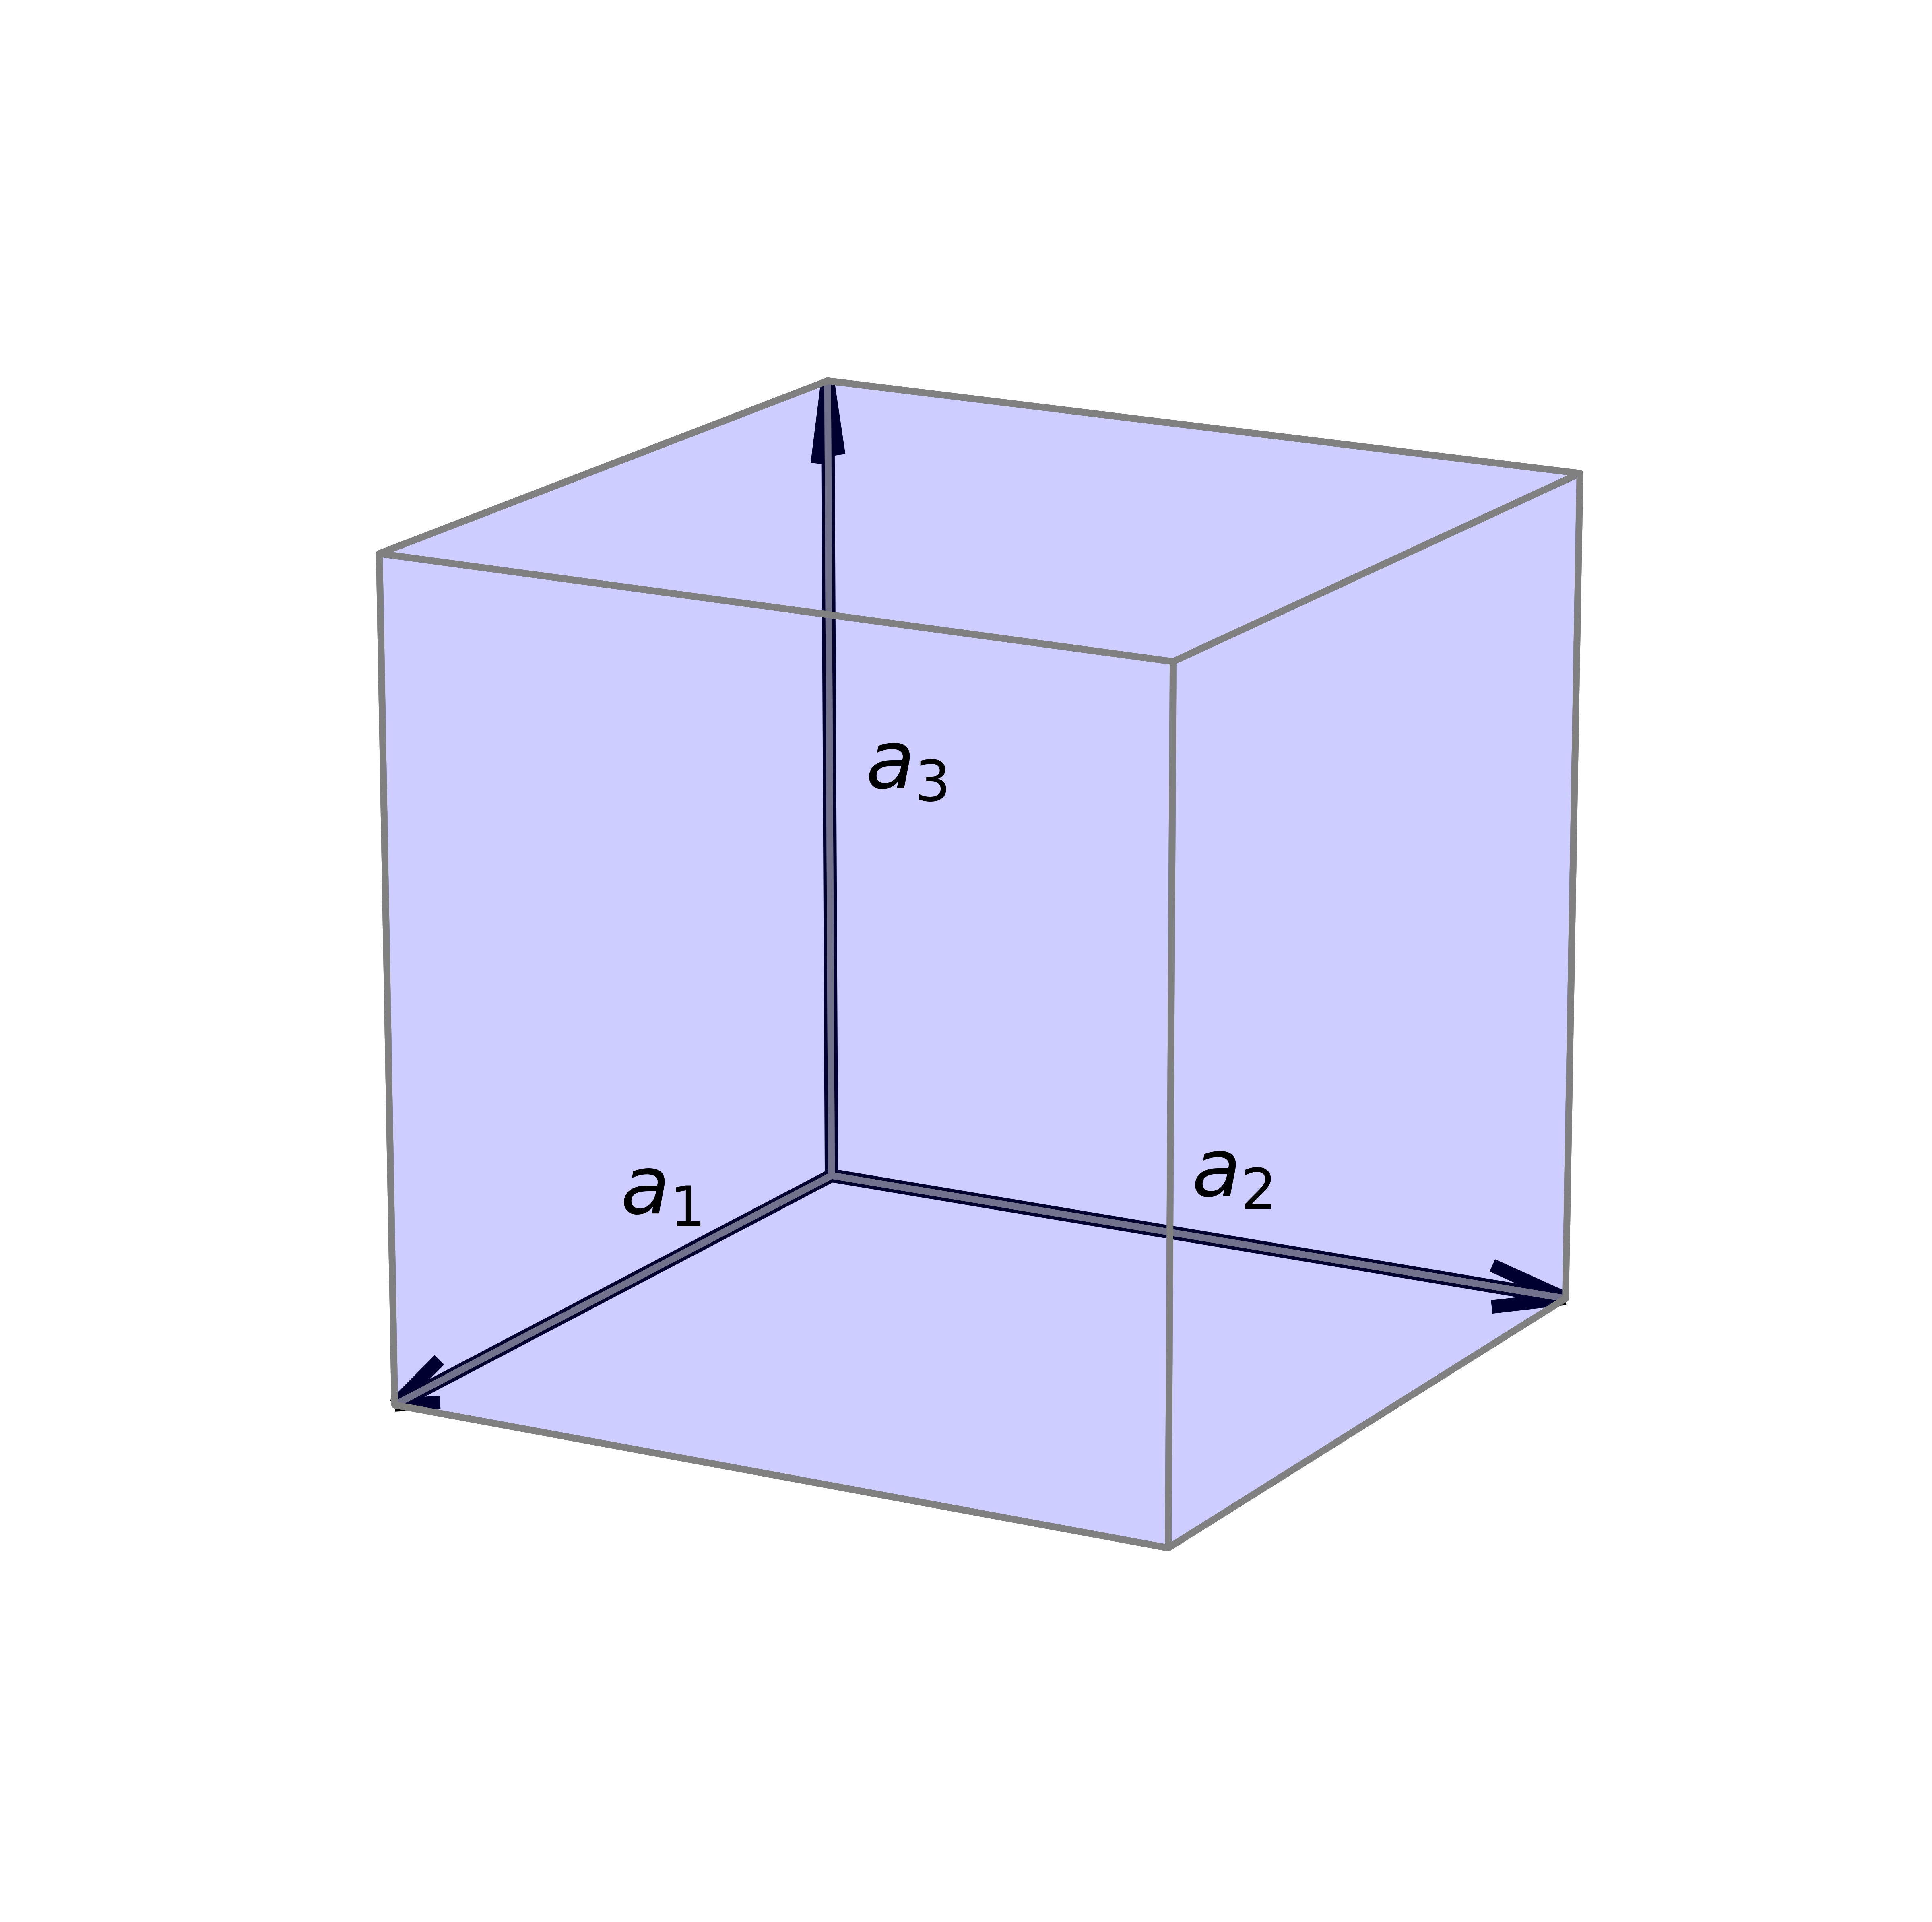
\includegraphics{chapter3/unit_cell}
  \caption{Depiction of the lattice vectors which bound the the unit cell depicted in blew.}
  \label{fig:unit_cell}
\end{figure}

The boundaries of the unit cell are defined are defined by three lattice vectors, defined in three dimensional Euclidean space, $\mathbb{R}^3$.
The three lattice vectors, $\bm{a}_1$, $\bm{a}_2$, and $\bm{a}_3$, with $\bm{a_i}\in\mathbb{R}^3$, define a coordinate sytem in Euclidean space in which to describe a lattice.

To describe the atoms, each atom is identified by a chemical species, $s\in S$, and its atomic position, $\bm{r}$.
If the atomic positions are represented in the Cartesian unit vectors, $[\hat{\bm{\imath}},\hat{\bm{\jmath}},\hat{\bm{k}}]$, then the atomic positions are the ordered triplet, $(r_x,r_y,r_z)$.
More commonly, atomic positions, $(r_1,r_2,r_3)$, are represented in the coordinates system defined by the lattice vectors $[\bm{a}_1,\bm{a}_2,\bm{a}_3]$.  The transformation from the space described by the lattice space to Cartesian space, is described by equation.
\begin{equation}
	\label{eq:fractional_vs_cartesian_coordinates}
	r_x \hat{\bm{\imath}} + r_y \hat{\bm{\jmath}} + r_z \hat{\bm{k}}
	=
	r_1 \bm{a}_1 + r_2 \bm{a}_2 + r_3 \bm{a}_3
\end{equation}

The boundaries of the unit cell describes the periodic boundary conditions, since they also reflect that translational symmetry of the crystalline system.
Each lattice vector can be represented as a translational operator, $T_i$ for ${i\in\{1,2,3\}}$, such that, $T_i(\bm{r})=\bm{r} + n_i \bm{a}_i = \bm{r}$, and collectively,
\begin{equation}
    T(\bm{r}) = \bm{r}
		    + n_1 \bm{a}_1
		    + n_2 \bm{a}_2
		    + n_3 \bm{a}_3 = \bm{r}, \forall n_i \in \mathbb{Z}
\end{equation}

Thus, the geometry for a system with $N$ atoms can be described as
	$\bm{R} = \{\bm{a}_1,\bm{a}_2,\bm{a}_3,\bm{r}_1,...,\bm{r}_N\}$,
	where the $\bm{r}_i$ is defined in an coordinate system defined by the lattice vectors..

\subsection{Empirical Interatomic Potentials}

While the actual PES for any given material system is certainly not analytical, simulations based on solving the Kohn-Sham(KS) equations of density functional theory (DFT) can provide energy calculations of sufficient accuracy for many systems.  However, the computational bottleneck associated in solving for the charge density, energy levels, and wavefunctions of the KS equation limits its adoption as a viable energy calculator to systems consisting of no more than a few hundred atoms.

In contrast, the use of empirical interatomic potentials (EIP) in molecular dynamics simulations can routinely comprise of millions of timesteps on millions of atoms.  In \emph{ab initio} simulations, the solution to the electronic structure of the system is used to calculate the energies of atomic configurations and the forces on the atoms required to evolve the system. In contrast, EIPs have an analytical formalisms consisting of formulae which represent the relevant physics of the system.  This simplification in calculation allows energies and forces drastically improved computational efficiency at the expense of simulation fidelity.

The goal of developing an interatomic potential, $\hat{V}$, is to identify a computationally efficient surrogate model, which models the potential energy surface, $V$.  The use of a hat over a variable indicates that the quantity is an approximation of the actual value.
Since energy is a scalar value, $V$ and $\hat{V}$ are functions in the same space that assigns energies to atomic configuration (e.g. ${V:\{\bm{R}\}\rightarrow \mathbb{R}}$ and ${\hat{V}:\{\bm{R}\} \rightarrow \mathbb{R}})$, we can then define the approximating relationship by the addition of a difference term $\epsilon$
\begin{equation}\label{eq:pes_approximation}
    V(\bm{R}) = \hat{V}(\bm{R}) + \epsilon(\bm{R}).
\end{equation}
In the above equation, $V(\bm{R}$ is the particular energy for a given atomic configuration $\bm{R}$, $\hat{V}(\bm{R}$ is the approximation of the interatomic potential for the same ${\bm{R}}$, and $\epsilon(\bm{R})$ is difference in energies between the two to provide energy balance to the equation.

Interatomic potentials are often expressed as a series expansion of functional terms which explain the relevant physics of a system.  In these cases, the total energy of the system is sum of the individual contribution of each atom $i$.  For a system with $N$ atoms,
\begin{equation}
	\label{eq:potential_energy}
	\hat{V}(\bm{R})= \sum_{i=1}^{N} \hat{V}(\bm{r}_i)
\end{equation}
represents the total energy of a system with $\hat{V}(\bm{r}_i \vert \bm{R})$ being the contribution of the $i$th atom of  a system.
The total energy of a potential of $N$ atoms with an interaction described by the empirical potential, $V$, can be expanded in a many body expansion as described in LeSar\cite{lesar2013_textbook}
\begin{align}
\label{eq:potential_expansion}
	\hat{V}(\bm{R}) &\equiv \hat{V}(\bm{r}_1,...,\bm{r}_N) \\
	          &= \sum_i V_{1,i} (\bm{r}_i)
	             + \sum_i \sum_{i<j} V_{2,(i,j)}(\bm{r}_i,\bm{r}_j)
		     + \sum_i \sum_{i<j} \sum_{j<k} V_{3,(i,j,k)}(\bm{r}_i,\bm{r}_j,\bm{r}_k)
		     + ...
\end{align}
Based upon this expansion, we can classify certain potentials into three classes: pair-potentials, three-body potentials, and many-body potentials.

The first term $V_1$ is the one body term, due to an external field or boundary conditions, which is typically not needed in classical potentials.  The second term $V_2$ is the pair potential; the interactions of this term is dependent the upon the distance between two atoms $\bm{r}_i$ and $\bm{r}_j$, and it is common to represent the distance between the two atoms as $r_{ij}=\lVert \bm{r}_i - \bm{r}_j \rVert^2$.  The three-body term potential $V_3$ arises when the interaction interaction of a pair of atoms is modified by the presence of a third.  In these cases, the pair-potential is typically augmented with three-body terms to express angular dependence, with $\theta_{ijk}$ typically represnting the angle formed by atoms $j$ and $k$ around the central atom $i$\cite{stillinger1985_sw}.    Few potentials employ four body terms due to the dramatic expansion in terms required to describe the interaction.  Instead, a many-body interations is used to reflect the local environment around the atom $i$.

The embedded atom method is a popular approach for modelling metals in molecular dynamics simulations.  In metallic systems, an atom is embedded in a sea of delocalized electron contributed by its neighbors.  To capture this physics, Daw and Baskes postulated an potential which consisted of the pair-wise interactions of the nuclei and an embedding energy term as a function of the host electron density created by all the other atoms in the system.  The EAM model clearly can not be written in the expansion implied by \ref{eq:potential_expansion} without including very high-order terms, but can be represented by a pair-function, an embedding energy function dependent upon the density defined by contribution of a pair-wise density function.

\begin{figure}[h]
  \centering
    \includegraphics[width=5in]{chapter3/lj}
    \caption[The Lennard Jones Potential]{The Lennard Jones potential with $\sigma=1.0$ and $\epsilon=1$, which correspond to the location and depth of the energy well respectively.}
		\label{fig:lj_potential}
\end{figure}

A set of equations, collectively referred to as a formalism, compromises an analytical potential, which decomposes the energy of an atomic configuration into the individual contributions of the terms.
One analytical formalism can be used to describe different chemical compositions with similar underlying physics.  A process of parameterization specializes these functional forms to the specific composition of chemical species, through a process known as parameterization.
If $\hat{V}(\bm{R}:\bm{\theta})$ represents an empirical interatomic potential and is parameterized by a vector of parameters, $\bm{\theta}=(\theta_1,...,\theta_n)$, then $\hat{V}(\bm{R}:\bm{\theta})$ approximates $V(\bm{R})$.

The selection of parameters for the Lennard-Jones (LJ)\cite{lennardjones1924_lj_pot} potential demonstrates simple process for the selection of parameters. The LJ potential approximates the interaction between a pair of neutral atoms, such as a noble gas.  The LJ potential is
\begin{equation}
	V_{\text{LJ}}(r_{ij}) = 4 \epsilon
    \left[
	\left(\frac{\sigma}{r_{ij}}\right)^{12}
	- \left(\frac{\sigma}{r_{ij}}\right)^{6}
    \right].
\end{equation}
The $r^{-12}$ term is repulsive due to the Pauli exclusion principle, which describes overlapping electron orbitals.  The $r^{-6}$ is the attractive long range term, describing the attraction at longer ranges from van der Waals forces.  This equation has two parameters, $\sigma$ and $\epsilon$, which can used to reproduce experimental experimental data or \emph{ab initio} calculations.  As depicted in Figure \ref{fig:lj_potential}, $\sigma$ controls the location of potential well, which is correlated to latttice parameter predictions while $\epsilon$ controls the magnitude of the interatomic interactions, controlling properties like cohesive energy.


\section{Traditional Approaches to Potential Deveopment}

In the typical use of a potential, the parameters are considered to be fixed, $\hat{V}(\bm{R}|\bm{\theta})$, and the function is considered to vary only with respect to the configuration of atoms, $\bm{R}$.  In determing the potential parameterization, the empirical potential is treated as varying due to changing the parameterization, $\bm{\theta}$, while keeping the set of atomic configurations fixed $\bm{R}$.

The process of determining the optimal parameterization, $\bm{\theta}^*$, for $\hat{V}(\bm{R}|\bm{\theta})$ is a process called fitting, which is a process of constructing a curve that has the best fit to a series of data points.  Given an EIP functional form,  the ordinary least squares approach is to minimize the square differences between $\hat{V}(\bm{R}|\theta)$ and $V(\bm{R})$ over configurational space,
\begin{equation}
\label{eq:energy_matching}
	\bm{\theta}^*
		= \argmin_{\bm{\theta}\in\bm{\Theta}}
					\sum_i \left(\hat{V}(\bm{R}_i|\theta) - V(\bm{R})\right)^2
\end{equation}
where $\bm{\Theta}$ being the set of all possible parameterizations and $i$ over all possible atomic configurations.  Since the set of possible atomic configuration $\{\bm{R}_i\}$ is infinite, the interatomic potential has to be developed from a finite set of reference configurations, $\{\bm{R}_i:i<N_{C,F}\}$, which known as the fitting set.  To ensure that $\bm{\theta}^*$ is transferrable to configurations not part of the fitting set, referred to as the testing set, $\{\bm{R}_i:i<N_{C,T}\}$.  For notational convenience, $N_C$ will refer to the number of structures in the fitting set.

\section{Force Matching Method}
Using \emph{ab initio} simulations as the representation of the PES ($V(\bm{R})=\hat{V}_{\text{DFT}}(\bm{R})$), a sequence of atomic configurations can be generated.  Typically, a DFT code is used to calculate energies for the atomic configuration and the interatomic forces for each atom in that atomic configuration. Since both energy and force data are generated in these simulations, the energy matching method described by equation \ref{eq:energy_matching} can be augmented with a force matching method of Ercolessi and Adams.\cite{ercolessi1994_fitting_forcematching}, where they define the objective function,
\begin{equation}
\label{eq:force_matching}
	C_{F}(\bm{\theta}) = \left(3\sum_{k=1}^{N_C} N_k \right)^{-1}
		\sum_{k=1}^{N_K}\sum_{i=1}^{N_k}
			\Vert \hat{\bm{F}}_{ki}(\bm{\theta}) - \bm{F}_{ki}\Vert^2.
\end{equation}
where $N_k$ is the number of atoms in configuration $k$, $\hat{\bm{F}}_{ki}(\bm{\theta})$ is the force on the $i$th atom in set $k$ obtained from the parameterization $\bm{\theta}$, and $\bm{F}_{ki}$ is the reference force from first principles calculation.

In this approach, the fitted potential becomes a surrogate for the potential energy surface estimated by the \emph{ab initio} approach, biasing the parameterization to replicate any errors that may manifest itself due to the first principles method, such as the choice of the exchange correlation functional.  For example, it is well-known that the local density approximation [27] (LDA) calculations tend to result in overbinding causing an underestimate of the lattice constants and an overestimate in the cohesive energies, phonon frequencies and elastic moduli [28].  The generalized gradient approximations (GGA) corrects this error.  The most ubiquitous GGA functional, by Perdew-Burke-Ernzerhof (PBE)[29] is known to overcorrect, as analyzed by Wu and Cohen[30].  Moreover, there is not yet a reliable way to estimate their errors beyond the empirical observation that LDA and GGA results generally span experimental values for many structural and mechanical properties.

The force matching and energy matching approach is popular for the development of modern machine learning potentials which have no functional form, but a complicated mathematical formalism with hundreds of parameters\cite{behler2016_ml_pot} which requires a large number of datapoints to prevent overfitting\cite{wood2018_snap}.

\subsection{Fitting Database}

For analytical potential development, particularly with less complicated functional forms, the computational investment required to acquire such large \emph{ab initio} datasets is unncessary.  Instead, the typical appraoch to potential development is to match the prediction of materials properties to reference values.  In this approach,  potential development comes from optimizing a potential based upon the performance to a fixed set of material properties, known as the fitting database.

In this approach, materials properties are directly related to quantities of interests (QOIs) chosen the potential developer.  The term QOI comes from the field of verification, validation, and uncertainty quantification, where the parametric uncertainty of a model propagates to create uncertainty in the predictions of the QOIs.  Adopting this notation, material properties are denoted  $\bm{q} = ( q_{1},...,q_{N_Q} )$, for $N_Q$ quantities of interest (QOI); the values predicted by a potential are denoted, $\hat{\bm{q}}= (\hat{q}_{1},...,\hat{q}_{N_Q})$.

A fitting database is a collection of structure property functions $q_i$ associated with specific atomic configurations.	The calculation of the $i$th QOI from atomistic simulation tools can be decomposed as a function of energy evaluation of the PES over the $N_{C,i}$ atomic configurations required to do the calculation,
	\begin{equation}
		q_i = q_i(\bm{R}_1,...,\bm{R}_{N_{C,i}}).
	\end{equation}
Likewise, the prediction of the QOI from a formalism, can likewise be denoted as
	\begin{equation}
		\hat{q}_i(\bm{\theta}) = \hat{q}_i(\bm{theta}|\bm{R}_1,...,\bm{R}_{N_{C,i}}).
	\end{equation}
The choice of the more compact notation indicates that once the fitting database is fixed, $q_i$ becomes a static value and $\hat{q_i}(\bm{\theta})$ becomes a function only dependent upon the vector of parameters.

Unlike force matching techniques which require a consistent set of electronic structure data to prevent numerically inconsistent data\cite{behler2016_ml_pot}, a reference value $\hat{\bm{q}}$ can be taken from experiment, calculated from \emph{ab initio} techniques, or integrated from calculations at different levels of theory.  In early efforts of potential development, potentials were developed by fitting to a few experimental numbers.	Due to the increased confidence in DFT calculations, the current trend is to include a significant amount of \emph{ab initio} data.  \emph{Ab initio} data drastically improves the reliability of potentials by allowing the sampling of regions of configuration space, which includes atomic configurations which are difficult or inaccessible experimentally.

Since DFT solve the ground state electronic structure, incorporation of these reference values into the fitting database allows fitting to structural properties which are experimentally difficult to access, such as information from kinetically unstable structures.  The incorporation of first-principles data in the fitting database significantly improves the reliability of semi-empirical potentials by sampling a larger area of configuration space, which discussed in detail in the review article by Payne \emph{et al} \cite{payne1996_dft_database}.

From a computational standpoint, at $0$ K the calculation of material properties become precise because atomic motion stops, and only a single evaluation of a parameterization needs to be evaluated against the reference value.  When the $T>0 K$, time integration through molecular dynamics is necessary to calculate these QOIs.  Shorter trajectories yield incomplete information and confound comparison of parameters with experimental values.  When many $\hat{\bm{q}}(\theta)$ has to be evaluated many times, fitting to structure property relationships which are dependent upon themodynamic ensembles for $T>0$ quickly becomes computational infeasible.

The goal of a fitting database to find to find a representative set of structures in which to calculate the structure property relationships $q_i$.  Since $\hat{q}$ is ultimately detemined from simulations on a series of atomic configurations, we can represent the energy difference between the predicted QOIs and the target QOIs.
\begin{equation}
	\epsilon(bm{\theta})=hat{q}(\bm{\theta})-q
\end{equation}
By choising a set of QOIs, the number of structures in the fitting database is effectively fixed, which reduces the computational investment required to creating the the fitting dataset, when QOIs are determined by DFT.  In addition, the time required to evaluate a parameter set is likewise reduces, an important consideration when $\hat{\bm{q}}(\bm{\theta})$ is evaluated tens of thousands of times. and the time required to determine evaluate a a parameter set again.  The collection of structure property relationships, is denoted $\bm{q}=(q_1,q_2,...q_{N_Q})$ for $N_Q$ structure property relationships.

The determination of the optimal database is a current area of interest.  Zhang and Trinkle\cite{zhang2015_bayes_fitttingdb}.  When the fitting database is defined, potential development then proceeds by the determination of the optimal database.  With the description of the fitting database achieved, our discussion turns on how this potential database can be used to obtain an optimizal parameterization, $\bm{\theta}^*$.

\subsection{Cost Function}
\label{subsec:cost_function}

Typically, the squared difference between the predicted material property values and reference values, $\epsilon_i^2=(\hat{q}_i(\bm{\theta})-q_i)^2$, are used to measure the error since these quantities are analogous to the statistical measure of variance around a mean. The goal of fitting can be described as the selection of a parameter set which minimizes all error terms,
\begin{equation}
\label{eq:moo_LS}
	\min_{\theta\in\Theta}
		  \quad  (\hat{q}_i(\bm{\theta})-q_i)^2,
						\quad i = 1,...,N_Q
\end{equation}

Since analytical formalisms preserve only the salient physics of a particular system, it is inevitable that the potentials will have limitations in their predictive performance caused by the inadequacies of $\hat{V}$ to faithfully replicate $V$.  It is not usually possible to minimize all error terms simultaneously as there are almost inevitably tradeoffs where reducing the error for one quantity of interest increases the error in another quantity of interest.  This problem is a classic problem in multiple criteria decision-making where more than one objective function needs to be optimized simultaneously\cite{miettinen1998_mcdm}.  In fitting interatomic potentials, optimal decisions need to be taken in the presence of trade-offs between conflicting objectives.

One approach to solving this problem is the use of a response data transformation to recast a multi-objective problem as a single-objective problem.  The typical approach is to couple these objective functions with a weighted sum of squares known as the cost function. Thus, instead of multiple objective functions we have a single objective function to minimize
\begin{equation}
	\label{eq:cost_function_LS}
	C(\bm{\theta})=\sum_{i=1}^{N_Q}w_i(\hat{q}_i(\bm{\theta})-q_i)^2
		\sum_{i_1}^{N_Q} \epsilon_i^2(\bm{\theta})
\end{equation}
In this equation, the weights, $w_i$, represent the preferences of the potential designer and effectively serve as the “knobs” which allow control of the parameterization. For example, for the proposed applications of the potential, obtaining precise agreement with the elastic properties may be more important than optimizing the point defect energetics or, of course, vice versa. Although the values of $w_i$ are not explicitly defined in the interatomic potential, $\hat{V}(\bm{R}|\bm{\theta})$, they clearly play a strong role in determining the optimized parameter set.  Since the values of $w_i$ are determined by the potential designer, they are in a sense arbitrary as they reflect subjective preferences upon which the model prioritizes fidelity of one material property at the expense of another.

When $\bm{w}$ is static,  UQ techniques were pioneered by Frederiksen \emph{et al.}\cite{frederiksen2004_md_bayes}, where uncertainty in the paraemters were estimated from $T > 0K$ simulations using \emph{ab initio} molecular dynamics as reference target values with aleatory certainty.  However, as $T \rightarrow 0 K$, uncertainty of the parameters decreases and vanishes to the model fit to the $0K$ reference values.  This should not be surprising as UQ techniques requiree expressing the uncertainty assoicated with each $q_i$ was a probability distribution function.  For $0$ K reference values, the aleatory uncertainty disappears and what is typically left is epistemic uncertainty which cannot be meaningly be quantified as a probability distribution, and expressing the fitting database as point estimates.

Instead, potential developers produce different parameterizations based upon fitting databases based upon similar reference databases.  The real uncertainty in potential development is driven by the choice of $\bm{w}$.  The choice of $\bm{w}$ is nontrivial, considering that this decision must be made \emph{a priori} and the potential developer may not know the implications of adverse changes in prioritizing performance of a potential for a particular material property.

Martinez \emph{et al.}\cite{martinez2013_fitting,martinez2016_posmat} describes an approximation procedure which normalizes the $w_i$ by $q_i$ and multiplies by magnitude of acceptable fractional error.  Starting with an initial estimate of the optimal parameterization $\bm{\theta}_0$ and an initial vector of weight $\bm{w}_0$. an initial parameterization is achieved through a combination of gradient descent and global optimization, resulting on an "optimal" paramaterization, dependent upon the choice of initial conditions, weight preferences, and choice of minimization methods.  Often this result is not acceptable so an \emph{ad hoc} adjustment is applied to the weights, and the process continued iteratively until an acceptable potential is acquired.  Typically, these details are not provided in literature, hindering reproducibility of the potential development process.

When the weighting scheme is used as an \emph{a priori} method, the DM is expected to represent his/her preferences in the form of weights.  Roy and Mousseau (1996) suggests that the role of weights in expressing preferences maybe misleading.  Although the relative importance of weights show the relative importance of the objective functions it is not clear what underlies this notion.  The relative importance of objective functions is usually understood globally, for the entire decision problem, while many practical applications show that the importannce typically varies for different objective function values, that is, the concept is only meaningful locally. (Podinovsky 1994).

Additionally, the minimization of the cost function is no guarantee of transferability.  A potential which is transferable can describe material properties and structures which are different from those it was fitted to.  In some general sense, the issue of transferability deals with the problem of overfitting as well as capturing the relevant physics with the correct functional form.  To assess transferability, a potential needs to adequately describe atomic configurations which are substantially different from those contained in the training set as well as material properties not in the training set.  Moreover, the parameterization of an empirical potential should be relatively insensitive to small changes in weights in the cost function.

\section{Optimization and Pareto Efficiency}

With the typical approach to potential development described, the attention of the rest of this chapter now turns to the development of a more general framework for describing the problem, and the representation of the problem as a Pareto set.  In \ref{subsec:cost_function}, multi-objective optimization was introduced by coupling the many objective function in equation \ref{eq:moo_LS} into a single cost function in \ref{eq:cost_function_LS}.  Adapting the notation of Marley and Arora\cite{marler2004_moo_survey}, the general statement of for the potential parameterization is
\begin{subequations}
	\label{eq:moo}
\begin{align}
  &\min_{\bm{\theta}}	\quad
	  &L_1(q_1(\bm{\theta}),q_1) \\
	&	&L_2(q_2(\bm{\theta}),q_2) \notag \\
	& &... \notag \\
	&	&L_{N_Q}(q_{N_Q}(\bm{\theta}),q_{N_Q}) \notag \\
  &\text{subject to} \quad
	  &g_j(\bm{\theta}) \leq 0, \quad j=1,2,...,N_g \\
	& &h_k(\bm{\theta}) = 0, \quad k=,1,2,...,N_h \\
	& &\bm{\theta} \in \bm{\Theta}
\end{align}
\end{subequations}
where $N_g$ is the number of inequality functions, $N_h$ is the number of equality constraints, and $\bm{\theta} \in \bm{\Theta}$ ensures $\bm{\theta}$ is in the feasible parameter space defined by $\bm{\Theta}$.  Here $\bm{L}_i$ are the loss functions, which are a measures of the information loss of a potential due to the $\epsilon_i$

In MOO literature, the vector $\bm{\theta} \in \bm{\Theta} \subseteq \mathbb{R}^{N_P}$ is a vector of the design variables $\bm{\theta}_i$, for $i=1,...N_P$, and $\bm{\Theta}$ is feasible design space.  $\bm{L}(\bm{\theta}) \in \mathbb{R}^{N_Q}$ are called objectives, cost functions, or criteria.

To find the best parameterization, $\bm{\theta}^* \in \bm{\Theta}$ according to a set of objective functions, which we take here to be a set of loss functions,$\bm{L}=\{L_1,...L_m\}$.  When $m=1$ the problem is a single objective optimization problem and the goal is to minimize a single loss function $f$, i.e.,
\begin{equation}
	\bm{\theta}^* = \argmin_{\bm{\theta}\in\bm{\Theta}} L(\bm{\theta}).
\end{equation}
When $m>1$, the problem becomes a multiple-objective optimization problem(MOO).  In this case, no global optimum exists since the objective functions are competing.

To remove the dependence on \emph{a priori} performance preferences, it is necessary to define an ensemble of parameterization which are optimal in a sense.
Suppose we have two parameterizations,
where $\bm{\theta}_1$ dominates $\bm{\theta}_2$,
denoted $\bm{\theta}_1 \prec \bm{\theta}_2$,
when $\epsilon_i(\bm{\theta}_1) \leq \epsilon_i(\bm{\theta}_2) \forall i \in \{1,...,N_P\}$ and $\exists i \in \{1,...n\}, \epsilon_i(\bm{\theta}_1) < \epsilon_i(\bm{\theta}_2)$.
We say that $\bm{\theta}_n$ is Pareto efficient if $\nexists \bm{\theta}_i \in \Theta, \bm{\theta}_i \nprec \bm{\theta}_1$.

The set of all parameters which produce Pareto effcient points is denoted $\bm{\Theta}^*$, and contains all non-dominated points.  While performance requirements have not yet been encoded to determine $\bm{\theta}^*$, this point must fall in the Pareto set, $\bm{\theta}^* \in \bm{\Theta}^*$.  If $\epsilon_i$ are competing, then clearly there are parameterizations which performs well with respect to $\epsilon_i$, but poorly with respect to $\epsilon_j$.

\subsection{Loss Functions}
Loss function describe the information loss for the $i$th QOI, which is the absolute difference between predicted and target values.  In machine learning strategies, literature will often refer to the its negative, the fitness function, which indicates the system of equations is to maximized rather than minimized.  Through this work, objective functions will be expressed as minimization functions.

The absolute difference function,  $L^1(\bm{\theta})=| \epsilon_i(\bm{\theta}) | = |\hat{q}_i(\bm{\theta}_j-q)|$ for the $j$th parameterization of a potential and has the benefit in that it is in same units as $q_i$.  However, when using gradient techniques, $L_1$ is not continuously differentiable at the area of interest (i.e. where $\epsilon_i =0$), which likely will create numerical instability problems.  In equation \ref{eq:cost_function_LS}, the quadratic loss function
$L^2
		=\epsilon(\bm{\theta})^2
		=(\hat{q}_i(\bm{\theta}_j-q)^2=$
is used, and has the benefits of being a continuously differentiable concave function with respect to $\hat{q}(\bm{\theta})$.  However, the continuity and convexity $L^2$ with respect to $\theta$ is not guaranteed, and is dependent upon to the continuity and convexity of $\hat{q}(\bm{\theta})$ with respect to $\theta$.

The choice of loss functions is critical for cost functions because different different loss functions will give different results given the same weighting scheme.  For examples, a cost function based on $L_1$ will give different results than a function based upon $L_2$.

For the purposes of this work, an acceptable cost function $L$ must be postive and $L$ must preserve the order with respect to $L^1$.  For any two parameterizations, $\bm{\theta}_i$ and $\bm{\theta}_j$, if $|\epsilon(\bm{\theta}_i)| < |\epsilon(\bm{\theta}_j)|$, then $L(\bm{\theta}_i) < L(\bm{\theta}_j)$.

\subsection{Parameter Constraints}

Since analytic formalas respect the relevant physics of a system, then the parameters of the formulae may have physical meaning.  An optimal parameter should represent realistic physics, such as the coefficients of attractive and repulsive terms having the correct sign.  These can be encoded as inequality constraints to enforce $\bm{\theta} \in \bm{\Theta}$.

Moreover, it may also be desirable to impose equality constraints on the parameters.  In charged systems, it is desireable to have charge balance.  For example, for magnesium oxide (MgO), it is necessary to have the charges of the magnesium and oxygen ions to balance, $Z_{\text{Mg}} = Z_{\text{O}}$ to be equal.  These can be encoded as equality constraints.

Finallly, there may be constraints upon QOIs we may want to impose.  For example, the formation energy for the ground state atomic configration (in eV/atom) should be the minimum on the convex hull for competing phases.  Otherwise it would decompose into other compounds with lower energies.  For nickel, the face-cented cubic structure (FCC) is the expected ground state.  In addition to fitting the phase difference between FCC and the competing phase.  It is also desireable to impose the restriction that phase difference is positive.

\subsection{Pareto Efficiency}

To address the problem of weights, a further discussion of Pareto efficiency is necessary. This concept was first introduced by Vilfredo Pareto to model the allocation of resources in an economy\cite{pareto1897_pareto}.  Pareto was the first to realize that cardinal utlity could be dispensed with and be replaced with ordinal utlity\cite{aspers2001_pareto}.  It was not necessary to know how much someone valued a product $X$ or a product $Y$, but only to know that product $X$ is preferable to product $Y$.  As a result, the notion of total aggregate utility to represent the greatest good for the greatest number of people is replaced in modern economic with the notion of Pareto optimality, the idea that a system is maximized when no one can be made better off without making someone else worse off.\cite{mathur1991_pareto}.

In multiobjective optimization problems, it is characteristic that no unique solution exists, but a set of mathematically equally good solutions can be identified.  These solutions are known as nondominated, efficient, noninferior or Pareto optimal solutions.  In MOO literature, these terms are synomous.

Likewise, in the field of potential development the use of a cost function unnecessarily constrains potential development to encode a subjective preference for performance preferences by assigning a vector of weights to correspond with the vector of sum squared errors.  This is ultimately a subjective determination by the potential developer, and the potential developer is ultimately unable to express these preferences \emph{a priori} because knowledge in the relative tradeoffs is necessary to make an informed decision.  Instead of determining $bm{\theta}*$ with a cardinality loss function, which aggregates the subobjective function, one can calculate the Pareto surface to determine $\bm{\Theta}^*$.  Since these potentials are Pareto efficient, the decision then becomes choosing $\bm{\theta}^* \in \bm{\Theta}^*$.

Since all objective functions are to be minimized, a feasible solution $\bm{x}_1$ is said to dominate another feasible solution $\bm{x}_2$, denoted $\bm{F}(\bm{x}_1 \succ \bm{x}_2)$, if and only if $F_i(\bm{x}_1)\leq F_i(\bm{x}_2)$ for $i = 1,...,k$ and $F_j(\bm{x}_1)< F_j(\bm{x}_2$) for at least one objective function $j$.  A solution is said to be Pareto optimal if it is not dominated by any other solution in the solution space.

\begin{figure}[h]
	\centering
  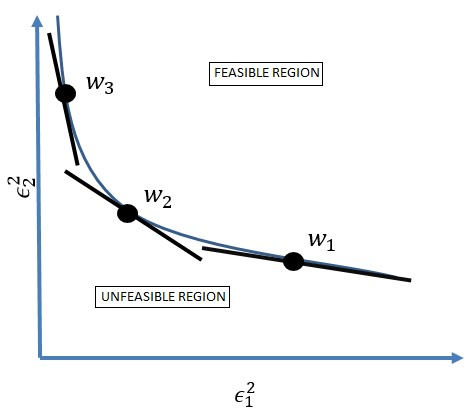
\includegraphics{chapter3/pareto_schematic}
  \caption{Schematic of a Pareto front for the differences, $\epsilon_1$ and $\epsilon_2$, between predicted and actual values for two arbitrary material properties.  The Pareto surface separates regions which are feasible and unfeasible.  Since points in the unfeasible region represent regions of unobtainable accuracy, the Pareto surface forms a boundary of the best possibilities with tradeoffs occurring on the convex hull. }
  \label{fig:pareto_convex}
\end{figure}

Figure \ref{fig:pareto_convex} provides a schematic in 2D, which allows us to illustrate this concept more concretely.  By the definition of Pareto optimality, the Pareto curve separates the feasible region from the infeasible region.  The points $w_1$, $w_2$. amd $w_3$ dominate some of the points on the interior of the Pareto curve, but they do not dominate each other.  The point $w_1$ has better performance with respect to $q_2$ at the expensive of $w_3$, while the fortunes are reserved for $w_3$.  The point $w_2$ is a compromise position between the two.  Without the expression of preferences, one is indifferent to the selection of any of these potentials, but it is rational to choose any of them since they are all Pareto efficient.  If an vector weights was chosen \emph{a priori}, then the potential developer is making a decision about the optimal parameterization without regard to tradeoffs in performance in the fitting set.

The shape of the Pareto front provides valuable insights into the performance of a potential formalism.  In this case, the Pareto front is monotonically decreasing and convex.    Suppose, we start with an initial set of weights $\bm{w}_1$, with the goal of reducing $\epsilon_1$.  A change in the weights to $\bm{w}_2$ places a larger preference on reducing $\epsilon_1$ at the expense of increasing $\epsilon_2$.  Due to the slope of the tangent line implied by the weights, a large reduction in $\epsilon_1$ is possible with only a small sacrifice in $\epsilon_2$.  However, continual improvements in reducing $\epsilon_1$ by changing the weights has a diminishing effect due to the convexity of the Pareto front.  A change in the weights from $\bm_{2}$ to $\bm{w}_3$ will still reduce $\epsilon_1$ at the expense of increasing $\epsilon_2$.  Compared to the previous change, a small reduction in $\epsilon_1$ comes with the tradeoff of a large increase in $\epsilon_2$.

\section{Multiobjective Optimization Methods}
A multi-objective optimization approach should achieve the following conflicting goals as described by Zitzler \emph{et al.} \cite{zitzler2000_moo_evolve}: (1) the best known Pareto front should be as close as possible to the true Pareto front.  Ideally, the best-known Pareto set should be a subset of the Pareto set, (2) solutions in the best known Pareto set should be uniformly distributed and diverse over the Pareto front in order to provide the decision-maker a true picture of trade-offs, and (3) the best-known Pareto front should capture the whole spectrum of the Pareto front at the extreme ends of the spectrum.  While the first two goals are important for multi-objective optimization, the last goal is erroneous.  In potential development, compromise solutions are desireable; a potential with high fidelity with respect to one material property at the expense of a loss of fidelity with respect to all other predictions is pathological.

\section{Solution Methods}
Weights that produce a certain Pareto optimal solution are not necessarily unique, and different weights may produce similar solutions.  On the other hand, a small change in weights may cause big differences in the objective function.  It is not easy for the potential developer to control the solution process because weights behave in an indirect way.  The solution process then becomes interactive, where one tries to guess the weights that would produce a satisfactory solution.  When the tools for potential development to not adequate to support the potential developer in such an \emph{ad hoc} approach, the process leads to frustration and complications in potential development.  In this case, it is advisable to develop a real interactive method where the solution process can be better controlled so that the potential developer can provide more intuitive preference information.

By calculating the Pareto set before analysis and selection, the whole problem of expressing preferences disappears and the traditional analysis approach can proceed in an interactive way.  In addition, provides a wealth of information into all the different rational parameterization, enabling applications such as parametric uncertainty as an input to feed foward to uncertainty quantification methods, shortcomings of potential formalisms, and correlations of errors between computationally inexpensive testing set QOIs to more expensive $T>0$ simulations, which are used to calculate key material properties in engineering applications and larger scale simulations.

\subsection{Pareto Optimization from Cost Function Optimization}

In potential development, the preferences of potential developer influences are particular parameterization, which has the result that the development of empirical potentials is somewhat of a black art.  Here, we demonstrate that the choice of using local optimization tools, as sparsely documented methods for overcoming the weaknesses of local optimization requires considerable skill and experience on the potential developer, as it is difficult to obtain the Pareto surface using traditional techniques.

Let us consider the unlikely case that our potential optimization problem, $C(\bm{\theta},\bm{w})$ is a convex function with respect to $\theta$ and $\nabla C$ being Lipschitz.  Then for an initial condition $\bm{\theta}_0$, we can numerically construct a sequence, ${\bm{\theta}_t}$,
\begin{equation}
	C(\bm{\theta}_{t+1}) < C(\bm{\theta}_{t}), \qquad t = 0,1...
\end{equation}
In each direction, we search in the descent direction informed by the gradient, $\nabla C(\bm{\theta}_t)$ by step size $\eta_t$ to determine $\bm{d}$, the distance to move.  In the gradient descent algorithm, the descent direction is $\bm{d}_t = - \nabla C(\bm{\theta}_t)$.  This process continues until convergence conditons are met to achieve the numerical approximation at $C(\bm{\theta}^*)$.  Any unique vector of weights $\bm{w}$ will result in the optimal parameterization with respect to the selection of weights.  Since $C(\bm{\theta}|\bm{w})$ evaluated at $\bm{\theta}^*$ is a constant, the vector of weights will also define the hyperplane tangent to the pareto surface,
\begin{equation}
	\sum_{i=1}^{N_Q} w_i L_i = C(\bm{\theta}^*)
\end{equation}

In the development of interatomic potentials, the DM is asked to specify weights in which case the method is used as an \emph{a priori} method.
To estimate the Pareto surface, it is sufficient to select a set of weightings.  Since our function is convex and Lipschitz, each unique selection of $\bm{w}$ will give a different point on the Pareto surface as the schematic in figure \ref{fig:pareto_convex}.

The weighting method can be used as an \emph{a posteriori} method where different weight can be used to generate different Pareto optimal solutions, and then themost satisfactory solution selected afterwards.  Systemic methods of perturbing the weights to obatain different Pareto optimal solutions are suggested (Chankong and Haimes 1983), but Das and Dennis 1997 illustrates that an evenly distributed set of weights does not necessarily produce an evenly distributed representation of the Pareto optimal set, even when the problem is convex.
%https://books.google.com/books?id=NHZqCQAAQBAJ&pg=PA1&source=gbs_toc_r&cad=4#v=onepage&q&f=false

The use of local optimization techniques in potential development are clear: local optimization methods are fast, can handle large scale problems, and are largely applicable to a large range of potentials, since they only require differentiability of the objective function and the constraint function\ref{boyd_convex_optimization}.  When Karush-Kuhn-Tucker conditions\cite{karush1939_kkt,kuhn1951_kkt} are met for the constrained optimization parameter optimation problem, solutions remain fairly computationally tractable because of the maturity of the technology and methods associated with gradient based methods and linear algebra techniques.

Algorithms for multiobjective optimization should produce Pareto optimal solutions, and that any Pareto optimal solution can be found.  In this respect, the weighting method has a serious shortcoming.  Any Pareto optimal solution can be found by altering weights only if the problem is convex.  Some Pareto optimal solutions of nonconvex problems cannot be found regardless of how the weights are selected.  In potential parameterization, the compromise is to give up seeking the optimal $\bm{\theta}$, which minimizes the objective over all feasible points.  To solve the problem as a constrained minimization problem with subject to the usual inequality and equality constraints, $g_i(\bm{\theta})$ and $h_j(\bm{\theta})$.  The problems of the weighting schemes have ben explored by the classical potential development community.\cite{martinez2013_fitting}  The method may jump from one vertex to anohter vertex leaving intermediate solutions undetected with relatively small changes in the weighting schemes.\cite{martinez2013_fitting}

Instead, the choice the process is to seek a point that is only locally optimal, which means that it minimizes the feasible points which are near it.  The disadvantages of local optimization methods go beyond not finding the true, globally optimum solution.  The initial guess, $\bm{\theta}_0$ is critical, and can greatly affect the objective value of the local solution.  Little information is provided on how far from the globally optimal solution the local solution is.  In addition, local optimization methods are sensitive to the choice of algorithm, algorithm parameter values, which maybe need to be adjusted based upon the $C$ to $\bm{theta}$ response surface.

One way to overcome the problem with poor initial conditions, is to optimize the cost function from multiple initial conditions.  Given the upper and lower bound of $\bm{\Theta}$ for each parameter $\bm{\theta}$, one can construct an a a grid of initial conditions from which to start the local optimization routine.  As we will demonstrate later, this technique is computationally expensive as the gradient descent paths from each initial condition to achieve optimal solution, $\bm{\theta}^*(\bm{\theta}_0,\bm{w})$, which grows with the density of the grid, the dimensionality of the $q$-space, and the dimensionality of $\theta$-space.

As a result, potential developers have begun to experiment with global optimization techniques, such as genetic algorithms and simulated annealing\cite{martinez2013_fitting,martinez2016_posmat}, to obtain a true global solution of the optimization problem.  However, the compromise in these cases is efficiency.  As the potential formalism increases, the computational complexity of global optimization techniques also increases exponentially.

\section{Pareto Optimization from Monte Carlo techniques}

Genetic algorithms are a popular meta-heuristic that is particularly well-suited for this class of problems.  Traditional GA are customized to accomodate multi-objective problems by using specialized fitness functions and introducing methods to promote solution diversity.  The method which will be proposed in chapter 5 is not a genetic algorithm, but is designed as an evolutionary algorithm which reduces the epistemic uncertainty of parameterization, but evolving the distribution into a distribution  which describes the parameters which produces Pareto optimal results.

The previous section described how the Pareto surface could be estimated for a convex cost function, by selecting an initial condition and solving for the optimal parameterization given set of weights, then repeating the process by varying the weighting scheme.  However, when the cost function is not convex, the process becomes a local solution process and more computationally expensive techniques are necessary.  This can involve assessing multiple starting parameterizations and applying global optimization techniques.  More problematically, much of the information calculated from many evaluations of the cost function other than the final solution (given an initial condition and a weighting vector) is lost.  Even if the information was retained, it is unclear how to integrate that information to more efficiently calculate a Pareto surface.

In a deterministic approach we would want to identify an algorithm such that we start with feasible set of parameterizations and constrains the sets of parameterizations until it produces a set of parameterizations which produces a set of optimal parameters $\bm{\Theta}^*$, which produces Pareto-optimal results $\epsilon$-space.  Here we propose a technique that takes advantage of Monte Carlo sampling.  While Monte Carlo solutions converge slowly, the error of estimamtion decreases as $1/\sqrt{N}$, unlike deterministic search methods that depend expend exponentially on the dimension\cite{caflisch1998_mc}.

The main idea behind this method is that results are based on repeated sampling.  Here we assume that $\bm{\Theta}$ is a random variable, with a probability distribution function which encompasses the information we know about the parameter space.  When we have much information about the parameters, we can use a uniform distribution defined by upper bound and lower bound for each parameter.  Since $\bm{\theta}$ is now a realization of the random variable $\bm{\Theta}$, for each $\bm{\theta}_i$ we can produce $\hat{\bm{q}}_i(\bm{\theta})$ by running these simulations against our simulation machinery.  Moreover, this method is trivially parallelizable.

To determine the estimate $\bm{\Theta}^*$ is determined the following algorithm.  Given the set of QOI evaluations, $\hat{\bm{Q}}=\{\hat{\bm{q}}()\bm{\theta}_1),...,\hat{\bm{q}}_i{\theta}\}$ calculate the Pareto optimal set using the definition of the Pareto optimality, $\hat{\bm{Q}}^* \subseteq \hat{\bm{Q}}$.   The parameters which produce the elements in $\hat{\bm{Q}}^*$, are the set of parameters which produce the Pareto optimal parameters.

The convergence of this algorithm can be drastically improved by updating the probability distribution based upon the results of previous simulations.  In chapter 5, we discuss this process in more detail.

\subsection{Computational and Performance Comparison}
 The performance of these algorithms were tested against the well known problems of Schaffer\cite{schaffer1984_pareto} and Kurasawe\cite{kursawe1991_pareto} to demonstrate the relative performance computational cost of these approaches.  Both of these problem only have two objective functions, which makes visualization of the concepts more concrete.

 awe can produce as many samples to evaluate for performance against the fitting database to produce $\bm{q}.$  When a large enough amount of samples are evaluated,
 It is a generic solution and the iterative approach of generating new populations is akin to previous solutions.
 increases with the increase in the number of objectives.

 The ultimate goal of a multi-objective optimization algorithm is to identify solution in the Pareto optimal set.  However, identifiying the entire Pareto optimal set, for multi-objective problems, is impossible to its size.  Proof of solution optimality is computationally infeasible.  Therefore, a practical approach is achieve successively better approximations of the Pareto surface that represent the Pareto set as well as possible.

 The first of the test optimization function of a smooth convex multi-objective optimization problem described by Schaffer\cite{schaffer1984_pareto}.  Here the multi-objective function $F:\mathbb{R} \rightarrow \mathbb{R}^2$.

 \begin{equation}
 \begin{aligned}[t]
   &\min_{x} \quad
      &\begin{aligned}[t]
            &f_1(x) = x^2 \\
            &f_2(x) = (x-2)^2 \\
       \end{aligned}
 \end{aligned}
 \end{equation}

The second test optimization problem of Kurasawe.
\begin{equation}
\begin{aligned}[t]
  &\min_{\bm{x}}
    &\begin{aligned}[t]
      f_1(\bm{x}) &= \sum_{i=1}^2
          \left[
            -10 \exp\left(-0.2 \sqrt{x_i^2} + x_{i+1^2}\right)
          \right] \\
      f_2(\bm{x}) &= \sum_{i=1}^3 \left[ \vert|x_{i} \vert|^{0.8} + 5\sin(x_i^3)\right] \\
    \end{aligned}
  \\
  &\text{subject to}
    &\begin{aligned}[t]
		      -5 &\leq x_i \leq -5 \\
      		 1 &\leq i   \leq  3 \\
    \end{aligned}
  \end{aligned}
\end{equation}

\begin{figure}[h]
	\centering
  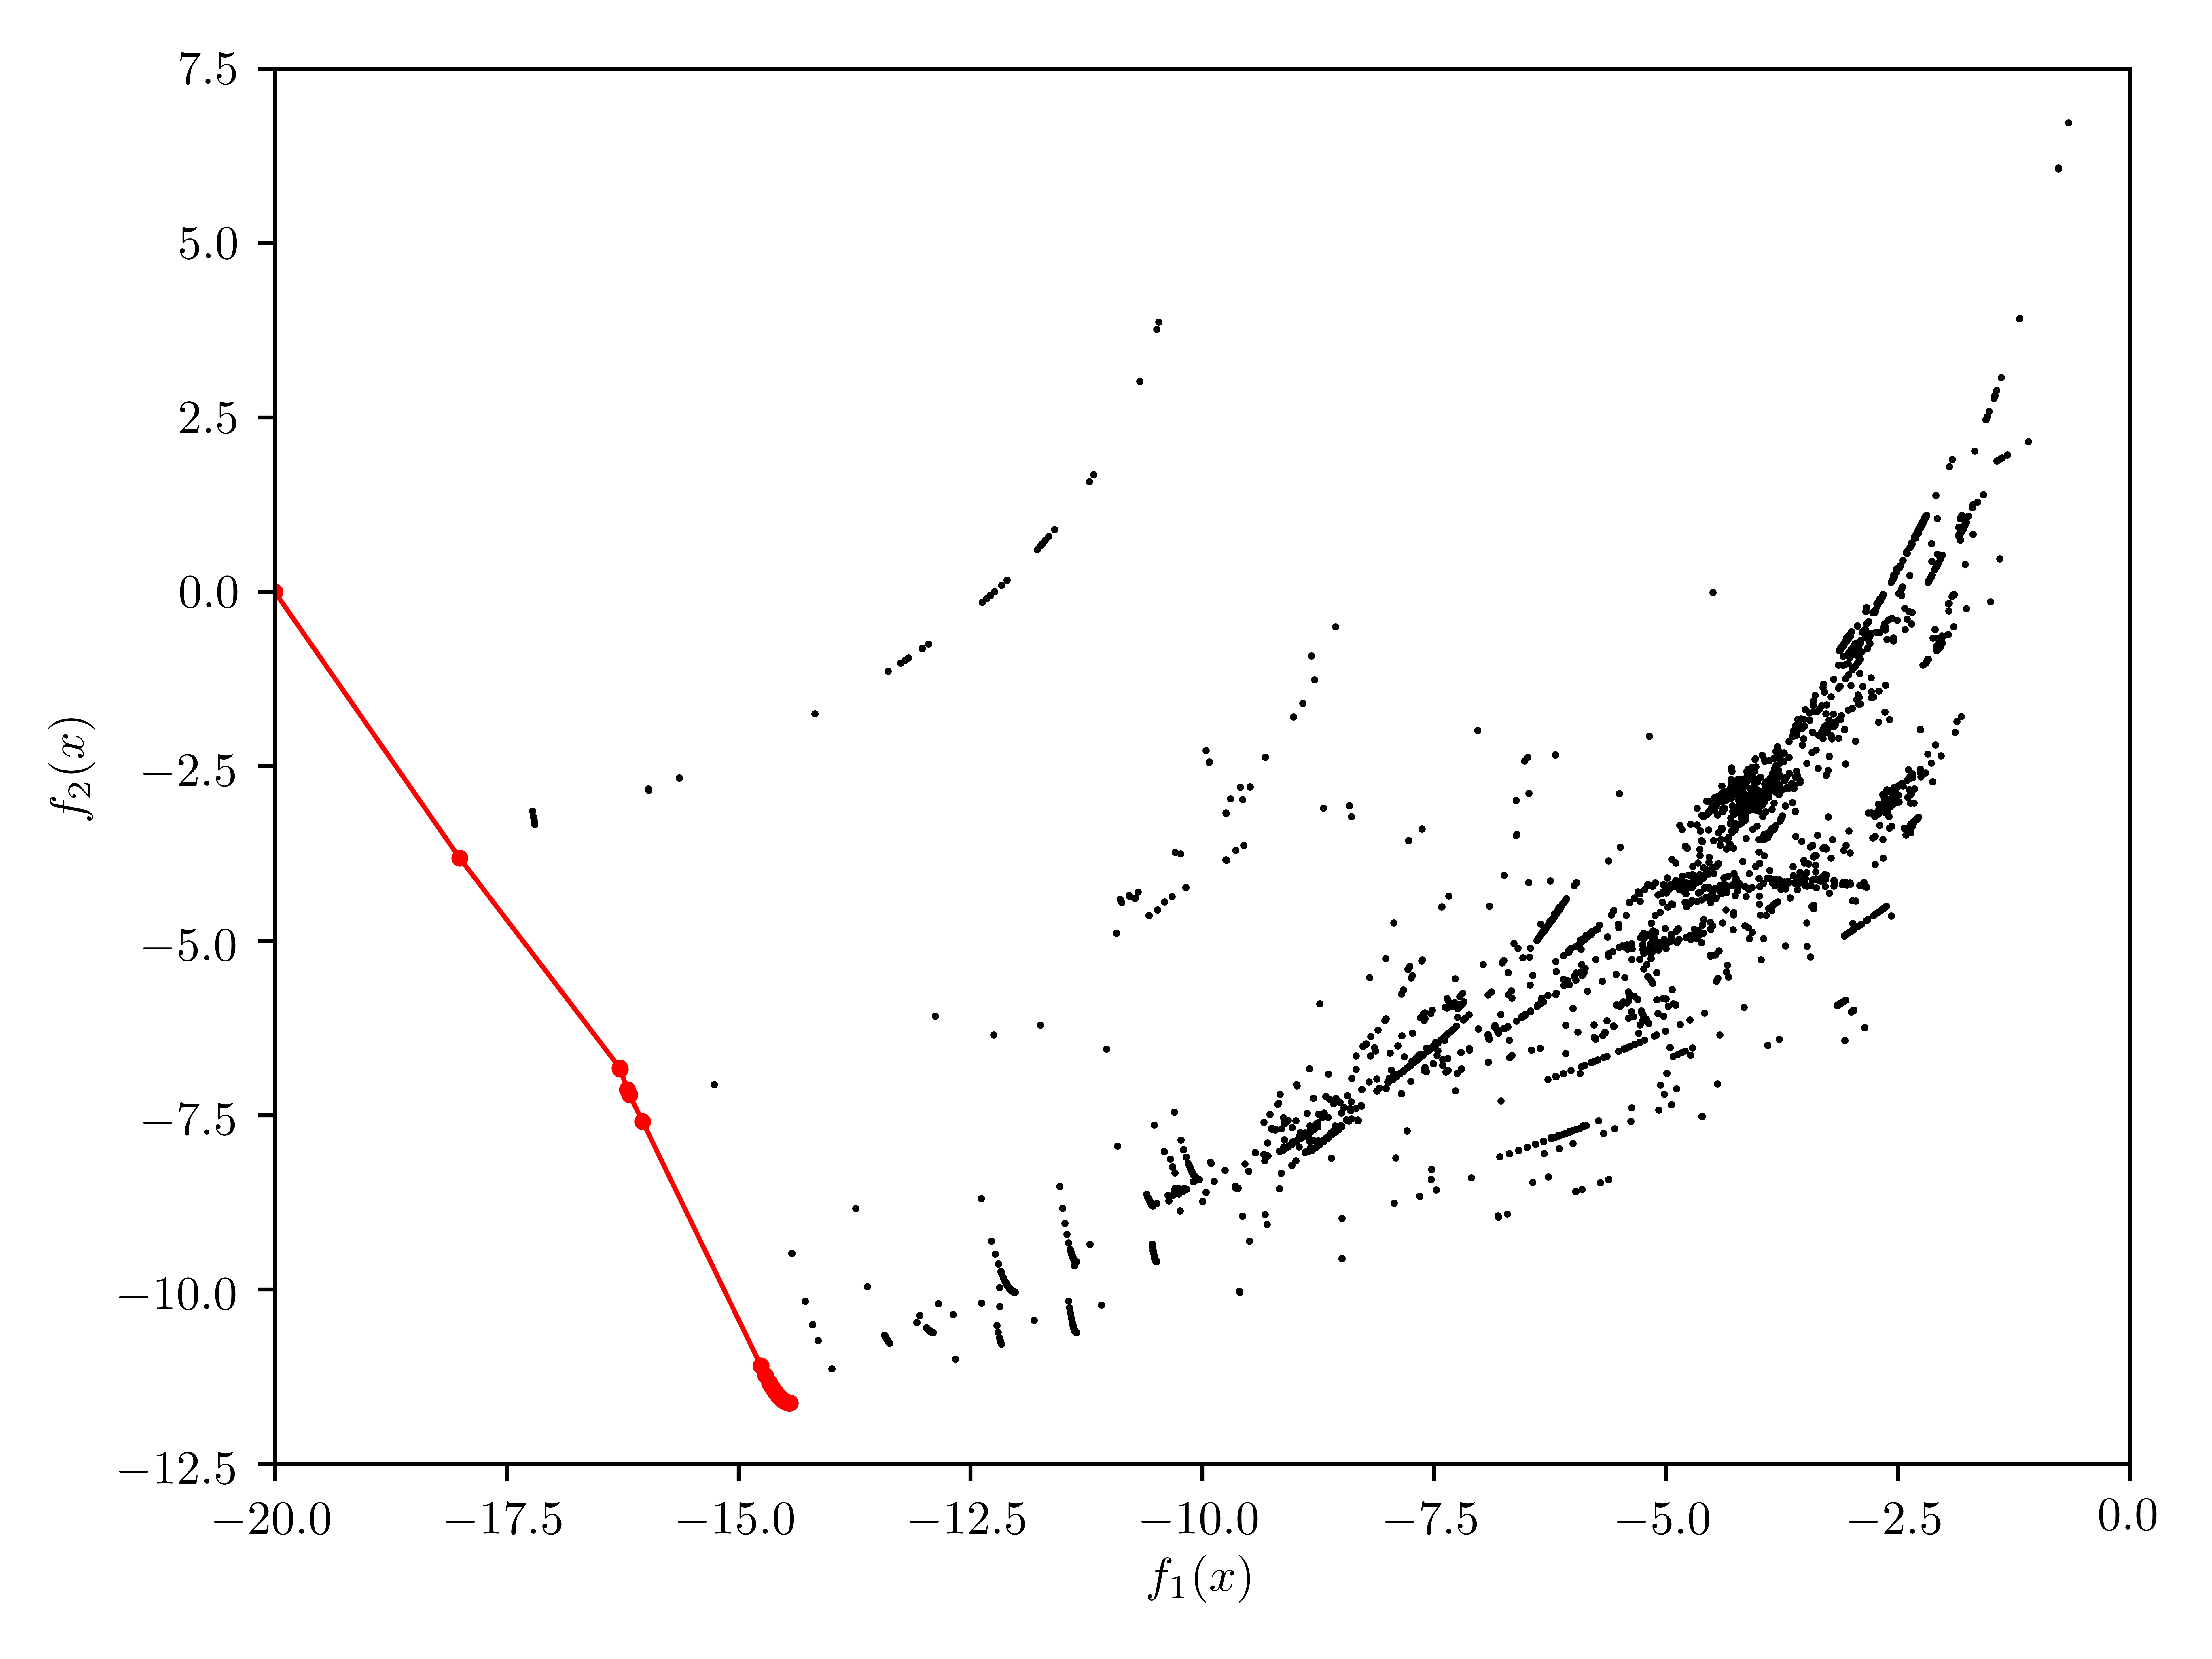
\includegraphics{chapter3/kurasawe_cg}
  \caption{Schematic of a Pareto front for the differences, $\epsilon_1$ and $\epsilon_2$, between predicted and actual values for two arbitrary material properties.  The Pareto surface separates regions which are feasible and unfeasible.  Since points in the unfeasible region represent regions of unobtainable accuracy, the Pareto surface forms a boundary of the best possibilities with tradeoffs occurring on the convex hull. }
  \label{fig:kurasawe_cg}
\end{figure}

\begin{figure}[h]
	\centering
  \includegraphics{chapter3/kurasawe_mc}
  \caption{Schematic of a Pareto front for the differences, $\epsilon_1$ and $\epsilon_2$, between predicted and actual values for two arbitrary material properties.  The Pareto surface separates regions which are feasible and unfeasible.  Since points in the unfeasible region represent regions of unobtainable accuracy, the Pareto surface forms a boundary of the best possibilities with tradeoffs occurring on the convex hull. }
  \label{fig:kurasawe_mc}
\end{figure}

\begin{figure}[h]
	\centering
  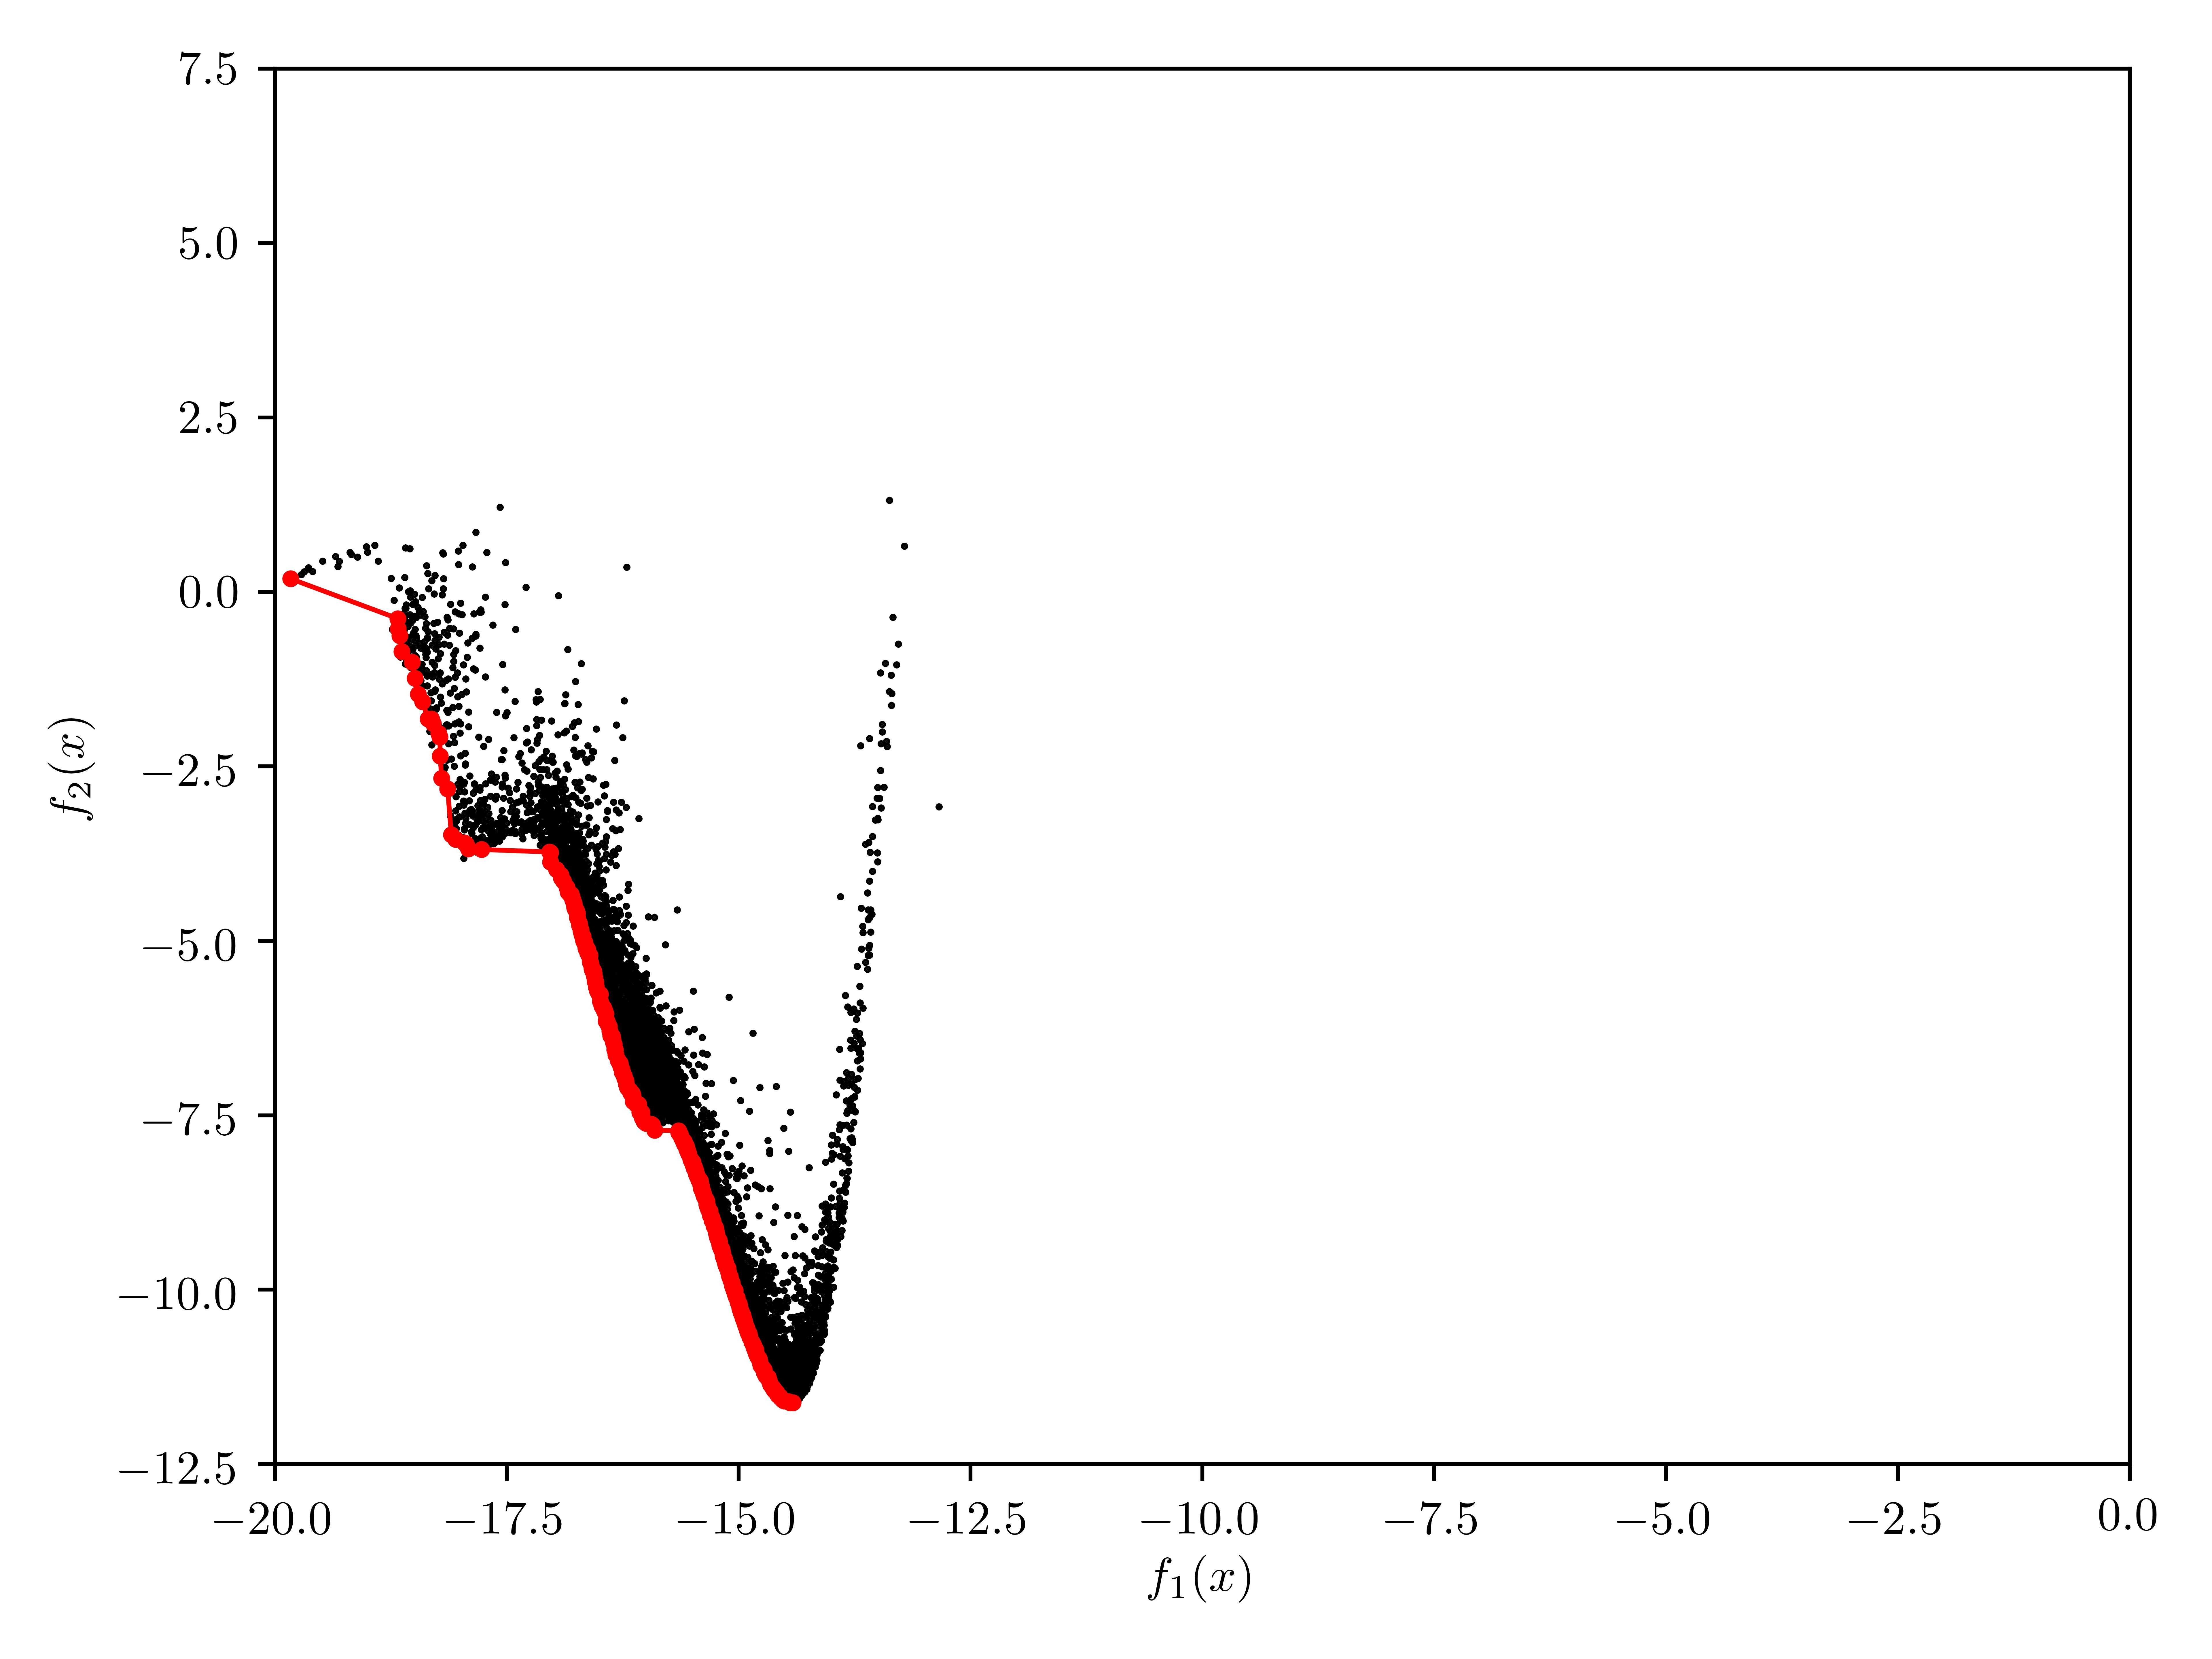
\includegraphics{chapter3/kurasawe_kde}
  \caption{Schematic of a Pareto front for the differences, $\epsilon_1$ and $\epsilon_2$, between predicted and actual values for two arbitrary material properties.  The Pareto surface separates regions which are feasible and unfeasible.  Since points in the unfeasible region represent regions of unobtainable accuracy, the Pareto surface forms a boundary of the best possibilities with tradeoffs occurring on the convex hull. }
  \label{fig:pareto_convex}
\end{figure}

\begin{figure}[h]
	\centering
  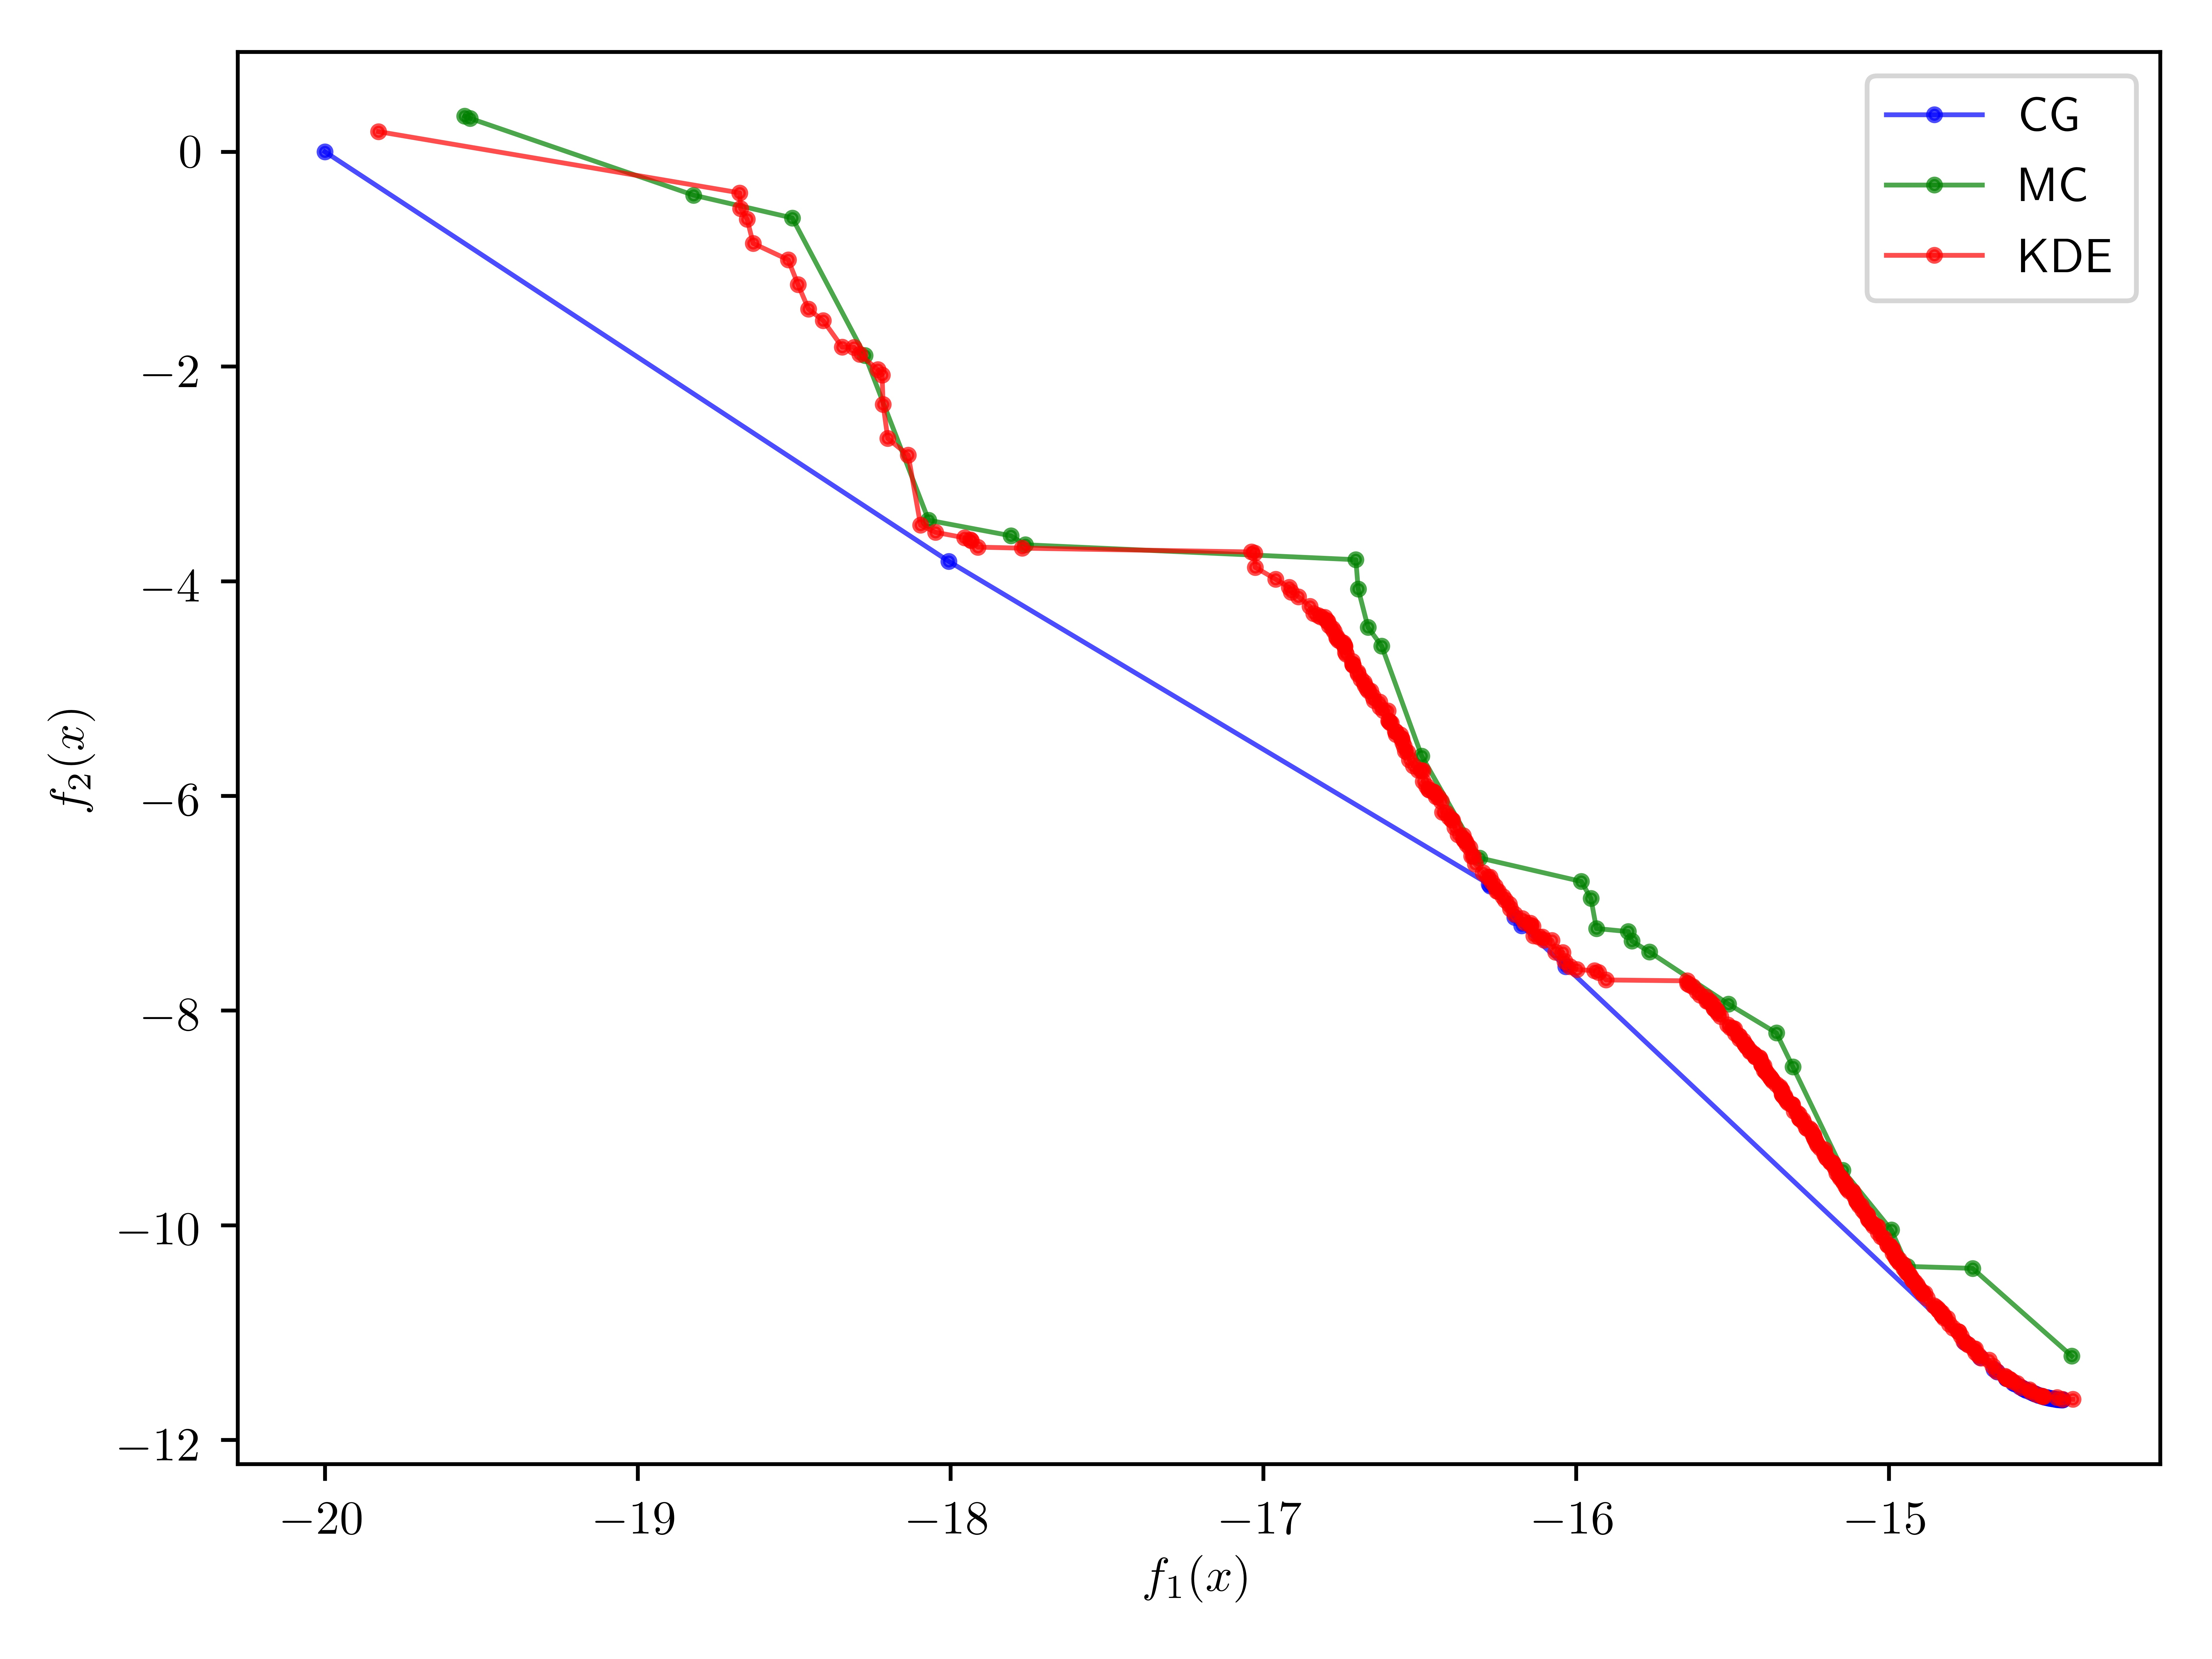
\includegraphics{chapter3/kurasawe_comparison}
  \caption{Schematic of a Pareto front for the differences, $\epsilon_1$ and $\epsilon_2$, between predicted and actual values for two arbitrary material properties.  The Pareto surface separates regions which are feasible and unfeasible.  Since points in the unfeasible region represent regions of unobtainable accuracy, the Pareto surface forms a boundary of the best possibilities with tradeoffs occurring on the convex hull. }
  \label{fig:kurasawe_comparison}
\end{figure}

\begin{table}[ht]
	\caption{Computational comparison between gradient methods and simulation methods against the Kurasawe MOO problem}
	\label{table:kurasawe}
	\centering
	 \begin{tabular}{cccc}
		 \hline
		 d & CG method & MC method & KDE method \\
		 \hline
		 Function Evaluations & 1053132 & 100000 & 10000 \\
 		 Pareto points & 22 & 311 & 508 \\
		 \hline
	 \end{tabular}
\end{table}
 % PARETO
\chapter{PROBABILITY METHODS}
\label{ch:probability}

Due to heavy use of simulation methodology involves in this work, a discussion of probability and simulation concepts to clarify terminology and notation.  What follows is a necessarily brief introduction to probability theory in a more rigorous sense, we refer the reader to classic textbooks of Rudin\cite{rudin1987_realanalysis} for a rigorous treatment of measure theory and Chung\cite{chung2001_probabilitytheory} for a measure theory construction of probability.

\section{Probability}
The discussion of the probability methods used in this work starts with the probability construction by Kolmogorov, which builds probability as a measure of sets, but adapted to the particular necessities of probability.

Let $(\Omega,\mathcal{F},\mathbb{P}$ be a measure space with $\mathbb{P}(\Omega)=1$.  Then $(\Omega,\mathcal{F},\mathbb{P}$ is a probability space, with sample space $\Omega$, event space $\mathcal{F}$, and probabilty measure $\mathbb{P}$.  The underlying foundation of any probability  distribution is the sample space, which is the set of all probable outcomes denoted as $\Omega$.  The realization of an outcome is denoted $\omega \in \Omega$.

The events for the measure space are defined in such a way that a probability measure can be assigned.  This allows to assign probability measures on complex events to characterize groups of outcomes.  The collection of all such events is a $\sigma$-algebra $\mathcal{F}$ of subsets of $\Omega$.  Not every subset of the sample space $\Omega$ must be considered an event, the $\sigma$-algebra restricts $\mathcal{F}$ to subsets of $\Omega$ for which $\mathbb{P}$ can be asssigned.

The probability measure, $\mathbb{P}$, a function which maps $\mathbb{P}:\mathcal{F}\rightarrow[0,1]$.  A probability is a real number between zero and one.  Within this work we do not disguish the difference between impossible events which have probability zero, and probability-zero events which are not necessarily impossible.  Events of probability one is an event that happens almost surely, with almost total certainty.

The triplet $(\Omega,\mathcal{F},\mathbb{P})$ is the probability measure space.

\subsection{Probability Measures for Continuous Variables}

\subsubsection{PDF}

\subsubsection{CDF}

\subsubsection{JPDF}

\section{Interpretation of Probabilities}

The meaing of probabilities assigned to potential values of a random variable is not of probability theory itself, but instead related to philosophical context over the interpretation of probability.  In most scientific application, the probability interpretation is physical in nature, in which probabilities are objective and an event's probability is the limit of its relative frequency as the number of samples becomes large.  This interpretation supports the statistical needs and inference requirements for experimental scientists since probabilities can be found by a repeatable objective process (e.g. experiments), and are thus devoid of opinion.  Within this context, probabilities are \emph{aleatory}.  Uncertainty is irreducible and inherent to to the physical process observed.

For finite temperature simulation above $0$ K, molecular dynamics simulations allow sampling from themodynamic ensembles.  Although the simulations are replicable since time-integration and the empirical potential are deterministic.  Sampling from the time-series or by randomly assigning initial velocities, allows molecular dynamics to model aleatory uncertainty associated with a model.

Within this work, probabilities are evidentiary and can be assigned to any problem statement, even when no random process is involved, as a way to represent subjective plausibility, or to the degree in which the statement is supported by available evidence.  Evidential probabilities here are considered to be degrees of belief, such as the Laplace interpretation where probabilities are defined in disposition to gamble at certain odds\cite{laplace_probability}.  Here, conherent subjective belief systems follow the laws of probability\cite{ramsey_probability,definetti_probability}.  Here, uncertainty is \emph{epistemic} and is based on current evidence, but is mutable based upon receiving new observations\cite{ramsey2016truth,definetti1980_foresight,jaynes2003_probability}.  This philsophical interpretation is more closely associatiated with Bayesian inference.

In practice, the uncertainty associated with any problem has both \emph{aleatory} and \emph{epistemic} components.  Within this context, the field of uncertainty quantification\cite{oberkamph} in involved the quantitative characterization and reduction of uncertainties in both computational and real world applications.  The difficulty of applying Bayesian frameworks to potential development is the evidence is constrained to the size of the dataset, a parameterized potential likely produced biases due to the inevitable tradeoffs in assigning preferences in predicting various material properties.  Moreover, the inability to define the uncertainities associated target properties frustrates standard VVUQ and Bayesian approaches.

 Neither of these interpretation is particularly useful for our application.  Here, the probability distribution should be interpreted as propensities.  In the propensity theory of probability, is the probability of an event to produce an outcome of a certain kind, or to yield a long-run relative frequency of such an outcome.  Propensities are not relative frequencies, but the purported causes of the observed stable relative frequencies.

Regardless the choice in the interpretation of the meaning of probabilities, the mathematics works the same.

Formally, a continuous random variable is a random variable whose cumulative distribution function (CDF) is continuous everywhere\cite{bertsekas2002_probabilitytheory}.  More practically, random variables of interest can be defined by a probability density function (PDF), which characterize the CDF.

\section{Random Variable}
A random variable $X$ is a variable whose possible values are outcomes of a random phenemon.  As a function, a random variable is required to be measurable, which rules out pathological issues.  A random variable has a probability distribution, which specificies the probability falls in.  Specifically, $X:\Omega\rightarrow\mathbb{R}$.  If a random variable $X:\Omega \rightarrow \mathbb{R}$ is defined on the probability space $(\Omega,\mathcal{F},\mathbb{P})$.  Then the probability of an event $A$ occuring is $\{\omega:X(\omega)=A\}$ which is denoted as $\mathbb{P}(X=A)$.

Formally, a random variable is particular type of measurable function.  However, there is an important difference which maybe more philosophical than mathematical due to the difference in the underlying domains.  A random variable operates on a set of outcomes or processes defined by $\Omega$, while deterministic variables does not.  This isn't a mathematical difference as the underlying domains are just sets, and the $\sigma$-algebra and measures provide the relevant mathematical structure.

For a probability space, even if a specific random process isn't mentioned, there is an implied assumption that such a random process exists.  Otherwise, there would be no need for probability to have its own language.

A random variable can only be evaluated by performing an unpredictable experiment.  That is, you don't choose which $\omega \in \Omega$ to choose.  If you did choose a specific $\omega$, the you aren't evaluating a random variable, you're just evaluating a measurable function.

\subsection{Expectation of a Random Variable}

If $X$ is a random variable with a finite number of outcomes, $\{x_1,x_2,...,x_k\}$ occurs with the probabilities $\{p_1,p_2,...p_k\}$.  Then the expectation of $X$ is defined as
\begin{equation}
  \mathbb{E}[X]=\sum_{i=1}^{k}x_i p_i
\end{equation}
If $X$ is a continuous random variable, then
\begin{equation}
  \mathbb{E}[X]=\int_{\Omega} X(\omega) d\mathbb{P}(\omega)
\end{equation}
If $X$ admits a density $f(x)$, then the expected value is defined as
\begin{equation}
  \mathbb{E}[X]=\int_{\mathbb{R}}x f_{X}(x) dx
\end{equation}

\subsection{Functions of Random Variables}
A new random variable can be defined by applying a measurable function to the outcomes of a a real-random variable $X$.  That is $Y=f(X)$.  Then the cumulative distribution of $Y$ can be defined as $F_Y(y)$
A probability density function for a random variable $X$ has a density $f_X$, where $f_X$ is a non-negative function:
\begin{equation}
  \mathbb{P}[a \leq X \leq b]=\int_{a}^{b}f_{X}(x)dx
\end{equation}

\subsection{Sampling a Random Variable}

In this section, we discuss the general concept of sampling using the technique of inverse transform sampling as a method for pseudo random number generation.  Inverse sampling samples from a uniform distribution, $u_i=U(0,1)$, and interprets it as a probability, and then returns the largest number x from the domain of the distribution $\mathbb{P}(X)$ such that $\mathbb{P}(-\infty<X<x) \leq u_i$.

Computationally, this method involves computing the CDF and inverting the function, which is known as the quantile function.

Note that for a discrete distribution, computing the CDF is not in general too difficult: we simply add up the individual probabilities for the various points of the distribution.  For a continuous distribution, however, we need to integrate the probability density function (PDF) of the distribution, which is impossible to do analytically for most distributions (including the normal distribution).

\subsection{Multivariate Sampling}
\label{section:multivariate_sampling}

\section{Estimating Probability Distribution Functions}

\subsection{Parameteric Distributions}

\subsection{Non-parameteric Distributions}


\subsection{Bayesian Inference}
\label{section:bayes}

Let $\hat{\bm{X}}$ be a sample population with the observed data points, $\hat{x}_i \in \hat{\bm{X}}$.

The \emph{prior distribution} is the probability distribution before any data is observed.  If $\bm{\theta}$ is a vector of parameters for the distribution of $X$.   Since this distribution is dependent upon \emph{a priori} information, the prior distribution might not be easily determined.  In this case, a non-informative distribution can be used to as an initial estimate, which is updated based upon newer observations.

The \emph{sampling distribution} is the distribution of the observed data conditional on its parameters, $f(\bm{X})$

\subsection{Uninformative Distributions}
\label{section:bayes_prior}
A prior proabability distribution of a certain  quantity is the probability distribution that would express one's beliefs about this quantity before some evidence is taken into consideration.

Since the posterior density $f_{post}$ is proportional to $L(x)f_{prior}$, the maximimum likelihood will match the maximum posterior if the maximum of the likelihood is a maximum of the prior distribution.  Since a uniform prior means that the prior is constant, we get that the posterior is proportional to the likelihood, so they have the same maxima.

An in-depth discussion about the choice of uniform priors are

\section{Density Estimation}

\subsection{Parametric Estimation}

If $X$ is a random variable, then a parametric model for the probability distribution function of $x \in X$ implements are restricted set of functions, $f(x;w)$, where $w$ are the parameters of the probability distribution function $p(x)=f(x;w)$.

This work only concerns itself with with two parametric probability distribution functions: the uniform distribution and the multivariate distribution function.  The uniform distribution is defined by the lower bound $a$ and the upper bound $b$ of the probability distribution function, which is constrained by its use to define an uninformative prior distribution to incorporate \emph{a priori} information.

Maximum Likelihood Estimator

The second probability distribution is the Normal distribution, where the MLE estimators for is the meand and variance.

The advantages of parameteric distributions are (1) dependence of the function $f$ on a few parameters makes density estimation from well-known MLE estimation straightfoward, (2) the models are compact which makes them memory efficient and less demanding computationally, (3) since parametric distributiosn make strong \emph{a priori} assumptions about the underlying distributions, they deliver excellent results if these assumptions are not violated.  The strong \emph{a priori} assumptions makes it difficult to express ignorance when an inappropriate model is chosen to model data which violates those assumptions.

\subsection{Non-parametric Estimation}
Non-parametric methods on the other hand make only weak, general prior assumptions about the data, such as smoothness, $f(x;w)$ is constructed over the the training data $X$, the construction involves no or few parameters to be either estimated or "learned".

few or no parameters to fit => “learning” is easy
very flexible: can fit (almost) any data well
requires virtually no prior knowledge

expensive in memory and CPU (must store all data)
not much opportunity to incorporate prior knowledge

Expectation Maximization

\subsection{Kernel Density Estimation}
%% https://nic.schraudolph.org/teach/ml03/ML_Class4.pdf
\subsubsection{}
Let $(x_1,x_2,...,x_n)$ be a univariate and identically distributed sample drawn from some distribution with an unknown density $f$.
The goal is to estimate the shape of this function $f$.  The kernel density estimator is
\begin{equation}
  \hat{f}_h(x)=\frac{1}{n}\sum_{i=1}^{n}K_h(x-x_i)
    =\frac{1}{nh}\sum_{i=1}^{n}K\left(\frac{x-x_i}{h}\right)
\end{equation}
where $K$ is the kernel and $h>0$ is a smoothing parameter called the badwidth.  The kernel function satisfies the condition
\begin{equation}
  \int_{-\infty}^{+\infty}K(x)dx=1
\end{equation}
\subsubsection{Choice of kernels}
Popular kernels: Epanachnikov, Bi-weight, Triangular, Gaussian, Rectangular.

For the kernel method, we adopt the gaussian kernel $\phi$,
\begin{equation}
  \phi(x)=\frac{1}{\sqrt{2\pi\sigma}}\exp{\left(\frac{t^2}{2\sigma^2}\right)}
\end{equation}
\subsubsection{Selection of bandwidth parameters}
The chosen bandwith is important because it has a strong influenjce on the boundary of the density curve.  The curve boundary has poor smoothness quality when bandwidth takes small value; while as the increasing bandwidth, the smoothness improves, but the fitness of the curves becomes poor.  The accuracy of kernel estimation is dependent on suitable bandwidth.

\emph{Scott' Method}

\emph{Silverman Method}

\emph{Chiu Method}

\section{Mixture Models}

\section{Bayesian Estimation}
The essential difference between Bayesian and frequentist approaches to probability is how probability is used.  In a Frequentist arppoach, probability is used to model processes from observed samples.  In this case, all uncertainty is treated as \emph{aleatory}.  Aleatory uncertainty is irreducible, in that there will always be variability in the underlying variables.  For example, flipping a coin and predicting "heads" or "tails" is aleatory uncertainty.  The uncertainty we are observing is random, it is part of the natural process of what we are observing.

Bayesian approaches allows modelling not only of \emph{aleatory} uncertainty, but \emph{epistemic} uncertainty.  Epistemic uncertainty is reflects the limited knowledge we have on a system.   This type of uncertainty of reducible.

\section{Kullbach Leiber Divergence}

\subsection{AIC vs BIC}

\section{Dimensionality Reduction Methods}

\section{Sampling}

Requirements for kernel
\begin{table}[htbp]
   \caption{Sample size required to ensure relative mean square error at zero is
       less than $0.1$, when estimating a standard normal density using a normal
       kernel and the window width that minimize the mean square error loss at
       zero\cite{silverman1986_density_estimation}}
   \label{tab:kde_sample_req}
   \begin{tabularx}{6.5in}{XX}
     \hline
     Dimenstionality & Required Sample Size \\
     \hline
     1 & 4 \\
     2 & 19 \\
     3 & 67 \\
     4 & 223 \\
     5 & 768 \\
     6 & 2790 \\
     7 & 10700 \\
     8 & 43700 \\
     9 & 187000 \\
     10 & 842000 \\
     \hline
   \end{tabularx}
\end{table}

\section{Monte Carlo Methods}

Monte Carlo methods are a broad class of computational algorithms which are dependent upon random sampling to obtain numerical results.
The essential aspect of these approaches is to use randomness to solve problems which might be deterministic in principle.
Monte Carlo simulations sample from a probability distribution for each variable to produce an arbitrarily large number of possible outcomes, and  the results are analyzed to get probabilities of different outcomes occuring.

\section{Normal Distribution}

Let $X$ be a random variable defined by a multivariate random variable defined by $\bm{\mu}$

\section{Kernel Density Estimate}

\section{Gaussian Mixture Models}
%% https://brilliant.org/wiki/gaussian-mixture-model/

Gaussian mixture models (GMM) are a probabilistic model for representing normally distributed subpopulations within an overall population. Mixture models in general don't require knowing which subpopulation a data point belongs to, allowing the model to learn the subpopulations automatically. Since subpopulation assignment is not known, this constitutes a form of unsupervised learning.

A Gaussian mixture model is parameterized by two types of values, the mixture component weights and the component means and covariances.  For a Gaussian mixture model with $K$ components, the $k$th component has a a mean $\mu_k$ and $\sigma_k$ for the univariate case.

For the $d$-dimensional multivariate case, these are replaced by the vector $\bm{\mu}_k \in \mathbb{R}^d$ and the variance-covariance matrix

If the number of components $K$ is known, expectation maximum

\section{Model Validation}

\subsection{Resampling}
%% https://nic.schraudolph.org/teach/ml03/ML_Class6.pdf
\subsubsection{Test Set Method}
\subsubsection{Cross Validation}
\subsection{Analytic}
\subsubsection{AIC}
\subsubsection{BIC}
 % PROBABILITY METHODS
\chapter{AN EVOLUTIONARY ALGORITHM FOR GENERATING PARETO EFFICIENT POTENTIALS}

The purpose of this chapter to introduce a cost-efficient algorithm to determine the appropriate trade-offs between concurrent minimization problems associated with several critera.

Our algorthm has the following goals: (1) to identify the strengths and weaknesses of solution of the Pareto optimal solutions, (2) to generate estimates of the Pareto optimal front in a serious of iteratively better approximations, and (3) to describe the candidate parameterizations through the use of a distribution function and use Monte Carlo sampling, but updating the distribution by keeping the Pareto dominated points.



Figure 1 shows a schematic of the approach to the development of potentials outlined here. There are essentially four steps.
(i) The identification of structures, properties and their values to be used in the potential fitting. The specific values can be taken from experiment, from higher fidelity calculation methods such as quantum chemical or density functional theory (DFT) calculations, or a combination thereof. Our approach in this step is similar to standard potential development approaches.
 (ii) The use of ideas from Pareto optimization to develop an ensemble of rational potentials. The term ‘rational’ will be discussed in detail below, but involves the use of a simple algorithm to identify potential parameterizations that make sense to consider further. This is the central idea of our approach and is very different from a conventional potential fitting approach
(iii) The analysis of the ensemble of rational potentials to identify features and clustering in both the high-dimensional parameter space and in the high-dimensional space of errors in the predictions of the properties.
(iv) The down-selection and testing of a few parameterizations or a single parameterization of the potential for use in further simulations.
We focus mainly on the second of these steps: the development of an ensemble of rational potentials. We do, however, briefly discuss the other three parts of the process. For concreteness, we illustrate their use in the development of potentials for MgO, a simple and archetype ionic material.


\section{Constraints on the Optimization}

In implementation of constraints, it is computationally efficient apply the constraints when the parameter is estimated from the probability distribution function.

\emph{Vector Evaluated Genetic Algorithm (VEGA)}.  Schaffer proposed VEGA for finding multiple solutions to multiobjective problems.  He created VEGA to find and maintain multiple classification rules in a set covering problem.  VEGA tried to achieve this goal by selecting a fraction of the next generation using one of the objective functions.

Fitness Sharing encourage the search in unexplored section of a Pareto front by artificially thinning solutions in densely populated area.  To achieve this goal, densely populated areas are identified and a penalty method is used to penalize the solutions located in such areas.  This approach was recommended by Goldberg and Richardson\cite{goldberg1987genetic} and used by Fonseca and Fleming\cite{fonseca1993multiobjective} to penalize clustered solutions.
\begin{equation}
    dz(\bm{x}_1,\bm{x}_2)
    = \sqrt{\sum_{k=1}^{K}  \left(\frac{z_k(\bm{x_1})-z_k(\bm{x_2})}
                                       {z_{k}^{max}-z_{k}^{min}}
                            \right)^{2}
      }
\end{equation}

based on these distances, calculate a niche count for each solution $\bm{x}\in\bm{X}$ as
\begin{equation}
  nc(\bm{x}_1,t)=\sum_{\bm{x}_2\in\bm{X},r(\bm{x}_2,t)=r(\bm{x}_1,t)}
      \max\left\{ \frac{\sigma_{share}-dz(\bm{x}_1,\bm{x}_2)}
                       {\sigma_{share}},0
          \right\}
\end{equation}
where $\sigma_{share}$ is the niche size by defining a neighborhood of solutions in the objective space.  Solutions in the same neighborhood contribute to each other's nich count.  Therefore, a solution in a crowded neighborhood will have a higher niche count, reducing the probability of selecting that solution from being culled from the survivor set.

\section{Visualization}
This problem is dealt with in discussions about visualization and and analysis of the large amounts of data generated from a posteriori approaches to solving these problems.
Edgeworth 1881
Koopmans 1951
Kuhn Tucker 1951
Pareto 1896, 1906
\section{Treatment}

Our treatment of the mapping of the empirical potential is treated as a bijective mapping into two measure spaces.

Let us define parameter space with the probability measure space $(\Theta,\mathcal{F}(\Theta),\mathbb{P})$.

Then we define the error space of the structure property relationships with the probability measure space $(\mathcal{E},\mathcal{F}(\mathcal{E})),\mathbb{Q})$.


To solve forward problems, the parameters of a potential, $\bm{\theta}$ is known \emph{a priori}, are used in conjunction of a set of atomic arrangements in a simulation cell with periodic boundary conditions to predict $n$ material properties, $\bm{q} = (q_1,...q_n)$.  These predictions depend not only on the atomic arrangements but also on the parameterization, denoted
$\bm{\hat{q}}(\bm{\theta}) =
    (\hat{q}_1(\bm{\theta}),...\hat{q}_n(\bm{\theta}))$.
The differences between the predicted values and references values are denoted
$\bm{\epsilon}(\bm{\theta}) =
    \lvert \bm{\hat{q}}(\bm{\theta})
         - \bm{q}_i
    \rvert$,
where $|\bm{x}|$ is the elementwise magnitude of the vector $\bm{x}$.

The problem of parameterization is an inverse problem where an optimal parameterization produces ideal outcomes for the forward problem, i.e. difference between the predicted value and the reference value,
$\epsilon_i(\bm{\theta}) = 0$.
Since replication of results is typically not achievable, then the goal of parameterization becomes
$\min_{\bm{\theta}} \epsilon_i(\bm{\theta})$
for all $i$.  Typically, there does not exist an optimal parameterization, $\bm{\theta}^*$, which minimizes $\epsilon_i(\bm{\theta})$ for all $i < n$.  Requiring a prioritization of which material properties have a preference for fidelity in predictions.

The typical approach to solving the inverse problem transforms the above problem into a scalar optimization problem amenable to derivative approaches.  A cost function $C$ which couples the individual objectives, $\epsilon_i$, along with a set of weights $\bm{w} = (w_1,...,w_n)$, to represent preferences, that is
\begin{equation}
    C(\bm{\theta}) = \sum_i^n w_i (\hat{q}_i(\bm{\theta}) - q_i)^2
                   = \sum_i^n w_i \epsilon_i^2(\bm{\theta})
\end{equation}

It is clear that the selection of $\bm{w}$ uniquely determines $\bm{\theta}^*$.  However, the values of $w_i$ which will produce an acceptable potential are typically not known \emph{a priori}.  When the initial weighting scheme fails to give an acceptable results, $\bm{w}$ is changed in an \emph{ad hoc} approach until an acceptable parameterization is achieved.

Since analytical solutions are intractable, numerical solutions are achieved by selecting an initial parameterization, $\bm{\theta}_0$, and using derivative-based optimization techniques to minimize the cost function.  If the $C(\bm{\theta})$



\begin{equation}
    \Theta = \Theta_0 \supset \Theta_1 \supset \hdots \supset \Theta_k = \Theta^{(p)}
\end{equation}

which produces due to Eq %\ref{eqn:def_Q} and \ref{eqn:def_E}

\begin{equation}
    \mathcal{E} = \mathcal{E}_0 \subset \mathcal{E}_1 \supset \hdots \supset \mathcal{E}_k = \mathcal{E}^{(p)}
\end{equation}

for $k < \infty$ iterations.  Since $\Theta \subset \mathbb{R}^p$ and $\mathcal{E} \subset \mathbb{R}^n$, we provide the following approach which uses Monte Carlo simulation in an approach which is inspired by Bayesian inference, although this approach does not use a Bayesian updating approach.  The goal of this approach is to produce an ensemble of $\bm{\theta}\in \Theta^{(p)}$ and describe this ensemble as a probability distribution which could be used as a starting point in uncertainty quantification propagation.

\section{Comparison to Other Methods}

In the case, where the Pareto front is continuous and convex.  Gradient-based optimization can be used efficiently.

Gradient based optimizers are efficient at finding local minima for high dimensional, non-linearly constrained, convex problems; however, gradient methods have problems dealing with noisy or discontinuous functions, and are not designed to handle multi-modal problems or discrete or mixed descrete-continuous design variables.  In these cases, there are different options available to the potential developer including: multiple restarts of the gradient based optimizer for different initial conditions, which requires multiple guesses at initial starting parameterizations, $\bm{\theta}_0$; systematically searching the design space by varying the weighting vector $\bm{w}$, and using a gradient free minimizer.

The use of the gradient minimization methods used in
Additionally, in order to understand the tradeoffs in parameterization, it necessary to vary the vector of weights.

To demonstrate the problem with gradient based approaches,
To demonstrate the problem with the cost function approach, the Kurasawe multi-objective optimization problem\cite{kurasawe1991_pareto}.
When we cast the potential optimization problem from a single objective optimization problem to a multiple objective optimization problem, the problem becomes more difficult.  In order to explore the optimal parameterization space,
However, in previous literature genetic algorithms are used to optimize potentials.

Our algorthm has the following goals: (1) to identify the strengths and weaknesses of solution of the Pareto optimal solutions, (2) to generate estimates of the Pareto optimal front in a serious of iteratively better approximations, and (3) to describe the candidate parameterizations through the use of a distribution function and use MCMC sampling, but updating the distribution using culling of the Pareto distribution.

\section{Genetic Algorithm}

Genetic algorithms are a popular meta-heuristic that is particularly well-suited for this class of problems.  Traditional GA are customized to accomodate multi-objective problems by using specialized fitness functions and introducing methods to promote solution diversity.  The use of evolutionary algorithms in the development of classical potentials is not new, and numerous optimization approaches such as gradient-based approaches, genetic algorithms, and neural networks have been developed.
Genetic algorithms

\begin{itemize}
\item  Set $t=1$.  Randomly generate N soluitions to form the first population, $P_1$.  Evaluate the fitness of solutions in $P_1$
\item Crossover
\item Mutation
\item Fitness assessment
\item Selection.  Select $N$ solution from $Q_t$ based on their fitness and copy them to $P_{t+1}$
\item If the stopping criterion is satisfied, terminate the search and return to the current population, else set $t=t+1$ and go to step 2.
\end{itemize}
The concept of genetic algorithms were inspired by evolutionist theories explaining the origin of species\cite{holland1992_ga}.  In nature, weak and unfit speicies within their environment are faced with extinction by natural selection, while strong ones pass on their genes to future generations through reproduction.  In the long run, species carrying the correct combinatioon in their
    genes become dominant in their population.

In GA terminology, a solution vector $\bm{x}\in\bm{X}$ is called an individual or a chromosome.  Chromosomes are made of descrete units called genes.  Each gene controls on or more features of the chromosome.  Normally, a chromosome corresponds to a unique solution $\bm{x}$ in the solution space.  This requires a mapping mechanism between the solution space and chromosome.  GA operates with a collection of chromosomes, called a population.  As the search evolves, the poulation includes fitter and fitter positions, eventually it converges, meaning that it is dominated by a single solution.  Two operators are defined crossover and mutation.  In the crossover operator, two parent solutions are combined togehter to form offspring.  The mutation operator introduces random changes into the population.

The first multi-objective GA, called vector evaluated GA (or VEGA), was proposed by Schaffer [5]. Afterwards, several multi-objective evolutionary algorithms were developed including Multi-objective Genetic Algorithm (MOGA) [6], Niched Pareto Genetic Algorithm (NPGA) [7], Weight-based Genetic Algorithm (WBGA) [8], Random Weighted Genetic Algorithm (RWGA)[9], Nondominated Sorting Genetic Algorithm (NSGA) [10], Strength Pareto Evolutionary Algorithm (SPEA) [11], improved SPEA (SPEA2) [12], Pareto-Archived Evolution Strategy (PAES) [13], Pareto Envelope-based Selection Algorithm (PESA) [14], Region-based Selection in Evolutionary Multiobjective Optimization (PESA-II) [15], Fast Non-dominated Sorting Genetic Algorithm (NSGA-II) [16], Multi-objective Evolutionary Algorithm (MEA) [17], Micro-GA [18], Rank-Density Based Genetic Algorithm (RDGA) [19], and Dynamic Multi-objective Evolutionary Algorithm (DMOEA) [20]. Note that although there are many variations of multi-objective GA in the literature, these cited GA are well-known and credible algorithms that have been used in many applications and their performances were tested in several comparative studies.
\section{The Problem}

Using the construction of an empirical potential as outlined in Chapter 2, we define an empirical interatomic potential, $\hat{V}$, which approximates the potential energy surface, $V$.
If $\bm{R}$ is an atomic configuration, then both the EIP and the PES maps the configurational space onto energies, $\hat{V}:\bm{R} \rightarrow \mathbb{R}$ and $V:\bm{R} \rightarrow \mathbb{R}$.
We can then write
\begin{equation}
    \hat{V})(\bm{R}) = V(\bm{R}) + \epsilon(\bm{R})
\end{equation}
where $\epsilon(\bm{R})$ is a difference equation required for equality balance.
\begin{equation}
    \epsilon(\bm{R}) = \hat{V}(\bm{R}) = V(\bm{R})
\end{equation}
Since ${\epsilon \rightarrow 0}$ as the EIP becomes a better approximation to the PES, we will use $\epsilon$ to define loss functions and performance filters.

If $\hat{V}$ is an analytical parameterized by $P$ parameters, $\bm{\theta}=[\theta_1,...,\theta_P]\in\mathbb{R}^P$

\section{A Probability Approach}

In a deterministic approach, a parameterization, $\theta$, is a member of the domain $\Theta$, and we use numerical routines to identify the optimal parameterization $\theta^*\in\Theta$.

Here we take a probabilistic approach to potential development.
Here $\Theta$ is a random variable, and $\theta\in\Theta$ is a specific realization of that random variable.

For the purpose of generality, we use $\hat{V}$ to predict a set of material values $\hat{q}$ from which we have target values $\bm{q}\in\mathbb{R}$


We replace the notion of $\theta$ being a deterministic value, and instead $\theta\in\Theta$

\section{The Fitting Database}

\section{An Iterative Procedure}
We propose the following approach:
%\begin{subequations}
\begin{equation}
	\Theta_k \rightarrow \hat{Q}_k(\Theta_k) \rightarrow \mathcal{E}_k(\Theta_k)
\end{equation}
\begin{equation}
	\mathcal{E}_k(\Theta_k) \rightarrow \mathcal{E}_k^{(p)}(\Theta_k^{(p)})
\end{equation}
\begin{equation}
	\mathcal{E}_k^{(p)}(\Theta_k^{(p)}) \rightarrow \mathcal{E}_k^{(cp)}(\Theta_k^{(cp)})
\end{equation}
\begin{equation}
	      \mathcal{E}_k^{(cp)}(\Theta_k^{(cp)}) \rightarrow \Theta_{k+1}
\end{equation}
%\end{subequations}
% this paragraph has some notational abuse, but is used for the sake of clarity rather than making the notation mathematical rigorous.
The notation $\rho(\bm{\theta})$ refers to the joint probability density function that $\bm{\theta} \in \Theta^{P}$.
Intuitively, one can think of
$\rho(\bm{\theta})\Delta\bm{\theta}$
as the probability that a random variable drawn from $\rho(\bm{\theta})$ will fall within the infinitesimal compact set $[\bm{\theta},\bm{\theta}+\Delta\bm{\theta}]$

Even if $\Theta$ is defined as compact, $\hat{Q}$ may not be bounded.  By construction $\hat{q}_i > 0 $, however $\hat{q}_i$ may not be bounded from above.  There exists $\bm{\theta} \in \Theta$ which produces pathological members of the Pareto set.  Specifically, there is exists $\bm{\theta} \in \Theta$ such that $\bm{\epsilon}(\theta) \in \mathcal{E}^(p)$, but produces an $\epsilon_i(\bm{\theta}) > \epsilon_{i,max}$ for at least one $i\in\{1,...,n\}$, where $\epsilon_{i,max}$ is an arbitrary performance requirement.

We generalize Eq
To estimate $\Theta^{(p)}$, we simplify the drawing of samples from a uniform distribution defined by hyperrectangles which defines $\Theta$The choice of
\subsubsection{Kernel Density Estimate}

The Kullbach-Leiber divergence\cite{kullback1951_kld} measures the divergence between two probability density functions $f(x)$ and $g(x)$,
\begin{equation}\label{eq:kld}
   D(f \parallel g) = \int f(x) \log \frac{f(x)}
                                          {g(x)} dx
\end{equation}
is commonly used in statistics as a measure of similarity between two density distributions, and has the following properties: (1) self-similarity, $D(f \parallel f) = 0$, (2) self-identification, $D(f \parallel g) = 0$ only if $f=g$, and (3) positivity, $D(f \parallel g) \geq 0$ for all $f$ and $g$.

The integral in Equation \ref{eq:kld} can be calculated from Monte Carlo\cite{hershey2007_kld_approx}, by drawing a sample $x_i$, from the statstical distribution of $f$ such that $\mathbb{E}\left[\log\frac{f(x)}{g(x)}\right] = D(f \parallel g)$.  Using $N$ i.i.d. samples $\left\{x_i\right\}_{i=1}^N$, we have
\begin{equation}
  \label{eq:kdmc}
  D_{MC}(f \parallel g) = \frac{1}{N}\sum_i^N \log \frac{f(x)}{g(x)}
      \rightarrow D(f \parallel g)
\end{equation}
as $n \rightarrow \infty$.  The variance of the estimation error is $\frac{1}{N}\mathrm{Var}_f\left[\log\frac{f}{g}\right]$.  To compute $D_{\mathrm{MC}}(f \parallel g)$, we need to generate samples $\left\{x_i\right\}_{i=1}^N$ from $f$.  Then for $1 \leq i \leq N$, evaluate $f(x_i)$ and $g(x_i)$ to calculate $D_{\mathrm{MC}}$.
\section{Incorporation of Prior Knowledge}

\section{Sampling and Filtering}
\section{Methodology}
To demonstrate the potential of this process to develop a working potential, a Coulumb-Buckingham potential\cite{lewis1985_pot_buck_oxides} is developed for magnesium oxide (MgO).
This pair wise potential for atoms $i$ and $j$
\begin{equation}
    \label{eq:buck_eq}
    V(r_{ij};A,\rho,C)
        = \frac{Z_i Z_j}{4 \pi \varepsilon_0 r_{ij}}
            + A \exp(-\frac{r_{ij}}{\rho})
            - \frac{C}{r_{ij}^6}
\end{equation}
where $r_{ij} = \lVert \bm{r}_i - \bm{r}_j \rVert_2$ is the distance between the atoms $i$ and $j$, and $q_i$ are$q_i$ describe the charges of the atoms, and $A$, $B$, and $C$, are the parameters of the potential.

The first term of the potential is the electrostatic potential energy, the second term is repulsive due to the Pauli exclusion principle, and the third term is an attractive van der Waals energy.

We use the same relevant assumptions used in Lewis and Catlow\cite{lewis1985_pot_buck_oxides}, the Mg-Mg interactions are assumped to be purely coulombic, the Mg-O is considered to be the Born-Mayer form, $A \exp(-r/\rho)$, where the van der Waals term is ignored.

The charge of the atoms is allowed to deviate from their formal charges, provided that $Z_{Mg} = - Z_{O}$, to preserve charge neutrality.
\subsection{Reference Values}

\subsection{Implementation}
Implemented in Python using LAMMPS as the molecular dynamics engine as the calculator.  Parrellization is done through MPI.

\subsection{More modern techniques}
The development of the potentials have incorporated more modern techniques

Frederiksen \emph{et al.} \cite{fredericksen2004_bayesian_fitting} introduces a Bayesian approach to potential parameterization.
Robertson, Heine, and Payne \cite{robertson1993_glue_schemes} develops glue schemes

Neural network approaches were pioneered by Behler and Parrinello \cite{behler2007_NN_potdev} and Sanville \emph{et al.} \cite{sanville2008_NN_potdev_si}.

Genetic algorithm approach\cite{marques2008_ga_potdev} and \cite{hunger1998_ga_potdev}.
\section{Kullbeck-Leiber Divergence}

The Kullback-Leiber divergence\cite{kullback1951_kld}, $D_{KL}(\rho_1\vert\vert\rho_2)$, measures how one probability measures how one probability distribution, $\rho_1$, diverges from a second probability distribution function, $\rho_2$.
For continuous random variables, $D_{KL}$, is defined as the integral
\begin{equation}
   D_{KL}(\rho_1\vert\vert\rho_2)=\int \rho_1(x) \frac{\rho_1(x)}{\rho_2(x)}dx
\end{equation}
$D_{KL} > 0$, with $D_{KL}(\rho_1\vert\vert\rho_2)$, when $\rho_1=\rho_2$ almost everywhere.
For our application, our distributions are KDEs, so the evaluation of the integral can be done by Monte Carlo integration.
As the number of iterations, $i$, increases, the Kullbach-Leiber divergence $D_{KL}(\rho_{i-1}\vert\vert\rho_i)$ convergences asymtotically to zero.
Since early iterations are more likely to cause changes in the set approximating $\bm{\Theta}^*$ than later simulations, changes in $D_{KL}$ will initially be large.
However, it becomes increasingly more difficult to identify further Pareto-optimal solutions later in the simulation.
As a result, the distribution becomes more stationary.
However, since this integral is evaluated by Monte Carlo estimation, the KDE estimate of the distributions from the sample population will have small divergences betweem, $\rho_i(x)$ and $\rho_{i-1}(x)$.
 % DESCRIPTION OF THE FITTING METHOD
\chapter{POTENTIAL DEVELOPMENT SOFTWARE}
\label{ch:software}
\lstset{
	language=python,
	% basicstyle=\small\sffamily,
	numbers=left,
	numberstyle=\tiny,
	% frame=tb,
	columns=fullflexible,
	showstringspaces=false
}
\section{Introduction}

The simulation of atoms involving hundreds of atoms are commonplace, due to the success of density functional theory\cite{hohenberg1964_dft,kohn1965_dft} and the availability of many software packages avail for the calculations such as VASP\cite{kresse1993_vasp,kresse1996_vasp1,kresse1996_vasp2}, ABINIT\cite{gonze2002_abinit,gonze2005_abinit,gonze2009_abinit,gonze2016_abinit}, and Quantum Espresso\cite{giannozzi2009_quantumespresso}.
These electronic-structure calculations are high-fidelity calculations, which accuracy improving as the description of the exchange correlation energy functional has improved from local density approximation(LDA) to PBE to hybrid methods.
These electronic-structure models allow for simulations of hundreds of atoms which when combined with workflow management software, such as \emph{AFLOW}\cite{curtarolo2012_aflow} and \emph{pymatgen}\cite{ong2013_pymatgen} has given rise to high-throughput computational efforts, which leverage these energy calculators.

As an alternate to electronic structure methods, the use of empirical potentials that describe the effects of the valence electron interactions without explicitly describing the electrons themselves.  The simplied descriptions of interatomic interations allow for larger system sizes and longer simulations timeframes than can be accomplished with \emph{ab initio} techniques.  However, these approaches are accompanied by a loss of accuracy compared to electronic structure methods.

In this chapter, a software toolkit for the reproducible, algorithmic development of interatomic potentials for atomic-level simulations using autonomous machine-learning techniques is described.
The Python Potential Optimization Software Package (\emph{PyPOSPack}) is open-access software for the automation of potential development workflows, which leverages the richness of machine learning codes of the python language with ubiquitous molecular dynamics software code, LAMMPS\cite{plimpton1995_lammps}, and the lattice dynamics code, GULP\cite{gale2003_gulp}.

\subsection{Current state of Potential Development Software}

Classical atomistic simulation methods, of which molecular dynamics (MD) simulation\cite{allen1987_md,haile1992_md,lesar2013_md,frenkel2002_md} is the most common, are a vital tool in the analysis of solid state and materials systems.
The description of the interactions of the atoms is encoded in the interatomic potential, many of which have been developed to describe specific materials systems.
The embedded atom method (EAM)\cite{daw1983_eam,daw1984_eam,daw1993_eam_review,foiles2012_eam_review} and Finnis and Sinclair\cite{finnis1984_fs} potentials, among others, were developed and continue to be developed for metals.
Bond order potentials (BOP) such as those of Brenner\cite{brenner1989_bop,brenner2002_rebo} and Tersoff\cite{tersoff1988_tersoff}, and the three-body Stillinger and Weber\cite{stillinger1985_sw} potential are widely used to describe covalently-bonded materials.
For ionically bonded materials, the electrostatic interactions are typically described by Coulomb potentials, with various formalisms for the short ranged interactions, the Buckingham potential being the most widely used.\cite{lewis1985_buck,gale1996_buck}
The continuing evolution of these formalisms, the development of more sophisticated potential formulations such as ReaxFF\cite{vanduin2001_reaxff,senftle2016_reaxff} and COMB \cite{liang2013_comb_1,liang2013_comb_2}, and the increasing accuracy of density functional theory (DFT) calculations, which typically constitute at least part of the fitting database, have allowed the materials fidelity of these potentials to increase markedly.

\begin{figure}[ht]
	\label{fig:potdev_monolithic}
	\centering
	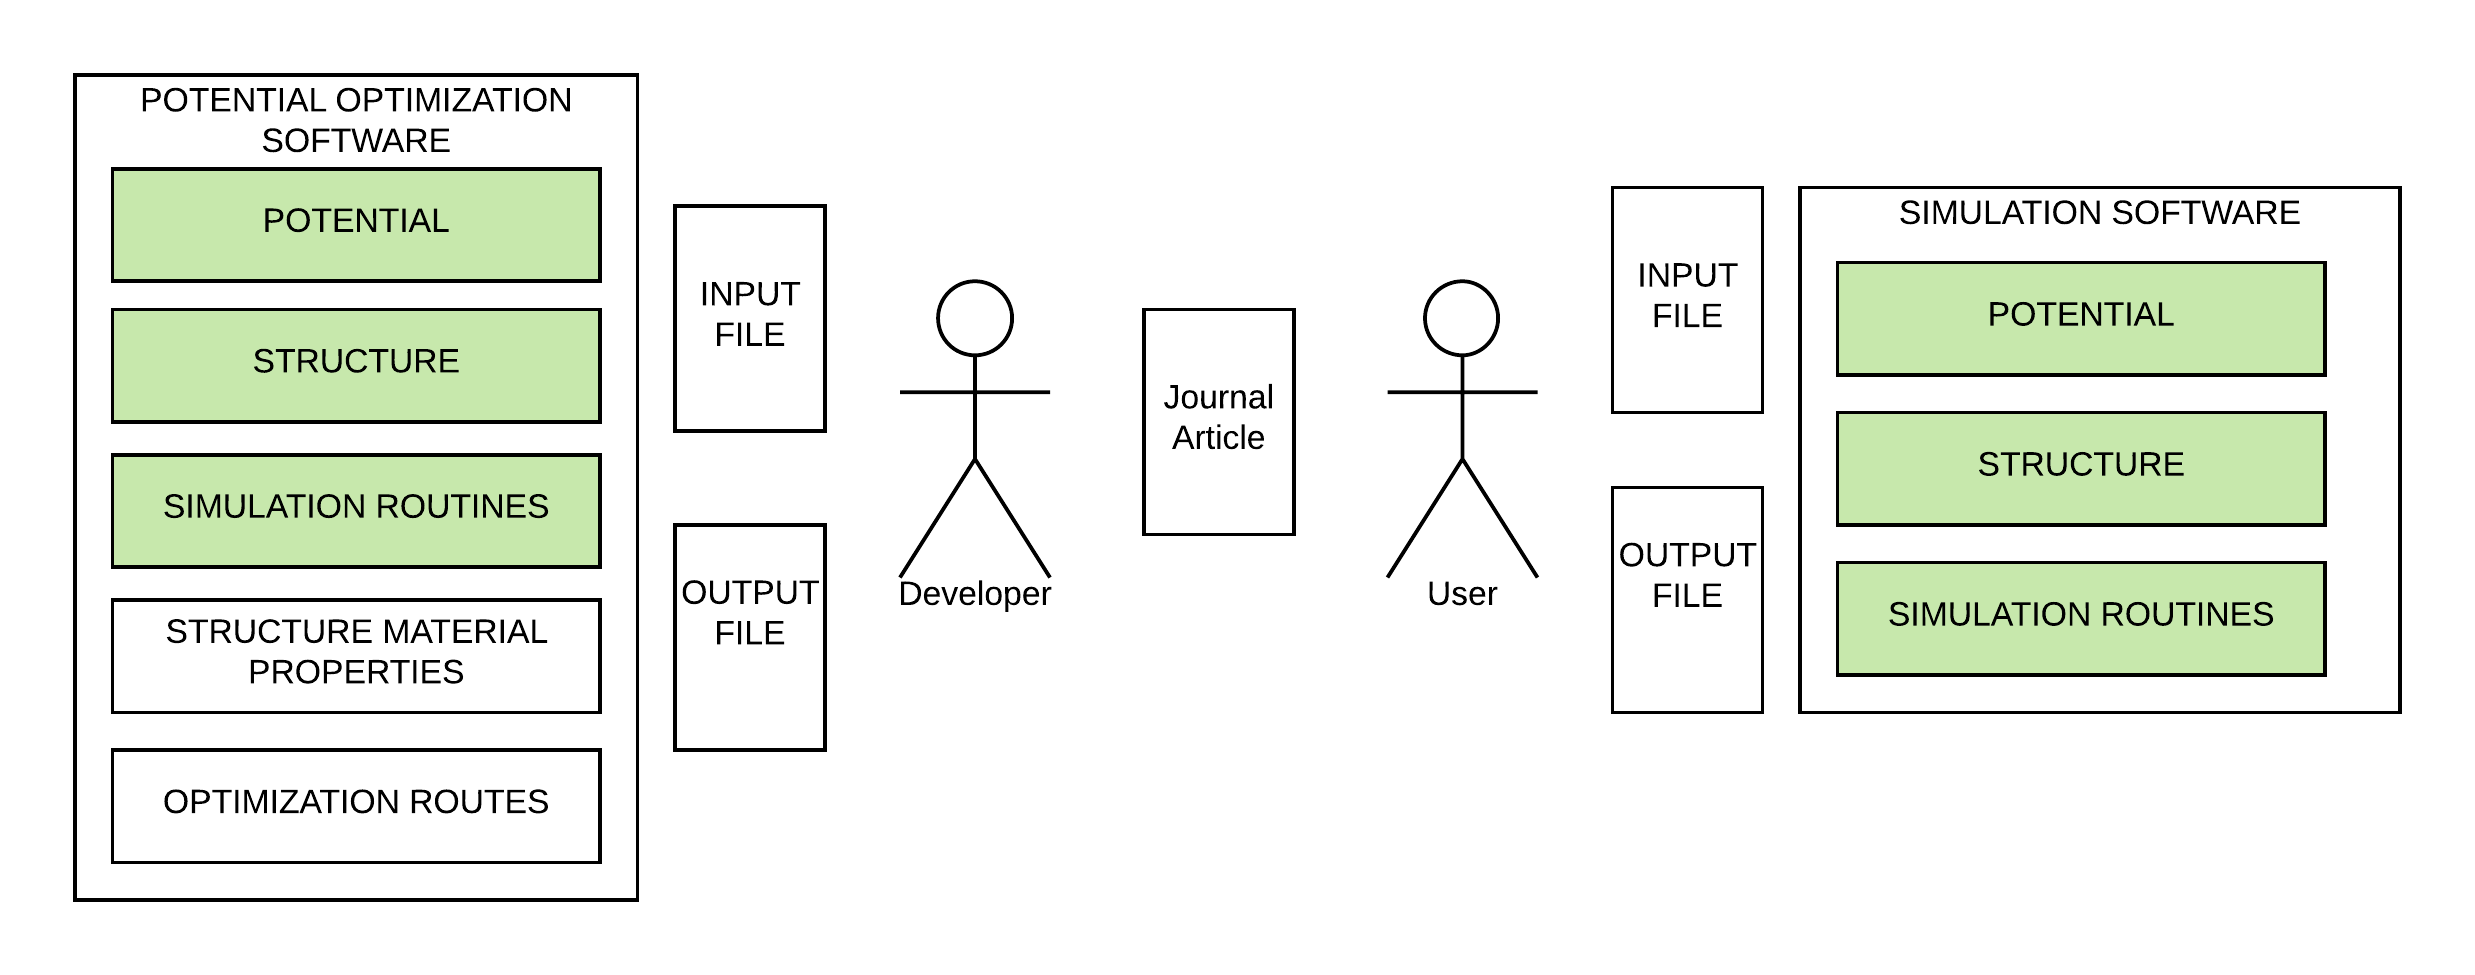
\includegraphics[width=5in]{chapter6/img/fig_potdev_monolithic}
	\caption{Schematic of monolithic potential development software}
\end{figure}

Figure \ref{fig:potdev_monolithic} is a schematic between potential development software, simulation software, the potential developer, and the potential user.  In this software architecture, The code for implementing the potential, the structures, and simulation routines common to molecular dynamics software.

Computational atomistic simulation involves software which have been developed in a variety of different languages, including but not exclusive to C/C++, and Fortran.  The combination of compiler optimization from strict variable types, well-vetted numerical libraries, and availability of parallelization libraries makes these langagues well-entrenched for the forseeable future.  The most popular atomistic simulation codes have matured over long-periods of time, with significant code contributions from the developers of potential formalisms enhancing the capabilities of the software.  For example, LAMMPS was originally written in Fortran, ported to C/C++.

Similarly, potential development software likewise developed iteratively, but with drastically different results.  Early potentials were developed using proprietary simulation codes which were augmented to describe the ability to describe the specific set of simulations to conduct required to optimize a specific set of simulations to calculate structure-property relationships.   In addition, numerical optimization routines to minimize a cost function as described in chapter \ref{ch:potential_development}.  Software codes included the ability to assign weights to the function to encode preferences and evolved to include global optimization techniques, such as simulated annealing\cite{kirkpatrick1983_simmulated_annealing} to deal with the local minima.

Despite the drastic expansion in the amount of formalisms and maturation of simulation codes, potential development software remains tailored to specific potentials and applications.  Potential software was written which support a small subset of potential formalisms.  For example, \emph{POSmat}\cite{martinez2016_posmat} supports the development of COMB potential and \emph{potfit}\cite{brommer2015_potfit} supports the development of embedded atom potentials (EAM).  On the other hand, GULP supports development of potentials based on a relatively small set of material properties.

The monolithic software development model is ill-suited for the demands of potential development.  As indicated in Figure \ref{fig:potdev_monolithic}, the regions in green represents a replication in development effort with simulation codes.  The implementation, maintenance, and updating of molecular dynamics code is non-trivial.  This effort is duplicated and better implemented in widely-adopted software codes such as LAMMPS.  More importantly,  there is little incentive for a third-parties to implement new potential formalism to monolithic software development codes.

Discussed in depth in chapter \ref{ch:potential_development}, the final parameterization on depends choices made by the potential developer; this means that the process by which a potential is developed is generally neither fully documented, nor reproducible.  Moreover, there is currently no objective method for evaluating the suitability of the function form of the atomic potential or determining if the final parameterization selected yields the best possible fit to the fitting database.  Current parameterization processes generally involve the minimization of a single scalar cost function, typically a weight sum of some measure of the predicted value, $\hat{q}_i(\bm{\theta})$ and the reference values of the specific material property $\hat{q}_i$.

As a result, the final parameterization depends on the many choices made by the potential developer; this means that the process by which a potential is developed is generally neither fully documented, nor reproducible.  Nevertheless, the process of potential development largely remains non-transparent and subjective,\cite{martinez2013_fitting,martinez2016_posmat} involving the repeated intervention of a skilled potential developer.\cite{brenner2000_fitting}
This leads to issues to problems with reproducibility in potential development as the selection of weights and initial conditions are largely not documented with the literature.
As a result, this knowledge is largely proprietary, remains concentrated in potential development groups, and software for potential development remain rudimentary tools developed by the specific needs of potential development groups.

In addition, parameter optimization is dependent upon numerical optimization techniques indicated in orange in Figure \ref{fig:potdev_monolithic}.  As described by Ghosh and Chakraborty \cite{ghosh2014_potdev_pareto}, the general problem of parameterization is a classic problem in the application of black box functions.  Cost function optimization techniques are unable to obtain compromise solutions which are Pareto efficient, but are occluded within a convex region of performance space.

\subsection{Goals of this Software}

Software for potential software development is by necessity a complicated piece of software which draws expertise from many disciplines for software development.

The goal of pypospack is to provide a software with a flexible software architectural library from which potential developers can quickly create their own potential optimziation software, by leveraging an object-orient software framework based upon a series of core packages, which deliver specific functionality to \emph{pypospack}.

\subsubsection{Ease of Development}
The targeted audience of \emph{pypospack} is a potential developer would this software package to parameterize ther own potentials using an existing formalism by modifying the existing examples distributed with this program.

In this case, the functional form of interest is already implemented in an external simulation code, but not implemented in \emph{pypospack}.  A goal of \emph{pypospack} is minimize the time spend in software development, so the potential spends more time in simulation and analysis of candidate potentials.

Ease of development is primary concern, computational efficiency is the secondary concern.
Rather than searching for computational efficiency by making \emph{pypospack} more monolithic, the design decision should instead prefer to leverage existing capability of external simulation codes.

Software for potential development is by necessity complicated.  The topic is technical requiring an understanding in doing computational simulations, combining these simulations to calculate material properties, then applying numerical analysis techniques to create candidate potentials.

The monolithic nature of existing potential optimization codes make code contribution difficult, because few people have the requisite expertise to understand all the implementation details in the code.

To break the problems of monolithic software development, \emph{pypospack} implements an object-oriented framework with extensive use of base classes to encapsulate implementation.  \emph{pypospack} decomposes the problem so that new functionality is focused on developing new code, rather than modifying existing code.  Additionally, since new functionality subclasses the base classes, any improvements in the computational efficiency or accuracy of either the base class or an encapsulated class improves the performance of contributed code as well.

\subsubsection{Scalability}

\emph{pypospack} should not only scale to use HPC asssets, but most components should be sufficiently lightweight so that development, testing, and analysis can be done on a personal workstation

In its primary use, the potential developer approximates the set of parameters  which produces Pareto optimal predictions, $\bm{\Theta}^*$.
In the process described in Chapter \ref{ch:methodology}, the space containing parameters, $\bm{\theta} \in \bm{\Theta}$, is sampled from a probability distribution, $\bm{\theta}(\omega) \in \bm{\Theta}(\Omega)$.
Many of the potentials evaluated will be non-optimal and converging of probability distributions from the initial distribution to the final distribution is slow.

To ameliorate this computational issue, \emph{pypospack} should be written to support different concurrency schemes.  \emph{pypospack} objects should be written to easily support serialization and deserialization, so that concurrency can be implemented through messaging passing technologies.

At the same time, it is important that \emph{pypospack} runs on workstations.  First, modern development is usually iterative and focuses on the implementation and testing of classes and methods.  A minimal amount of classes should be MPI-aware, parallelization code is notoriously difficult to test.
In modern data analysis processes, data analysis is interactive.  Configuration files and data files should be easily serializable to make interactive data analysis more accessible.
In support of this goal, \emph{pypospack} is implemented in Python which has strong support for interactive execution environments.  Large amounts of data are stored natively in popular data analysis frameworks.

\subsubsection{Flexibility}

\emph{pypospack} delivers a software library with a flexible architecure library.  From these components, applications for potential optimization and potential analysis should be able to developed quickly.  This should enable potential developers to tailor potential optimization software for their own needs.

Like other potential development software packages, \emph{pypospack} was developed to seprate the process of parameter optimization from the selection of the analytical form of the potental.  \emph{pypospack} separates itself from other packages by designed using object-oriented methods which enables users of this software to quickly implement potentials supported by external codes, calculate new material properties, and even replace the optimization techniques.

Despite the technical nature of the process, the process of potential development has a variety of decisions in the choice of material properties to optimize .  In addition, since empirical potentials are approximation of the potential energy surface, the potential selection is a value judgement, dependent upon the experience and skill of the potential developer.

The key driver of this software is to implement a systematic methodology to fit interatomic potentials that allows the objective evaluation of the quality of the parameterization, and the stability of the functional form, and that is both completely algorithmic and reproducible.

\subsubsection{Extensibility}

Likewise, this software has a functional requirement to explore issues regarding parametric uncertainty of interatomic potentials described by analytic functional forms.
This topic is very broad which includes the topic of multi-objective optimization, uncertainty quantification of predicted material properties propogated from uncertainty in the empirical potential's parameters, and the application of machine-learning techniques.
All these topics are active areas of research drawing interest from multiple-disciplines.  The \verb|pypospack| framework should likewise be flexible to quickly enable the implementation new algorithms and approaches toward this problem.

More generally, the secondary goal of this software project is to implement the necessary architecture for potential developers to write their own potential development software, either by extending the base the class to include more potential formalisms, simulations tasks, and calculation of material properties.  As a result, specific software architecture decisions were made to decouple the base classes from each other.

In general, this software focuses on the integration of other software.  It interacts with other software packages, but is loosely coupled by encapsulating interation of that software through an integration layer of objects.

In this way, it is possible to change the third party software dependencies by the implementation of a new integration layer.  Despite this loose coupling, great care was taken to ensure the selection of prominent softwre packages.  The benefits of using widely-accepted existing software include avoiding the mistakes involved from self-implementation, saving development effort, and that the underlying routines have sufficient documentation and support.


\subsection{Structure of this chapter}

This chapter starts by first discussing architectural considerations taken into account in the development of this software library.  Section \ref{sec:software_architecture} includes language selection, incorporation of prominent software packages, and core design choices which has implication for the use of this software package.  At the heart of the problem is the implementation of potentials, structures, and material properties which are described first.

Section \ref{sec:potential_evalaution} deals with the generalizing the calculation of material properties.  The calculation of material properties is often decomposed into several different simulations, the simulations executed, and the results gathered.  With the results from the individual components calculated, the material property of interest can then be calculated.  This section describes how this model decomposition is implemented and the execution framework evaluating a single parameter.

Both of these sections implements concepts introduced in Chapter \ref{ch:potential_development} and reuses the notation.  With the evaluation of a single parameter set accomplished, Section \ref{sec:software_sampling_strategies} describes implementation of the evolutionary strategy described in Chapter \ref{ch:methodology}.  In addition, to a discussion of the types of strategies implemented, this section specfically discusses how computational scalability is achieved by resolving concurrency and parallelization issues to ineable this software's use in high-performance computing environments.

While older monolithic codes have terse input and output files, the issues of accessibility to software in \emph{PyPOSPack} are resolved through the concept of object serialization and deserialization.  Section \ref{sec:softwre_acessibility} describes this strategy.  Since every object in \emph{PyPOSpack} can be instanced by a dictionary datastructure, the definition of an optimization process can be represented as a nested list of dictionaries.  This enables potential developers to define evolutionary strategies quite compactly, since the the deserialization results of the previous interation are used to serialized the next iteration.

Section \ref{sec:software_analysis}, we demonstrate the power of this framework, by looking at how the large amounts of data produced by simulation methodology is readily available to potential developer using well-known data analysis tools.  With the removal of traditional input and output files, the large amounts of data generated are readily accessible and accessible for exploratory data analysis.

\section{Software Architecture}
\label{sec:software_architecture}

\subsection{Licensing}

\subsection{Programming Language}
\emph{PyPOSPack} is written in Python 3 to leverage the strength of python as a high-level language for writing scientific applications.  Python has a liberal open source license which makes the distribution of the application without license issues.  Compatability across platforms is a major design consideration.  Since Python available of a wide variety of operating systems, there are few issues with portability as \emph{PyPOSPack} is written to be platform agnostic.

\emph{PyPOSPack} utilizes prominent open-source packages from the python community.  Python is popular programming language that is popular for scientific applications, due to the maturity and stability of fundamental numerical libraries, quality of documentation, and availability of well-supported distrbutions, such as Anaconda\cite{python_anaconda}, makes Python accessible and convenient for a broad audience.  Additionally, matplotlib\cite{hunter2007_matplotlib} integrated with IPython\cite{} provides an interactive research and development environment with data visualization suitable for most users.  As a result, is an appealing choice for algorithmic development and exploratory data analysis\cite{dubois2007_python}

\subsection{Integrated Software Packages}
Since, \emph{PyPOSPack} takes a different approach to the development of potentials by identifying a set of Pareto optimal potentials through an evolutionary process.  NumPy\cite{walt2011_numpy} adds an array language, similar in syntax to MATLAB, and similar in power to Fortran, in which operations are performed in compiled code.  This package provides linear algebra capabilities through this extended interfaces to BLAS\cite{blas2002} and LAPACK\cite{anderson1990_lapack}.  Scipy\cite{jones_scipy} builds on top of NumPy to provide functionality for optimization, numerical integration, and a statistics package for creating random variates.

The python language has a clean syntax yet has sophisticated constructs which allows is indifferent to either procedural or object-oriented programming styles, as the situation dicates.  Software development for this program was developed using procedural code, which was later encapsulated to classs object to abstract the implementation details into base objects.  The success of \emph{pymatgen} in transforming the high-throughput search of materials,  where the materials properties can be predicted by solving fundamental laws of physics using quantum mechanical appoximation such as density functional theory (DFT).  This virtual testing of materials was employed to design and optimize materials \emph{in silico}.

For the purposes of data analysis, the data produced by \emph|pypospack| is exposed through Pandas\cite{mckinney2010_pandas} to simplify data management and data analysis tasks using well known syntax.
Scikit-learn\cite{pedregosa2011_sklearn} integrates a wide range of machine learning algorithms for medium-scale supervised and unsupervised problems. This package focuses on bringing machine learning to non-specialists using a general-purpose high-level language.

Scalability for \emph{pypospack} is provided through the MPI for Python(mpi4py(\cite{dalcin2005_mpi4py,dalcin2008_mpi4py} which provides bindings of the Message Passing Interface (MPI)\cite{mpi2015} standard for the Python programming language and allows the exploitation of multiple processors in an HPC environment.  This is important for ease of installation and portability, as providing libraries around Fortran code can prove challenging on various platforms.

\subsection{Supported Simulation Codes}

The success of these approaches is largely driven by epistemic uncertainty associated with DFT calculations are largely driven by the unknown functional form of the exchange correlation functional.

Contrast this to molecular dynamics, where $V(\bm{r}_{ij})$ has uncertainty in both the functional form and parameterization.  Before attacking problems with functional form,

Let us first consider, three fairly simple systems which are widely studied, where the fundamental physics are significantly different.  Metal systems are described by
\emph{metal} units, where further information can be found in the LAMMPS

\subsection{Software Design Principles}

This software package is implemented in a way to minimize the mathematical and technical requirements for contributing to this project.

In the development of \emph{pypospack} the abstract base classes has been refactored many times as to encapsulate as much technical implementation into base objects as possible.  The base class objects encapsulates the run-time execution details.  As a result, the development of new classes to model to potential formalisms, simulation cells, simulation tasks, and the calculate material properties, can be developed with minimal effort.  If the material properties can be calculated using results from reference LAMMPS scripts with a rudimentary understanding of object-oriented programming and Python programming competence.

Since every implemented class in \emph{pypospack} is inherited from a base class, to develop a new subclass the appropriate the base class, the necessary methods required to be overidden are defined by a method signature, which by default generates a \verb|NotImplementedError|, if the functionality is required but not implemented.

A subclass which implements all the necessary features of a base class is referred to as an \emph{implemented class}.  A subclass which does not implement all the necessary features of a base class is a \emph{derived base class}.  In the \verb|potential| package, the \verb|PairPotential| is a derived base class because  it does not implement all the method required by the \verb|Potential| class.  However, it does define methods which encapsulates implementation details which are used for implemented pair potentials such as \verb|BuckinghamPotential|.

For example, classes which implement an empirical potential formalism are all subclasses of the \verb|Potential| base class.  The \verb|write_lammps_potential_section(filename)| method signature is constant across all subclasses and does not need to be implemented.
Instead, \verb|lammps_potential_section_to_string()| method needs to be overriden and returns the string variable required in the LAMMPS input file, which is used by \verb|write_lammps_potential_section(filename)|.
Here, the subclass inherits the \emph{specification} of the method \verb|lammps_potential_section_to_string| the details of the implementation are needed.  In constrast, the subclass inherits the \emph{implementation}  of \verb|write_lammps_potential_section| abstract class.
Here the disk output implementation is encapsulated in the base class, and the potential developer is not concerned about integrating this new class into the existing code base, other than their implemented methods produce the required behavior.
This software architecture approach makes code development for \emph{pypospack} less intimidating since the more difficult implementation details have encapsulated within the base classes.

Each implemented class is required to implement certain static variables.  For example, every implemented \verb|PairPotential| class, is required to provide a unique the static string \verb|potential_type_id| and \verb|pair_parameter_names|.  This enables code introspection, the ability of \emph{pypospack} to examine its own classes.  As a result, new functionality only requires its implementation in a new file, place it in the correct subpackage directory, and \emph{pypospack}'s introspection code will automatically integrate it into the application.

Due to the complexity of these classes, all classes have usually simple constructors, requiring only minimal information required for instantiation, compared to other workflow projects such as \emph{pymatgen}.  This design decision in intentional.  Within this software library class instantiation, class configuration, and class execution are intentionally decoupled in the base classes.  By keeping class instantiation simple, the base classes from being brittle.  If abstract classes are tightly coupled to a small set of use cases, then the abstract class is described as brittle when new use cases are unable to reuse either the specification or implementation of a base class.  As \emph{pypospack} is designed to accomodate a wide variety of potential formalisms, simulation tasks, and material properties, classes within \emph{pypospack} are designed to be as general as possible.

To specialize subclasses for more specialized purposes, configuration of objects are done after class initialization by passing dictionaries into methods.  Every object within \emph{pypospack} can initialized and configured by dictionary initializtion.  Known more generally as a hashtable, these collections of key-value pairs are implemented in Python as a data structure called a dictionary (i.e. \verb|dict| or \verb|OrderedDict|).
  Since method specification is generalized, it is easier to encapsulate dozens of different classe representing potentials, simulations tasks, and material properties, without requiring the implementation of specific \emph{if}-\emph{else if}-\emph{else} idiomatic expressions, which must be rewritten every time new functionality is added to \emph{pypospack}

Since dictionaries are used for initialization, \emph{pypospack} makes extensive use of object serialization, by encapsulating pertinent information into a data structure of key-value pairs.
The implementation of the dictionary constructor has the benefit of providing object serialization from strings.  PyPOSPack implements YAML("YAML Ain't Markup Language")\cite{yaml_version_1_2r} object serialization as a compromise between XML ("eXtensible Markup Language") and the definition of their schemas and JSON ("JavaScript Object Notation").  These three file format have prominent existing libraries, which prevents mistakes which can occur from implementing file parsers
One problem with potential development software are system integration issues involving the creation of input files and parsing of output files.

The currently implemented classes have straight forward implementations, well-documented, and provide templates to encourage others to contribute to the \emph{pypospack} software.

\subsection{Potential Formalisms}

The software development effort associated with developing new potentials for potential optimization software is typically time-consuming, requiring the implementation not only of the potential $\hat{V}$ but also the implementation of the second-derivatives with respect to changes in interatomic positions to computational issues with numerical approximation.  In \emph{PyPOSPack}, this requirement has already been implemented by the simulation software, which drastically reduces the software development time to implement existing formalisms already supported by either LAMMPS or GULP.

The \verb|potential| package contains class objects which inherit from the appropriate abstract base class and overide the required methods for implementation.  The \verb|Potential| abstract class only expects implementation of the \verb|_init_parameter_names|, \verb|lammps_potential_section_to_string|, \verb|gulp_potential_section_to_string|, \verb|lammps_parameter_file_to_string| and \verb|evaluate| methods.  However, not each method needs to be implemented.

Depending upon the use of the potential, not all methods need to be overridden.  For example, if simuations are only run in LAMMPS, then the only the \verb|lammps_potential_section_to_string| would need to be implemented to be implemented respectively.

Likewise, some implemented \verb|Potential| classes are not implemented in LAMMPS or GULP and are used in the composition of tabulated values.  In these cases, only the \verb|evaluate| method is required to be implemented.

In \emph{PyPOSPack}, the \verb|potential| package contains classs objects, which inherit from methods from the appropriate base class.  The base classes have been implemented in \verb|potential|: (1) \verb|PairPotential|, (2) \verb|ThreeBodyPotential|, (3) \verb|EamDensityFunction|, and (4) \verb|EamEmbeddingFunction|.
\subsubsection{PairPotential}

In \emph{pypospack} applications, a potential formalism is defined by specifying the \verb|potential_type| and the \verb|symbols| as an dictionary object:
\begin{lstlisting}[language=Python]
potential_formalism = OrderedDict()
potential_formalism['potential_type'] = 'buckingham'
potential_formalism['symbols'] = ['Mg','O']
\end{lstlisting}

The \verb|PairPotential| implements a standard potential naming scheme.  As a result, it is necessary only to define the \verb|pair_parameter_names| attribute in implemented potential classes.  For example, for a pair potential with a parameter, $A_{Mg,O}$, satifies the $A$ parameter of the Mg-O pair potential term, and would have the name \verb|MgO_A|.  The recommended convention for naming parameters is to prefer the same variable naming convention scheme listed in LAMMPS documentation, then the variable naming scheme listed in original literature.

To evaluate a specific potential the parameter set must be defined as a dictionary object.  For example, as part of a collection of reference potentials, the dictionary object containing the original parameterization is
\begin{lstlisting}[language=Python]
reference_potentials['SW'] = OrderedDict([
    ('SiSiSi_epsilon',2.1686),
    ('SiSiSi_sigma',2.0951),
    ('SiSiSi_a',1.80),
    ('SiSiSi_lambda',21.0),
    ('SiSiSi_gamma',1.20),
    ('SiSiSi_costheta0',-1/3),
    ('SiSiSi_A',7.049556277),
    ('SiSiSi_B',0.6022245584),
    ('SiSiSi_p',4.0),
    ('SiSiSi_q',0.0),
    ('SiSiSi_tol',0.0)
])
\end{lstlisting}

Implemented pair potentials are indicated in Table \ref{tbl:pypospack_pair_potential}.

\begin{table}[ht]
    \centering
    \caption{Implemented pair potentials in \emph{PyPOSPack}.}
    \label{tbl:pypospack_pair_potential}
    \begin{tabular}{ccccc}
	    \hline
	    {Class Name} & LAMMPS & GULP & EAM  & {Reference} \\
	    \hline
	    BuckinghamPotential   &   &   & x & \cite{lewis1985_buckingham,buckingham1938} \\
	    MorsePotential        & x & x & x & \cite{morse1929_morse_potential} \\
	    BornMayerPotential    &   &   & x & \cite{abrahamson1969_bornmayer_potential} \\
	    LennardJonesPotential & x & x & x & \cite{lennardjones1924_lj_pot} \\
	    GeneralizedLennardJonesPotential
	                          &   &   & x & \cite{mishin2004_eam_NiAl} \\
	    \hline
    \end{tabular}
\end{table}

\subsubsection{Three Body Potentials}
Three body potentials are implemented in with the base class \verb|ThreeBodyPotential|, and listed in Table \ref{tbl:pypospack_threebody_potentials}.  Unlike pair-potentials, the potential naming schemes are not equivalent.

In the Stillinger-Weber potential\cite{stillinger1985_sw}, a pair potential term $V_2(r_{ij})$ is dependent upon the interatomic separation distance between atoms $r_{ij}$ between atoms $i$ and $j$.
To model angular dependence the three-body term $V_3(r_{ij},r_{ik},\theta_{ijk})$ augments the $V_2$ term, where $i$ is the central atom in a three body interaction.  In a Stillinger-Weber potential, an entry for \verb|SiSiC| and \verb|SiCSi| are identical since \verb|Si| is the same.

In comparison, the Tersoff potential\cite{tersoff1988_tersoff} is a pair interaction term describing the bonding of atoms $i$ and $j$ influenced by the presence by a third atom $j$.
In the Tersoff potential, an entry for \verb|SiCC| means that a silicon atom is bonded to a carbon atom and influenced by a third atom.  The three-body parameters for \verb|SiCC| and \verb|SiSiC| are not necessarily the same.  As a result, \verb|_init_parameter_names| has different implementations for three-body potentials, and the base class has not default implementation.

\begin{table}[ht]
	\centering
	\caption{Implemented three-body potentials.}
	\label{tbl:pypospack_threebody_potentials}
	\begin{tabular}{cccc}
		\hline
		{Class Name} & LAMMPS & GULP & Reference \\
		\hline
		TersoffPotential & x & x & \cite{tersoff1988_tersoff} \\
		StillingerWeberPotential & x & x &\cite{stillinger1985_sw} \\
		\hline
	\end{tabular}
\end{table}

\subsubsection{EAM Potentials}

The formalism of the EAM potential is composed of three functions: (1) a pair potential, (2) an electron density function, and (3) an embedding energy function which is dependent upon individual contributions defined by the electron density function.
The implementation of the \verb|EamPotential| class encasulates a \verb|PairPotential|, a \verb|EamEmbeddingFunction|, and a \verb|EamDensityFunction|.

  A density function $\bar{\rho}(r_{ij})$ is the electron density contribution of atom $j$ to the total electron density at the site for atom $i$.  Like a pair potentia, it is a function the interatomic separation distance.  However, each species is bound to an electron density function.  For an EAM potential with two chemical species, there are two electron density functions.  Thus the parameter naming convention would be \verb|{symbol_1}_{parameter_name}|.
	The list of implemented EAM density functions are listed in Tables \ref{pypospack_eam_density_function}.

\begin{table}[ht]
	\centering
	\caption{Implemented EAM density functions}
	\begin{tabular}{cc}
		\hline
		{Class Name} & {Reference} \\
		\hline
		ExponentialDensityFunction & \\
		Mishin2004DensityFunction & \cite{mishin2004_eam_NiAl} \\
		\hline
	\end{tabular}{cc}
\end{table}

An energy embedding function, $F(\bar{rho}_i)$, calculates the energy required to embed atom $i$ based upon electron density at the site.  Like the EAM density function, the embedding function is defined for each chemical species and has a similar naming convention for its parameters.
\emph{pypospack} supports two representations of the embedding function.
The default implementation defines the embedding function, $F(\bar{\rho}|\bm{\theta})$, as regular analytical function.

The second representation comes from determing the embedding function implied by the equation of state, a technique pioneered by Foiles \emph{et al.}\cite{foiles1986_eam_embedded_eos}.
The \verb|EamEmbeddingEquationOfState| provides a base class for the numerical estimation of these functions, and are listed in Table \ref{tbl:pypospack_eos_embedding_function}.
Although not typically included in the definition of the parameter set, a string variable specifying host lattice (e.g. fcc, bcc, hcp) of the ground state, \verb|lattice_type|, as well as the lattice parameter, $a_0$ are necessary.

\begin{table}[ht]
	\centering
	\caption{Implemented Analytical embedded energy function.}
	\label{tbl:pypospack_embedding_function}
	\begin{tabular}{cc}
		\hline
		{Class Name} & Reference \\
		\hline
		BjsEmbeddingFunction & \\
		UniversalEmbeddingFunction & \\
		FinnisSinclairEmbeddingFunction & \\
		\hline
	\end{tabular}
\end{table}

EAM potentials are not defined in simulation software as analytical potentials, but provided in a pre-calculated tabulated the \emph{setfl} format.  The class \verb|SetflFile| contained in the \verb|eamtools| packages deserializes a parameterized EAM potential into the expected format.

\begin{table}[ht]
	\centering
	\caption{Implemented EAM embedding function determined from the inverse equation of state}
	\label{tbl:pypospack_eos_embedding_function}
	\begin{tabular}{cc}
		\hline
		{Class Name} & {Reference} \\
		\hline
		RoseEosEmbeddingFunction & \cite{foiles1984_eam_eos} \\
		ZopeMishinEosEmbeddingFunction & \cite{zope2003_eam_eos} \\
		\hline
	\end{tabular}
\end{table}

To define an EAM potential, it only necessary to specify the chemical species, and the formalism of the pair, density, and embedding function.
\begin{lstlisting}[language=Python]
	potential_formalism = OrderedDict()
	potential_formalism['potential_type'] = 'eam'
	potential_formalism['symbols'] = ['Ni']
	potential_formalism['setfl_filename'] = None
	potential_formalism['pair_type'] = 'bornmayer'
	potential_formalism['density_type'] = 'eam_dens_exp'
	potential_formalism['embedding_type'] = 'eam_embed_eos_rose'
\end{lstlisting}

\subsection{Structural Representation}
\label{sec:pypospack_structures}

The representation of a structure was formalized in Section \ref{sec:configuration_space}, but impose certain restrictions to communicate information on about the unit cell, and ensure that geometry is compatible with LAMMPS.
The lattice vectors of a simulation cell are embedded in Euclidean space,  $\bm{a}_i = [a_{11}, a_{12}, a_{13}] \in \mathbb{R}^3$ for $i \in [1,2,3]$.  To ensure that the crystal structure can be defined in LAMMPS, we impose restructions defined by the following matrix representation:
\begin{equation}
	\begin{bmatrix}
		a_{11} & a_{12} & a_{13} \\
		a_{21} & a_{22} & a_{23} \\
		a_{31} & a_{32} & a_{33}
	\end{bmatrix}
	=
	\begin{bmatrix}
		\ell_x    & 0         & 0     \\
		\tau_{xy} & \ell_y    & 0     \\
		\tau_{xz} & \tau_{yz} & \ell_z
	\end{bmatrix}
\end{equation}
Here $\ell_x$, $\ell_y$, $\ell_z$ define a length of parallelpiped unit in the orthogonal $\hat{u}_x$, $\hat{u}_y$, and $\hat{u}_z$ directions with $\tau_{xy}$, $\tau_{xz}$, and $\tau_{yz}$ representing how much the parallelpiped is tilted from the orthogonal axis.

For a unit cell, the magnitude of the lattice vectors $\bm{a}_1$, $\bm{a}_2$, and $\bm{a}_3$ correspond to the $a$,  $b$, and $c$ from the typical crystallographic representation of a unit cell.  In order to encode this information, each $\bm{a}_i$ is normalized by transforming $\bm{a}_1$ unto a unit vector by its length $a_0$.  For a cubic system, the matrix representation now becomes
\begin{equation}
\label{eq:pypospack_lattice_vector}
	\begin{bmatrix}
		a & 0 & 0 \\
		0 & b & 0 \\
		0 & 0 & c
	\end{bmatrix}
	=
	a_0
	\begin{bmatrix}
		1 & 0 & 0 \\
		0 & \frac{b}{a} & 0 \\
		0 & 0 & \frac{c}{a}
	\end{bmatrix}
	=
	a_0 \begin{bmatrix}
				\bm{h}_1 \\
				\bm{h}_2 \\
				\bm{h}_3
			\end{bmatrix}
	=
	a_0 \bm{H}
\end{equation}

To represent a supercell $n_1 \times n_2 \times n_3$, the modified $\bm{H}$ matrix then becomes
\begin{equation}
\label{eq:pypospack_supercell_representation}
	a_0 \bm{H}'
	=
	a_0 \begin{bmatrix}
	        n_1 \bm{h}_1 \\
					n_2 \bm{h}_2 \\
					n_3 \bm{h}_3
			\end{bmatrix}.
\end{equation}

Representations of crystal structures is implemented in the package \verb|crystal|.  The base class for all crystal structures is \verb|SimulationCell|.  Representation of the lattice vector is set by determining Equation \ref{eq:pypospack_lattice_vector}, by setting the attribute values \verb|a_0| and \verb|H|, where \verb|H| is a $3 \times 3$ matrix stored as a \verb|numpy.ndarray|.  The \verb|atomic_basis| attribute is a \verb|list| of \verb|crystal.Atom| objects which store in addition to the position $\bm{r}$, the chemical species $\alpha$, and a variety of optional \verb|None| assigned attributes which can be assigned to represent physical quantities such as charge and magnetic moment.  A number of optional convenience methods and factory functions, such as getting the number of atoms of each chemical species are represented, creating supercells, and adding/removal of atoms to point defects.

For intercompatibility with the VASP file format for structures, \verb|io.vasp.Poscar| is a subclass. \verb|SimulationCell|.  This class can read and write POSCAR formatted files through the implemented \verb|read()| aand \verb|write()| methods.
To interact with LAMMPS has likewise been created in \verb|io.lammps.LammpsStructureFile| object through the \verb|io.gulp.get_structure_string()| and \verb|write()| methods
Access to the tools to create orthogonal cells from hexagonal lattices and provide different orientations of the lattice is automated through integration of the Atomic Simulation Environment (ASE)\cite{larsen2017_ase}.

The creation of a structure database is defined by class \verb|StructureDatabase|.  The structure database has two important attributes consisting of a \verb|path| attribute variable which contains the path to the directory containing all the structures.  For each structure, one needs to provide the \verb|filename| of the structure file and a unique string which serves as the key value to identify the structure.  Examples contained within the \verb|pypospack| distribution, use the chemical composition, the crystal structure, and the type of crystal structure.  For example, a representative FCC unit cell of nickel would be referred to by \verb|Ni_fcc_unit|.

The creation of structure files is often one of the more challenging processes for someone new to computational materials science.  To aid in the creation of a structure database, a variety of convenience classes and factory methods help automate the instantiation of these objects, identity points where interstitial defects can be inserted, orient crystals to common miller index locatations, create slabs for surface calculations, reciprocal space lattice vector, and get $k$-point paths for bandwidth calculations.  Currently, this functionality is implemented for face centered cubic, $\alpha$-quartz, diamond cubic, and rocksalt crystals.

\section{Modelling and Execution Framework}
\label{sec:potential_evalaution}

At this point, the discussion moves to the fundamental functionality, which automates a set of material properties for a given functional form for a variety of parameters.  Since one of the goals of this software package framework is to provide a lightweight modelling framework, which encapsulates implementation details within abstract classes.

Unlike \emph{ab initio} DFT automation frameworks which conducts a simulation for permutations of a structure in search for an optimal material.  Each calculation here is expensive, requiring tens of minutes or even hours of simulation per calculation.  Here we have a smaller number of structures, which remain fixed while we iterate over a large number of calculations which take a short amount of time.  As a result, the engine to manage the workflow is much different.

This section first with a discussion of a modelling workflow for the calculation of material properties, by going through the process of automating the defect formation energy.

\subsection{Modeling Framework}

To run simulations, \emph{pypospack} spawns a new process, through the Python \verb|subprocess| module, and obtain the exit codes, which is returned from the child process and is interpreted by \verb|pypospack| in the event of external codes returning a success or failure.  Through this facility, input files are made for the external executable, which is run under a child subprocess until an exit code is detected, when the output files of the energy calculator are then parsed for pertinent information.  Currently, \verb|pypospack| supports LAMMPS, GULP, VASP as external energy calculators.  The VASP functionality is not fully featured and exists to promote consistency in the calculation of \emph{ab initio} reference values $\bm{q}$.

The choice to use an external energy calculator rather than implementing one internally was chosen to eliminate the maintenance of simulation software and implementation of potential formalisms.  Even for potential developers who create new functional forms, code design, implementation, and maintenance is limited to their code code contributions in LAMMPS.
While an application programming interface (API) to LAMMPS does exist, \emph{pypospack} implements the calculation of material properties through input and output files is a practical necessity.  Computational materials scientists already have existing LAMMPS scripts which are reused for compute a variety of material science properties.  Using a "process determines software design" approach, an approach for the automation of material properties is now presented.

To demonstrate the ability of this framework to quickly automate the calculation of material properties, the process for the automation of a point defect calculation is demonstrated.

\begin{figure}[ht]
	\label{fig_point_defect_calculation}
	\centering
	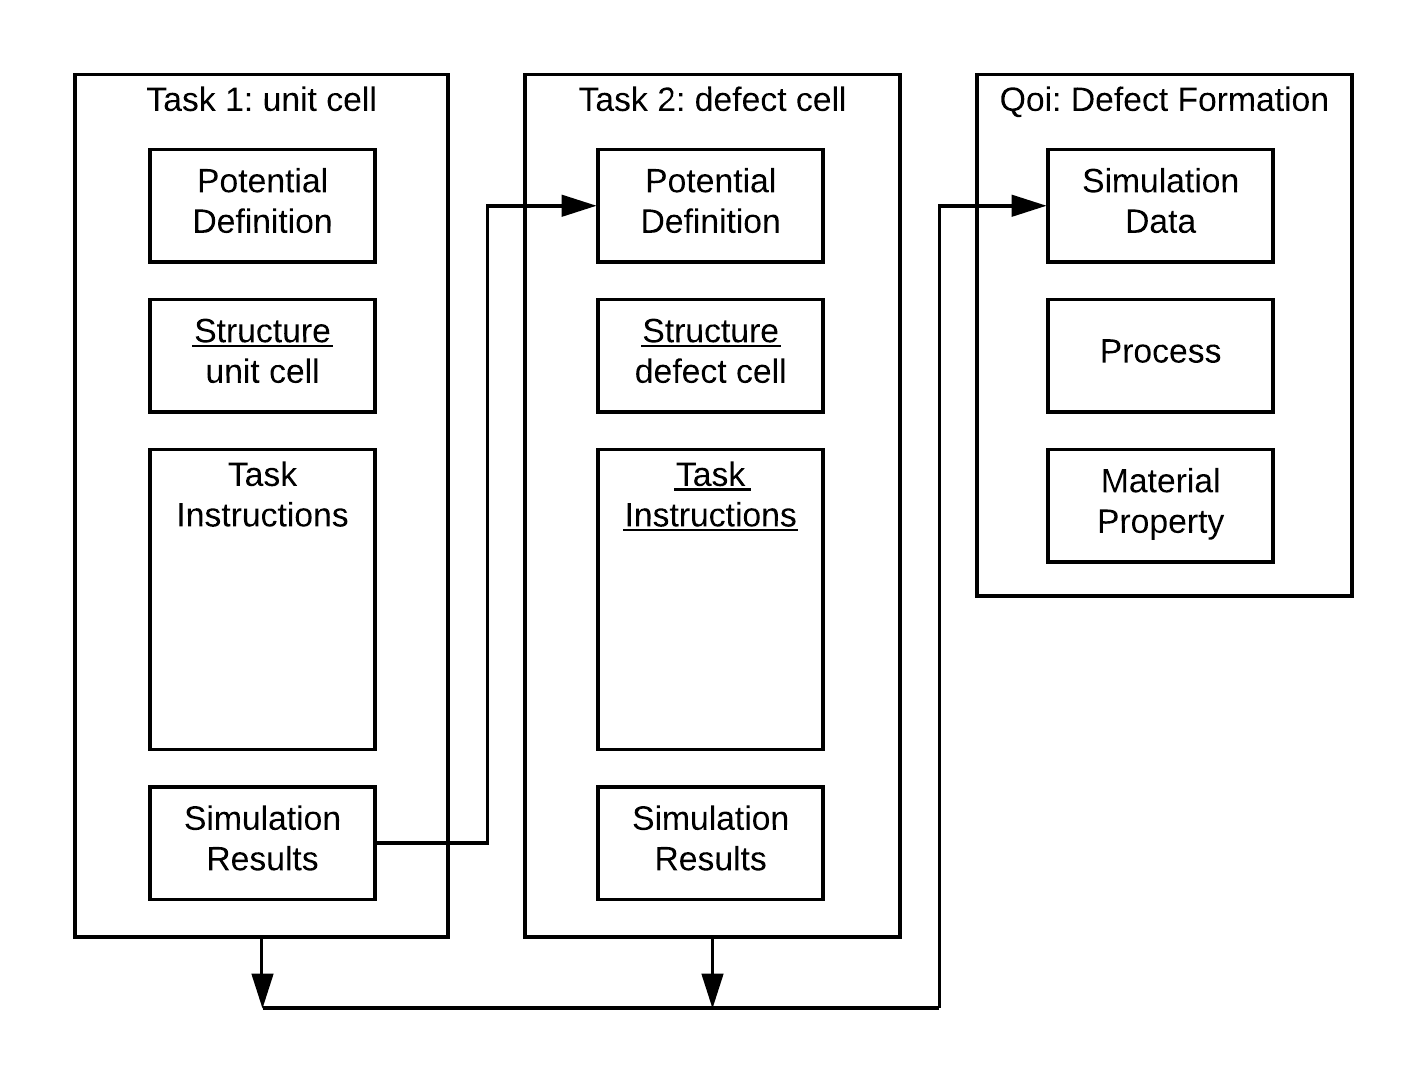
\includegraphics[width=5in]{chapter6/img/fig_point_defect}
	\caption{Schematic of for the calculation of point defect calculations.}
\end{figure}

In the first step of the automation process, a potential developer first creates a set of reference simulations required to calculate a material property.  Figure \ref{fig_point_defect_calculation} provides a schematic of various components involved in the calculation of a quantity of interest using the supercell method.  In this case, it starts at a series of LAMMPS or GULP scripts, with the calculation of the material property done with a commercial spreadsheet calculations.

\subsubsection{Simulation Tasks}

In \emph{pypospack}, the execution of simulation tasks are subclasses of \verb|Task| class.  The derived base classes \verb|LammpsTask| and \verb|GulpTask|, provides the necessary methods for implementing LAMMPS and GULP simulations. \verb|Task| objects are primarily responsible for managing the input and output files for simulation against an external code.  In the expected use of these classes for parameter optimization, external simulation are run a subprocess to a \emph{pypospack} application, and derived base classes are reponsible for managing these subprocesses.

In the case of LAMMPS simulations, the simulation scripts consists of four sections:  the potential definition, the structure definition, instructions to calculate the required simulation, and an output section.  GULP input scripts are decomposed in a similar way.

 This class encapsulates the \verb|Potential| class and the \verb|SimulationCell| class.  As a result, to implement a \verb|Task| class requires three steps: (1) defining of LAMMPS instructions, (2) parsing the output file to retreive the results of the simulation, and (3) populate the \verb|task_results| dictionary with the results.  The first step is already completed in the reference LAMMPS script; the other two steps are rudimentary programming tasks.

The calculation of the Figure \ref{fig_point_defect_calculation} shows material property requires two simulations.  The first simulation involves one involving the minimization of a unit cell representing an ideal bulk structure.  In this simulation, a simulation process known as structural and position relaxation is conducted.  Here, the minimum energy basin is attains by either steepest descent or conjugate gradient method of minimizing the energy with respect to the atomic positions of each atom, the volume of the simulation cell, and the shape of the supercell.  This simulation provides the energy $E_{c,\mathrm{bulk}}$, as well as structural properties of the lowest energy atomic configuration of the phase represented by the unit cell.  This simulation type has been implemented in as \verb|LammpsStructuralMinimization| and has the \verb|task_type_id| of \verb|min_all|.

The second calculation a simulation involving a defect structure.  Here the defect is embedded into a larger supercell representation of the bulk structure.  This is necessary to prevent defect from interacting with itself across the periodic boundary conditions.  Here the shape and volume of the simulation cell is held fixed, while the conjugate gradient method minimizes the positions only.  This simulation type has been implemented in \verb|LammpsPositionMinimization| and has the \verb|task_type_id| of \verb|min_pos|.

A feature of this simulation workflow is that that running the defect calculation is dependent upon the structural properties of the of the ideal bulk system.  \emph{pypospack} solves this problem by aggregating the results of each results of each task into a dictionary object.  Each simulation task is assigned a unique \verb|task_id| which is determined by concatenation of the \verb|structure_id|, \verb|task_type_id|.  For example, if this simulation was done to calculate the vacancy formation energy of silicon, the bulk unit cell might have the name \verb|Si_dia_unit| and the defect structure \verb|Si_dia_vac|.  Then associated \verb|task_ids| would be \verb|Si_dia_unit.min_all| for the minimization of the ideal crystal structure and \verb|Si_dia_vac.min_pos| for the energy calculation of the structure containing the defect.

In the use cases encountered so far, simulations tasks are dependent upon the structural results of their associated bulk structure.  If the \verb|bulk_structure_name| attribute is set on a \verb|Task|, the class will modify the encapsulated \verb|SimulationCell| object to extract the lattice vectors from the associated structural minimization simulation.  If other dependencies are necessary, a new simulation task can be created by subclassing the \verb|LammpsTask| and implement the desired behavior using implemented existing classes as a template.

A simulation task may produce one or more values of intererst.  The simulation produces the cohesive energy $E_c$, and the lattice vectors $\bm{a}_1$, $\bm{a}_1$, and $\bm{a}_3$ of the relaxed structure.  Currently, \emph{pypospack} marshals all simulation results into a dictionary consisting of primitive data types.  As a result, components of the lattice vector $\bm{a}_1$, would have a key values of \verb|a_11|, \verb|a_12|, and \verb|a_13|.

A list of the all the simulation tasks, and a short descriptions are summarized in Table \ref{tbl:pypospack_tasks}.  All simulation task classes are derived from the  \verb|Task| base class. There are two derived base classes: \verb|LammpsTask| and \verb|GulpTask|.

\begin{table}[ht]
	\centering
	\caption{A list of the simulation tasks currently implemented in \emph{pypospack}.}
	\label{tbl:pypospack_tasks}
	\begin{tabular}{ccc}
		\hline
		\verb|task_type_id|
		& Class Name
		& Simulation Engine \\
		\hline
    \verb|min_all|
		& LammpsStructuralMinimization
		& LAMMPS
		\\
		\verb|min_pos|
		& LammpsPositionMinimization
    & LAMMPS
		\\
		\verb|min_none|
		& LammpsStaticCalculation
    & LAMMPS
		\\
		\verb|elastic|,
		& LammpsElasticCalculation
		& LAMMPS
		\\
    \verb|npt|,
		& LammpsNptSimulation
		& LAMMPS
		\\
		\verb|nvt|,
		& LammpsNvtSimulation
		& LAMMPS
		\\
    \verb|gulp_gamma_phonon|
		& GulpGammaPointPhonons
		& GULP
		\\
		\hline
	\end{tabular}
\end{table}

The execution structure for a \verb|Task| happens in stages to accomodate to modify the conditions of the simulation based on the results of other simulation.  The stages are encoded in the attribute \verb|status|.  The states a \verb|Task| listed in increasing progression: INIT, CONFIG, READY, RUNNING, POST, and FINISHED.  An additional state, ERROR, indicates when there is a problem with the simulation.  Likewise, each status has associated callback methods: \verb|on_INIT|, \verb|on_CONFIG|, \verb|on_READY|, \verb|on_RUNNING|, \verb|on_POST|, AND \verb|on_FINISHED|.  The callback methods can be overridden, but the callback argument signature cannot be changed.  This allows an external procedure to interrogate the status of a class, and then provide the necessary information to the class.

This software design has a specific purpose to support multiple \Tasks| initialized within a container such as a \verb|list| or \verb|dict|.  The tasks are monitored within a callback loop external to the \verb|Task| objects.  The callback methods of the \verb|Task| objects should be non-blocking so the thread running callback loop can continue to monitor all the simulation tasks.  While \emph{pypospack} is not multi-threaded, multiple simulations are run simulatenously per processor, since external simulation codes are run in a child subprocess forked from the \emph{pypospack} process.  The callback loop continues until all \verb|Tasks| have either reached a FINISHED or ERROR status.

When an instance of a \verb|Task| is created, the \verb|status| is set to INIT.  A simulation directory with a unique name is created to segregate the file system context of different simulations.  Since external code execution uses an input/output file strategy, it is necessary to provide a unique context to prevent filename conflict of concurrently running simulations.

The \verb|on_INIT| callback method provides either dictionary necessary to initialize a \verb|Potential| object or an existing \verb|Potential| object is passed by reference.  The secondary mechanism is used to eliminate the computational costs of tabulation of EAM potentials, which can be expensive when the embedding function is determined from inverting an equation of state.  When this task is completed, the \verb|status| attribute is changed from INIT to CONFIG.

the \verb|on_CONFIG| callback method allows the callback loop to provide information which is not available until another simulation is complete.  The results of all completed simulations are passed as a nested dictionary of simulations.  Since each \verb|Task| instance has a unique \verb|task_id|, the task processes the dictionary to identify determine the desired configuration for the simulation.  In our example, the defect calculation awaits the results of the structural relaxation calculation of the bulk system.  If the information is not possible, the \verb|status| attribute remains in the INIT state.  When all the necessary configuration information has been acquired, all the necessary input files are written to its simulation directory, and the \verb|status| attribute is changed from CONFIG to READY.

The \verb|on_READY| method encapsulates the \verb|run()| method.  The purpose of this encapsulation is to support multiple methods of task execution.  Support for serial execution of a \verb|Task| is implemented in the \verb|run()| method.  The method identified the location of the external simulation code from the operating system environment variables.  For LAMMPS, the environment variable is \verb|LAMMPS_SERIAL_BIN|.  For GULP, the environment variable is \verb|GULP_SERIAL_BIN|.  These implementation details are encapsulated in the \verb|LammpsTask| and \verb|GulpTask|.  The execution context is changed to its simulation directory, a non-blocking subprocess is created to run the external simulation code, using the Python \verb|subprocess| module to monitor the subprocess.  Some MPI environments, have a default configuration preventing a program from spawn a subprocess, but this can normally be disabled by setting the appropriate MPI environment available in the submission script.  Once the subprocess is created, the \verb|status| attribute is change from READY to RUNNING.

However, some \verb|Tasks| require MPI support such as NEB calculations.  Other simulations require parallelization in order to complete the simulations in a reasonable amount of time,  NPT and NVT molecular dynamic simulations requiring time integrations are examples.
Since \emph{pypospack} is an MPI-aware application, it is not possible for \emph{pypospack} to subprocess MPI-aware code.  In these cases, the execution of the task is responsibility of an HPC job submission manager, like \emph{pymatgen} implements.  \emph{pypospack} does not implement a persistence model for long-running simulations, but the examples to calculate material properties which are dependent upon long-running simulations is provided in the distribution.

The \verb|on_RUNNING| polls the external simulation code.  Here there are a variety of techniques used to identify a simulation failure.  First, the \verb|subprocess| module allows us to check is the application is running, exited normally, or exited with an error.  If the external simulation code, exited with an error, then the attribute \verb|status| is marked ERROR.    If the application is running, the \verb|Task| will check to see how long the simulation is running, if the total time of the simulation exceeds \verb|max_simulation_time|, a variety of process management steps are applied to kill the child process without interrupting the parent process.  If the simulation code exited normally, the attribute \verb|status| is marked POST, indicating the simulation is complete.

The \verb|on_POST| method instructs the task to parse the output files from the external simulation code and populate a dictionary containing the results of the simulation.  The attributes of the simulation both returned to the callback thread and set as the attribute value \verb|results|.  After the post-simulation activities have been completed, the \verb|status| attribute is sent to FINISHED.

This approach to software development allows contribution for other to contribute to developing \emph{pypospack}'s capabilities by developing new simulation tasks and calculation of material properties without requiring implementation of the interfering with the technical implementation.

\subsubsection{Material Properties}

The material properties is referred to more generally in the software by the term quantity of interest (QOI), a term coming from  from verification, validation, and uncertainty quantification (VVUQ) literature.
The calculation of material properties is implemented as subclasses of the \verb|Qoi| base class.

A Qoi class may implement the calculation of one or more material properties.



In writing the QOI class, it is desireable
The calculation of the Figure \ref{fig_point_defect_calculation} material property consists of two tasks.

\begin{table}[ht]
	\centering
	\caption{A list of the Qoi classes}
	\begin{tabular}{cc}
		\hline
		Name
		  & Description \\
		\hline
    GulpOptiCalculations
		   & \verb|gulp_opti_calc| \\
		StaticStructureCalculations
		   & \verb|lmps_min_none| \\
		RelaxedPositionCalculations
		   & \verb|lmps_min_pos| \\
		RelaxedStructureCalculations
		   & \verb|lmps_min_all| \\
    ElasticPropertyCalculations
		   & \verb|lmps_elastic| \\
		PhaseOrderCalculation
		   & \verb|phase_order| \\
		DefectFormationEnergy
		   & \verb|lmps_defect| \\
		SurfaceEnergyCalculation
		   & \verb|lmps_surface_energy|  \\
		StackingFaultEnergyCalculation
			 & \verb|lmps_stacking_fault| \\
		ThermalExpansion
			 & \verb|lmps_thermal_expansion| \\
		\hline
	\end{tabular}
\end{table}

\begin{table}[ht]
	\centering
	\caption{GulpOptiCalculations}
	\begin{tabular}{cc}
		\hline
		QOI name & description \\
		\hline
		\verb|Ecoh_min_all_g| \\
    \verb|a11_min_all_g| \\
	  \verb|a12_min_all_g| \\
	  \verb|a13_min_all_g| \\
    \verb|a21_min_all_g| \\
	  \verb|a22_min_all_g| \\
	  \verb|a23_min_all_g| \\
    \verb|a31_min_all_g| \\
	  \verb|a32_min_all_g| \\
	  \verb|a33_min_all_g| \\
		\hline
	\end{tabular}
\end{table}

\begin{table}[ht]
	\centering
	\caption{StaticStructureCalculations}
	\begin{tabular}{cc}
		\hline
		QOI name & description \\
		\hline
	  \verb|Ecoh_min_none|  \\
    \verb|a1_min_none|  \\
		\verb|a2_min_none|  \\
		\verb|a3_min_none|  \\
    \verb|a11_min_none|  \\
		\verb|a12_min_none|  \\
		\verb|a13_min_none|  \\
    \verb|a21_min_none|  \\
		\verb|a22_min_none|  \\
		\verb|a23_min_none|  \\
    \verb|a31_min_none|  \\
		\verb|a32_min_none|  \\
		\verb|a33_min_none|  \\
    \verb|p_11_min_none|  \\
		\verb|p_12_min_none|  \\
		\verb|p_13_min_none|  \\
    \verb|p_21_min_none|  \\
		\verb|p_22_min_none|  \\
		\verb|p_23_min_none|  \\
    \verb|p_31_min_none|  \\
		\verb|p_32_min_none|  \\
		\verb|p_33_min_none|  \\
		\hline
	\end{tabular}
\end{table}

\begin{table}[ht]
	\centering
	\caption{RelaxedPositionCalculations}
	\begin{tabular}{cc}
		\hline
		QOI name & description \\
		\hline
		\verb|Ecoh_min_pos| \\
	  \verb|a1_min_pos| \\
		\verb|a2_min_pos| \\
		\verb|a3_min_pos| \\
	  \verb|a11_min_pos| \\
		\verb|a12_min_pos| \\
		\verb|a13_min_pos| \\
	  \verb|a21_min_pos| \\
		\verb|a22_min_pos| \\
		\verb|a23_min_pos| \\
	  \verb|a31_min_pos| \\
		\verb|a32_min_pos| \\
		\verb|a33_min_pos| \\
		\hline
	\end{tabular}
\end{table}

\begin{table}[ht]
	\centering
	\caption{RelaxedStructureCalculations}
	\begin{tabular}{cc}
		\hline
		QOI name & description \\
		\hline
	  \verb|Ecoh_min_all| \\
    \verb|a1_min_all| \\
		\verb|a2_min_all| \\
		\verb|a3_min_all| \\
		\verb|a11_min_all| \\
		\verb|a12_min_all| \\
		\verb|a13_min_all| \\
		\verb|a21_min_all| \\
		\verb|a22_min_all| \\
		\verb|a23_min_all| \\
		\verb|a31_min_all| \\
		\verb|a32_min_all| \\
		\verb|a33_min_all| \\
		\hline
	\end{tabular}
\end{table}

\begin{table}[ht]
	\centering
	\caption{ElasticPropertyCalculations}
	\begin{tabular}{cc}
		\hline
		QOI name & Units &description \\
		\hline
		\verb|c11|
		  & GPa
		  & $C_{11}$ component of the elastic tensor\\
		\verb|c12|
		  & GPa
		  & $C_{12}$ component of the elastic tensor\\
		\verb|c13|
		  & GPa
		  & $C_{13}$ component of the elastic tensor \\
		\verb|c22|
		  & GPa
			& $C_{22}$ component of the elastic tensor \\
		\verb|c23| \\
		& GPa
		& $C_{23}$ component of the elastic tensor \\
		\verb|c33| \\
		& GPa
		& $C_{22}$ component of the elastic tensor \\
		\verb|c33| \\
		& GPa
		& $C_{44}$ component of the elastic tensor \\
		\verb|c55| \\
		& GPa
		& $C_{55}$ component of the elastic tensor \\
		\verb|c66| \\
		& GPa
		& $C_{66}$ component of the elastic tensor \\
		\verb|bulk_modulus| \\
		& GPa
		& Bulk modulus \\
		\verb|shear_modulus| \\
		& GPa
		& Sheer modulus \\
		\hline
	\end{tabular}
\end{table}

\begin{table}[ht]
	\centering
	\caption{PhaseOrderCalculation}
	\begin{tabular}{cc}
		\hline
		QOI name & description \\
		\hline
		\verb|phase_order| \\
		\hline
	\end{tabular}
\end{table}

\begin{table}[ht]
	\centering
	\caption{DefectFormationEnergy}
	\begin{tabular}{cc}
		\hline
		QOI name & description \\
		\hline
		\verb|E_formation| \\
		\hline
	\end{tabular}
\end{table}

\begin{table}[ht]
	\centering
	\caption{SurfaceEnergyCalculation}
	\begin{tabular}{cc}
		\hline
		QOI name & description \\
		\hline
		\verb|E_surface| \\
		\hline
	\end{tabular}
\end{table}

\begin{table}[ht]
	\centering
	\caption{StackingFaultEnergyCalculation}
	\begin{tabular}{cc}
		\hline
		QOI name & description \\
		\hline
		\verb|E_stacking_fault| \\
		\hline
	\end{tabular}
\end{table}

\begin{table}[ht]
	\centering
	\caption{ThermalExpansion}
	\begin{tabular}{cc}
		\hline
		QOI name & description \\
		\hline
		\verb|thermal_expansion_coefficient| \\
		\hline
	\end{tabular}
\end{table}

\begin{table}[ht]
	\centering
	\caption{GammaPointPhonons}
	\begin{tabular}{cc}
		\hline
		QOI name & description \\
		\hline
		\verb|gamma_phonon_{i}| \\
		\hline
	\end{tabular}
\end{table}

\subsubsection{Coordination Framework}

Up to this point, classes have been segregated in functionality.  The \verb|Potential|, \verb|SimulationCell|, \verb|Task|, and \verb|Qoi| classes are decoupled.  At this point, all the components to define various components to evaluate a set of parameters, $\bm{\theta}$.  However, we do not have an initialization and execution framework.

Figure \ref{fig:coordination_diagram} is a swimlane schematic that diagrams the information flows in the calculation of a material property.

In parameter optimization, a potential developer is likely interested in evaluating a large number material properties, from which an even larger number of simulation tasks are generated.  \verb|QoiManager| and \verb|TaskManager| are containers for the large numbers \verb|Qoi| classes and \verb|Task| classes generated.

The \verb|QoiManager| contains three primary attributes: (1) \verb|qoi_configurations|, (2) \verb|qois|, and (3) \verb|qoi_results|.  After initialization

The \verb|PyposmatEngine| is the controlling classes.




The \verb|PyposmatEngine| class to coordinate the transfer of information between the \verb|QoiManager| and the \verb|TaskManager|.



For users and developers of \emph{pypospack}, the implementation details of







To manage the large number of \verb|Qoi| classes and \verb|Task| classes,

\subsection{Execution Framework}
At the heart of the \verb|pypospack| conceptualization of the parameterization workflow is the decomposition of the calcuation of material properties into individual simulations.


\subsection{Defining Material Properties}

\section{Sampling Strategies}
\label{sec:software_sampling_strategies}

In \emph{ab initio} workflow management schemes, simulation tasks are sent to the HPC job manager, such as SLURM, and the workflow manager polls SLURM to identify when simulations are complete.  In our computational problem, our applications evaluates tens of thousands of parameter sets with each parameter set requiring tens of simulations.

As a result, to achieve benefits of HPC computational resources \emph{pypospack} is MPI-aware, a \emph{pypospack} application process cannot fork a subprocess to run another MPI-aware subprocess.  In this case, a version of the external code needs to be compiled for serial execution to prevent conflict with MPI-aware \emph{pypospack}

However, there are some simulation tasks which require multiple processors such as nudged elastic band (NEB) calculation, which require one processor per image.  In addition, dynamic simulations such as NPT and NVT require time integration and parallel computation is necessary to reduce the time required to conduct the simulation.


Currency is done though \emph{mpi4py} which provides a python interface to the standard Message Passing Interface (MPI), since the implementation details are taken care of by \emph{mpi4py}, \emph{pypospack} supports the broad range of MPI implementations.

\subsection{Parallelization}



Since \emph{pypospack} uses Monte Carlo sampling as the workhorse for estimation, the computational effort can be parallelized over the parameter space being searched.  Concurrency is implemented by assigning each processor a different random seed and number of simulations is divded equally amongst the processors.  To avoid issues with file access, each rank is given its own directory and the results are processed by the rank $0$ processor at the end of each iteration.

The first iteration of this software uses a simple parallelization scheme taking advantage of MPI.

One of the key focuses of \verb|pypospack| is to keep pace with the evolution of high-end supercomputers with an effort to developing the software to execute on not only on desktop workstations but high performance cluster computing.
\section{Accessibility}
\label{sec:softwre_acessibility}

\section{Analysis and Visualization}
\label{sec:software_analysis}
\subsection{Object serialization and deserialization}



\section{Proposed Enhancements to \emph{pypospack}}
 % SOFTWARE DEVELOPMENT
\chapter{APPLICATIONS TO IONIC SYSTEMS}
\label{ch:ionic_MgO}

In developing an interatomic potential, we define a database of properties (lattice parameter, cohesive energy, defect energies etc.) and their values for structures of interest. In fitting the potential, we have two priorities: first, to reproduce the values of the quantities in the fitting dataset as closely as possible; second, to ensure that the potential be robust, in that the predictions of the potential not be highly sensitive to small changes in the fitting database or the fitting procedure.

\begin{figure}[h]
	\centering
  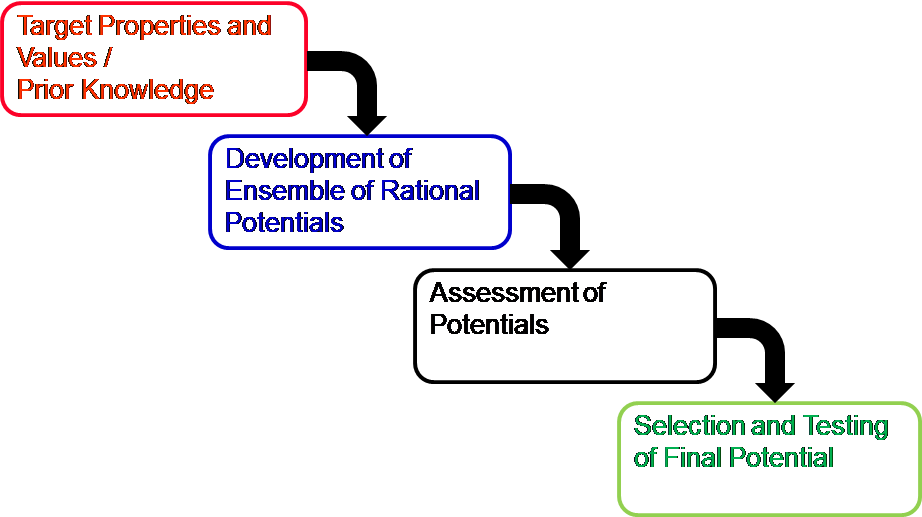
\includegraphics[width=0.8\textwidth]{chapter7/pareto_schematic}
  \caption{Schematic of the approach taken to potential development.}
  \label{fig:pareto_schematic}
\end{figure}

Figure \ref{fig:pareto_schematic} shows a schematic of the approach to the development of potentials outlined here. There are essentially four steps.
\begin{enumerate}
	\item The identification of structures, properties and their values to be used in the potential fitting. The specific values can be taken from experiment, from higher fidelity calculation methods such as quantum chemical or density functional theory (DFT) calculations, or a combination thereof. Our approach in this step is similar to standard potential development approaches.
 \item The use of ideas from Pareto optimization to develop an ensemble of rational potentials.  The concept of Pareto optimality was introduced discussed in Chapter \ref{ch:potential_development}. The term ‘rational’ will be discussed in detail below, but involves the use of a simple algorithm to identify potential parameterizations that make sense to consider further. This is the central idea of our approach and is very different from a conventional potential fitting approach
 	\item The analysis of the ensemble of rational potentials to identify features and clustering in both the high-dimensional parameter space and in the high-dimensional space of errors in the predictions of the properties.
 	\item The down-selection and testing of a few parameterizations or a single parameterization of the potential for use in further simulations.
\end{enumerate}

We focus mainly on the second of these steps: the development of an ensemble of rational potentials. We do, however, briefly discuss the other three parts of the process. For concreteness, we illustrate their use in the development of potentials for MgO, a simple and archetype ionic material.

As an illustration of the kind of information which can be obtained using a Pareto approach to parameterization and an example of the procedure shown in Fig. \ref{fig:pareto_schematic}, we consider the case of Buckingham potentials for magnesium oxide (MgO).

\section{Potential Formalism and Prior Knowledge}

Lewis and Catlow\cite{lewis1985_buckingham} parameterized a wide range of oxide systems with a pairwise potential, between two atoms $i$ and $j$.  In this formalism, the physics of an ionic system can be modelled with a pairwise Coulombic interaction between atoms $i$ and $j$, a short range repulsion due to the Pauli exclusion principle, and a van der Waals interaction term\cite{buckingham1938}

\begin{equation}
	V_{\alpha\beta}(r_{ij}) =
			\frac{Z_{\alpha}Z_{\beta}e^2}{r_{ij}}
			+ A_{\alpha\beta} \exp \left(\frac{r_{ij}}
																				{\rho_{\alpha\beta}}
															\right)
			- \frac{C_{\alpha\beta}}
			       {r_{ij}^6},
\end{equation}
with $\alpha$ and $\beta$ representing the chemical species of atoms $i$ and $j$, respectively.  The free parameters of the potential are $A_{\alpha\beta}$, $\rho_{\alpha\beta}$, and $C_{\alpha\beta}$ and $Z_i$.  The ionic charges which are allowed to deviate from their from their formal charges.  This information will be encoded as constraints to our optimization problem.

We examine three existing Buckingham potentials for MgO to define our initial vague (uninformed) estimate of the $p{\bm{\theta}}$ by assuming a uniform distribution on the domain of possible values of $p{\theta_i}$ defined by a lower and upper bound for each parameter $i$. Since MgO must be charge neutral, we restrict $Z_{\text{Mg}}= -Z_{\text{O}}$. For simplicity, and as is typical for Buckingham potentials, the Mg-Mg short-range interactions are set to zero ($A_\text{Mg-Mg}=0$ with $\rho_{\text{Mg-Mg}}=0.5$  for numerical stability), as is the van der Waals term for the Mg-O interaction ($C_{\text{Mg-O}}=0$). This leaves six free parameters in which to fit the potential (
$A_{\text{O-O}}$,
$\rho_{\text{O-O}}$,
$C_{\text{O-O}}$,
$A_{\text{Mg-O}}$,
$\rho_{\text{Mg-O}}$, and
$Z_{\text{Mg}}$).

In addition to the potential from Lewis and Catlow, two potentials unpublished Buckingham potentials were developed by Ball and Grimes (BG-2.0 and BG-1.7), but are available in the work of Henkelman \emph{et al.}\cite{henkelman2005_buckingham_MgO}.  For each parameter, we define the upper and lower bounds of the uninformative prior distribution from the three potentials in Table \ref{tlb:MgO_prior_potentials}, slightly increasing the range of values, as shown in Table \ref{tbl:MgO_inital_distribution}.

\begin{table}[ht]
	\caption{The Parameters for the empirical Buckingham potential for two formal charge potentials by Lewis and Catlow (LC)\cite{lewis1985_buckingham} and Ball and Grimes (BG-2.0). Another potential developed by Ball and Grimes (BG-1.7) uses partial charges. Parameters taken from Henkelman \emph{et al.}\cite{henkelman2005_buckingham_MgO}.}
	\label{tlb:MgO_prior_potentials}
	\centering
	\begin{tabular}{cccccc}
		\hline
		{Potential Name} & {$Z_{\text{Mg}}$ (e)} & Pair	 & $A$ (eV) & $\rho$ (\AA)	& $C$ ($\text{eV \AA}^6$) \\
		\hline
		LC	&    +2.00   &  Mg-O   &	 821.60  &   0.32000  &  0.00 \\
			  &            &   O-O	 & 22764.00	 &   0.14900  & 27.88 \\
		BG-2.0 & +2.00   &	Mg-O	 &  1279.69  &   0.29969  &  0.00 \\
		       &         & 	 O-O	 &  9547.96	 &   0.21916	& 32.00 \\
		BG-1.7 &  +1.70  &  Mg-O   &   929.69  &   0.29909  &	 0.00 \\
           &         &   O-O   &  4870.00	 &   0.26700  &	77.00 \\
		\hline
	\end{tabular}
\end{table}

\begin{table}[ht]
	\caption{Minimum and maximum values on the vague prior distribution for three parameters of the MgO Buckingham potential.}
	\label{tbl:MgO_inital_distribution}
	\centering
	\begin{tabular}{cccc}
    \hline
		$\theta_i$ & $\theta_i^{\text{MIN}}$ & $\theta_i^{\text{MAX}}$ & Units \\
		\hline
		$Z_{\text{Mg}}$ & +1.5 & +2.5 & e \\
		$A_{\text{Mg-O}}$ & +800.0 & +1300.0 & eV \\
		$rho_{\text{Mg-O}}$ & +0.2900 & +0.3300 & \AA \\
		$A_{\text{O-O}}$ & +500.0 & +2500.0 & eV \\
		$\rho_{\text{O-O}}$ & +0.1000 & +0.4000 & \AA \\
		$C_{\text{O-O}}$ & +25.00 & +75.00 & $\text{eV \AA}^6$ \\
	  \hline
	\end{tabular}
\end{table}

\subsection{Fitting Database}

We choose the target materials properties for MgO to be the lattice parameter, $a_0$, and elastic properties ($c_{11}$, $c_{12}$, $c_{44}$, and shear and bulk, $B$ and $G$) of the ground-state rock-salt (NaCl) structure, the \hkl(100) surface energy, the anion and cation Frenkel defect energies, and the Schottky defect formation energy.  Although $B$ and $G$ are fully determined by other elastic constants, it is useful to include them in the set of fitting database as they are the most physically accessible and measure the specific sums and differences in elastic properties that correspond to criteria for the stability of the crystal ($B > 0$, $G > 0$, $c_{44}> 0$).

Reference values for all of the targeted properties were calculated with VASP\cite{kresse1993_vasp,kresse1996_vasp1,kresse1996_vasp2} using the Perdew, Burke, and Ernzerhof generalized-gradient approximation (PBE-GGA) of the exchange-correlation functional \cite{perdew1996_gga_pbe}.
The lattice parameter and elastic properties were calculated from an 8-ion conventional cubic unit cell using a $6 \times 6 \times 6$ $k$-point mesh.  Surface energies were calculated using a $1 \times 1 \times 10$ supercell, with a slab thickness consisting of half of the height of the cell, and a $k$-point mesh of $9 \times 9 \times 1$.  Defect formation energies were calculated from $3 \times 3 \times 3$ supercells, using a $k$-point mesh of $3 \times 3 \times 3$.  The plane wave cutoff energy was set at $800$ eV. The resulting values of these quantities are showin in Table \ref{tbl:MgO_target} and constitute the QOIs for the parametrization process.

\begin{table}[ht]
	\caption[Target Properties of MgO]{Target properties of MgO and their values determined from DFT}
	\label{tbl:MgO_target}
	\centering
	\begin{tabular}{cccc}
		\hline
		 $q_i$ & Name & Units & {DFT (PBE-GGA)} \\
		\hline
    $q_1$ & $a_0$     & \AA   &	4.246 \\
    $q_2$ & $c_{11}$  & GPa   & 277.00 \\
    $q_3$ & $c_{12}$  & GPa   & 91.67 \\
    $q_4$ & $c_{44}$  & GPa 	& 144.01 \\
		$q_5$ & $B$       & GPa   & 153.45 \\
    $q_6$ & $G$       & GPa   & 92.66 \\
		$q_7$ & $E_{\text{fr,a}}$ & eV & 	10.978 \\
		$q_8$ & $E_{\text{fr,c}}$ & eV & 8.966 \\
		$q_9$ & $E_{\text{sch}}$ & eV &	5.067 \\
		$q_{10}$ & $\gamma_{\text{\hkl<100>}}$ & $\text{eV/\AA}^2$ &	0.056 \\
		\hline
	\end{tabular}
\end{table}

\section{Development of Ensemble of Rational Potentials}

With the identification of constraints and a fitting database determined, it is possible to define the parameterization problem.  Here, after choosing the loss function between predicted values $\hat{q}_i(\bm{\theta})$ and the target value $q_i$ with the absolute value function, $L_i(\bm{\theta})=|\hat{q}_i(\bm{\theta})-q_i|$ for each QOi $q$.q
\begin{align}
	&\min_{\bm{\theta}} &\bm{L}(\bm{\theta})=[
	    L_1(\bm{\theta}),
			L_2(\bm{\theta}),
			...,
			L_9(\bm{\theta})] \\
	&\text{subject to} &g_1: Z_{\text{Mg}} > 0.0 \\
	& &g_2: A_{\text{Mg-O}} > 0.0 \\
	& &g_3: \rho_{\text{Mg-O}} > 0.0 \\
	& &g_4: A_{\text{O-O}} > 0.0 \\
	& &g_5: \rho_{\text{O-O}} > 0.0 \\
	& &g_6: C_{\text{O-O}} < 0.0 \\
	& &g_7: B > 0 \\
	& &g_8: G > 0 \\
	& &g_9: c_{44} > 0 \\
  & &h_1: Z_{\text{O}} = -Z_{\text{Mg}} \\
  & &h_2: A_{\text{Mg-Mg}} = 0.0 \\
  & &h_3: \rho_{\text{Mg-Mg}} = 0.5 \\
	& &h_5: C_{\text{Mg-O}} = 0.0 \\
  & &h_4: C_{\text{Mg-Mg}} = 0.0
\end{align}
where $g_i$ are inequality constraints and $h_i$ are equality constraints.

The machine-learning process of the generation of parameter sets, simulation management, and parallelization are provided through software developed in Python and MPI, as discussed in Chapter \ref{ch:software}. The energy calculations are performed using the LAMMPS\cite{plimpton1995_lammps} code. Long-range Coulombic interactions are computed in LAMMPS using the particle-particle mesh\cite{hockney1988_ppm}.  The entire autonomous workflow was illustrated in Figure \ref{fig:pareto_optimization}. The random generation of parameters sometimes results in an unusable potential (e.g. a failure in structural minimization); these parameters (less than 10\% of those tried) are discarded and are not included among the final 10,000 parameterizations.
Sampling from the vague distributions defined above, we generate N=10,000 sample potential parameterizations. The Pareto points are identified by removing the dominated points; This results in a Pareto set of  $N_\text{pareto} = 955$ potentials that provide a first estimate of the six-dimensional Pareto surface. We use the distribution of parameters in this Pareto set to provide a better estimate of the distribution functions of the parameters.  While an empirical discrete non-parametric probability distribution function can be calculated from the histogram of parameters of the Pareto optimal potentials, it is preferable to sample a random variable defined by a smooth, and continuous probability distribution function. The kernel density estimation (KDE) provides a parameter-free estimate of the probability density functions\cite{rosenblatt1956_kde,parzen1962_kde} and provides the ability to uncover features in the estimate of probability density function which are not apparent in the histogram. If we assume each member of the Pareto set to be independent and identically distributed from some distribution with unknown density $p_{\Theta^*}$, we can the estimate of the shape of $p(\bm{\theta}^*)$, which we now define exactly.
Let $\bm{\theta}_{t-1,1}^*,...,\bm{\theta}_{t-1,N}^*$ be $N$ samples of $N_P$-dimensional parameter sets belonging to the Pareto set from the previous iteration, $t-1$, be described by the density function $\hat{p}_{\bm{\Theta}}(\bm{\theta}_t)$.  The multivariate kernel density estimate is defined to be
\begin{equation}
	\hat{f}_{\bm{\Theta}_t}(\bm{\theta}|\bm{H})
			= \frac{1}{N}\sum_{i=1}{N}\bm{K}_{\bm{H}}(\bm{\theta}-\bm{\theta}_i)
\end{equation}
where $\bm{K}_{\bm{H}} = |\bm{H}|^{-1/2} K ({\bm{H}}^{-1/2}\bm{\theta})$ with $K$ being a kernel function which is has a symmetric multivariate density, $\bm{H}\in \mathbb{R}^{N_P\times N_P}$ is bandwidth matrix which is symmetric and postive definite.  Since the choice of the kernel function is not critical to the accuracy of kernel density estimators in most cases\cite{wand1995_kde}, the Gaussian kernel is chosen.  Then $\bm{H}$ is the bandwidth matrix which affects the direction and orientation of smoothing induced.
Here, $\bm{H}$ is determined from the covariance matrix for the parameter matrix from the previous iteration is used $\bm{\Theta}_{t-1}$, and modified by a scaling factor determined by the Silverman method\cite{silverman1986_kde}, which minimizes the mean integrated square differences.

Figure \ref{fig:Z_Mg_iter_0} illustrates the distribution of the ionic charge of Mg ions, $Z_{\text{Mg}}$, after sampling from the uniform distribution.  Since $Z_{\text{Mg}}$ is initially sampled from a uniform distribution, the histogram indicates the strict discontinuous limits of the lower and upper bounds of the distribution.  The coarse-grained nature of the discrete bins in the histogram would make it difficult to identify the most probable values of $Z_{\text{Mg}}$ or even the departure of the Pareto set population from the original uniform distribution from which $Z_{Mg}$ is generated.  Attempting to use the normal distribution from the sample mean and variance does not capture the underlying features of the uniform.  However, the KDE is able to estimate the underlying probability distribution function with some distortion at the upper and lower bounds due to exponential tails of the Gaussian distribution.

\begin{figure}[ht]
	\centering
  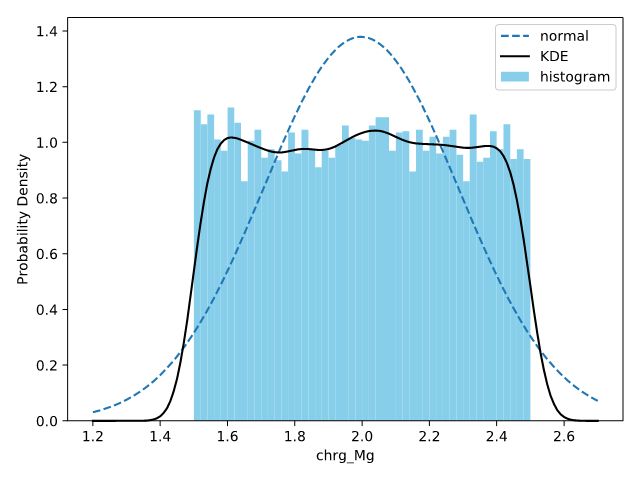
\includegraphics[width=0.8\textwidth]{chapter7/Z_Mg_iter_0}
  \caption{The distribution of the parameter which controls the partial charge distribution of the magnesium ion, $Z_{\text{Mg}}$, in the Pareto set. The histogram of which is a discrete representation of the distribution of $Z_{\text{Mg}}$, continuous distributions of the distribution of $Z_{\text{Mg}}$ is estimated by the kernel density estimate.}
  \label{fig:Z_Mg_iter_0}
\end{figure}

Figure \ref{fig:Z_Mg_iter_0_pareto} illustrates the changes in the KDE as it goes through sampling, Pareto-optimality filtering, and performance filtering.  The blue dashed line shows the distribution in charge for all points sampled. When the dominated parameterizations are removed from the set to determine the Pareto set, the KDE (orange dashed line) indicates a concentration of parameterizations in the region $Z_{\text{Mg}} \approx +1.8 \text{e}$.  Next, we cull the Pareto set by removing the largest outliers by percentile, determined by $|\hat{q}_i -q_i|$.  This eliminates $2$\% of pathological parameterizations which are Pareto efficient; this results in the green dashed line in Figure \ref{fig:Z_Mg_iter_0_pareto}.

\begin{figure}[ht]
	\centering
  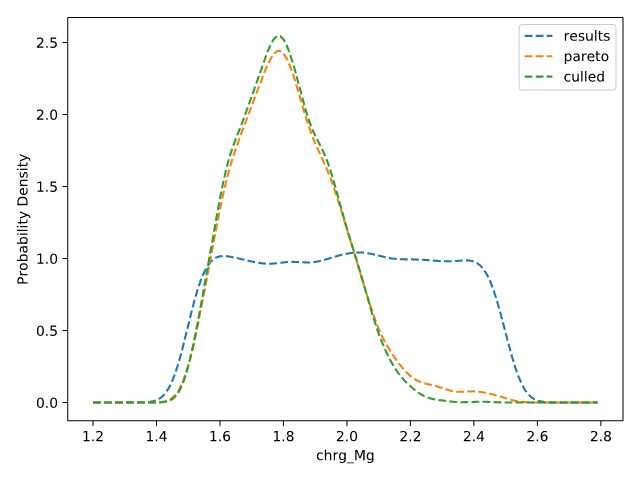
\includegraphics[width=0.8\textwidth]{chapter7/Z_Mg_iter_0_pareto}
  \caption{A single variable visualization of the population of parameterization for the charge parameter, $Z_{\text{Mg}}$ after the first iteration}
  \label{fig:Z_Mg_iter_0_pareto}
\end{figure}

Ten iterative improvements are made to estimate the Pareto surface using updates to the KDE probability distribution described earlier using the Silverman selection of the smoothing parameter. The evolution of the set of solutions comes from the refinement of the probability density function which represents the set of solutions.  In the initial iteration (N=0), the probabiity distribution resembles a uniform distribution.  The probability distribution evolves rapidly to a triangular shaped probability distribution made smooth by the KDE Gaussian tails, but the resolution of the region of maximum likelihood (the peak of the density function does not happen until $N=9$

\begin{figure}[ht]
	\centering
  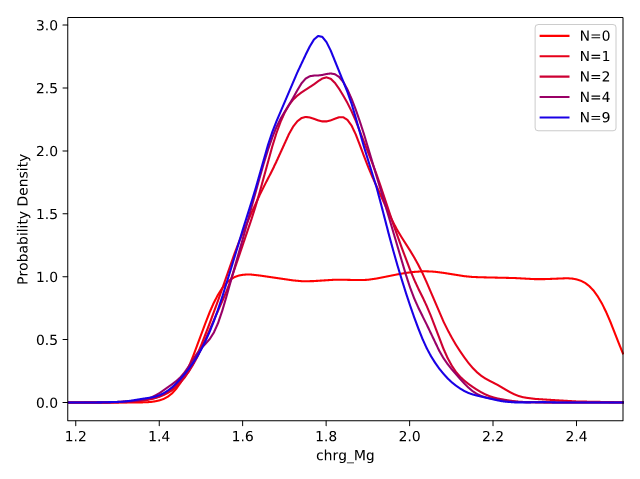
\includegraphics[width=0.8\textwidth]{chapter7/Z_Mg_evolution}
  \caption{Evolution of the predicted charge parameter $Z_{\text{Mg}}$.  These curves are the univariate probability distribution function, using the Silverman method for determining the smoothing parameter.}
  \label{fig:Z_Mg_evolution}
\end{figure}

Since the number of materials properties constitutes a high-dimensional space, analysis of the Pareto surface is most conveniently performed in a series of bi-objective scatter plots which project, or slice, the error-space information onto the the 2D space.  A representative improvement of the Pareto surface estimate is shown in Figure \ref{fig:MgO_biobjective_evolution}, which shows the first four iterations of Pareto estimation process by looking at,
$|\epsilon_i(\bm{\theta})=|\hat{q}_i(\bm{\theta})-q_i|$, $\bm{\theta}\in\bm{\Theta}_t^*$ for the bulk modulus ($B$) and the lattice parameter ($a_0$).  This bivariate plot projects the $N_Q$ dimensional $\epsilon$-space is projected onto tje two-dimensional $\epsilon$-space for $B$ and $a_0$. In the initial iteration, the uniformative distribution selects a range of parameter which have large errors.  In subsequent iterations, the KDE predicts parameterizations in the neighborhood of previously found Pareto optimal points resulting in $q(\bm{\theta})$ being clustered closer to the origin.   The KDE is explictly chosen because for the ability to capture departures from the multivariate-normal distribution.  There are points close to the origin in this-two dimesional project of the Pareto surface; however, these points do not have small errors in the other properties.

\begin{figure}[ht]
	\centering
  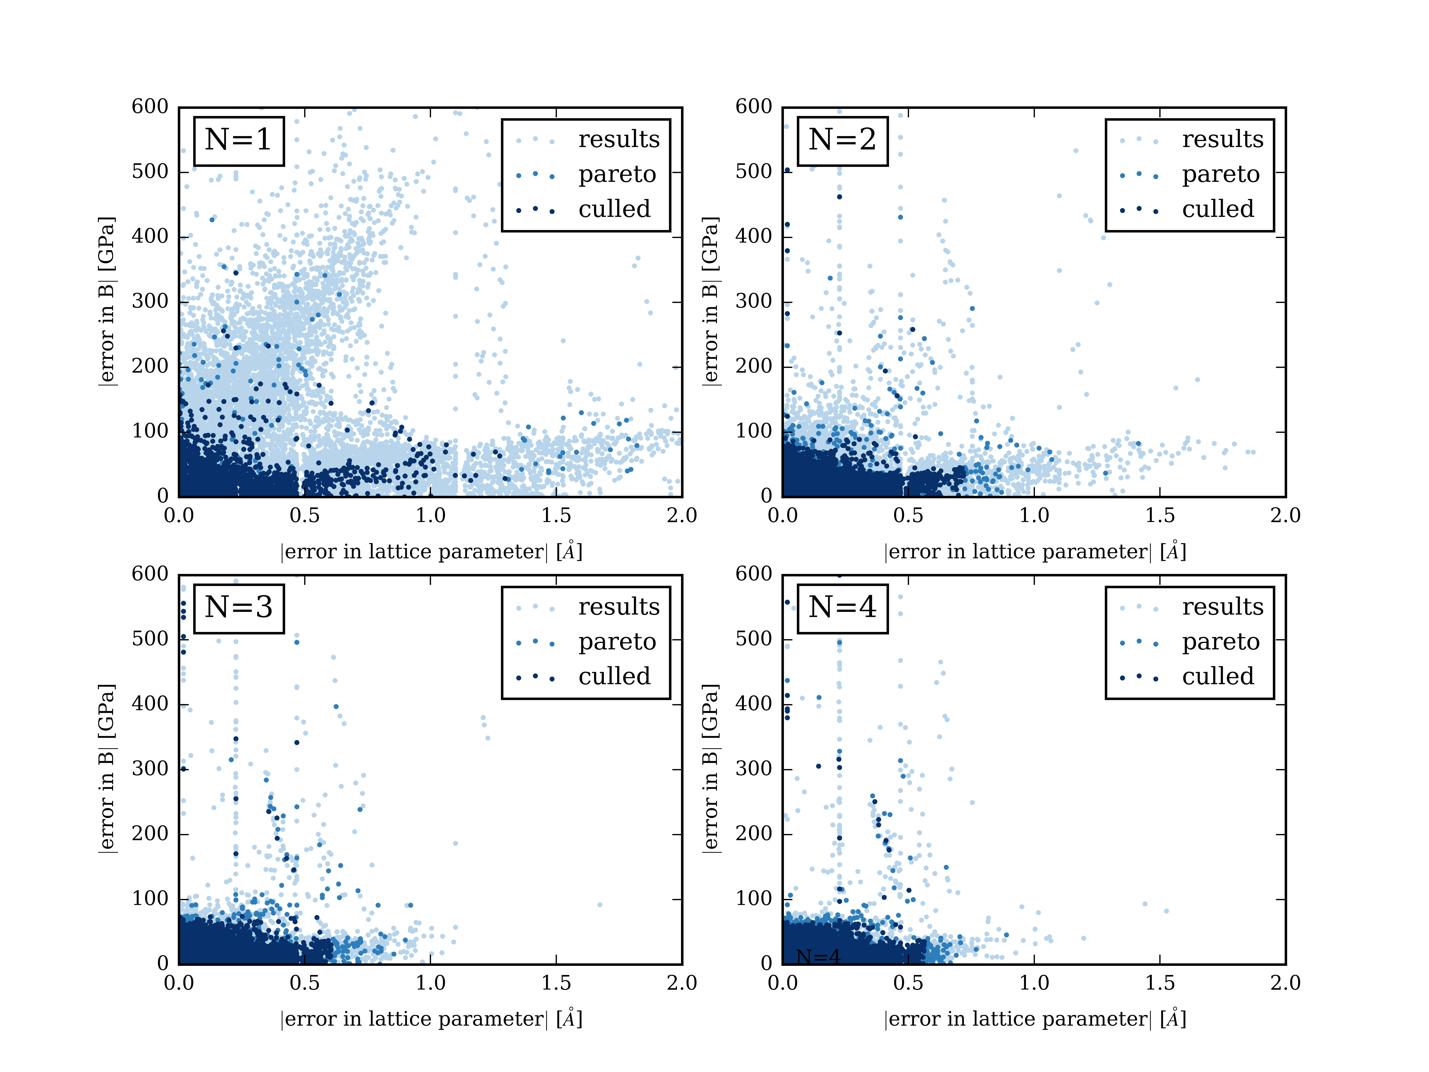
\includegraphics[width=0.8\textwidth]{chapter7/MgO_biobjective_evolution}
  \caption{Evolution of the predicted charge parameter $Z_{\text{Mg}}$.  These curves are the univariate probability distribution function, using the Silverman method for determining the smoothing parameter.}
  \label{fig:MgO_biobjective_evolution}
\end{figure}

In a multivariate-normal distribution, the correlation between parameters may be significant, and is captured in the variance-covariance matrix. This allows for more sophisticated analysis and refinement of the distribution functions. For example, the relationship between the parameters $A_{\text{O-O}}$ and $\rho_{\text{O-O}}$ are captured in Figure \ref{fig:MgO_biobjective_A_v_rho_OO}.  A visual inspection of the data shows a negative correlations between the two terms; as $A_{\text{O-O}}$ increases  $\rho_{\text{O-O}}$ tends to decrease.  This relationship is not surprising since these two quantities both parameterize the exponential repulsion, for which an increase in the decay length, $\rho$, can be compensated for by a decrese in the prefactor, $A$, and vice versa.

\begin{figure}[ht]
	\centering
  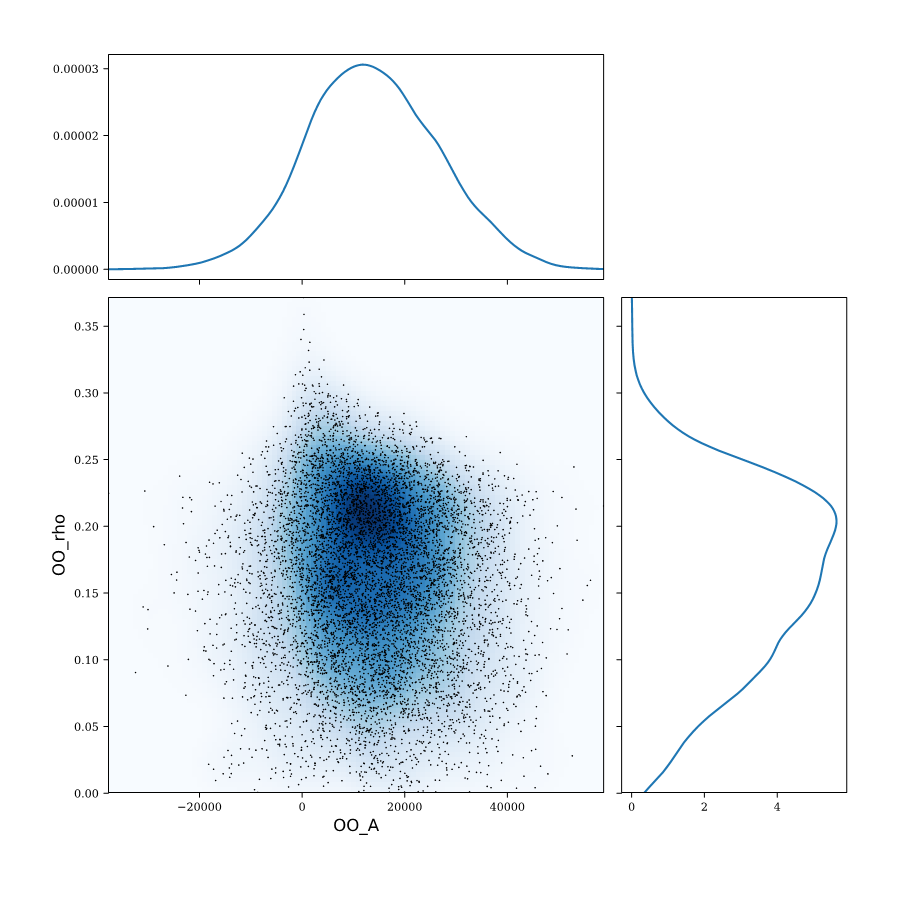
\includegraphics[width=0.8\textwidth]{chapter7/MgO_biobjective_A_v_rho_OO}
  \caption{Probability density functions and joint probability density functions of the KDE representing set of solutions for parameters $A_{\text{O-O}}$ and $\rho_{\text{O-O}}$.  The main figure is the joint probability density function with darker values being higher probability regions.  The vertical and horizontal probability density functions.}
  \label{fig:MgO_biobjective_A_v_rho_OO}
\end{figure}

When this iterative process is complete, we have an ensemble of $N=7557$ Pareto efficient MgO Buckingham potentials and associated potential parameters.

To this point in the process, unlike the gradient method, the potential developer has not provided any information as to their preferences in terms of acceptable errors or weights. Rather, the process has been an objective analysis of the capablities of the potential form to reproduce the targeted materials properties.  Thus, this process is complectely algorithmic in that for the potential form and target values, another developer should produce a statisitcially identical ensemble of Pareto optimial potentials. Further, if the the vague prior, iteration sequence and random numbers used in the sampling are defined, another developer should reproduce exactly the same ensemble of potentials.

An iterative procss can continue indefintiely. Thus, we need to establish criterea for satisfactory convergence. In deterministic methods, the numerical refinement is halted by a convergence condition, where the numerical solution changes slow as the optimal solution is approached.  The solutions to a multi-objective problem are a set of solutions.  Our solution method represents the set of solutions as a probability density function, which are estimated from the \emph{Pareto set}, the parameterizations which produce the Pareto surface in objective space, $\bm{\Theta}_i^*$, for the $i$th iteration.  A statistical analog to numerical convergence is to assess the convergence of the distribution, where we look at the difference of the distribution of the samples as a measure of convergence. The Kullback-Liebler\cite{kullback1951_kld} divergence, $D_{\text{KL}}(f_1 \vert f_2)$, measures how one probability distribution, $f_1$, diverges from a second probability distribution function, $f_2$.  For continuous random variables, $D_{\text{KL}}$, is defined as the integral
\begin{equation}\label{eq:kld}
    D_{\text{KL}} - \int f_1(x) \log \frac{f_1(x)}{f_2(x)} dx
\end{equation}
$D_{\text{KL}} \geq 0$, with $D_{\text{KL}} (f_1 \vert f_2 )=0$, when $f_1$=$f_2$, almost everywhere.  For our application, our distributions are KDEs, so the evaluation of the integral can be done by Monte Carlo integration\cite{hershey_kld_mc_integration}.  As the number of iterations, $i$, increases, the Kullbach-Liebler divergence $D_{\text{KL}}(f_{i-1}\vert f_i )$, converges asymtotically to $0$.

Since early iterations are more likely to cause changes in the set approximating $\bm{\Theta}^*$ than later simulations, changes in $D_{\text{KL}}$ will initially be large.  However, it becomes increasingly more difficult to identify further Pareto optimal solutions later in the simulation.  As a result, the distribution becomes more stationary.  However, since this integral is evaluated by Monte Carlo estimation, the KDE estimate of the distributions from the sample population will have small divergences betweem, $f_i(\bm{\theta}) and f_{i-1}(\bm{\theta})$, even if the KDE is the same distribution function.

Even 2D views of the Pareto set can identify shortcomings with potential formalisms.  The bi-objective plot in Figure \ref{fig:MgO_bivariate_c11_v_c44}, a slice through the data rather than projection of all of the data, illustrates a well-known limitation with the form of the Buckingham potential: there is a strong relationship between the $c_{11}$ and the $c_{44}$ of the elastic tensor, making reduction in the error of one lead to an increase in error in the other.

\begin{figure}[ht]
	\centering
  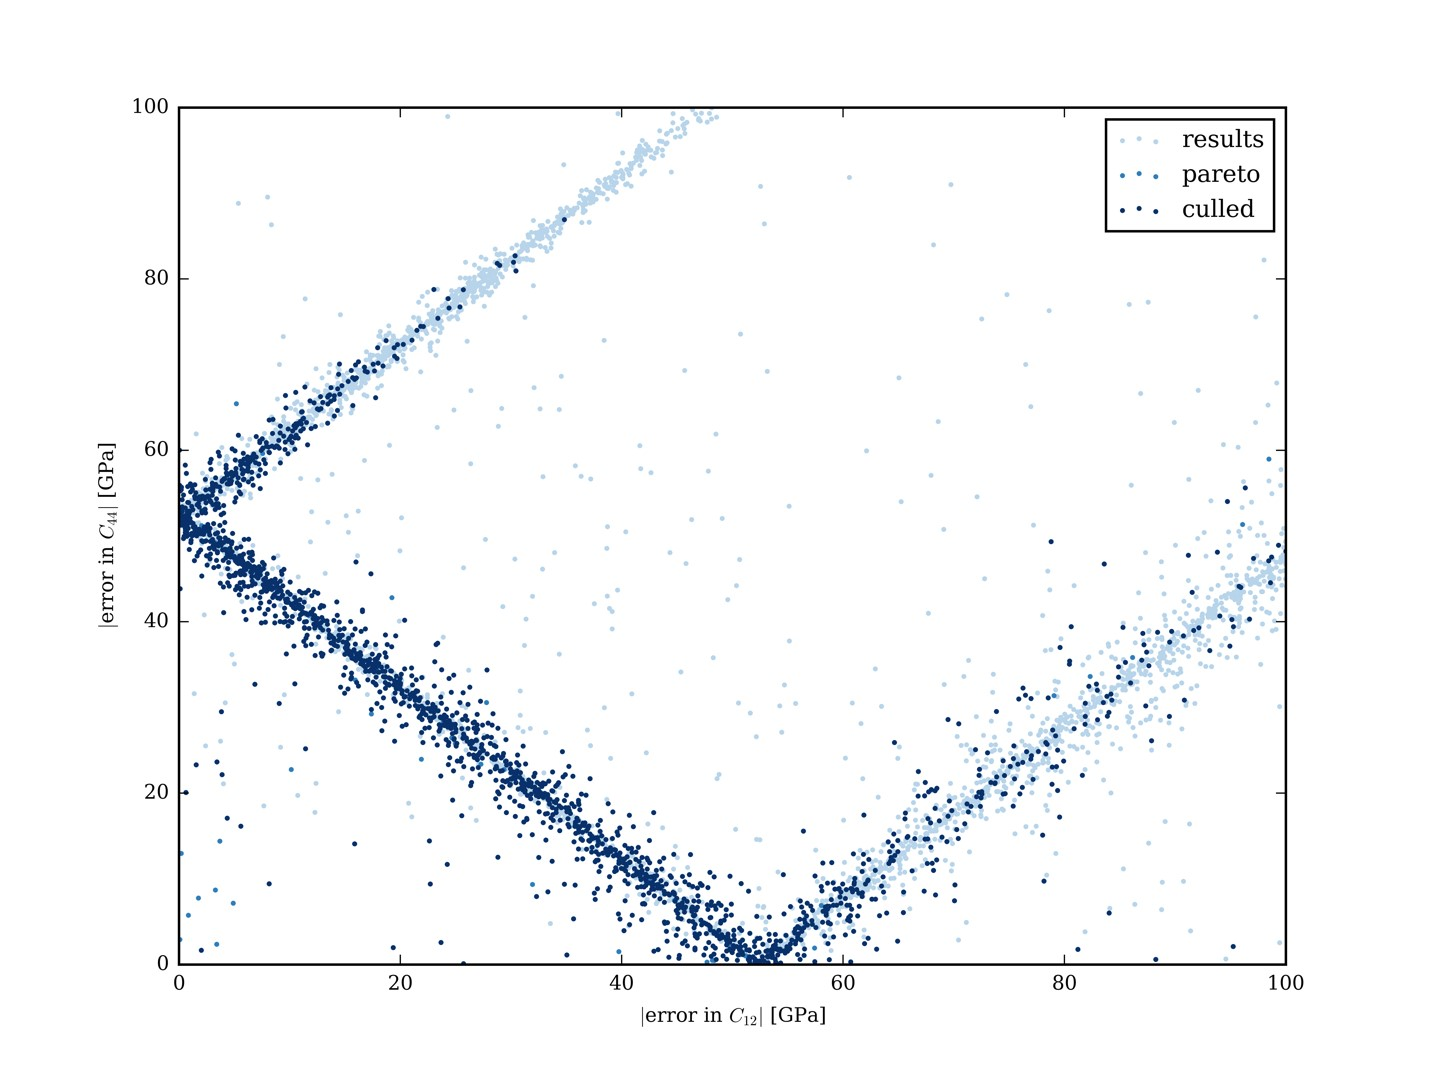
\includegraphics[width=0.8\textwidth]{chapter7/MgO_bivariate_c11_v_c44}
  \caption{Projection of the Pareto surface  in $\epsilon$-space projected onto the $|\epsilon_{c_{12}}|$ and $|\epsilon_{c_{44}}|$ subspace.  The 2D slice of data identifies a key tradeoff of the Buckingham potential.}
  \label{fig:MgO_bivariate_c11_v_c44}
\end{figure}


\section{Assessment of Potentials and Selection of Final Potentials}

Having generated an ensemble of Pareto-optimized potentials, the challenge now lies in down-selecting to a final set potentials for testing and full evaluation. The analysis performed to this point has been essentially algorithmic. For a specific formalism and specific material, the only input provided by the developer has been the properties to be considered in the fitting and their target values. Notably absent in the analysis to this point has been any statement of the acceptable errors in any of the targeted properties or any weighting factors. Rather, the analysis purely characterizes the capabilities of the potential. The result has been the Pareto optimal ensemble of interatomic potentials, any one of which is a rational choice in the sense of minimizing the errors. For an MD simulation, it is necessary to use a single potential; that is the developer must select one of the hundreds or thousands of rational choices coming from the Pareto analysis.  It thus at this stage of the process that the developer introduced their preferences into the analysis, thereby enabling the down-selection process.

	There are numerous ways of going about this process; unlike the construction of the Pareto ensemble, it is not uniquely defined.  As an illustration of one simple approach, we begin by normalizing the errors, $\epsilon_i$, by the target value, $q_i$; these normalized errors are now all dimensionless and are typically of order unity.  The 10 potentials closest to the origin, defined as the unweighted normalized sum of the squared scaled errors, are selected for further analysis.  In Figure \ref{fig:MgO_qoi_rugplots}, the performances of these $10$ Pareto-efficient potentials (black lines) are compared to potentials of Lewis-Catlow (green), Ball-Grimes±2.0 (blue), and Ball-Grimes±1.7 (red) potentials with respect to target values in Table \ref{tbl:MgO_target}. It is clear that the Pareto efficient potentials result in lower errors in the predicted values of almost all target physical quantities as compared to the expertly-determined reference potentials.

Having down-selected to 10 potentials, it is important to test their performances for properties that are not included in the fitting process. We calculate materials properties for quantities which are not part of the training set.  Specifically, we calculate the frequency of the zone-center optical phonon frequency for MgO, and the linear thermal expansion coefficient.  The phonon calculations are evaluated for the primitive cell of the rocksalt structure using GULP\cite{gale2003_gulp}.  The thermal expansion is determined from MD simulations. These results are compared from DFT-GGA calculations in the case of phonons ($385 \text{cm}^{-1})$, and from experimental data ($1.08\times10^{-5}$ \\A/\degree C) \cite{ho1998_thermal_expansion} in the case of thermal expansion.

\begin{figure}[ht]
	\centering
  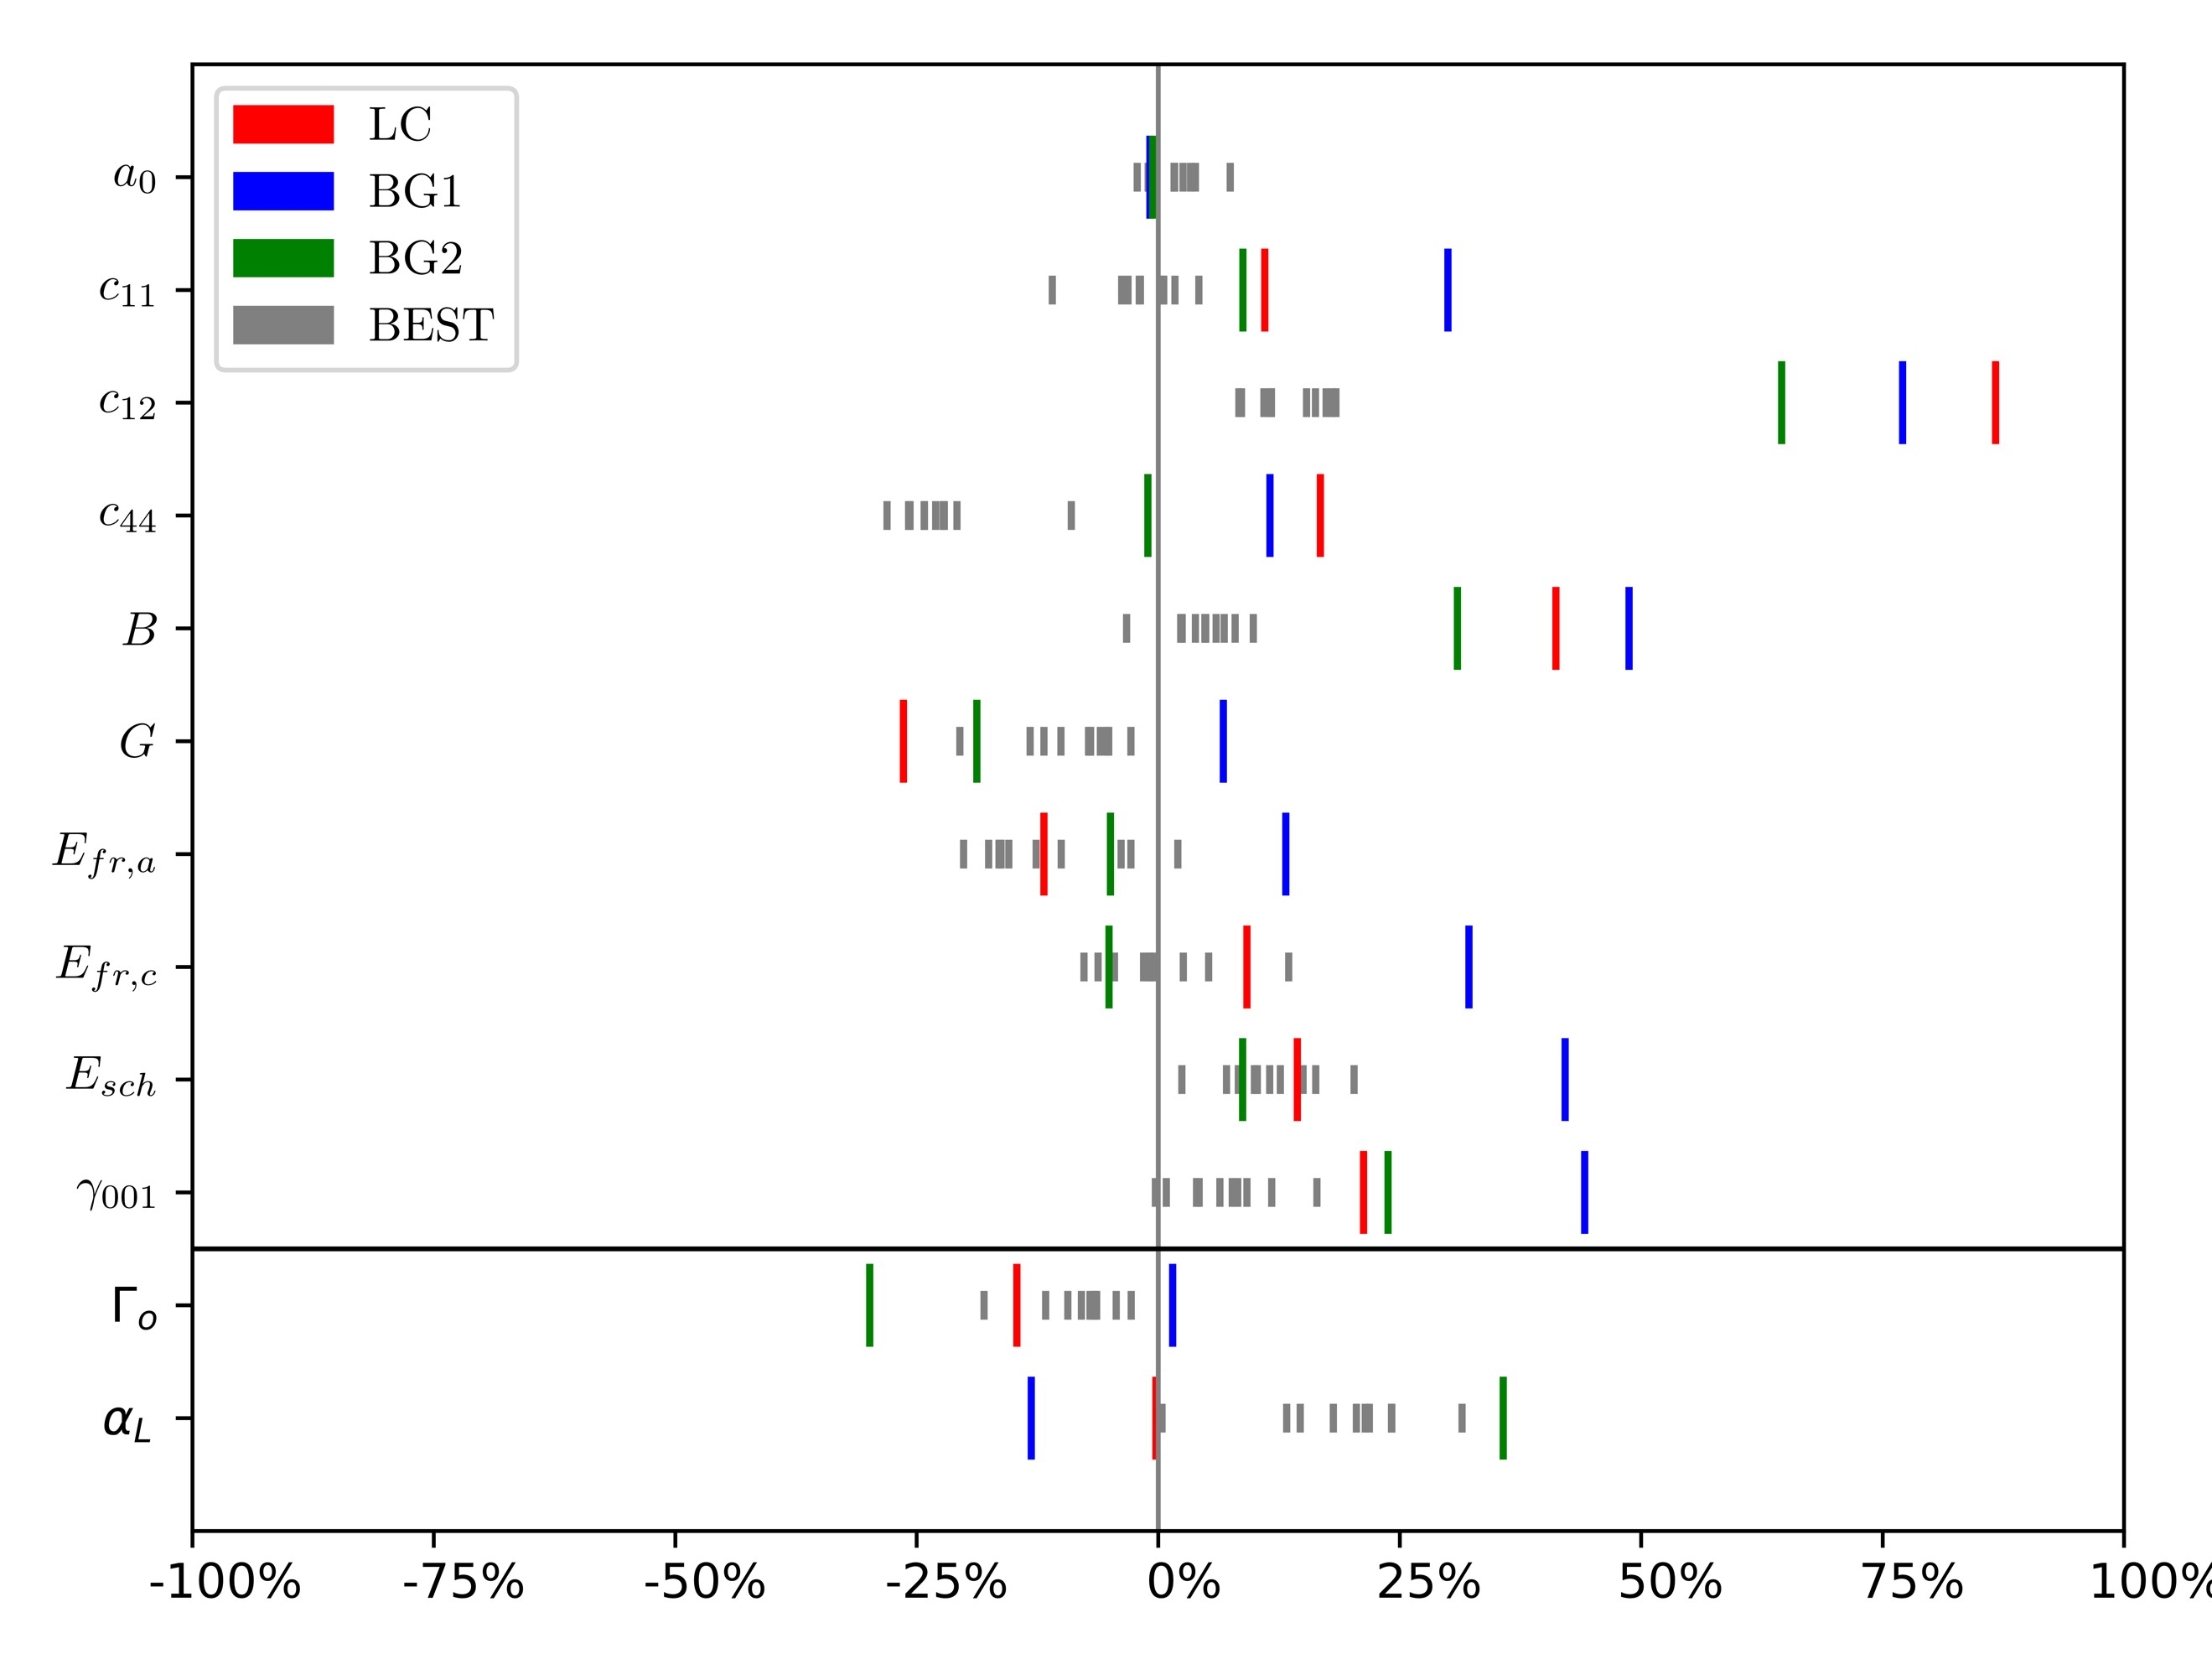
\includegraphics[width=0.8\textwidth]{chapter7/MgO_qoi_rugplots}
  \caption{Comparison of the errors in target quantities for 10 Pareto efficient parameterizations (black bars) of the Buckingham potential for MgO with predictions of three expert-developed potentials. The reference values are from the DFT calculations.}
  \label{fig:MgO_qoi_rugplots}
\end{figure}


To characterize this further, Figure \ref{fig:MgO_qoi_parallel_plots} compares the 10 best potentials selected in the way defined above to the LC, BG-2.0 and BG-1.7 potentials. Again, it is clear that in general, the potentials determined in this autonomous, machine-learning approach provide as high materials fidelity as the expert-developed potentials. The parameters and property values for these 10 best potentials and the three expert-developed potentials are shown in Tables \ref{tbl:MgO_best_param} and \ref{tbl:MgO_best_qoi}.

\begin{figure}[ht]
	\centering
  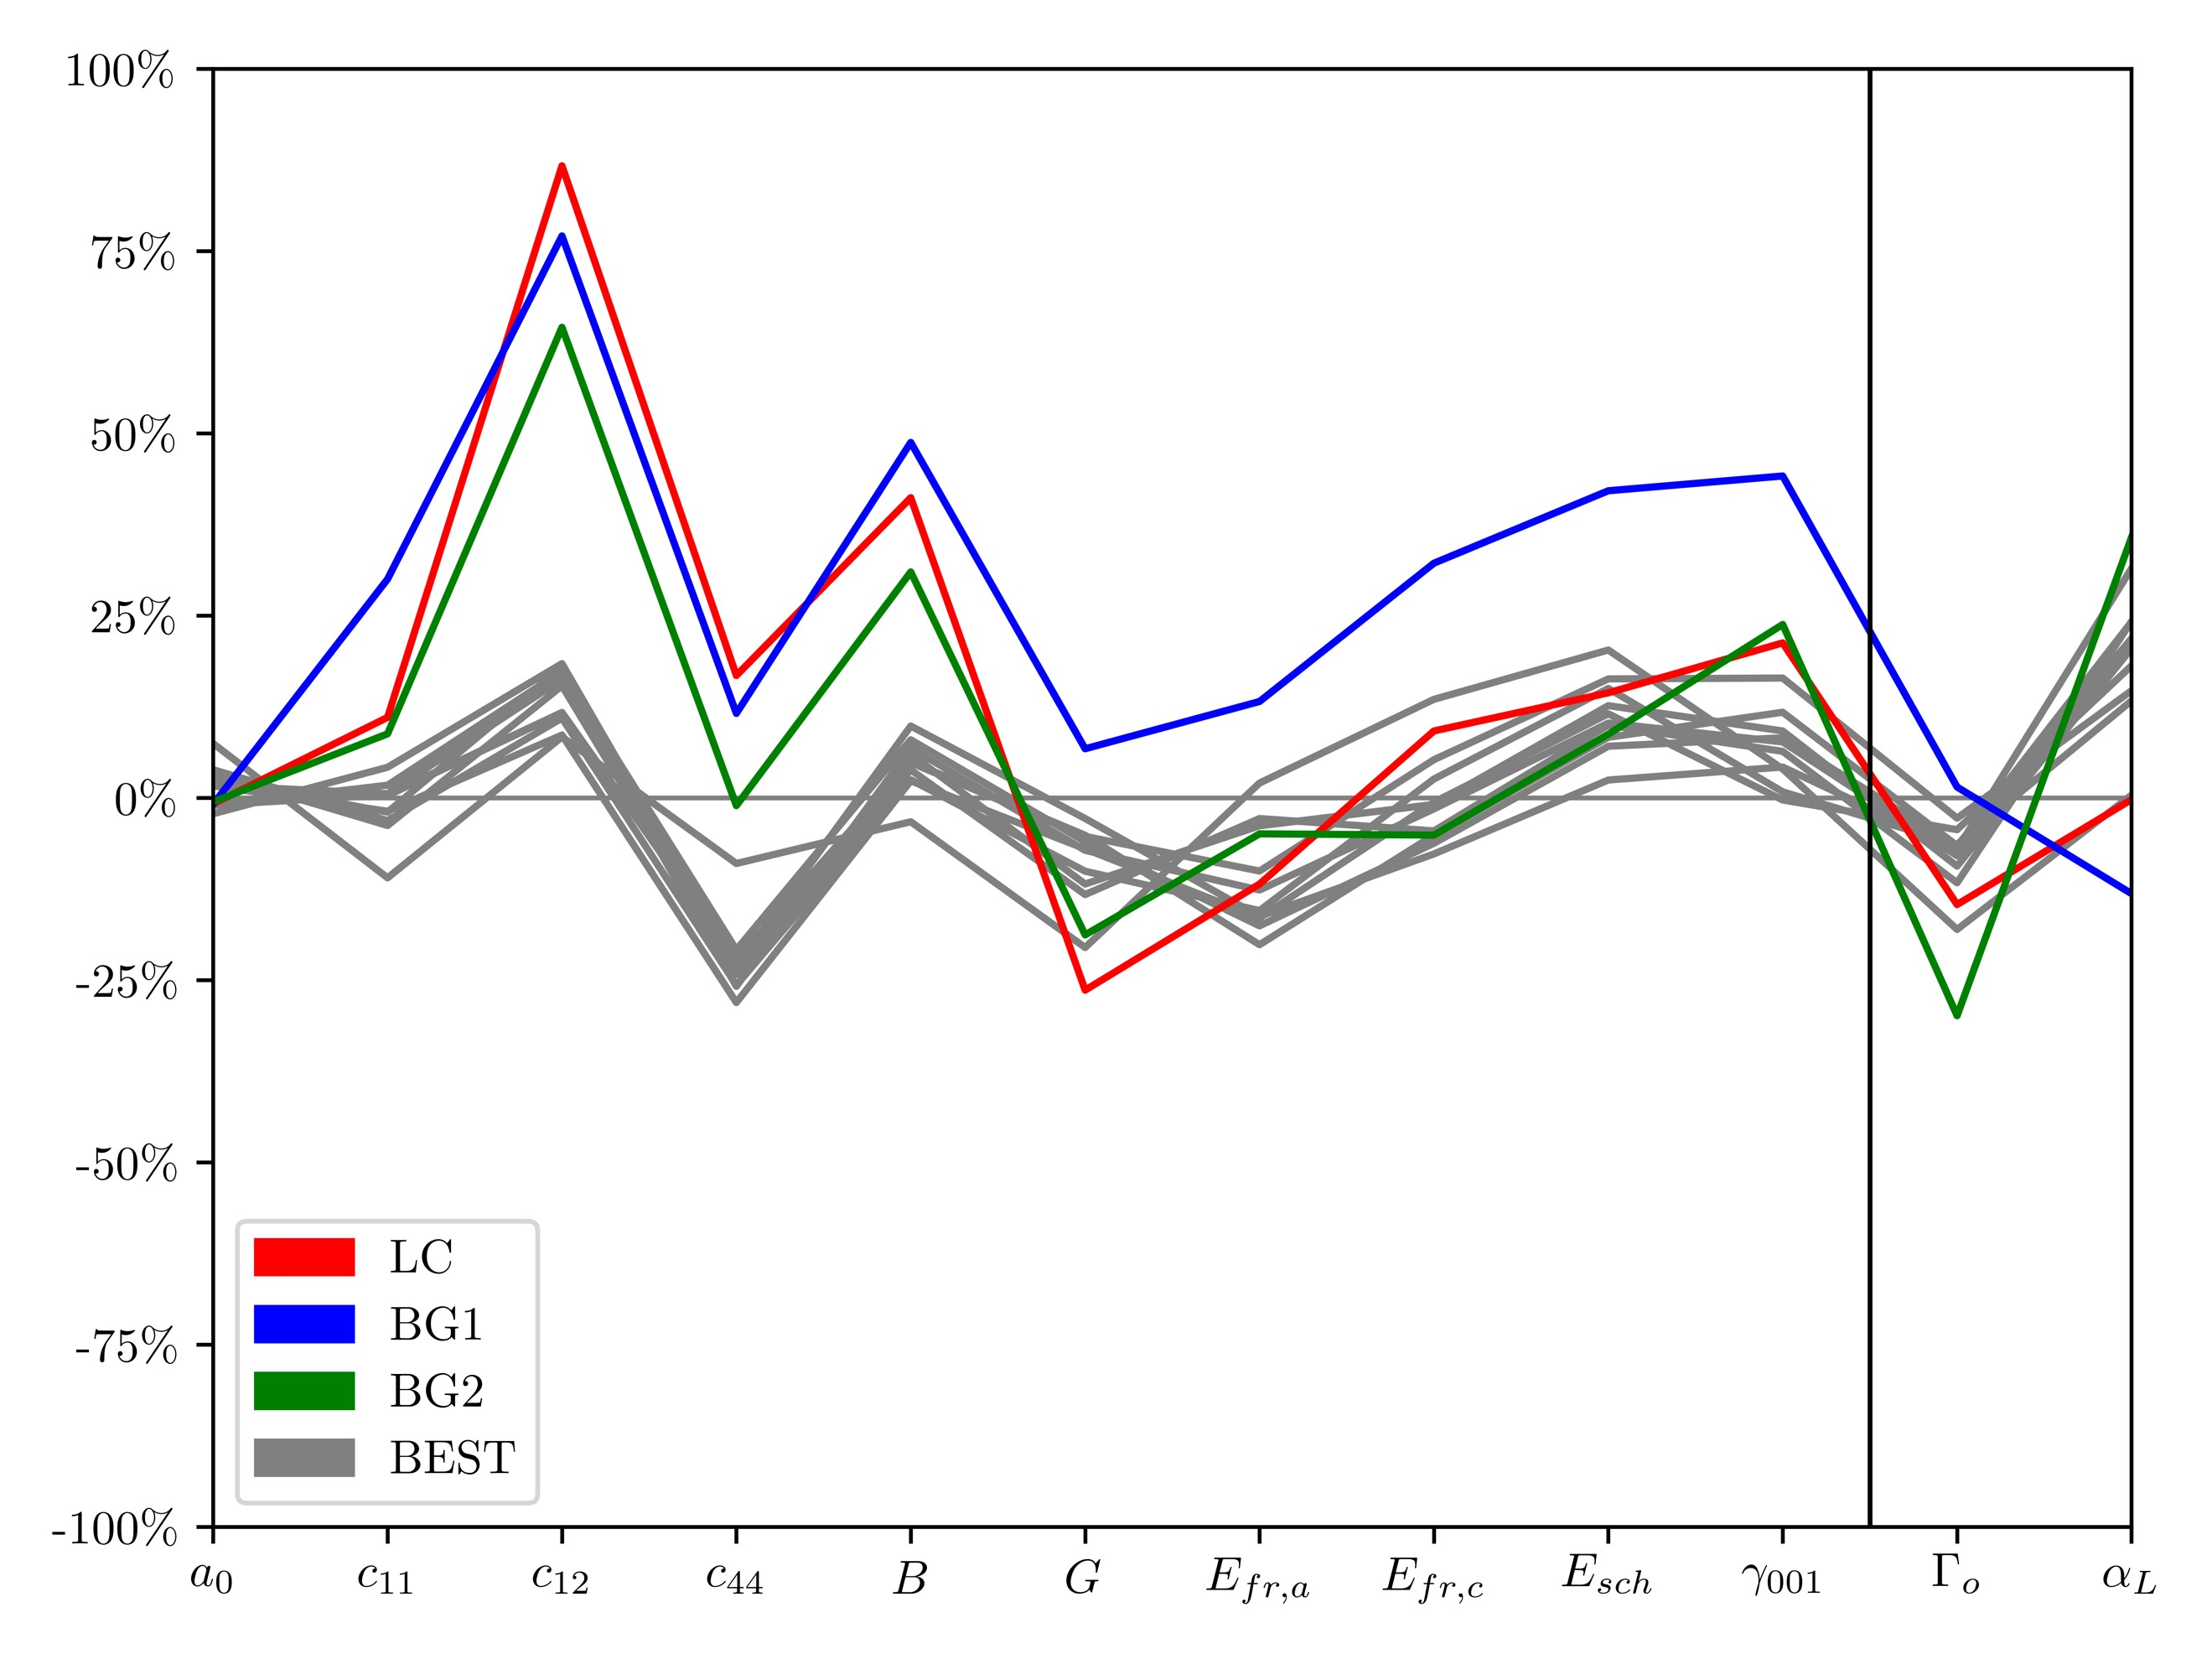
\includegraphics[width=0.8\textwidth]{chapter7/MgO_qoi_parallel_plots}
  \caption{Errors for the 10 best potentials and the LC and two BG potentials with the same labeling as in the previous figure. The overall best potential determined from our Pareto analysis is given the thick gray line. The QOIs to the left of the vertical line are used in the paramterization; those to the right are predictions.}
  \label{fig:MgO_qoi_parallel_plots}
\end{figure}

\begin{table}[ht]
	\caption{Parameters of the the three expert-develop potentials and the 10 potentials, out of 7557 Pareto optimal potentials with the normalized lowest squared errors.}
	\label{tbl:MgO_best_param}
	\centering
	\begin{tabular}{ccccccc}
		\hline
		{sim\_id} & $Z_{\text{Mg}}$ & $A_{\text{Mg-O}}$ & $\rho_{\text{Mg-O}}$ & $A_{\text{O-O}}$ & $\rho_{\text{O-O}}$ * $C_{\text{O-O}}$ \\
    \hline
		LC  & 2.0 & 821.60   & 0.32000 & 22764.00 & 0.14900 & 27.88 \\
		BG1 &	2.0 &	1279.69  &	0.29969 &	9547.96 &	0.21916 &	32.00 \\
		BG2 &	1.7	& 929.69   & 0.29909 & 4870.00 & 0.26700 & 7.00 \\
		550 &	1.6	& 1270.77	 & 0.28993 &	25294.69 & 0.23093 & 64.71 \\
		762  &	1.6	& 1093.66	 & 0.28812 &	27681.46 & 0.19519 & 33.99 \\
		5965 &	1.6	& 1011.10	 & 0.29378 &	15450.62 & 0.20124 & 44.60 \\
		8984 &	1.7	& 1410.19	 & 0.28510 &	27180.53 & 0.06775 & 9.99 \\
		5429 &	1.6 &	1256.22	 & 0.27391 & 8102.88 & 0.22447 & 23.70 \\
		467  &	1.7	& 1257.11	 & 0.28573 & 6737.95 & 0.22696 & 38.30 \\
		5111 &	1.7	& 1248.66	 & 0.29113 & 23232.83 &	0.22658 & 57.45 \\
		3406 &	1.6	& 1217.43	 & 0.29004 & 4426.24 & 0.25216 & 52.18 \\
		2026 &	2.0	& 1038.86	 & 0.33089 & 11256.34 & 0.23727 &	21.60 \\
		2264 &	1.7	& 1291.41	 & 0.29827 & 23242.62 & 0.09337 &22.82 \\
		\hline
	\end{tabular}
\end{table}

\begin{table}[ht]
	\caption{Predicted values of targeted and non-targeted properties for the potential parameters in Table \ref{tbl:MgO_target}}
  \label{tbl:MgO_best_qoi}
	\centering
	\begin{tabular}{ccccccccccc}
		\hline
	  sim\_id &	$a_0$ & $C_{11}$ & $C_{12}$ & $C_{44}$ & $B$ & $G$ &
		          $E_(\text{fr,a})$ & $E_(\text{fr,c})$ & $E_{\text{sch}}$ &
							$\gamma_{\text{\hkl<100>}}$ \\
		        & [\AA] & [GPa] & [GPa] & [GPa] & [GPa] & [GPa] &
						  [eV] & [eV] & [eV] &
							[$\text{eV/\AA}^2$] \\
	  \hline
		LC   & 4.21 & 308 & 171 & 168 & 217 & 68 & 9.68 & 9.81 & 5.80 & 0.068 \\
		BG1  & 4.21 & 360 & 162 & 161 & 228 & 99 & 12.4 & 11.9 & 7.20 & 0.081 \\
		BG2 & 4.22 & 301 & 151 & 142 & 201 & 75 & 10.4 & 8.53 & 5.51 & 0.069 \\
		1550 & 4.39 & 266 & 106 &	109 & 159 & 80 & 10.7 & 8.58 & 5.57 & 0.060 \\
		762 & 4.20 & 282 & 108 & 114 & 166 & 87 & 9.05 & 8.43 & 5.43 & 0.061 \\
		5965 & 4.20 & 278 & 102 & 112 & 161 & 88 & 8.77 & 8.53 & 5.49 & 0.063 \\
		8984 & 4.32 & 272 & 100 & 104 & 157 & 86 & 9.17 & 8.93 & 5.65 & 0.056 \\
		5429 & 4.15 & 289 & 109 & 111 & 169 & 90 & 9.19 & 8.29 & 5.19 & 0.058 \\
		467 & 4.22 & 278 & 102 & 112 & 161 & 88 & 9.89 & 9.46 & 5.89 & 0.065 \\
		5111 & 4.35 & 272 & 108 & 109 & 163 & 82 & 10.6 & 8.91 & 5.71 & 0.061 \\
		3406 & 4.32 & 279 & 107 & 107 & 164 & 86 & 9.59 & 8.85 & 5.59 & 0.060 \\
		2026 & 4.56 & 247 & 99 & 131 & 148 & 74 & 11.2 & 10.2 & 6.09 & 0.058 \\
		2264 & 4.41 & 268 & 102 & 107 & 157 & 83 & 9.28 & 9.22 & 5.83 & 0.056 \\
		\hline
	\end{tabular}
\end{table}

\begin{table}
	\caption{Predicted values of targeted and non-targeted properties for the potential parameters in Table \ref{tbl:MgO_target}}
	\label{tbl:MgO_best_testing_qoi}	\centering
		\begin{tabular}{ccc}
			\hline
		  sim\_id &$\Gamma$ & $\alpha(\times 10{-5})$ \\
			        & [$\text{cm}^{-1}$] & [/K] \\
		  \hline
			LC   & 329  & 1.08 \\
			BG1  & 391	& 0.94 \\
			BG2  & 270  & 1.47 \\
			1550 & 340	& 1.34 \\
			762  & 359  & 1.34 \\
			5965 & 360  & 1.32 \\
			8984 & 368  & 1.28 \\
			5429 & 358	& 1.40 \\
			467  & 374	& 1.24 \\
			5111 & 349  & 1.30 \\
			3406 & 354	& 1.31 \\
			2026 & 316  & 1.08 \\
			2264 & 360  & 1.22 \\
			\hline
		\end{tabular}
\end{table}

\section{Discussion and Conclusions}
This chapter illustrates a method that turns the parameterization of a classical interatomic potential from a largely ill-defined, supervised learning process to a well-defined, unsupervised, machine-learning algorithm.  This new approach frees the potential developer from the need to make a priori assumptions that must be varied iteratively in an ad hoc approach.  By exploiting the concept of Pareto optimality, the potential development process is transformed to one in which the potential developer can select a parameterization \emph{a posteriori} from an ensemble of parameterizations. While the use of a metric which contains the subjective preferences of the potential developer is unavoidable, the process of parameterization within a Pareto framework delays this choice to the end of the potential development process; moreover; the ensemble of Pareto-optimal potentials allows the potential developer to make a choice of acceptable errors that is informed by the actual capabilities of the potential form.

The Pareto approach was presented as an analytical framework that is related to minimization of a weighted cost function which minimizes the weighted square differences. The Pareto surface is the set of all potential optimal parameterizations when the weights of the cost functions are unspecified. This approach provides a mechanism for comparing the performance of different formalisms, understanding the tradeoffs in improving the fidelity of replicating one material property at the expense of the other, and having a mechanism of creating a population of potential parameter sets from which a probability density function can be defined for uncertainty quantification applications.

Finally, this approach was motivated by the need for an algorithmic potential development process that can act as the foundation for systematic uncertainty quantification. It is clear that the ensemble of Pareto-optimal potentials provides a rich database that can be analyzed in multiple ways and can be the basis for uncertainty quantification.
 % APPLICATION TO IONIC SOLIDS
\chapter{Applications to Covalently Bonded Materials}\label{chapter:pareto_Si}

In this chapter, we expand the methdology presented in Chapters \ref{chapter:ionic_MgO} and \ref{chapter:methodology}.  Here the application of the methodology is applied to develop the Pareto set for the Stillinger-Weber formalism\cite{stillinger1985_sw} for silicon, an archetype for a covalently bonded material system.

\section{Potential Formalism}
Silicon has the electron configuration [Ne]3s2 3p2, which needs four atoms to fill the outer p-orbital and obtain a stable electron configuration.  This is done by forming four sp3-hybridized orbitals which forms strong covalent bonds.  As a result, silicon forms a tetrahedral arrangement with its neighbors, with a strong angular dependency.  To model the angular dependency, the Stillinger-Weber potential\cite{stillinger1985_sw} is a combination of a two-body ($\phi_2$) and three-body ($\phi_3$) terms, which is a function of the interatomic distances ($r_{ij}$,$r_{ik}$) from a central atom $i$ and the angle ($\theta_{ijk}$).
\begin{equation}
    E = \sum_{i<j}\varepsilon \phi_2 (r_{ij})
        +\sum_{j<k}\varepsilon \phi_3 (r_{ij},r_{ik},\theta_{ijk})
\end{equation}
where
\begin{equation}
    \phi_2(r_{ij})=A_{ij} \left[
        B_{ij}
        \left(\frac{\sigma_{ij}}{r_{ij}}\right)^{p_{ij}}
        - \left(\frac{\sigma_{ij}}{r_{ij}}\right)^{q_{ij}}
    \right]
    \exp\left(\frac{\sigma_{ij}}{r_{ij}-a_{ij}\sigma_{ij}}\right)
\end{equation}

\begin{equation}
    \phi_3(r_{ij},r_{ik},\theta_{ijk}) =
        \lambda_{ijk}
        \epsilon_{ijk}
        \left[
            \cos(\theta_{ijk}) - \cos(\theta_{0,ijk})
        \right]
        \exp\left(\frac{\gamma_{ij}\sigma_{ij}}
                       {r_{ij}-a_{ij}\sigma_{ij}}
            \right)
        \exp\left(\frac{\gamma_{ik}\sigma_{ik}}
                       {r_{ik}-a_{ik}\sigma_{ik}}
            \right)
\end{equation}

The $A$, $B$, $p$, and $q$ parameters only apply to the two-body interactions.
The $\lambda$, $\theta_0$ parameters are used only for three-body interactions.
The $\varepsilon$,$\sigma$, and $a$ parameters shared between the terms.

In order to compare the performance of the potentials, we use the original parameterization of Stillinger and Weber (SW)\cite{stillinger1985_sw}, Vink \emph{et al} (VMWM)\cite{vink2001_sw_Si}, and Pizzagalli \emph{et al} (PG) \cite{pizzagalli2013_sw_Si}.  This information is contained in Table \ref{table:sw_parameters_ref}.

\begin{table}[ht]
	\centering
	\caption{Table of parameters for the reference potentials}
	\label{tbl:sw_parameters_ref}
	\begin{tabular}{c c c c}
		\hline
		Parameter & SW & VBWM & PG \\
		\hline
		$\epsilon$ & 2.1686 & 1.64833 & 1.04190 \\
		$\sigma$ &   2.0951 & 2.0951 & 2.128117 \\
		$a$ &       1.80 & 1.80 & 1.80 \\
		$\lambda$ & 21.0 & 31.5 & 31.0 \\
		$\gamma$ & 1.20 & 1.20 & 1.1 \\\
		$A$ & 7.049556277 & 7.049556277 & 19.0 \\
		$B$ & 0.602224558 & 0.6022245584 & 0.65 \\
		$p$ & 4.0 & 4.0 & 3.5 \\
		$q$ & 0.0 & 0.0 & 0.0 \\
		\hline
	\end{tabular}
\end{table}

\section{Methodology}

For the development of a new potential, we use a subset of the reference values from Pizzagalli \emph{et al} \cite{pizzagalli2013_sw_Si} listed in Table \ref{table:si_fitting_db}.  These properties include the cohesive energy ($E_c$), the lattice parameter ($a_0$), the four independent components of the elastic tensor for an isotropic material ($C_{11}$, $C_{12}$, $C_{44}$), the bulk and shear modulus ($B$, $G$), and the vacancy formation energy ($E_v$).
These will be referred to as the material properties or the quantities of interest (QOI) and denoted $\bm{q}=(q_1,...q_{N_Q})$ with $N_Q = 7$.
All QOI calculations are unit cell calculation, with the exception of of $E_v$ which uses a $3 \times 3 \times 3$ supercell with a single vacancy.

To calculate the material properties, the software \emph{pypospack} described in Chapter \ref{ch:software} is used to model the vector of parameters $\bm{\theta} = (\theta_1,...,\theta_{N_P})$ as the random variable $\bm{\Theta} = (\Theta_1,...,\Theta_{N_P})$.
Using Monte Carlo sampling techniques, individual random variates are sampled $\bm{\theta} \in \bm{\Theta}$ from the proabability distribution function (PDF) $p_{\Theta}(\theta)$.
\emph{pypospack} evaluates these potentials using either the molecular dynamics code LAMMPS \cite{plimpton1995_lammps} or the lattice dynamics code GULP \cite{gale2003_gulp} to produce the QOI predictions
$\hat{\bm{q}}(\bm{\theta}) = (
    \hat{q}_1(\bm{\theta}),
    ...,
    \hat{q}_{N_Q}(\bm{\theta}))$ for the vector of parameters $\bm{\theta}$.

\begin{table}[htbp]
	\centering
	\caption{Fitting database for Si, reference values taken from Pizzagalli \emph{et al}\cite{pizzagalli2013_sw_Si}}
	\label{table:si_fitting_db}
	\begin{tabular}{c c c c}
		\hline
		id & Property & Units & Value \\
		\hline
		$q_1$ & $E_c$     & eV    & -4.63 \\
		$q_2$ & $a_0$     & \AA   &  5.43 \\
		$q_3$ & $C_{11}$ 	& GPa   & 166 \\
		$q_4$ & $C_{12}$  & GPa 	& 64 \\
		$q_5$ & $C_{44}$  & GPa   & 80 \\
		$q_6$ & $B$       & GPa   & 99 \\
		$q_7$ & $E_v$     & eV    & 3.6 \\
		\hline
	\end{tabular}
\end{table}

To assess performance of each potential, the difference between predicted QOI values and their targets is defined as $\bm{\epsilon}(\bm{\theta})=(\hat{\bm{q}}(\bm{\theta})-\bm{q})$.  Ideally  $\bm{\epsilon}(\bm{\theta}) = \bm{0}$, and we can define the potential development problem as a multi-objective optimization problem which minimizes $\bm{L} = (\epsilon_1(\bm{\theta}),...,\epsilon_{N_Q}(\bm{\theta}))$.
Since each objective function in $\bm{L}$ cannot be minimized simultaneously due to performance tradeoffs, the optimization goal is approximate the Pareto surface.

To develop an ensemble of potentials, the process outlined in Chapter \ref{ch:methodology} is repeated.  Here the optimization goal is to evolve an initial probability distribution function $p_{\bm{\Theta},0}(\theta)$ to $p_{\Theta^*}(\theta)$, where $\bm{\Theta}^*$ is a random variable, and the individual realizations $\bm{\theta}^*(\omega) \in \bm{\Theta}^*(\Omega)$ is a parameterizaton which produces Pareto optimal performance in predicting $\bm{q}$.
\subsection{Incorporation of Prior Knowledge}

Both in the original SW and the VBWM parameterizations use values of $p=4.0$ and $q=0.0$, while PG looks at a different region of parameter space, where $p=3.5$ and $q=0.5$.
Three different parameter ensembles are calculated: (1) one following the original Stillinger-Weber approach, where $p=4.0$ and $q=0.0$, (2) one using the choice of Pizzagalli, where where $p=3.5$ and $q=0.5$, and (3) one where the $p$ and $q$ are free parameters.
This allows us assess the difference from adding additional free parameters.
Incorporating the ranges of parameterizations from Table \ref{tbl:sw_parameters_ref} to determine the upper and lower bounds for each parameter, the initial probability distribution function to define $\bm{\Theta}_0$ for each approach is defined in Table \ref{tbl:sw_parameters_initial}

\begin{table}[ht]
	\centering
	\caption{Initial proabibilty distribution for parameters.  A uniform distribution, $U(a,b)$ with lower bound, $a$, and upper bound, $b$, is used as an uninformative prior distribution.  Scalar values indicate equality constraints.}
	\label{tbl:sw_parameters_initial}
	\begin{tabular}{c c c c}
		\hline
		Parameter  & $p=4.0, q=0.0$ & $p=3.5, q=0.0$ & $p,q$ free \\
		\hline
		$\epsilon$ & $U(2.1,2.2)$  & $U(2.1,2.2)$  & $U(2.1,2.2)$ \\
		$\sigma$   & $U(1.0,3.0)$  & $U(1.0,3.0)$  & $U(1.0,3.0)$ \\
		$a$        & $U(1.5,2.0)$  & $U(1.5,2.0)$  & $U(1.5,2.0)$ \\
		$\lambda$  & $U(20,32)$    & $U(20,32)$    & $U(20,32)$   \\
		$\gamma$   & $U(1.0,2.0)$  & $U(1.0,2.0)$  & $U(1.0,2.0)$ \\
		$A$        & $U(6.0,20.0)$ & $U(6.0,20.0)$ &$U(6.0,20.0)$ \\
    $B$        & $U(0.5,1.5)$  & $U(0.5,1.5)$  & $U(0.5,1.5)$ \\
    $p$        & 4.0           & 3.5           & $U(3.0,4.4)$ \\
		$q$        & 0.0           & 0.0           & $U(0.0,1.0)$ \\
    $\cos(\theta_{0ijk})$ & 1/3 & 1/3 & 1/3 \\
		\hline
	\end{tabular}
\end{table}

\subsection{Evolutionary Strategy}

An iterative strategy is evolve the random variable $\bm{\Theta}_0(\Omega)$ using the recursive algorithm, defined in Chapter \ref{ch:methodology} and used in Chapter \ref{ch:ionic_MgO} to develop an buckingham potential for the MgO system.  Since the topics contained this chapter has more probability topics than the previous chapter, we define the process and notation which simplies discussion later in this chapter.

At the beginning of the process, a prior probability distribution function, $p_{\Theta_N}(\bm{\theta})$, is estimated based based upon the Pareto optimal population of previous iteration, $\hat{\bm{\Theta}}_{N-1}^*$.
In the first iteration ($N=1$), the prior is defined by a vector of indepedent uniform random variables of the free parameters.
The probability distribution $p_{\bm{\Theta}_N}(\bm{\theta})$ describes the random variable $\bm{\Theta}_{N}(\Omega)$.
The notation $\bm{\Theta}$ refers the sequence of independent and identically distributed (IID) samples of $\bm{\theta}(\omega) \in \bm{\Theta}(\Omega)$,
\begin{subequations}
  \begin{align}
     \bm{\Theta}
       &= (\bm{\theta}(\omega_1),
           ...,
           \bm{\theta}(\omega_M))
      \label{eq:si_theta_seq_1} \\
       &= (\bm{\theta}_i,
           ...,
           \bm{\theta}_M)
      \label{eq:si_theta_seq_2}
  \end{align}
\end{subequations}
for $M$ samples.
The techniques for generating this sequence was described in Chapter \ref{ch:probability}.

Since empirical potentials are defined by deterministic formulas dependent upon the random variable and $T=0K$ material properties are calculated by deterministic methods, then the QOI variables are a random variable $\hat{\bm{Q}}(\Omega)$ determined by $\bm{\Theta}(\Omega)$.
Generation of an IID sample from $\bm{Q}(\Omega)$ comes from evaluating $\bm{q}(\bm{\theta}(\omega))$, where $\bm{\theta}(\omega) \in \bm{\Theta}(\Omega)$.
In order to enable analysis of the relationship between $\bm{\theta}$ and $\bm{q}(\bm{\theta})$, the sequence from Equation \ref{eq:si_theta_seq_2} is used to determine $Q$ from the same realizations of $\omega \in \Omega$,
\begin{subequations}
  \begin{align}
     \hat{\bm{Q}}
       &= (\hat{\bm{q}}(\bm{\theta}(\omega_1)),
           ...,
           \hat{\bm{q}}(\bm{\theta}(\omega_M))
          )
      \label{eq:si_qoi_seq_1} \\
       &= (\hat{\bm{q}}(\bm{\theta}_i),
           ...,
           \hat{\bm{q}}(\bm{\theta}_M)
          )
      \label{eq:si_qoi_seq_2}
  \end{align}
\end{subequations}

In the next step, we define the conditions for optimality in $Q$.
First, we filter out points which are not Pareto optimal.  In addition to filtering non-Pareto optimal points, we pathological parameterizations by eliminating outliers.  To identify outliers, we score each potential by the sum of errors rescaled by the QOI target value,
\begin{equation}
  \label{eq:si_outlier_filter}
  C(\bm{\theta}) = \sum_{i=1}^{N_Q}\frac{\epsilon_i(\bm{\theta})}{q_i}^2
\end{equation}
The determination of the number of potentials remove is subjective.  If too many potentials are removed, then this filter becomes too aggressive and behaves as a global scalar optimization algorithm to minimize \label{eq:si_outlier_filter}.  If too many outliers are kept, then variance-covariance matrix used to determine the bandwidth of the kernel density estimate spreads the PDF density in pathological directions, drastically increasing the number of samples required to identify new Pareto optimal potentials.  Here 5\% of the worst performing potentials are eliminated defined by Equation \ref{eq:si_outlier_filter}, which appears to be an appropriate value of this problem.

When these filters are applied the resulting set is
\begin{subequations}
  \begin{align}
     \hat{\bm{Q}}^*
       &= (\hat{\bm{q}}^*(\bm{\theta}^*(\omega_j)),
           ...,
           \hat{\bm{q}}^*(\bm{\theta}^*(\omega_M'))
          )
      \label{eq:si_qoistar_seq_1} \\
       &= (\hat{\bm{q}}^*(\bm{\theta}_j),
           ...,
           \hat{\bm{q}}^*(\bm{\theta}_M')
          )
      \label{eq:si_qoistar_seq_2}
  \end{align}
\end{subequations}
Since $\hat{\bm{Q}}^* \subset \hat{\bm{Q}}$, the index variable from $i$ to $j$ and the number of samples in $\bm{Q}^*$ is reduced to $M' \leq M$.

The optimal parameters which produce $\bm{Q}^*$ is $\hat{\bm{\Theta}}^*$.  For the iteration $N$, $\hat{\bm{\Theta}}_{N}^*$ now becomes the sample population in which to estimate the PDF $p_{\Theta,N+1}(\bm{\theta})$, which continues the iteration process.

To speed convergence of $p_{\Theta}(\bm{\theta})$, we add $\bm{\Theta}_{N-1}^*$ and $\bm{Q}_{N-1}^*$ to $\bm{\Theta}_{N}$ and $\bm{Q}_{N}$.  The length of the sequence is arbitrary, but the use of $10,000$ samples per iteration appears to be a good tradeoff for potentials with tens of parameters.

\section{Results and Discussion}

The Pareto optimization process produces four components at the end of each iteration, $N$.

\subsection{Univariate analysis}
To analyze the performance of our ensemble of potentials, an univariate inspection of the probability density functions for each of the QOIs can provide insight on the performance of the potential formalism.
Figure \ref{fig:Si_qoi_B} shows the evolution of the predicted values of the bulk modulus for Silicon, $B$.  The typical evolution on how these parameter optimization process evolves an ensemble of potentials.
These curves are the probability density function, estimate using a kernel density estimate with the Silverman bandwidth estimation.
In early iterations, the uncertainty reduction in predictions is quite large, but in later iterations the estimates for the Pareto optimal ensemble improves, the probability density function increases around the target value.

\begin{figure}[h]
	\centering
	\includegraphics[width=5in]{chapter8/qoi_plots/Si_dia_B}
	\caption{Evolution of the prediction of the bulk modulus, $B$, for Silicon.}
	\label{fig:Si_qoi_B}
\end{figure}

In a scalar optimization approach, the existance of local minima make the identification of the optimal parameterization as local minima becomes a basin of attraction in a gradient descent approach.
Even when global optimization techniques are used, the potential developer is not aware if the existence of local minima and cannot evaluate the region of these parameterizations, would be an area of interest.
In contrast, the Pareto optimization approach does not look for a single optimal parameterization but a ensemble of candidate parameters, which product Pareto optimal predctions.
Instead, these regions become basins of attractions for candidate potentials, which manifests itself in regions of elevated probability.
for identifying candidate parameters is the presence of multiple regions of parameterization becomes apparent upon visual inspection of the distribution of QOI predctions.

In Figure \ref{fig:Si_qoi_a0}, the probability density plot for the predictions of the lattice parameter, $a_0$ shows a bimodal distribution; the candidate potentials have two peaks which indicate an elevated probability distribution due a high concentration of predictions in those regions.
Simular to the evolution of predictions for the bulk modulus, initial iterations have a broad proability distribution which indicates a high level of uncertainty, while the later iterations concentrate the predictions.
In this situation, one peak centered around the target value of $a_0=5.43$ \AA.  The second peak becomes more pronounced in later iterations indicate a second population of potentials which predict a lattice parameter of $~5.0$ \AA.
While potential developers are interested in getting the lattice parameters correct, the second peaks contains potentials which are not dominated by the potentials in the first peak, and must have better predictions in other material properties.
\begin{figure}[h]
	\centering
	\includegraphics[width=5in]{chapter8/qoi_plots/Si_dia_a0}
	\caption{Evolution of the the prediction of the lattice parameter, $a_0$, for Si.}
	\label{fig:Si_qoi_a0}
\end{figure}

Prediction for the cohesive energy $E_c$ of the system is the material property which shows an atypical distribution; Figure \ref{fig:Si_qoi_E_coh} shows the evolution of those predictions.
In early iterations ($i=1$ and $i=2$), the probability density functiosn resemble a normal distribution with peaks approximately $-4.0$ eV/\AA, which is significantly higher than the target value of $-4.63$ eV/\AA.
The candidate parameterizations continue to concentrate their probability density into a smaller region, but does so in an unexpected way.
The tail end probabilities continue to reduce markedly, but by the fifth iteration ($i=5$), a probability density function takes a significantly different shape.
Instead of having a peak, there is a region of elevated probability that is relatively constant over the range $-4.5 \text{\AA} < E_c < -3.6 \text{\AA}$.
At the final iteration ($i=20$), a clear mode develops at $E_c=-4.3$ \AA with a shoulder at $E_c=-3.6$ \AA.
The distribution of potentials conveys important information to the potential developer; the majority of the potentials predicting a cohesive energy larger than the target values means that choosing to get the cohesive energy corrent likely means markedly lower fidelity in predicting the other target material properties.

\begin{figure}
	\centering
	\includegraphics[width=5in]{chapter8/qoi_plots/Si_dia_E_coh}
	\caption{Evolution of the prediction of the cohesive energy, $E_c$ for Si.}
	\label{fig:Si_qoi_E_coh}
\end{figure}

\subsubsection{Analysis of Correlation Matrices}

Since we are interested in tradeoffs, an analysis of the correlation for simulated potentials can detect relationships between parameters and QOIs.
Figure \ref{fig:Si_correlation_plots} displays the correlation data for the last iteration of the potential optimization process.
The top row contains the correlation matrices for the parameters produced by the kernel density estimate and estimates of the QOI.
The bottom row contains the correlation matrices for same components after the dominated points are removed.
In this plots, a red shader is used for positively correlated points and blue shader used for negatively correlated components.  As the correlated components becomes stronger, the color becomes more intense.  This allows the quick identification of components which might be of interest.

Correlations are calculated using the Pearson correlation coefficient.\cite{devore2012_probability}
The correlation coefficient ranges from $-1 \leq \rho_{X,Y} \leq 1$ for two variables $X$ and $Y$.  Correlation equal to either $1$ or $-1$ correspond to a bivariate distribution supported by a line.
The Pearson correlation matrix is symmetric since $\rho_{X,Y} = \rho_{Y,X}$.
The Pearson correlation is invariant under transformation of location and scale; the variables $X$  and $Y$ can be transfomed to $X'=a+bX$ and $Y'=a+bY$ with $a,b,c,d \in \mathbb{R}$ and $b,d > 0$ without changing the correlation coefficient.  As a result, analysis of $\bm{\epsilon}(\bm{\theta})$ and $\hat{\bm{q}}(\bm{\theta})$ are identical.
Although loss functions are used for Pareto optimization, the loss of the sign information frustrates statistical analysis.  The absolute error function, $|\epsilon_i(\bm{\theta})|$, reflects negative values back into the positive quadrant, while the squared error function $\epsilon_i^2(\bm{\theta})$ introduces curvilinear relationships which masks linear relationships.

An examination of the parameter correlation matrices show the general trend of tradeoffs in parameters to produce Pareto optimal results as a single scalar value.  As the correlation matrix plot shows, most parameters are weakly uncorrelated with each other.
There is moderate negative correlation ($\sigma_{A,a}=-0.48$) between the $A$ parameter of the pair components and the $a$ parameter of the 3-body term.
There is a strong negative correlation between the $\sigma$ and both $a$ ($\sigma_{\sigma,a}=-0.74$) and $B$ ($\sigma_{\sigma,B}=-.85$).  Increases in $\sigma$ can be compensated by decreases in $B$ and $a$ to keep a potential Pareto optimal.
This leads to $B$ and $a$ being strongly correlated to each other ($\sigma_{B,a}=0.71$), despite the parameters belonging to the pair and 3-body components, respectively.
The removal of dominated points yields the bottom left correlation matrix plot of Figure \ref{fig:Si_correlation_plots}.
Visual inspection of the figure immediately verifies that the relationships are qualitative similar.
The magnitudes of the correlations are quantitatively stable, indicating that the optimization process is converged.

The right columns of Figure \ref{fig:Si_correlation_plots} are the correlation matrix plots for the QOIs.
The top figure is the unfiltered results of the QOIs produced by the KDE of the last iteration, (i.e. $\hat{\bm{q}}(\bm{\theta} \in \bm{\Theta}_{N=20})$).
The bottom figure being the same predictions filtered to remove dominated points and outliers (i.e. $\hat{\bm{q}}(\bm{\theta} \in \bm{\Theta}_{N=20}^*)$).
The visualization of the two figures shows that the underlying structure between the two figures is qualitative different.

The top-right correlation plot in Figure \ref{fig:Si_correlation_plots} illustrates problems with the Pearson correlation coefficient.
Some parameters produced by the PDF, $p_{\bm{\Theta}}(\bm{\theta})$ produce extremely large prediction errors, $\epsilon_i(\bm{\theta}$ to which Pearson’s correlation coefficient is sensitive; it is also affect by the magnitude of the slope around which points are clusters, by curvature, by the restriction in the range, and by heteroscedasticty (where the variability of one variable is unequal across the range of values of the second).\cite{wilcox2011_estimation_1,wilcox2011_estimation_2}
Igorance of these data points obscures the "true" correlation coeffient ultimate creates misleading results when making inferring relationships when analyzing the correlation matrix.  Here, the correlation matrix infers a linear relationship ($rho=1$ or $\rho=-1$) between $C_{11}$ and $C_{12}$, $C_{11}$ and $B$, and $C_{12}$ and $B$.
Since $B$ is calculated from elements in the elastic tensor, the extreme values of $\rho_{C_{11},B}$ and $\rho_{C_{12},B}$ are likely caused by outliers in the prediction in either $C_{11}$, $C_{12}$, or the bivariate predidctions of $C_{11}$ and $C_{12}$.

The application of the filters to remove both non-Pareto optimal points and outliers results in the bottom right correlation plot in Figure \ref{fig:Si_correlation_plots}.  From visual inspect is it clear that the correlation plots are qualitative different.  This indicates that convergence of the distribution in parameter space does not converge to Pareto optimal predictions in the performance space, and filtering elements of $\bm{q}(\bm{\theta}(\omega) \in \bm{\Theta}(\Omega))$ still contains information which is uncaptured by a kernel density estimate of Pareto optimal components.

Predictions for $E_c$ and $E_v$ are highly negatively correlated with each other ($\sigma_{E_c,E_v}=-0.96$) but not with any of the other components.  Predictions of the other QOIs are moderately correlated with each other with the exception of two components.  The $C_{11}$ and $C_{12}$ components are uncorrelated ($\sigma_{C_{11},C_{12}}=0.05$).  The predictions of $B$ and $C_{12}$ are highly correlated ($\sigma_{C_{12},B}=0.89$).

\begin{figure}[ht]
  \centering
  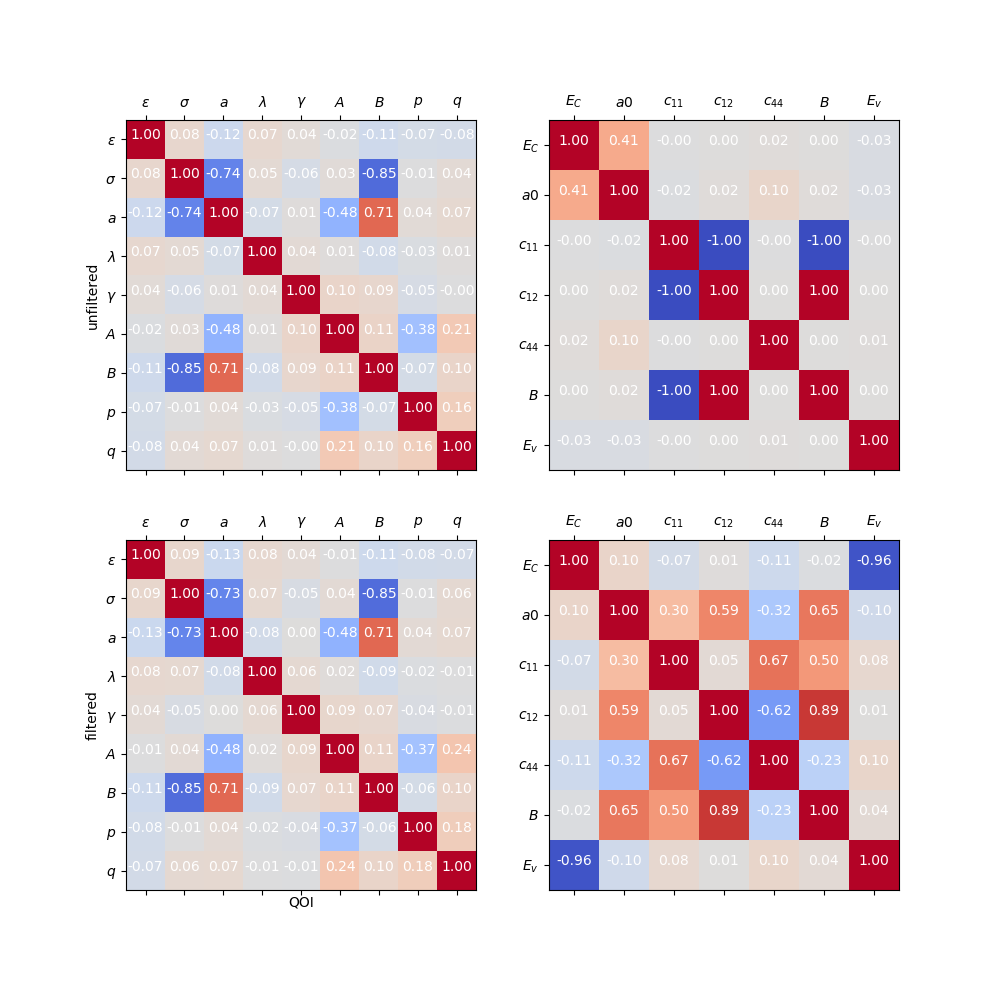
\includegraphics[width=5in]{chapter8/fig_cov_19}
  \caption{A correlation matrix plot with positively correlated variables indicated with a red gradient shader and negatively correlated variables indicated with a blue gradient shader.  Data comes from the $N=20$ iteration.  The left and right columns are the parameters and QOI relationships, respectively.  The top and bottom rows are unfiltered and filtered relationships, respectively.}
  \label{fig:Si_correlation_plots}
\end{figure}

\subsection{Bivariate Analysis}

A non-linear association between may exist between components, but this would not be described by the Pearson correlation coefficient; a property which should evident in this application since each $\hat{q}_i(\bm{\theta})$ is a function of the same realization of the random variable $\bm{\Theta}$.  However, the Pearson's correlation coeffient fails to identify anything but linear relationships.  One mechanism to overcome this problem is through the visual inspection of bivariate plots.  In our application, we augment the typical representation of the scattter plot with a gradient shader to reflect areas of higher density indicated by the kernel density estimate.  The bivariate plot projects the high dimensional space ($N_Q$ for QOI space, and $N_P$ for Parameter space) into the 2-dimensional subspace with basis vectors in the direction of the variables under analysis.  Visual inspection of bivariate scatterplots allows the sense of the bivariate distribution between two variables to identify any systemic relationship between two variables, such as curvilinear or multimodal behavior which cannot be captured by correlation statistics.

\begin{figure}[ht]
  \centering
  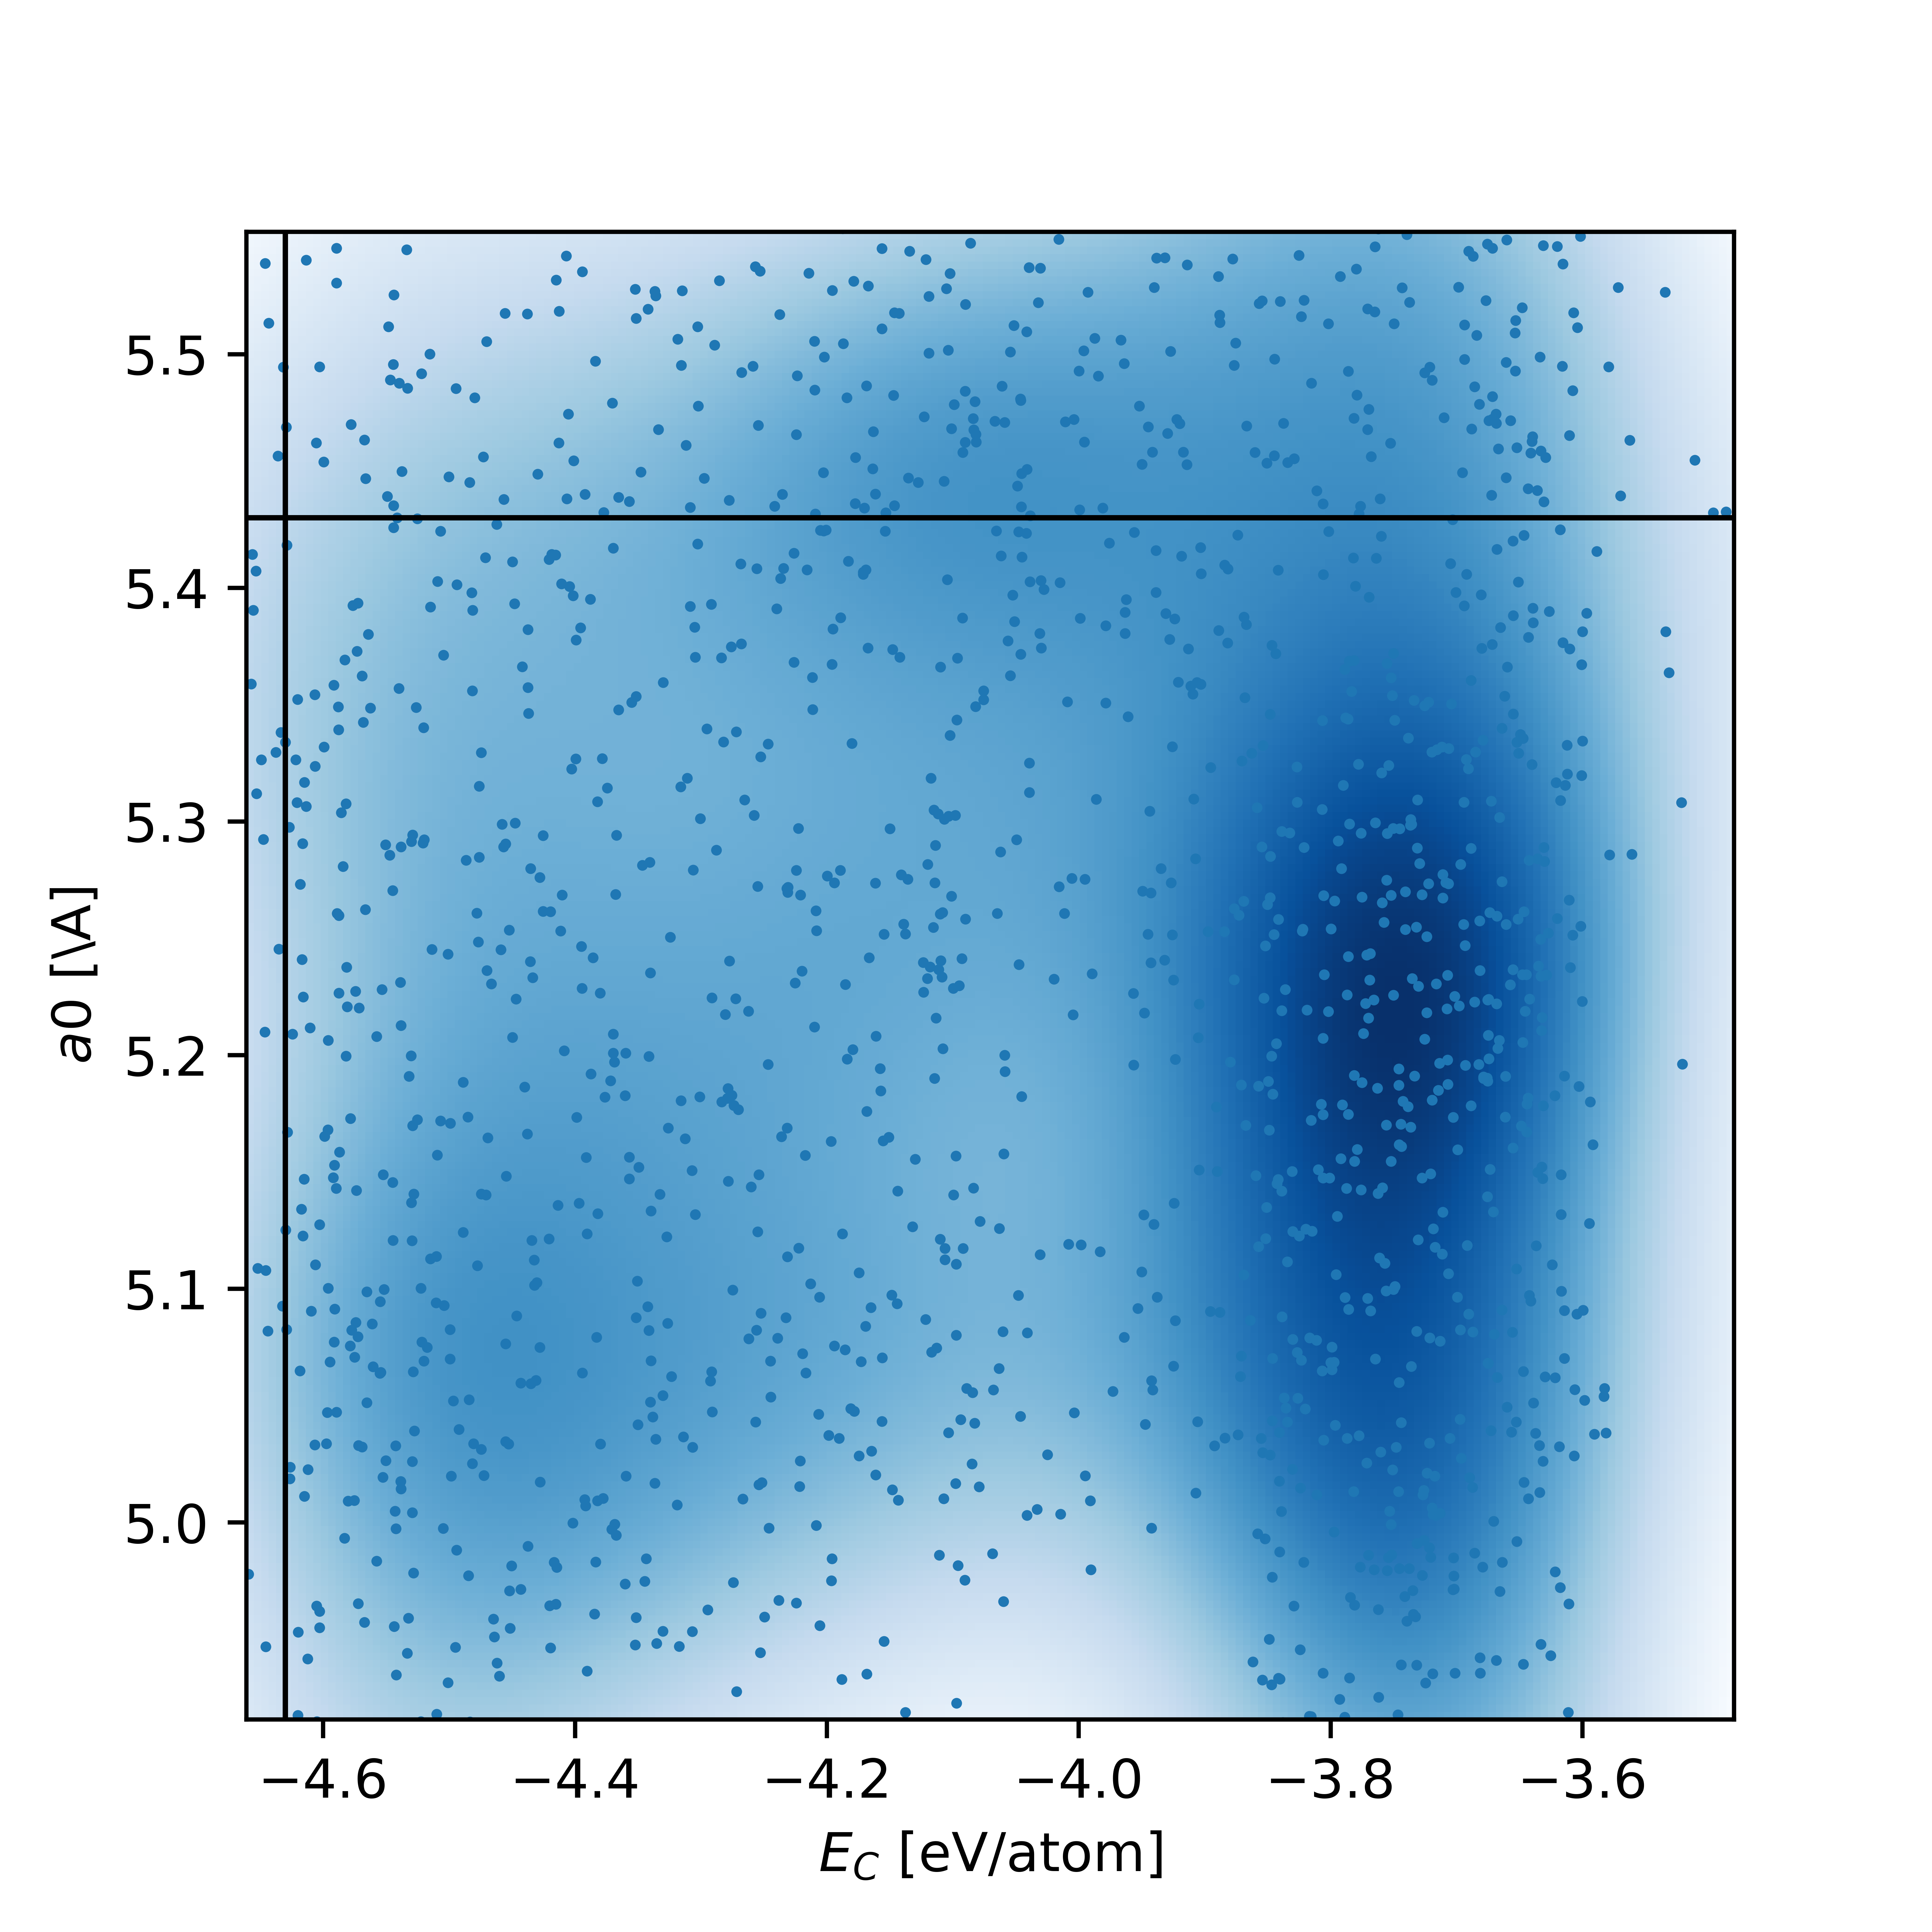
\includegraphics[width=5in]{chapter8/qoi_2d_density_plots/Si_dia_E_coh__Si_dia_a0}
  \caption{A bivariate plot of the predicted values for the cohesive energy $E_c$ against the lattice parameter $a_0$ for Si in diamond phase.  The dark lines indicated the target values for which the potential is optimized against}
  \label{fig:Si_Ec_a0_scatterplot}
\end{figure}

In the development of binary potentials, $E_c$ and $a_0$ given high weightings in the optimization process, so that simulations of interfaces, binary alloys, and binary phases.
In Figure \ref{fig:Si_Ec_a0_scatterplot}, a bivariate plot of the predicted values for the cohesive energy $E_c$ is plotted against the lattice parameter $a_0$ for silicon in diamond phase.
For reference, the target values for each QOI are also indicated on the plot.  Analysis of the scatter indicates a multi modal population with three regions of elevated probability density.
The primary region where of highest density located at $E_c=-3.86$ eV/atom and $a_0=5.22$ \AA, which is the region where most of the Pareto optimal potentials are located.  Two additional regions of elevated density closer to our QOI target values exist.  One closer to the target cohesive energy at $E_c=-4.5$ ev/atom and $a_0=5.05$ \AA.  The othe region is closer to the target lattice parameter value at $E_c=-4.1$ ev/Atom and $a_0=5.45$

The the number of parameters and the number of QOIs increases the number of bivariate plots increases expoentially, making the visual inspection of combinations tedious.    In addition, by projecting high dimensional data in low a low dimenstional subspace a considerable amount of information is lost in the process.  In addition, this approach is subjective, imprecise, and requires the potential developer to invest a significant amount of time in analysis to partition parameter space to refine the search to a specific area of interest.

\subsection{Gaussian Mixture Models in Two Dimensions}

Now we outline a technique for partitioning the Pareto optimal potentials, into subsets described by a normal distribution using Gaussian mixture models (GMM).  A GMM is a probabilistic model that assumes that all data points are generated from a mixture of a finute number of Gaussian distributions with unknown parameters.  Here we will partition the biobjective space formed by $a_0$ and $E_c$, for GMM analysis.

Before outlining the procedure for Gaussian Mixture Model in the general case, we motivate the use of the algorithm in the 2D case of two QOI variables based upon the previous example of $E_c$ and $E_v$ before moving to a general approach to partitioning the ensemble of Pareto optimal potentials.

A Gaussian mixture model (GMM) is part of the family of a Dirichlet processes, which are a probability distributions whose range are itself a set of probability distributions.\cite{west1994_mixturemodel}
Dirichlet processes are frequently used in Bayesian nonparameteric statistics, where nonparametric does not mean a parameter-less distribution, but rather a model in which the representations grow as more data is observed.
A GMM with with $K$ components can be written for the random variable $\bm{x}(\omega) \in \bm{X}(\Omega)$ with $\bm{x} \in \mathbb{R}^d$ as the sum of Gaussian distributions,
\begin{equation}
\label{eq:gmm}
  p_{\text{GMM}}(\bm{x}|
                 \bm{\mu}_1,...,\bm{\mu}_K,
                 \bm{\Sigma}_1,...,\bm{\Sigma}_K
                 \phi_1,...,\phi_K)
  =
  \sum_{k=0}^K \phi_k N(\bm{x}|\bm{\mu}_k,\bm{\Sigma}_k)
\end{equation}
where $\bm{\mu}_k$ are the means, $\bm{\Sigma}_k$ is the covariance matrix, $\phi_k$ is the mixing proportion ($0<\phi_k<1$ and $\sum_k \phi_k = 1$), and $N$ is a normal multivariate distribution function with the speciified mean and covariance matrix for the $k$th component of the GMM.

In order to choose the number of components which should include in a Gaussian mixture model we use a method based upon the calculation of information criteria (IC) described by Celeux and Soromenho\cite{celeux1996_gmm_components}.
ICs are estimator of the relative quality of statistical models for a given set of data, by penalizing potentials for using a more complicated model.
Here we base the number of clusters based upon the Akaike information criterion (AIC)\cite{akaike1998_aic} and the Bayesian information criterion (BIC) \cite{schwarz1978_bic}.
The AIC or BIC of a model is written in the form $[2\log(\hat{L}+kp]$, where $\hat{L}$ is a likelihood function, $p$ is the number of parameters in the model, and $k$ is $2$ for AIC and $\log(n)$ for BIC.
Given a collection of models for data, both the AIC and BIC estimate the quality of each model relative to the other models, providing a mechanism for model selection.
The \emph{scikit-learn} Python package\cite{pedregosa2011_scikitlearn} is used to fit the GMM for $1 < k < 20$ components and calculate the AIC and BIC with only $E_v$ and $a_0$ provided.
In Figure \ref{fig:Si_Ec_a0_aic_bic}, the BIC indicates that $4$ components should be used in the GMM model, while the AIC indicates are larger number of components should be used.
In a more thorough analysis, GMM models utilizing a number of components from a minimum to a maximum number of components would be examined based upon the different values provided by AIC vs BIC.
\begin{figure}[ht]
	\centering
	\includegraphics{chapter8/aic_bic_plot}
	\caption{Identification of the number of Gaussian components recommmended for a Gaussian mixture model for the biobjective space formed by the lattice parameter $a_0$ and the lattice parameter $a_0$.  Here, the BIC criteria indicates a smaller number of components, while AIC indicates that a larger number of components should be used.}
	\label{fig:Si_Ec_a0_aic_bic}
\end{figure}

The results for the GMM model with $K=4$ components is shown in Figure \ref{fig:Si_Ec_a0_gmm}.  The four different components aree indicated with ellipses and the potential points colored based upon their classification.  The locations of the different normal distributions and their associated weights are listed in Table \ref{tbl:sw_2parameter_gmm}.  In addition to the three clusters which we expected ($k=1,2,3$).  The fourth cluster ($k=4$) has a large variance which models the outliers.  The orientation of the elipses represents the orientation of the variance-covariance matrix, $\bm{\Sigma}_k$.
The centroid of the elipses for cluster $k$ is specificed by $\bm{\mu}_k$.  The length of the major and minor axis comes from a the eigenvalue-eigenvector decomposition of $\bm{\Sigma}_k$, a process known as principle components analysis (PCA).\cite{pearson1901_pca,hotelling1933_pca}.  The eigenvalues give the length of the major and minor axis and the associated eigenvectors provide the direction.  Since the eigenvetors are orthgonal to each other, PCA is a change of coordinates of the $\bm{\Sigma}$ so that linear vectors (the principle components) describe the orientation of the variance.

\begin{table}[ht]
	\centering
	\caption{Location information for each cluster, $k$  from a two dimensional GMM model consisting of the $E_c$ and $a_0$ components along with weighting $\phi$.}
	\label{tbl:sw_2parameter_gmm}
	\begin{tabular}{c c c c}
    \hline
    $k$ & $\phi$ & $E_c$ & $a_0$ \\
        &        & [eV]  & \AA   \\
    \hline
    1 & 0.28 & -3.72  & 5.12 \\
    2 & 0.36 & -4.43  & 5.18 \\
    3 & 0.27 & -3.93  & 5.38 \\
    4 & 0.08 & -4.09  & 5.34 \\
    \hline
  \end{tabular}
\end{table}

\begin{figure}[ht]
	\centering
	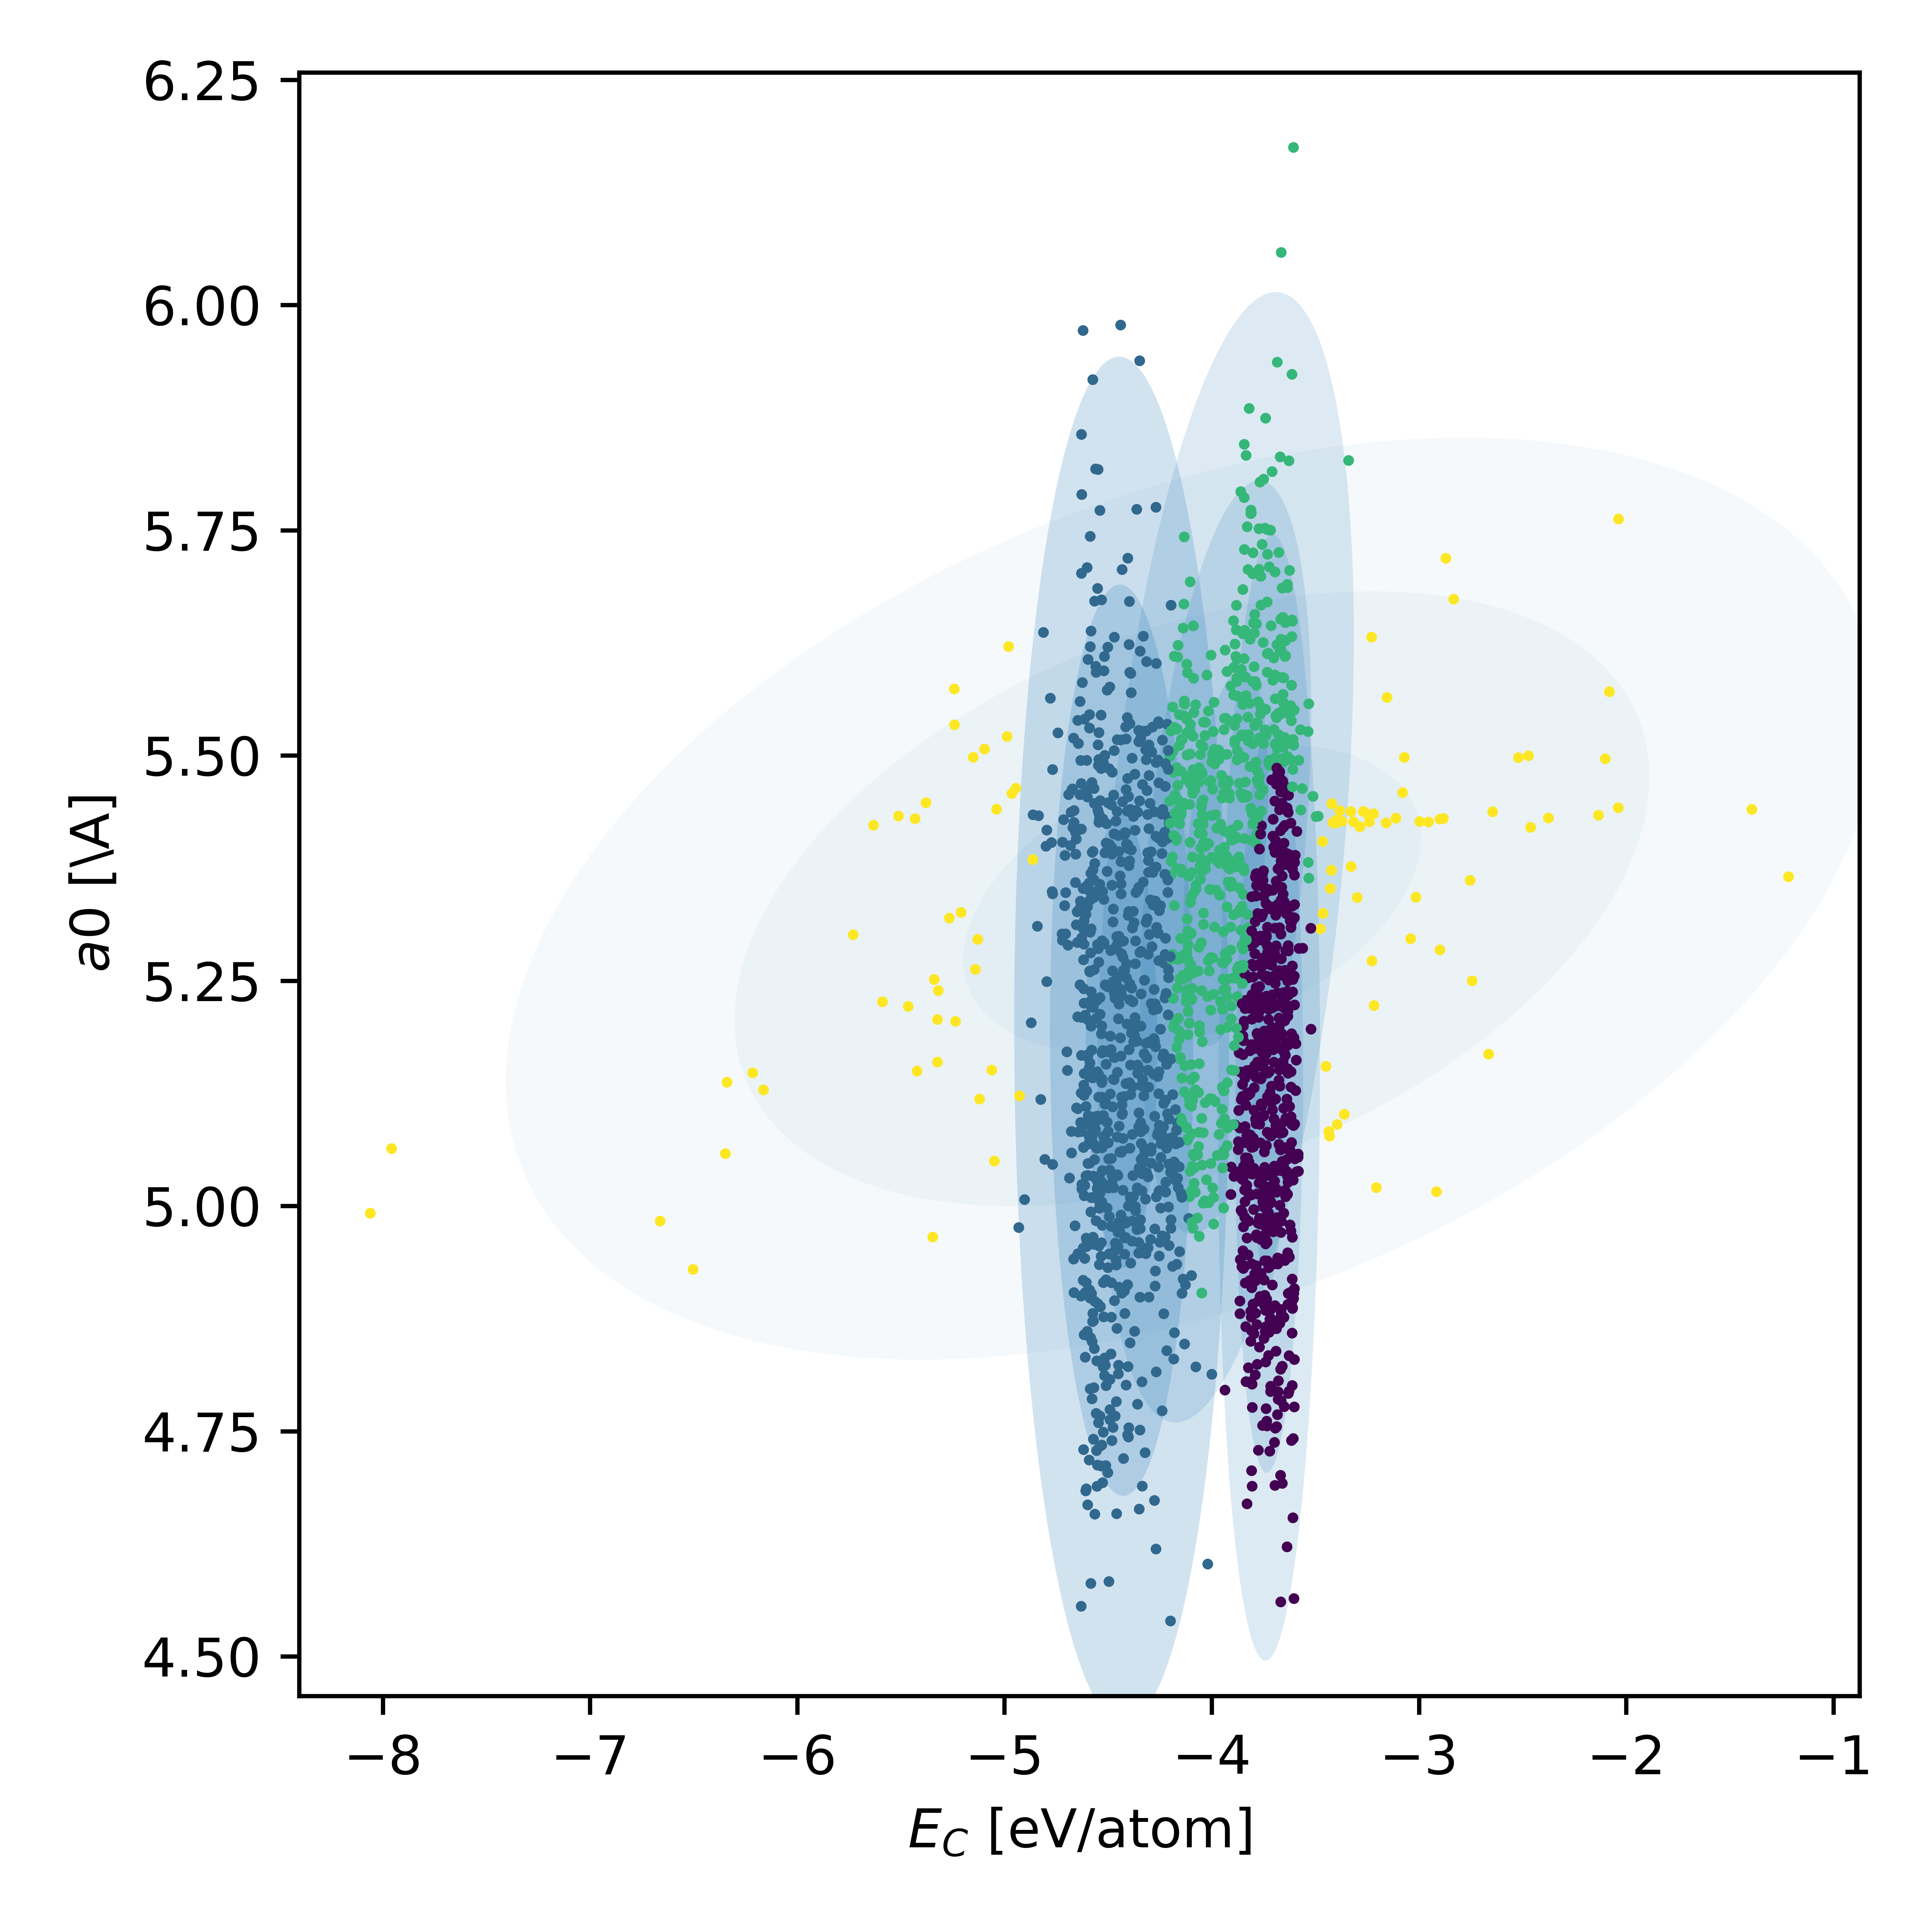
\includegraphics[width=5in]{chapter8/Si_Ec_a0_gmm}
	\caption{Application of the Gaussian mixture model with $K=4$ components.  Ellipses indicating direction and magnitude of the variances are indicated by the grey circles.}
	\label{fig:Si_Ec_a0_gmm}
\end{figure}

\begin{figure}[hbt]
	\centering
	\captionsetup{justification=centering,margin=1in}
	\includegraphics[width=5in]{chapter8/gmm_parallel_plot}
	\caption{Parallel plot}
	\label{fig:Si_gmm_parallel_plot_2_qoi}
\end{figure}

\subsubsection{A general approach to Gaussian mixture models}

We now generalize the approach from 2D case to an application more generally applicable to the potential development process.  As the size of the Pareto set grows, the selection of a potential becomes more difficult.  A GMM process can help partition to partition the set into similar potentials each defined by a normal distribution.  Rather than determine the indivial Gaussian components by analysis of parameter space of QOI space, we pass both the free parameters and the QOIs into the GMM model to ensure that clusters in QOI space produce cluster in parameter space.

To accomplish this, let us define the different components in Equation \ref{eq:gmm}.  Each data point is represented by a the vector $\bm{x}$,
\begin{equation}
\label{eq:gmm_input_vector_all}
    \bm{x} = (\theta_1,...,\theta_{N_P},\hat{q}_1,...\hat{q}_{N_Q})
\end{equation}
The mean for each component $k$ $\bm{\mu}_k$ has the same shape as $\bm{x}$,
\begin{equation}
\label{eq:gmm_output_mean_all}
    \bm{\mu} = (\theta_{k,1},...,\theta_{k,N_P},\hat{q}_{k,1},...\hat{q}_{k,N_Q})
\end{equation}
The variance covaraiance matrix from cluster $k$ then becomes
\begin{equation}
\label{eq:gmm_output_mean_all}
  \bm{\Sigma}_k
  = \left(
      \begin{array}{c|c}
        \bm{\Sigma}_{k,\bm{\theta},\bm{\theta}} & \bm{\Sigma}_{k,\bm{\theta},\bm{q}} \\
        \hline
        \bm{\Sigma}_{k,\hat{\bm{q}},\bm{\theta}}     & \bm{\Sigma}_{k,\bm{\hat{q}},\bm{\hat{q}}}
      \end{array}
    \right)
  = \left(
      \begin{array}{ccc|ccc}
           \Sigma_{k,\theta_1,\theta_1}  & \dots  & \Sigma_{k,\theta_1,\theta_{N_P}}
          &\Sigma_{k,\theta_1,\hat{q}_1} & \dots  & \Sigma_{k,\theta_1,\hat{q}_{N_Q}} \\
           \vdots                        & \ddots &
          &\vdots                        & \ddots & \\
           \Sigma_{k,\theta_{N_P},\theta_1} &     & \Sigma_{k,\theta_{N_P},\theta_{N_P}}
          &\Sigma_{k,\theta_{N_P},\hat{q}_1} &     & \Sigma_{k,\theta_{N_P},\hat{q}_{N_Q}} \\
        \hline
        \Sigma_{k,\hat{q}_{N_Q},\theta_{N_P}}  & \dots  & \Sigma_{k,\hat{q}_1,\theta_{N_P}}
       &\Sigma_{k,\hat{q}_1,\hat{q}_1} & \dots  & \Sigma_{k,\hat{q}_1,\hat{q}_{N_Q}} \\
        \vdots                        & \ddots &
       &\vdots                        & \ddots & \\
        \Sigma_{k,\hat{q}_{N_Q},\theta_1} &     & \Sigma_{k,\hat{q}_1,\theta_1}
       &\Sigma_{k,\hat{q}_{N_Q},\hat{q}_1} &     & \Sigma_{k,\hat{q}_{N_Q},\hat{q}_{N_Q}}
      \end{array}
    \right)
\end{equation}
where
$\Sigma_{k,\bm{\theta}, \bm{\theta}}$ is the covariance matrix for the parameters,
$\Sigma_{k,\hat{\bm{q}}, \hat{\bm{q}}}$ is the covariance matrix for the prediction of the parameters, and
$\Sigma_{k,\hat{\bm{q}}, \bm{\theta}}$ contains the covariance relationships between elements of $\hat{\bm{q}}$ and $\bm{\theta}$.

We evaluate GMM models for a large range of possible components ($1 \leq K \leq 100$) and calculate the AIC and BIC for each $K$.  The number of models to selected are determined using the same AIC and BIC criteria used in the 2D case with results shown in
Figure \ref{fig:Si_aic_bic_all}.  As expected with IC analysis, the AIC estimates a more coarse grained model ($\argmin_K(\text{AIC}_K) = 7$) and the BIC demands a greater number of components ($\argmin_K{\text(BIC)_K} = 57$).
A more coarse grained model here is selected to simplify the analysis with $K=10$, the weights and components for each model are indicated in Table \ref{tbl:sw_all_gmm}.

The structure $\bm{\mu}_k$ can be divided into $\bm{\mu}_{k,\bm{\theta}}$ and $\bm{\mu}_{k,\hat{\bm{q}}}$ which for each cluster $k$ provides the mean in both parameter space and QOI space.
Likewise, the $\Sigma_{k,\bm{\theta}, \bm{\theta}}$ and $\Sigma_{k},\hat{\bm{q}}, \hat{\bm{q}}$ blocks can be selected from $\bm{\Sigma}_k$ to get the representative covariance structure for each block.
Table \ref{tbl:sw_all_gmm_parameters} contains the mean ($\mu$) and standard deviation ($\sigma$) for the parameters in each representative distribution.  Table \ref{tbl:sw_all_gmm_qois} contains the mean ($\mu$) and standard deviation ($\sigma$) for the QOIs for each representative normal distribution.


\begin{figure}[hbt]
	\centering
	\captionsetup{justification=centering,margin=1in}
	\includegraphics[width=5in]{chapter8/aic_bic_all}
	\caption{AIC and BIC}
	\label{fig:Si_aic_bic_all}
\end{figure}

\begin{table}[ht]
	\centering
	\caption{Information for each cluster, $k$  for a full gmm model consisting of the $E_c$ and $a_0$ components along with weighting $\phi$.}
	\label{tbl:sw_all_gmm}
	\begin{tabular}{c c c}
    \hline
    id & $\phi$ & N\\
    \hline
    0 & 0.0110 & 22\\
    1 & 0.1644 & 328\\
    2 & 0.0267 & 53\\
    3 & 0.1897 & 380\\
    4 & 0.1599 & 325\\
    5 & 0.0105 & 21 \\
    6 & 0.0369 & 74 \\
    7 & 0.2124 & 427 \\
    8 & 0.0646 & 124 \\
    9 & 0.1238 & 2 \\
    \hline
  \end{tabular}
\end{table}

\begin{table}[ht]
	\centering
	\caption{QOI information for each constituent distribution, $k$, in the full GMM model.  The $\mu$ and $\sigma$ are provided for each $k$}
  \label{tbl:sw_all_gmm_parameters}
  \begin{tabular}{ccccccccccc}
    \hline
    $k$ & & $\epsilon$ & $\sigma$ & $a$ & $\lambda$ & $\gamma$ & $A$ & $B$ & $p$ & $q$\\
    \hline
    0 & $\mu$     & 2.1351 & 2.3293 & 1.6766 & 28.5357 & 0.8505 &  9.7152 & 0.5807 & 4.0951 & 0.8467\\
      & $\sigma$  & 0.0682 & 0.2669 & 0.1521 &  7.7997 & 0.1493 &  2.6653 & 0.2228 & 0.9456 & 0.3747\\
    1 & $\mu$     & 2.1490 & 1.9969 & 1.8311 & 25.4190 & 1.5878 &  9.9049 & 0.8331 & 3.6544 & 0.5476\\
      & $\sigma$  & 0.0483 & 0.1617 & 0.1310 &  5.7093 & 0.2308 &  2.2902 & 0.1882 & 0.5614 & 0.3108\\
    2 & $\mu$     & 2.1482 & 1.8758 & 1.8756 & 25.4777 & 1.0569 &  8.3311 & 0.7488 & 3.4368 & 0.5520\\
      & $\sigma$  & 0.0410 & 0.2431 & 0.1961 &  6.7885 & 0.1943 &  2.2901 & 0.2423 & 0.6626 & 0.3784\\
    3 & $\mu$     & 2.1561 & 1.9544 & 1.6951 & 25.9161 & 1.7207 & 13.9368 & 0.8124 & 3.6680 & 0.5712\\
      & $\sigma$  & 0.0448 & 0.1760 & 0.1372 &  6.1449 & 0.3639 &  3.5159 & 0.2045 & 0.6931 & 0.3485\\
    4 & $\mu$     & 2.1491 & 2.1281 & 1.7072 & 24.9994 & 1.9443 & 12.1992 & 0.7337 & 3.5037 & 0.5780\\
      & $\sigma$  & 0.0518 & 0.1678 & 0.1240 &  5.7167 & 0.3621 &  3.4780 & 0.1711 & 0.7115 & 0.3561\\
    5 & $\mu$     & 2.1534 & 2.1774 & 1.8049 & 24.6114 & 1.2441 &  9.7888 & 0.6525 & 3.7626 & 0.7401\\
      & $\sigma$  & 0.0459 & 0.2845 & 0.2144 &  4.9739 & 0.2580 &  5.1655 & 0.2673 & 0.8637 & 0.3980\\
    6 & $\mu$     & 2.1519 & 1.8270 & 1.7388 & 25.5017 & 1.5188 & 13.5491 & 0.8534 & 3.6855 & 0.5233\\
      & $\sigma$  & 0.0401 & 0.1428 & 0.1363 &  5.0800 & 0.4539 &  4.1506 & 0.2208 & 0.6263 & 0.3326\\
    7 & $\mu$     & 2.1476 & 2.0407 & 1.7857 & 26.4184 & 1.1863 & 10.5462 & 0.7723 & 3.6551 & 0.6172\\
      & $\sigma$  & 0.0483 & 0.1930 & 0.1426 &  5.1799 & 0.1745 &  2.7306 & 0.1956 & 0.6134 & 0.3709\\
    8 & $\mu$     & 2.1552 & 2.1884 & 1.7455 & 24.3617 & 1.6889 & 11.6354 & 0.7398 & 3.5336 & 0.6545\\
      & $\sigma$  & 0.0575 & 0.3587 & 0.2754 &  7.1845 & 0.4994 &  4.4585 & 0.3302 & 0.7927 & 0.3982\\
    9 & $\mu$     & 2.1468 & 1.9670 & 1.8592 & 27.0576 & 1.0078 &  9.5202 & 0.8099 & 3.6848 & 0.6391\\
      & $\sigma$  & 0.0513 & 0.1709 & 0.1485 &  4.9628 & 0.1745 & 2.9529 & 0.1818 & 0.6379 & 0.3468\\
    \hline
  \end{tabular}
\end{table}

\begin{table}[ht]
	\centering
	\caption{QOI information for each constituent distribution, $k$, in the full GMM model.  The $\mu$ and $\sigma$ are provided for each $k$}
  \label{tbl:sw_all_gmm_qois}
  \begin{tabular}{ccccccccc}
    \hline
    $k$ & & $E_C$ & $a0$ & $c_{11}$ & $c_{12}$ & $c_{44}$ & $B$ & $E_v$\\
        & & eV/atom & \AA & GPa & GPa & GPa & GPa & eV \\
    \hline
    0 & $\mu$     & -4.2055 & 5.4118 & 307.8981 & 32.6633 & 137.1558 & 124.4082 & 4.1974\\
     & $\sigma$   & 0.4038 & 0.1788 & 29.8008 & 37.9242 & 12.4975 & 21.3103 & 0.4044\\
    1 & $\mu$     & -4.0628 & 5.3496 & 133.2494 & 98.4785 & 30.5936 & 110.0688 & 4.0628\\
     & $\sigma$   & 0.3429 & 0.1804 & 26.3126 & 26.7241 & 11.3819 & 25.7962 & 0.3429\\
    2 & $\mu$     & -3.9872 & 4.9025 & 141.8443 & -15.6858 & 75.2049 & 36.8243 & 3.9836\\
     & $\sigma$   & 0.3966 & 0.2342 & 38.4908 & 18.0676 & 11.3542 & 14.7759 & 0.3963\\
    3 & $\mu$     & -4.0820 & 5.0081 & 129.9131 & 62.6440 & 57.2602 & 85.0670 & 4.0820\\
     & $\sigma$   & 0.3759 & 0.0822 & 24.9165 & 24.3370 & 13.0931 & 23.1579 & 0.3759\\
    4 & $\mu$     & -3.9786 & 5.3708 & 135.8375 & 121.2139 & 13.8574 & 126.0884 & 3.9786\\
     & $\sigma$   & 0.3800 & 0.1216 & 25.2843 & 22.3983 & 11.1543 & 22.7184 & 0.3800\\
    5 & $\mu$     & -4.5323 & 5.2940 & 159.4287 & 49.0808 & 71.8973 & 85.8634 & 3.6552\\
     & $\sigma$   & 1.7752 & 0.2127 & 32.4540 & 22.2257 & 17.1648 & 23.9528 & 1.7244\\
    6 & $\mu$     & -4.1263 & 4.7881 & 100.8331 & -1.9028 & 71.9410 & 32.3425 & 4.0772\\
     & $\sigma$   & 0.3745 & 0.0921 & 17.8274 & 11.3283 & 11.3778 & 10.9795 & 0.3816\\
    7 & $\mu$     & -4.1075 & 5.2920 & 166.8931 & 72.5505 & 69.1024 & 103.9980 & 4.1075\\
     & $\sigma$   & 0.5248 & 0.2041 & 35.2261 & 26.5453 & 15.3744 & 27.3971 & 0.5248\\
    8 & $\mu$     & -4.1252 & 5.3739 & 123.7958 & 89.8818 & 26.4300 & 101.1865 & 4.1252\\
     & $\sigma$   & 0.3735 & 0.2946 & 39.4293 & 39.0031 & 29.7312 & 35.5491 & 0.3734\\
    9 & $\mu$     & -4.0385 & 5.2610 & 209.4494 & 26.7454 & 99.4384 & 87.6467 & 4.0385\\
     & $\sigma$   & 0.4629 & 0.2546 & 52.3615 & 26.9835 & 21.0676 & 28.7038 & 0.4629\\
    \hline
  \end{tabular}
\end{table}

\subsection{Applications}
In the Pareto optimization process, the Pareto surface is estimated by evolving a kernel density esimate (KDE).  Since the KDE is non-parametric, it overcomes the problems with parametric distribution, parametric distributions have the assumption of a unimodal distribution.  However, the KDE assumes the variance and covaraince a homoskedastic since the same bandwidth matrix is applied across the distributions.  The GMM models partitions the parameter space into populations that can then be described by the KDE with a bandwidth parameter particular to that KDE.

After convergence is met, the potential developer may want to identify more potentials in a region of interest.  The GMM models allows the developer to isolate and eliminate certain regions from consideration.  Since the probability density of $\bm{\theta}$ is localized to a particular region, the sampling intensity would increase easing the sampling demands to find a new Pareto optimal potential.

If $k$ is chosen to be sufficiently high, the variance of the parameters as well as the predicted QOI values becomes reduced, and the Normal distribution specified in parameter space could be used for feed forward Bayesian UQ methodologies since the calculation of the analytical form of likelihood function for the Normal distribution known.

\subsection{Evaluation of constituent GMM distributions}

Unlike Chapter \ref{ch:ionic_MgO}, our options here are no longer individual potentials but described by a normal probability distribution for each constituitive options.  For an empirical interatomic potentials where the mean $\mu_{k,\hat{\bm{q}}}$ is sufficently close to the the target QOI values.  A one sample Hotelling's $t$-squared squared ($t^2$) could be used.  However, since none of the distributions identified are likely to contain $\mu_{k,\hat{\bm{q}}}$
\begin{table}[ht]
\centering
\caption{$p$-value type scoring for each constituent distribution, $k$, in the full GMM model.  Each $q$ is tested to determine is in the normal distribution, $N(\bm{\mu}_{k,q},\bm{\Sigma_{k,q}})$
\label{tbl:sw_all_gmm_qois}
\begin{tabular}{ccccccccc}
\hline
$k$ & $E_C$ & $a0$ & $c_{11}$ & $c_{12}$ & $c_{44}$ & $B$ & $E_v$ & total \\
    & eV/atom & \AA & GPa & GPa & GPa & GPa & eV & \\
\hline
0 & 0.0046 & 0.2843 & 0.4365 & 0.4913 & 0.3572 & 0.4777 & 0.0001 & 0.9314\\
1 & 0.0000 & 0.0068 & 0.4811 & 0.4807 & 0.3515 & 0.4934 & 0.0000 & 0.9121\\
2 & 0.0000 & 0.0000 & 0.4935 & 0.4036 & 0.4852 & 0.3879 & 0.0073 & 0.9055\\
3 & 0.0001 & 0.0000 & 0.4768 & 0.4991 & 0.4472 & 0.4896 & 0.0003 & 0.9261\\
4 & 0.0000 & 0.0000 & 0.4812 & 0.4546 & 0.2975 & 0.4791 & 0.0044 & 0.8969\\
5 & 0.4876 & 0.0013 & 0.4975 & 0.4880 & 0.4890 & 0.4909 & 0.4926 & 0.9826\\
6 & 0.0002 & 0.0000 & 0.4188 & 0.3038 & 0.4752 & 0.2902 & 0.0005 & 0.8494\\
7 & 0.0289 & 0.0005 & 0.4997 & 0.4952 & 0.4816 & 0.4973 & 0.0327 & 0.9382\\
8 & 0.0001 & 0.2590 & 0.4892 & 0.4932 & 0.4758 & 0.4993 & 0.0001 & 0.9497\\
9 & 0.0029 & 0.0046 & 0.4937 & 0.4796 & 0.4825 & 0.4945 & 0.0204 & 0.9330\\
\hline
\end{tabular}
\end{table}






As the number of parameters and material properties involved in the fitting process increases, the use of bivariate plots and biobjective plots becomes more difficult.


\subsection{Validation of Potentials}
 % EAM POTENTIAL DEVELOPMENT
%\chapter{Techniques for Dimensionality Reduction}

In the development of empirical interatomic potentials (EIP), the natural dimensionality of the problem can be daunting.
The representation of the atomic structures, $\bm{R}$, also known as the configuration space.

\section{Potential}

The interatomic potential, $V$ can be represented in the Born-Oppenheimer approximation as a mapping between the configurational space of atoms, $\bm{X}$, onto the set of possible energies, $U$.
Since $V:\bm{X} \rightarrow U$, then we can denote this relation as, $V(\bm{x})$, to represent energy for a structure, and $V(\bm{X})$ as potential energy surface.

Since \emph{ab initio} calculations are computational expensive, empirical interatomic potentials, $\hat{V}$ which which are defined by formulae, are often used to simulate larger systems and large time scales.
If $\bm{\Theta}$ represents the feasible parameterizations for $\hat{V}$, then the vector of $P$ optimal parameters, $\bm{\theta}^{*} = (\theta_1^{*},...,\theta_P^{*})$, must be be contained within the feasible parameterization, $\bm{\theta}^{*} \in \bm{\Theta}$.
Since $\hat{V}:\bm{\Theta},\bm{X} \rightarrow U$, then it is clear that
\begin{align}
  V &= \hat{V} + \varepsilon \\
  V(\bm{x}) &= \hat{V}(\bm{x},\bm{\theta}) + \varepsilon(\bm{x},\bm{\theta})
\end{align}
where $\varepsilon$ is the residual difference between $V(\bm{x})$ and $\hat{V}(\bm{x})$
 are defined by formulae which are parameterized for a specific material system.  Using the hat notation to denote an estimate,   The set of optimal parameters, $\bm{\theta}^{*} = (\theta_1^{*},...,\theta_P^{*})$ for $P$ parameters

\section{Principal Components Analysis}



Principal component analysis (PCA) is a statistical procedure that uses an orthogonal transformation to convert a set of observations of possibly correlated variables into a set of values linearly uncorrelated variables called principal compoents.

Pearson[1] and Hotelling[2]
 % SI
%\chapter{SUMMARY OF WORK}

\section{General Implications}

\section{Future Work}

\section{Robustness of Potentials}
Sensitive analysis.  Many models use cutoff-radii as an additional parameter to be determined by the fitting process.  Because of the nature of the stacking fault, the GSF energy must depend upon non-nearest neighbor interactions.
However, a slight alteration of the cutoff-radius was found to have a dramatic impact on the behavior of EAM potentials by Zimmerman.%\cite{Zimmerman2000_Ni_gsf}.  
He sugests that parameterizeed models should be only slightly sensitive to a change of value for any of it's parameters.  High sensitivity indicates the possibility of unphysical behavior of a model.  This issue should be address when creating a potential to be used in simulations that involve stacking faults.
 % MACHINE LEARNING
%\chapter{SUMMARY OF WORK}
\label{ch:summary}

\section{Significant Contributions}
This work set out to present an emergent framework for the automated development of analytical potentials.  Here we summarize key contributions in this work.

In Chapter \ref{ch:potential_development}, a critical assessment of the conventional process for potential paramaterization was provided.  We identified already known weakness with the process, but presented them in a more rigorous way.  Using cardinal optimization techniques is inappropriate because conditions for convergence to a global solutions are not met.  Convergence to global minima can only be met if the process is repeated across a dense range of initial conditions in space of possible potential parameterizations, or if random sampling techniques are employed.  In addition, the cost function formulation is unable to identify regions in the predictive performance when the optimal performance region is convex.  This creates high sensitivity to encoded preferences in convex regions due to the existence of degenerate solutions.  Finally, the \emph{a priori} expression of weights is required to be encoded at the beginning of the process.

We introduce the concept of ordinal minimization to the field of potential development, where the solution to parameter optimization is not expressed in an arbitrary cost function, which serves as an artifical heuristic, but in ordinal terms where we calculate an indifference curve based upon the concept of Pareto optimality where each candidate parameterization is mutally non-dominated.  This formulation elminates problems of local minima, expression of \emph{a priori} expression of weights, only imposes the condition the preservation ordinality to measure losses with respect to individual material properties of interest, and can identify solutions in convex regions of performance space normally occluded to cardinal optimization methods.

When the optimal performance has convexity or discontinuities, we show that the computational efficiency of Monte Carlo sampling techniquqes provides an order of magnitude improvement in  numerical efficiency in estimating the Pareto optimal surface, while simultaneously providing an order of magnitude computational efficiency in the number of simulations required.  In addition, ordinal optimization uses independent sampling which by definition provides near linear scalability in the ability of the algorithm to use processors.

Chapter \ref{ch:methodology} builds upon those concepts.  The implementation of constraints both in the domain of potential parameter design variable and the predictive performance is difficult within a cardinal optimization context, since Karush-Kuhn-Tucker conditions are likely not met, and most certaintly cannot be proved.  Cardinal optimization techniques have the undesirable task of implementing a non-linear programming scheme based upon simulations which must be treated as black box functions.  Here, we presented a modified Monte Carlo technique which uses acceptance-rejection sampling to modify the the distribution of the random variable \emph{ex post}.  This technique is considerably more flexible as ordinal optimization schemes are based upon criteria which are only dependent upon expressing an inequality.  This technique starts with the expression of the epistemic uncertainty that a potential developer has respect the location of the desireable potential parameters, and updates it in a Bayesian manner using evidence generated from Monte Carlo sampling.  This defines a new evolutionary algorithm for potential optimization that applicable for any multi-objective optimization program.

Chapter \ref{ch:software} implements these concepts into software.  A new software code \emph{pypospack} was developed to provide a framework for optimizing interatomic potentials.  Here the implementation of potentials, simulation tasks, and material properties are decomposed as independent components in an object-oriented architecture.  The use of inheritance allows us to encapsulate implementation details such as process handling, parallelization, and workflow management.  In turn, this lowers the necessary effort and expertise to contribute to the project.  An application \emph{pyposmat} which uses the \emph{pypospack} software libraries is used to implement the methodology described in Chapter \ref{ch:methodology}, and is applied to specific material systems in Chapters \ref{ch:ionic_MgO} and \ref{ch:pareto_si}.

Chapter \ref{ch:ionic_MgO} demonstrates that our unsupervised algorithm can deliver similar performance as expert-developed potentials for the magnesium oxide ionic system.  However, our Pareto optimization strategy has the inverse problem of cardinal optimizaton.  While cardinal optimization produces too few solutions.  The Pareto optimization strategy produces too many.  To solve this problem, we apply biobjective visualization techniques which projects the high dimensional data into a series of two-dimensional subspace.  This allows us to identify the performance tradeoffs in a global bivariate sense.

Chapter \ref{ch:pareto_si} introduces classification algorithms to the set of candidate potentials.  In the potential develop of a Stillinger-Weber potential for silicon, a large number of potential parameterizations are identified.  The number of potentials is so large that visualization techniques fail.  Here we apply the Gaussian mixture model (GMM) to partition the population and select a much smaller number of components determined by calculating the information criteria, which penalizes the selection of a more complicated model that adds too many components to the GMM.  This produces clusters which can be described with analytical multi-variate normal distributions.  The Student's $t$-test is used to assess the predictive performance of each material property of each cluster, and aggregate test for the performance was constructed.  This provides an algorithmic method for eliminating clusters with undesirable predictive based upon a $p$-value statistical tests.

\section{Future Work}

This new methodology is promising, but recommendations for future work and improvements are now discussed.

In order to provide continual improvement of the Pareto surface, it is necessary to constantly remove candidate potentials.  This process defines a cardinal scoring functions then ranks the potentials eliminating the poorest performance with respect to this metric.  Here, we scale the absolute errors by the target values and eliminate the worst performers by varying the volume of a hypersphere in this scaled space until a desired percentile of the candidate potentials are contained within this hypersphere.  Here, the choice of scaling is somewhat arbitrary and approximate, but serves to scale the errors to the same order of magnitude.  However, this filter seems to govern the optimization process and should be studied further.

This process produces are large number of candidate parameterizations.  However, the analysis space is high dimensional both in the design space of the potential parameters as well as the response space of predictive performance.  Linear projections into a two-dimensional subspace results in the loss of data.  The ill-conditioning of the covariance matrix suggests variance reduction techniques could be performed using eigenvalue-eigenvector analysis using a process such as principle components analysis, to project into a lower dimensional subspace without sacrificing too much information loss.

In addition, the distribution of parameters and predicted material properties are likely clustered due the existence both convex and concave regions of the Pareto surface.  We have demonstrated that clustering techniques are promising, but methodologies to translate these results into potential selection and improved sampling techniques have not been adequately explored.

On the software wide, we implement a simple parellization scheme which partitions the sample space and each processor processes an equal number of potentials.  However, some parameterizations may take more time to produce a result than others.  This leads to some processors finishing before others.  A more efficient concurrency scheme could be implemented.

Currently, the calculation of the Pareto surface and the calculation of the bandwidth parameter using cross-valdiation techniques are computational limitations since these calculations are performed on a single processor which increases memory requirements and computational time.   Parallelization schmes for both these processes would improve scalability.

Our potential produces a large amount of data.  Currently, the sampling scheme only uses information about the location of Pareto optimal points in determining random variates.  However, since the Pareto surface is the performance envelope between feasible and infeasible space, the dominated potentials provide considerable information on where to direct sample dispersions.  In addition, \emph{pypospack} produces a large amount of structured information stored in flat files.  The interactivity in analysis can be improved by integrating this information into a database, which can ease workstation analysis requirements due to the considerable memory and input-output demands of analysis.

Finally, the methodology provided here is specifed in probabilistic terms to make it compatible with VVUQ techniques.  This goal has not been accomplished due to the inadequacies of the formalism of the interatomic potential.  The reduction of epistemic uncertainty when performance tradeoffs are large implies a high degree of uncertainty in distribution of the potential parameters.  The modification of standard VVUQ techniques are necessary to deal with the inevitable biases when selecting a region of parameterization, particularly when dealing with propagating parametric uncertainty to dynamic simulations.
 % CONCLUSION
%\appendix{Calculation of Point Defect Energies}

This appendix documents the heuristics and algorithms for the automation for the calculation of point defects.
In theory, point defect calculations are dependent upon the interatomic cutoff of the interatomic potential.
However, the energies of pair-wise interactions vanish quickly due to tails of power-law and expoential distribution functions.
The author has found it instructive that even when the targets of the fitting database are taken from literature, \emph{ab initio} calculations to understand how large the size that the representative volume should be to prevent defect interaction
\section{Calculation of Point Defects}
In ionic materials, the formation of energy of a defect $d$ with charge $q$ is calculated as
\begin{equation}
  E_d^f=E_{def}-E_{perf}=\sum_\alpha n_\alpha \mu_\alpha - q\mu_e + E_{chcor} + E_elcor
\end{equation}
A point defect occur at or around a lattice point, there are not expanded into space in any direction.

A vacancy are lattice sites which would be occupied in a single crystal, but are vacant.  The stability of surrounding crystal structure prevents the atoms from occupying the vacancy.

In an ionic solid, the combination of a two vacanies of a cation and anion species are refrred to as a Schottky defect, which is neutral in nature.

A popular way to calculate defect energies from first principles or empirical potentials is based on the supercell idea.
In this method, the atoms in a unit cell are replicated by extending them in one or more directions in the direction of the translational symmetry operators defined by the basis vectors of the unit cell.
This enlarged area, known as the supercell, becomes the new representative unit cell of the system, and typically periodic boundary conditions are apply applied at it's borders.
The supercell method is one of three main approaches to defect calculations.  In finite cluste methods, the defect is simply incorporated into bulk material of finite exist, and ensure that the cluster is large enough to prevent to prevent surface effects.
Embedding techniques match the defect region to the known DFT Green's function of the ideal host material.  However, the numerical implementation of Greens func method is challenging as it requires well-localized defect potential and usually short-range basis functions.  The great advantage of supercell calculations is that the periodic boundary condition

The drawback to supercelll methods for defect calculations is that periodicity is artificial, and self-interaction of the defect.
For a more detailed discussion of supercell methods in DFT, the reader is encouraged to read Nieminen \cite{nieminen2007supercell}.
\section{Creation of Supercell}
The technique for creating supercell
\subsection{Definition of the defect in supercell calculation}

\subsection{Convergence conditions}
To ensure that convergence
\section{Future Work}

\section{Robustness of Potentials}
Sensitive analysis.  Many models use cutoff-radii as an additional parameter to be determined by the fitting process.  Because of the nature of the stacking fault, the GSF energy must depend upon non-nearest neighbor interactions.
However, a slight alteration of the cutoff-radius was found to have a dramatic impact on the behavior of EAM potentials by Zimmerman.%\cite{Zimmerman2000_Ni_gsf}.
He sugests that parameterizeed models should be only slightly sensitive to a change of value for any of it's parameters.  High sensitivity indicates the possibility of unphysical behavior of a model.  This issue should be address when creating a potential to be used in simulations that involve stacking faults.

%\appendix{Stress and Strain}
Stress is defined a a force applied to an area, $\sigma = F/\ell^2$

\section{Elastic Tensor Notation}

The theory of elasticity is a generalization of Hooke's law which relates the force $F$ needed to extend or compress a spring scales linearly with the spring constant  $k$, and the change in the length of spring $\Delta x$.  Put together, Hooke's law states

\begin{equation}\label{eq:hooke_law}
    \bm{F} = -k \Delta x
\end{equation}
with the negative sign implying that restorive force is produced by the spring is in the direction opposite of $\bm{F}$.


To generalize Hookes law for application to solids, the force applied is a applied to vanishing small surface. There are nine components to the stress applied to a body as represented in the schematic\ref{fig:stress_tensor}, referred to as the Cauchy stress tensor\cite{timeshenko1970_elasticity},
\begin{equation}
  \sigma_{ij}
  =
  \begin{pmatrix}
    \sigma_{11} & \sigma{12} & \sigma{13} \\
    \sigma_{21} & \sigma{22} & \sigma{23} \\
    \sigma_{31} & \sigma{32} & \sigma{33}
  \end{pmatrix},
\end{equation}

\begin{figure}[h]
  \includegraphics{appendixB/stress_tensor}
  \caption{Depiction of the components of the stress tensor}
  \label{fig:stress_tensor}
  \centering
\end{figure}

In figure \ref{fig:stress_tensor}, the faces of the representational solid are oriented to the normal vectorwhere the normal stress, $\sigma_{ii}$.  The Cauchy stress tensor, $\sigma_{ii}$, applied normal to the $\bm{e}_1$, is a normal pressure load.  Since the deformations are smalll then
\begin{equation}
  \sigma_{ii}=
\end{equation}

For a static body, the components of the Cauchy stress tensor in every material point in the body satisfies the Cauchy equations of motion for zero acceleration\cite{timeshenko1970_elasticity}, and the conservation of angular momentum implies that $\sigma_{ij}=\sigma{ji}$.

\begin{equation}
  \sigma_{ij} = C_{ijkl}\epsilon_{kl}
\end{equation}
where $\sigma_{ij}$ is the second order pressure tensor, and $\epsilon{kl}$ is a second order strain tensor.
$C_{ijkl}$ are the components of the fourth-order stiffness tensor of the material properties.  For three dimensions the fourth order has 81 components.

%\appendix{Pareto Optimization Problem}
\label{ap:pareto optimization_test}

Test function provide an artificial functional landscape which are useful to evaluate the characteristics of optimization algorithms for properties such as convergence rate, precision, robustness, and general performance.

The first of the test optimization function of a smooth convex multi-objective optimization problem described by Schaffer\cite{schaffer1984_pareto}.  Here the multi-objective function $F:\mathbb{R} \rightarrow \mathbb{R}^2$.
\begin{equation}
\begin{aligned}
  &\min_{x}
      \begin{aligned}
           &f_1(x) = x^2 \\
           &f_2(x) = (x-2)^2 \\
      \end{aligned}
\end{aligned}
\end{equation}

The second of the test optimization function is a discontinuous convex mutli-objective optimization problem described by Kursawe \cite{kursawe1991_pareto}.
\begin{equation}
\begin{aligned}
  &\min_{\bm{x}}
    \begin{aligned}[t]
      &f_(\bm{x}) = \sum_{i=1}^2
          \left[
            -10 \exp\left(-0.2 \sqrt{x_i^2} + x_{i+1^2}\right)
          \right] \\
      &f_x(\bm{x}) = \sum_{i=1}^3 \left[ \vert|x_{i} \vert|^{0.8} + 5\sin(x_i^3)\right] \\
    \end{aligned}
  &\text{subject to} \\
    \begin{aligned}[t]
      &-5 \leq x_i \leq -5 \\
      & 1 \leq i \leq 3 \\
    \end{aligned}
  \end{aligned}
\end{equation}
 % test pareto problems
%-----------------------------------------------------------------------%

% Use the appropriate file depending upon the number of appendices you have
%% The Editorial Office Requirements for the Table of Contents cause a significant problem
%in Latex if there is only one Appendix. The Appendix is no longer labeled "A" in the TOC
%but has the word "APPENDIX" placed in front of the title of the Appendix. This can be done
%without issue IF nothing needs to be numbered by LaTeX in the Appendix. Unfortunately, most of the time
%something needs to be numbered in that single Appendix. For this reason we have included the IFTHENELSE switch
%found in this document and at the beginning of AppendixA. We assume that if you have any appendices, that you have more than one. However, you DO only have one appendix DO NOT USE THIS FILE!!!!!!!!!!!!!!!!!!!!!!!
%
% OneSingleAppendix.tex has all the settings needed to adjust for a single appendix
% you will have a major problem with your TOC if you use this file with a single appendix!!!!!

%
% Comment (or delete) all of the \input{AppendixB} commands except those you are using.
%Then open the AppendixA.tex file and continue there.

%you can add/substract individual appendices through by using the /include{appendix'X'}
% and creating/deleting the appropriate files
\appendix %
%\clearpage%

\addtocontents{toc}{\protect\addvspace{10pt}\noindent{APPENDIX} \protect\hfill\par}{}


% % % % % % % If you have a single appendix, you should be using appendix1.tex
% % % % % % % NOT this file

\chapter{THIS IS THE FIRST APPENDIX}

Lorem ipsum dolor sit amet, consectetuer adipiscing elit. Maecenas
eget magna. Aenean et lorem. Ut dignissim neque at nisi. In hac
habitasse platea dictumst. In porta ornare eros. Nunc eu ante. In
non est vehicula tellus cursus suscipit. Proin sed libero. Sed risus
enim, eleifend in, pellentesque ac, nonummy quis, nulla. Phasellus
imperdiet libero nec massa. Ut sapien libero, adipiscing eu,
volutpat porttitor, ultricies eget, nisi. Sed odio. Suspendisse
potenti. Duis dolor augue, viverra id, porta in, dignissim id, nisl.
Vivamus blandit cursus eros. Maecenas sit amet urna sit amet orci
nonummy pharetra.

Praesent cursus nibh et mauris. In aliquam felis sit amet ligula.
Nulla faucibus nisl eget nisl. Aliquam tincidunt. Mauris eget elit
sed massa luctus posuere. Pellentesque suscipit. In odio urna,
semper ut, convallis ut, porta et, nibh. Nulla sodales metus nec
velit posuere gravida. Cras tristique. Etiam urna risus, accumsan
ut, placerat sed, iaculis id, est.

Nullam mi. Pellentesque habitant morbi tristique senectus et netus
et malesuada fames ac turpis egestas. Duis vitae metus in massa
hendrerit rhoncus. Fusce tortor justo, laoreet eu, facilisis at,
gravida et, felis. Donec imperdiet mollis erat. Integer tempus nulla
ac lorem. Fusce porttitor. Aenean quis arcu. Morbi consectetuer, leo
eu mollis elementum, urna massa malesuada risus, euismod tempor
lorem elit ut mauris. Cras elit orci, facilisis ac, mattis iaculis,
cursus ac, augue. Donec eget nisl. Pellentesque fermentum sodales
nibh. Vivamus non risus. Donec est libero, tincidunt sit amet,
pretium vitae, blandit sed, tellus. Nunc diam risus, interdum sed,
laoreet quis, varius ac, turpis. In et purus eget nibh vehicula
rhoncus. Aenean et neque. Praesent nisl nisi, tempus quis, nonummy
ac, auctor a, neque. Suspendisse et metus. Suspendisse non metus eu
mauris auctor sagittis.
 %
\chapter{AN EXAMPLE OF A HALF TITLE PAGE}%
\label{appendixB}

\clearpage %remove this command if your appendix doesn't start with a landscaped page!!!!!
\thispagestyle{plain}
\begin{landscape}
\begin{figure}

  \begin{center}
    \includegraphics[width=6in]{images/LaTeX2e_logo.eps}
    \caption{\LaTeX 2\ensuremath{\epsilon.} logo}\label{biglogo}
  \end{center}
\end{figure}
\end{landscape}


This is how a section should look if the first page is a landscape page.
Lorem ipsum dolor sit amet, consectetuer adipiscing elit. Ut sit
amet nulla. Integer mauris turpis, dapibus ac, auctor non, vehicula
sit amet, magna. Suspendisse eu tellus. Etiam porta. Donec magna.
Donec ut dui. In hac habitasse platea dictumst. Nullam suscipit, mi
at adipiscing commodo, lorem erat scelerisque erat, non pulvinar leo
mi eu metus. Phasellus id felis. Sed quam purus, molestie quis,
ultrices nec, dictum at, magna. Proin viverra viverra ante.

Maecenas sagittis magna quis ligula. Duis vestibulum mi a felis.
Aenean accumsan mattis massa. Nullam lacus sem, consectetuer non,
condimentum sit amet, pharetra ac, odio. Morbi nisi magna, tincidunt
sed, placerat nec, tincidunt id, lectus. Donec ac dui non mauris
vulputate aliquam. Nullam scelerisque congue pede. Integer ipsum.
Vestibulum auctor. Suspendisse eget leo id libero cursus dictum. Sed
malesuada. Aliquam imperdiet. Donec dui metus, porta eu, aliquet
vel, vulputate vitae, lacus.

Nulla quis purus id turpis luctus feugiat. Fusce feugiat. Proin
felis. Morbi elit est, fermentum in, tincidunt vitae, convallis vel,
orci. Vestibulum justo. Suspendisse non nisl. Pellentesque pretium
adipiscing elit. Phasellus fermentum consequat augue. Sed pede nisl,
fermentum vel, vulputate id, sollicitudin sed, ligula. Cras
suscipit, quam et euismod sagittis, nisl felis gravida felis, quis
pulvinar purus est vel pede. Suspendisse mattis est ac nunc.
Curabitur rutrum, turpis sit amet commodo tempus, metus lorem
commodo lectus, eget fringilla justo nisi et purus. Ut quam sapien,
vehicula quis, rhoncus non, sagittis nec, risus.

Donec eget augue ac lacus adipiscing porta. Maecenas pede. Vivamus
molestie. Duis condimentum ligula auctor pede. Nullam ullamcorper
rhoncus erat. Ut ornare interdum urna. Suspendisse potenti.
Curabitur mattis mauris nec risus. Aenean iaculis turpis eu tortor.
Donec nec ante non mauris pellentesque fringilla.

Phasellus vitae dui id orci sodales cursus. Curabitur sed nulla quis
mauris tincidunt iaculis. Vivamus semper semper orci. Phasellus
suscipit ante vitae leo. Sed arcu ipsum, condimentum id, luctus in,
sodales eu, magna. In dictum, arcu quis pharetra vestibulum, ante
enim placerat lacus, vitae placerat est leo vitae elit. Pellentesque
bibendum enim vulputate eros. Nunc laoreet. Pellentesque habitant
morbi tristique senectus et netus et malesuada fames ac turpis
egestas. Praesent purus odio, euismod sit amet, aliquam a, volutpat
in, augue. Phasellus id massa. Suspendisse suscipit ligula pharetra
dolor. Pellentesque vel pede.

Aliquam pharetra est sit amet magna. Aliquam varius. Donec eu lectus
et nisl iaculis porttitor. Morbi mattis, mauris sed luctus
hendrerit, nulla velit molestie dolor, ac volutpat urna augue vel
quam. Maecenas pellentesque libero et massa. Integer vestibulum,
lacus at mattis euismod, nisl arcu commodo lectus, ut euismod dolor
ligula sit amet libero. Nam in ligula sit amet ante eleifend
aliquet. Phasellus feugiat erat at nulla. Proin in lectus. Proin
laoreet leo laoreet leo congue lacinia. Quisque non diam sit amet
enim ultrices commodo. Praesent fermentum lectus sed ligula. Integer
pulvinar accumsan pede. Quisque molestie ligula eget odio.
Vestibulum ante ipsum primis in faucibus orci luctus et ultrices
posuere cubilia Curae;
 %
\chapter{DERIVATION OF THE $\Upsilon$ FUNCTION}%
\label{appendixC}

%\clearpage %remove this command if your appendix doesn't start with a landscaped page!!!!!
%\thispagestyle{plain}
%\begin{landscape}
%\begin{figure}

 % \begin{center}
  %  \includegraphics[width=6in]{LaTeX2e_logo.eps}
   % \caption{\LaTeX 2\ensuremath{\epsilon.} logo}\label{biglogo}
  %\end{center}
%\end{figure}
%\end{landscape}

%%%%%%%%%%%%%%%%%%%%%%%%%%%%%%%%%%%%%%%%%%%%%%%%%%%%%%%%%%%%%%%%%%%%%%%%%%%%%%%%%%%%%%%%%%%%%%%%%%


%ADD LABEL

%%%%%%%%%%%%%%%%%%%%%%%%%%%%%%%%%%%%%%%%%%%%%%%%%%%%%%%%%%%%%%%%%%%%%%%%%%%%%%%%%%%%%%%%%%%%%%%%%%

\proposition{The Upsilon Function}

(1) If $\beta>0$ and $\alpha\neq0$, then for all $n\geq-1$,

$$I_{n}(c;\alpha; \beta; \delta) = - \frac{e^{\alpha c}}{\alpha} \sum_{i=0}^{n}(\frac{\beta}{\alpha})^{n-i} Hh_{i}(\beta c -\delta)$$

$$+ (\frac{\beta}{\alpha})^{n+1} \frac{\sqrt{2 \pi}}{\beta} e^{\frac{\alpha \delta}{\beta}+\frac{\alpha^{2}}{2\beta^{2}}} \phi(-\beta c + \delta + \frac{\alpha}{\beta})$$
(2) If $\beta<0$ and $\alpha<0$, then for all $x \geq -1$

$$I_{n}(c;\alpha; \beta; \delta) = - \frac{e^{\alpha c}}{\alpha} \sum_{i=0}^{n}(\frac{\beta}{\alpha})^{n-i} Hh_{i}(\beta c -\delta)$$

$$- (\frac{\beta}{\alpha})^{n+1} \frac{\sqrt{2 \pi}}{\beta} e^{\frac{\alpha \delta}{\beta}+\frac{\alpha^{2}}{2\beta^{2}}} \phi(\beta c - \delta - \frac{\alpha}{\beta})$$

\begin{proof}{Case 1.}

$\beta>0$ and $\alpha\neq0$. Since, for any constant $\alpha$ and $n \geq 0$, $e^{\alpha x} Hh_{n}(\beta x - \delta) \rightarrow 0$ as $x \rightarrow \infty$ thanks to (B4), integration by parts leads to

$$I_{n}=-\frac{1}{\alpha}Hh(\beta c -\delta) e^{\alpha c} + \frac{\beta}{\alpha}\int_{c}^{\infty} e^{\alpha x} Hh_{n-1}(\beta c - \delta)dx$$

In other words, we have a recursion, for $n \geq 0$, $I_{n}=-(e^{\alpha c}{\alpha})Hh_{n}(\beta c - \delta) + (\frac{\beta}{\alpha})I_{n-1}$ with

$$I_{-1}=\sqrt{2 \pi} \int_{c}{\infty}e^{\alpha x}\varphi(-\beta x +\delta)dx$$

$$=\frac{\sqrt{2 \pi}}{\beta} e^{\frac{\alpha \delta}{\beta}+\frac{\alpha^{2}}{2 \beta^{2}}}\phi(-\beta c + \delta +\frac{\alpha}{\beta})$$

Solving it yields, for $n \geq -1$,

$$I_{n}=-\frac{e^{\alpha c}}{\alpha}\sum_{i=0}^{n}(\frac{\beta}{\alpha})^{i}Hh_{n-i}(\beta c+\delta) + (\frac{\beta}{\alpha})^{n+1}I_{-1}$$

$$=-\frac{e^{\alpha c}}{\alpha}\sum_{i=0}^{n}(\frac{\beta}{\alpha})^{n-i} Hh_{i}(\beta c+\delta)$$

$$+ (\frac{\beta}{\alpha})^{n+1}\frac{\sqrt{2 \pi}}{\beta} e^{\frac{\alpha \delta}{\beta}+\frac{\alpha^{2}}{2 \beta^{2}}}\phi(-\beta c + \delta +\frac{\alpha}{\beta})$$

where the sum over an empty set is defined to be zero.
\end{proof}

Case2. $\beta<0$ and $\alpha<0$. In this case, we must also have, for $n \geq 0$ and any constant $\alpha<0, e^{\alpha x}Hh_{n}(\beta x -\delta) \rightarrow 0$ as

$x \rightarrow \infty$, thanks to (B5). Using integration by parts, we again have the same recursion, for $n \geq 0, I_{n}=-(e^{\alpha c}/\alpha)Hh_{n}(\beta c - \delta)+(\beta / \alpha)I_{n-1}$, but with a different initial condition

$$I_{-1}=\sqrt{2 \pi}\int_{c}^{\infty}e^{\alpha x}\varphi(-\beta x + \delta)dx$$

$$=-\frac{\sqrt{2 \pi}}{\beta} exp\{\frac{\alpha \delta}{\beta}+\frac{\alpha^{2}}{2 \beta^{2}}\}\phi(\beta c - \delta -\frac{\alpha}{\beta})$$

Solving it yields (B8), for $n \geq -1$.

Finally, we sum the double exponential and the normal random variables

Proposition B.3.

Suppose $\{\xi_{1},\xi_{2},...\}$ is a sequence of i.i.d. exponential random variables with rate $\eta>0$, and Z is a normal variable with distribution $N(0,\sigma^{2})$. Then for every $ n \geq 1$, we have: (1) The density functions are given by:

$$f_{Z+\sum_{i=1}^{n}\xi_{i}}(t)=(\sigma\eta)^{n}\frac{e^{(\sigma\eta)^{2}/2}}{\sigma\sqrt{2\pi}}e^{-t\eta}Hh_{n-1}(-\frac{t}{\sigma}+\sigma\eta)$$

$$f_{Z-\sum_{i=1}^{n}\xi_{i}}(t)=(\sigma\eta)^{n}\frac{e^{(\sigma\eta)^{2}/2}}{\sigma\sqrt{2\pi}}e^{-t\eta}Hh_{n-1}(\frac{t}{\sigma}+\sigma\eta)$$
(2) The tail probabilities are given by

$$P(Z+\sum_{i=1}^{n}\xi_{i}\geq x) = (\sigma\eta)^{n}\frac{e^{(\sigma\eta)^{2}/2}}{\sigma\sqrt{2\pi}}e^{-t\eta}I_{n-1}(x;-\eta,-\frac{1}{\sigma},-\sigma\eta)$$

$$P(Z-\sum_{i=1}^{n}\xi_{i}\geq x) = (\sigma\eta)^{n}\frac{e^{(\sigma\eta)^{2}/2}}{\sigma\sqrt{2\pi}}e^{-t\eta}I_{n-1}(x;\eta,\frac{1}{\sigma},-\sigma\eta)$$

Proof. Case 1. The densities of $Z+\sum_{i=1}^{n}\xi_{i}$, and $Z-\sum_{i=1}^{n}\xi_{i}$. We have

$$f_{Z+\sum_{i=1}^{n}\xi_{i}}(t)=\int_{-\infty}^{\infty}f_{\sum_{i=1}^{n}\xi_{i}}(t-x)f_{Z}(x)dx$$

$$=e^{-t\eta}(\eta^{n})\int_{-\infty}{t}\frac{e^{x\eta}(t-x)^{n-1}}{(n-1)!}\frac{1}{\sigma\sqrt{2\pi}}e^{-x^{2}/(2\sigma^{2})}dx$$

$$=e^{-t\eta}(\eta^{n})e^{(\sigma\eta)^{2}/(2)}\int_{-\infty}{t}\frac{(t-x)^{n-1}}{(n-1)!}\frac{1}{\sigma\sqrt{2\pi}}e^{-(x-\sigma^{2}\eta)^{2}/(2\sigma^{2})}dx$$

Letting $y=(x-\sigma^{2}\eta)/\sigma$ yields

$$f_{Z+\sum_{i=1}^{n}\xi_{i}}(t)=e^{-t\eta}(\eta^{n})e^{(\sigma\eta)^{2}/(2)}\sigma^{n-1}$$

$$\times\int_{-\infty}^{t/\sigma-\sigma\eta}\frac{(t/\sigma - y -\sigma\eta)^{n-1}}{(n-1)!}\frac{1}{\sqrt{2\pi}}e^{-y^{2}/2}dy$$

$$=\frac{e^{(\sigma\eta)^{2}/2}}{\sqrt{2\pi}}(\sigma^{n-1}\eta^{n})e^{-t\eta}Hh_{n-1}(-t/\sigma + \sigma\eta)$$

because $(1/(n-1)!)\int_{-\infty}{a}(a-y)^{n-1}e^{-y^{2}/2}dy=Hh_{n-1}(a)$. The derivation of $f_{Z+\sum_{i=1}^{n}\xi_{i}}(t)$ is similar.

Case 2. $P(Z+\sum_{i=1}^{n}\xi_{i}\geq x)$ and $P(Z-\sum_{i=1}^{n}\xi_{i}\geq x)$. From (B9), it is clear that

$$P(Z+\sum_{i=1}^{n}\xi_{i}\geq x)=\frac{(\sigma\eta)^{n}e^{(\sigma\eta)^{2}/2}}{\sigma\sqrt{2\pi}}\int_{x}^{\infty}e^{(-i\eta)}Hh_{n-1}(-\frac{t}{\sigma}+\sigma\eta)dt$$

$$=\frac{(\sigma\eta)^{n}e^{(\sigma\eta)^{2}/2}}{\sigma\sqrt{2\pi}}I_{n-1}(x;-\eta,-\frac{1}{\sigma},-\sigma\eta)dt$$

by (B6). We can compute
$P(Z-\sum_{i=1}^{n}\xi_{i}\geq x)$ similarly.

\theorem{Theorem} With $\pi_{n}:= P(N(t)=n)=e^{-\lambda T}(\lambda T)^{n}/n!$ and $I_{n}$ in Proposition \ref{first}.
, we have

$$P(Z(T)\geq a)=\frac{e^{(\sigma \eta_{1})^{2} T/2}}{\sigma \sqrt{2 \pi T}} \sum_{n=1}^{\infty} \pi_{n} \sum_{k=1}^{n} P_{n,k}(\sigma\sqrt{T}\eta_{1})^{k}\times I_{k-1}(a-\mu T; -\eta_{1},-\frac{1}{\sigma\sqrt{T}},-\sigma\eta_{1}\sqrt{T})$$

$$+\frac{e^{(\sigma\eta_{2})^{2}T/2}}{\sigma\sqrt{2\pi T}}\sum_{n=1}^{\infty}\pi_{n}\sum_{k=1}^{n}Q_{n,k}(\sigma\sqrt{T}\eta_{2})^{k}$$

$$\times I_{k-1}(a-\mu T; \eta_{2},\frac{1}{\sigma\sqrt{T}},-\sigma\eta_{2}\sqrt{T})$$

$$+\pi_{0}\phi(-\frac{a-\mu T}{\sigma\sqrt{T}})$$

Proof by the decomposition (B2)

$$P(Z(T) \geq a)= \sum_{n=0}^{\infty}\pi_{n} P(\mu T +\sigma\sqrt{T} Z + \sum_{j=1}^{n}Y_{j} \geq a)$$

$$=\pi_{0}P(\mu T +\sigma\sqrt{T} Z  \geq a)$$

$$+\sum_{n=1}^{\infty}\pi_{n}\sum_{k=1}^{n}P_{n,k} P(\mu T +\sigma\sqrt{T} Z + \sum_{j=1}^{n}\xi_{j}^{+} \geq a)$$

$$+\sum_{n=1}^{\infty}\pi_{n}\sum_{k=1}^{n}Q_{n,k} P(\mu T +\sigma\sqrt{T} Z - \sum_{j=1}^{n}\xi_{j}^{-} \geq a)$$

The result now follows via (B11) and (B12) for $\eta_{1} > 1$ and $\eta_{2} >0$.


 %
\chapter{DERIVATION OF THE $\Upsilon$ FUNCTION}%
\label{appendixB}

%\clearpage %remove this command if your appendix doesn't start with a landscaped page!!!!!
%\thispagestyle{plain}
%\begin{landscape}
%\begin{figure}

% \begin{center}
  %  \includegraphics[width=6in]{LaTeX2e_logo.eps}
   % \caption{\LaTeX 2\ensuremath{\epsilon.} logo}\label{biglogo}
  %\end{center}
%\end{figure}
%\end{landscape}

%%%%%%%%%%%%%%%%%%%%%%%%%%%%%%%%%%%%%%%%%%%%%%%%%%%%%%%%%%%%%%%%%%%%%%%%%%%%%%%%%%%%%%%%%%%%%%%%%%

%ADD LABEL

%%%%%%%%%%%%%%%%%%%%%%%%%%%%%%%%%%%%%%%%%%%%%%%%%%%%%%%%%%%%%%%%%%%%%%%%%%%%%%%%%%%%%%%%%%%%%%%%%%

We first decompose the sum of the double exponential random variables.

The memoryless property of exponential random variables yields $(\xi^{+}-\xi^{-}|\xi^{+}>\xi^{-})=^{d}\xi^{+}$ and $(\xi^{+}-\xi^{-}|\xi^{+}<\xi^{-})=^{d}-\xi^{-}$, thus leading to the conclusion that

\begin{equation*}
\xi^{+}-\xi^{-} =\left\{
\begin{array}{rl}
\xi^{+} & \text{with probability $\eta_{2}/(\eta_{1}+\eta_{2})$ }\\
-\xi^{-} & \text{with probability $\eta_{1}/(\eta_{1}+\eta_{2})$ }
\end{array}\right\}.
\end{equation*}

because the probabilities of the events $\xi^{+}>\xi^{-}$ and $\xi^{+}<\xi^{-}$ are $\eta_{2}/(\eta_{1}+\eta_{2})$ and $\eta_{1}/(\eta_{1}+\eta_{2})$, respectively. The following proposition extends (B.1.)

Proposition B.1. For every $n\geq1$, we have the following decomposition

\begin{equation*}
\sum_{i=1}^{n}Y_{i}=^{d}\left\{
\begin{array}{rl}
\sum_{i=1}^{k}\xi_{i}^{+} & \text{with probability $P_{n,k},k=1,2,...,n$ }\\
-\sum_{i=1}^{k}\xi_{i}^{-} & \text{with probability $Q_{n,k},k=1,2,...,n$ }
\end{array}\right\}.
\end{equation*}

where $P_{n,k}$ and $Q_{n,k}$ are given by

$$P_{n,k}=\sum_{i=k}^{n-1}\binom {n-k-1} {i-k}\binom {n} {i}(\frac{\eta_{1}}{\eta_{1}+\eta_{2}})^{i-k}(\frac{\eta_{2}}{\eta_{1}+\eta_{2}})^{n-i}p^{i}q^{n-i}$$

$$1\leq k\leq n-1$$

$$Q_{n,k}=\sum_{i=k}^{n-1}\binom {n-k-1} {i-k}\binom {n} {i}(\frac{\eta_{1}}{\eta_{1}+\eta_{2}})^{n-i}(\frac{\eta_{2}}{\eta_{1}+\eta_{2}})^{i-k}p^{n-i}q^{i}$$

$$1\leq k\leq n-1, P_{n,n}=p^{n},Q_{n,n}=q^{n}$$

and $\binom{0}{0}$ is defined to be one. Hence $\xi_{i}^{+}$ and $\xi_{i}^{-}$ are i.i.d. exponential random variables with rates $\eta_{1}$ and $\eta_{2}$, respectively.

As a key step in deriving closed-form solutions for call and put options, this proposition indicates that the sum of the i.i.d. double exponential random variable can be written, in distribution, as a randomly mixed gamma random variable. To prove Proposition B.1, the following lemma is needed.

Lemma B.1.

$$\sum_{i=1}^{n}\xi_{i}^{+}-\sum_{i=1}^{n}\xi_{i}^{-}$$

\begin{equation*}
=^{d}\left\{
\begin{array}{rl}
\sum_{i=1}^{k}\xi_{i} & \text{with probability $\binom {n-k+m-1} {m-1}(\frac{\eta_{1}}{\eta_{1}+\eta_{2}})^{n-k}(\frac{\eta_{2}}{\eta_{1}+\eta_{2}})^{m}, k=1,...,n$ }\\
-\sum_{i=1}^{l}\xi_{i} & \text{with probability $\binom {n-l+m-1} {n-1}(\frac{\eta_{1}}{\eta_{1}+\eta_{2}})^{n}(\frac{\eta_{2}}{\eta_{1}+\eta_{2}})^{m-l}, l=1,...,m$ }
\end{array}\right\}.
\end{equation*}

We prove it by introducing the random variables $A(n,m) = \sum_{i=1}^{n}\xi_{i}-sum_{j=1}^{m}\tilde{\xi}_{j}$ Then

\begin{equation*}
A(n,m) =^{d}\left\{
\begin{array}{rl}
A(n-1,m-1)+\xi^{+} & \text{with probability $\eta_{2}/(\eta_{1}+\eta_{2})$ }\\
A(n-1,m-1)-\xi^{-} & \text{with probability $\eta_{1}/(\eta_{1}+\eta_{2})$ }
\end{array}\right\}.
\end{equation*}

\begin{equation*}
 =^{d}\left\{
\begin{array}{rl}
A(n,m-1) & \text{with probability $\eta_{2}/(\eta_{1}+\eta_{2})$ }\\
A(n-1,m) & \text{with probability $\eta_{1}/(\eta_{1}+\eta_{2})$ }
\end{array}\right\}.
\end{equation*}

via B.1.. Now suppose horizontal axis that are representing the number of $\{\zeta_{i}^{+}\}$ and vertical axis representing the number of $\{\zeta_{i}^{-}\}$. Suppose we have a random walk on the integer lattice points. Starting from any point $(n,m),n,m \geq 1$, the random walk goes either one step to the left with probability $\eta_{1}/(\eta_{1}+\eta_{2})$ or one step down with probability $\eta_{2}/(\eta_{1}+\eta_{2})$, and the random walks stops once it reaches the horizontal or vertical axis. For any path from (n,m) to (k,0) , $1 \geq k \geq n$, it must reach (k,1) first before it makes a final move to (k,0). Furthermore, all the paths going from (n,m) to (k,1) must have exactly n-k lefts and m-1 downs, whence the total number of such paths is $\binom {n-k+m-1}{m-1}$. Similarly the total number of paths from (n,m) to (0,l) , $1 \geq l \geq m$, is $\binom {n-l+m-1}{n-1}$. Thus

\begin{equation*}
A(n,m)=^{d}\left\{
\begin{array}{rl}
\sum_{i=1}^{k}\xi_{i} & \text{with probability $\binom {n-k+m-1} {m-1}(\frac{\eta_{1}}{\eta_{1}+\eta_{2}})^{n-k}(\frac{\eta_{2}}{\eta_{1}+\eta_{2}})^{m}, k=1,...,n$ }\\
-\sum_{i=1}^{l}\xi_{i} & \text{with probability $\binom {n-l+m-1} {n-1}(\frac{\eta_{1}}{\eta_{1}+\eta_{2}})^{n}(\frac{\eta_{2}}{\eta_{1}+\eta_{2}})^{m-l}, l=1,...,m$ }
\end{array}\right\}.
\end{equation*}

and the lemma is proven.

Now, let's prove the proposition B.1. By the same analogy used in Lemma B.1 to compute probability $P_{n,m},1\geq k \geq n$, the probability weight assigned to $\sum_{i=1}^{k}\xi_{i}^{+}$ when we decompose $\sum_{i=1}^{k}Y_{i}$, it is equivalent to consider the probability of the random walk ever reach (k,0) starting from the point (i,n-i) being $\binom {n}{i}p^{i}q^{n-i}$. Note that the point (k,0) can only be reached from point (i,n-i) such that $k \geq i \geq n-1$, because the random walk can only go left or down, and stops once it reaches the horizontal axis. Therefore, for $1 \geq k \geq n-1$, (B3) leads to

$$P_{n,k}=\sum_{i=k}{n-1}P(going from (i,n-i) to (k,0)). P(starting from (i,n-i))$$

$$=\sum_{i=k}^{n-1}\binom {i+(n-i)-k-1} {(n-i)-1}\binom {n} {i}(\frac{\eta_{1}}{\eta_{1}+\eta_{2}})^{i-k}(\frac{\eta_{2}}{\eta_{1}+\eta_{2}})^{n-i}p^{i}q^{n-i}$$

$$=\sum_{i=k}^{n-1}\binom {n-k-1} {n-i-1}\binom {n} {i}(\frac{\eta_{1}}{\eta_{1}+\eta_{2}})^{i-k}(\frac{\eta_{2}}{\eta_{1}+\eta_{2}})^{n-i}p^{i}q^{n-i}$$

$$=\sum_{i=k}^{n-1}\binom {n-k-1} {i-k}\binom {n} {i}(\frac{\eta_{1}}{\eta_{1}+\eta_{2}})^{i-k}(\frac{\eta_{2}}{\eta_{1}+\eta_{2}})^{n-i}p^{i}q^{n-i}$$

Of course $P_{n,n}=p^{n}$. Similarly, we can compute $Q_{n,k}$:

$$Q_{n,k}=\sum_{i=k}{n-1}P(going from (n-i,i) to (0,k)). P(starting from (n-i,i))$$

$$=\sum_{i=k}^{n-1}\binom {i+(n-i)-k-1} {(n-i)-1}\binom {n} {n-i}(\frac{\eta_{1}}{\eta_{1}+\eta_{2}})^{n-i}(\frac{\eta_{2}}{\eta_{1}+\eta_{2}})^{i-k}p^{n-i}q^{i}$$

$$=\sum_{i=k}^{n-1}\binom {n-k-1} {i-k}\binom {n} {i}(\frac{\eta_{1}}{\eta_{1}+\eta_{2}})^{n-i}(\frac{\eta_{2}}{\eta_{1}+\eta_{2}})^{i-k}p^{n-i}q^{i}$$

with $Q_{n,n}=q^{n}$. Incidentally, we have also got $\sum{k=1}{n}(P_{n,k}+Q_{n,k})=1$

B.2. Let's develop now the results on Hh functions.
First of all, note that $Hh_{n}(x)\rightarrow 0$, as $x \rightarrow \infty$, for $n \geq -1$; and $Hh_{n}(x) \rightarrow \infty$, as $x \rightarrow -\infty$, for $n \geq -1$; and $Hh_{0}(x)=\sqrt{2\pi} \phi(-x) \rightarrow \sqrt{2\pi}$, as $x \rightarrow -\infty$. Also, for every $n \geq -1$, as $x \rightarrow \infty$,

$$lim Hh_{n}(x)/\{\frac{1}{x^{n+1}}e^{-\frac{x^{2}}{2}}\}=1$$

and as $x \rightarrow \infty$

$$Hh_{n}(x)=O(|x|^{n})$$

Here (B4) is clearly true for $n=-1$, while for $n \geq 0$ note that as $x\rightarrow _\infty$,

$$Hh_{n}(x)=\frac{1}{n!}\int_{x}{\infty}(t-x)^{n}e^{-\frac{t^{2}}{2}}dt$$

$$\leq \frac{2^{n}}{n!}\int_{-\infty}^{\infty}|t|^{n}e^{-t^{2}}{2}dt+\frac{2^{n}}{n!}\int{-\infty}{\infty}|x|^{n}e^{-t^{2}}{2}dt=O(|x|^{n})$$

For option pricing it is important to evaluate the integral $I_{n}(c;\alpha;\beta;\delta)$,

$$I_{n}(c;\alpha;\beta;\delta)=\int_{c}{\infty}e^{\alpha x}Hh_{n}(\beta x-\delta)dx, n\geq 0$$

for arbitrary constants $\alpha, c$ and $\beta$.
 %
%\input{tex/appendixE} % %These files aren't included in the template
%\input{tex/appendixF} %
%\chapter{DERIVATION OF THE $\Upsilon$ FUNCTION}%
\label{appendixC}

%\clearpage %remove this command if your appendix doesn't start with a landscaped page!!!!!
%\thispagestyle{plain}
%\begin{landscape}
%\begin{figure}

 % \begin{center}
  %  \includegraphics[width=6in]{LaTeX2e_logo.eps}
   % \caption{\LaTeX 2\ensuremath{\epsilon.} logo}\label{biglogo}
  %\end{center}
%\end{figure}
%\end{landscape}

%%%%%%%%%%%%%%%%%%%%%%%%%%%%%%%%%%%%%%%%%%%%%%%%%%%%%%%%%%%%%%%%%%%%%%%%%%%%%%%%%%%%%%%%%%%%%%%%%%


%ADD LABEL

%%%%%%%%%%%%%%%%%%%%%%%%%%%%%%%%%%%%%%%%%%%%%%%%%%%%%%%%%%%%%%%%%%%%%%%%%%%%%%%%%%%%%%%%%%%%%%%%%%

\proposition{The Upsilon Function}

(1) If $\beta>0$ and $\alpha\neq0$, then for all $n\geq-1$,

$$I_{n}(c;\alpha; \beta; \delta) = - \frac{e^{\alpha c}}{\alpha} \sum_{i=0}^{n}(\frac{\beta}{\alpha})^{n-i} Hh_{i}(\beta c -\delta)$$

$$+ (\frac{\beta}{\alpha})^{n+1} \frac{\sqrt{2 \pi}}{\beta} e^{\frac{\alpha \delta}{\beta}+\frac{\alpha^{2}}{2\beta^{2}}} \phi(-\beta c + \delta + \frac{\alpha}{\beta})$$
(2) If $\beta<0$ and $\alpha<0$, then for all $x \geq -1$

$$I_{n}(c;\alpha; \beta; \delta) = - \frac{e^{\alpha c}}{\alpha} \sum_{i=0}^{n}(\frac{\beta}{\alpha})^{n-i} Hh_{i}(\beta c -\delta)$$

$$- (\frac{\beta}{\alpha})^{n+1} \frac{\sqrt{2 \pi}}{\beta} e^{\frac{\alpha \delta}{\beta}+\frac{\alpha^{2}}{2\beta^{2}}} \phi(\beta c - \delta - \frac{\alpha}{\beta})$$

\begin{proof}{Case 1.}

$\beta>0$ and $\alpha\neq0$. Since, for any constant $\alpha$ and $n \geq 0$, $e^{\alpha x} Hh_{n}(\beta x - \delta) \rightarrow 0$ as $x \rightarrow \infty$ thanks to (B4), integration by parts leads to

$$I_{n}=-\frac{1}{\alpha}Hh(\beta c -\delta) e^{\alpha c} + \frac{\beta}{\alpha}\int_{c}^{\infty} e^{\alpha x} Hh_{n-1}(\beta c - \delta)dx$$

In other words, we have a recursion, for $n \geq 0$, $I_{n}=-(e^{\alpha c}{\alpha})Hh_{n}(\beta c - \delta) + (\frac{\beta}{\alpha})I_{n-1}$ with

$$I_{-1}=\sqrt{2 \pi} \int_{c}{\infty}e^{\alpha x}\varphi(-\beta x +\delta)dx$$

$$=\frac{\sqrt{2 \pi}}{\beta} e^{\frac{\alpha \delta}{\beta}+\frac{\alpha^{2}}{2 \beta^{2}}}\phi(-\beta c + \delta +\frac{\alpha}{\beta})$$

Solving it yields, for $n \geq -1$,

$$I_{n}=-\frac{e^{\alpha c}}{\alpha}\sum_{i=0}^{n}(\frac{\beta}{\alpha})^{i}Hh_{n-i}(\beta c+\delta) + (\frac{\beta}{\alpha})^{n+1}I_{-1}$$

$$=-\frac{e^{\alpha c}}{\alpha}\sum_{i=0}^{n}(\frac{\beta}{\alpha})^{n-i} Hh_{i}(\beta c+\delta)$$

$$+ (\frac{\beta}{\alpha})^{n+1}\frac{\sqrt{2 \pi}}{\beta} e^{\frac{\alpha \delta}{\beta}+\frac{\alpha^{2}}{2 \beta^{2}}}\phi(-\beta c + \delta +\frac{\alpha}{\beta})$$

where the sum over an empty set is defined to be zero.
\end{proof}

Case2. $\beta<0$ and $\alpha<0$. In this case, we must also have, for $n \geq 0$ and any constant $\alpha<0, e^{\alpha x}Hh_{n}(\beta x -\delta) \rightarrow 0$ as

$x \rightarrow \infty$, thanks to (B5). Using integration by parts, we again have the same recursion, for $n \geq 0, I_{n}=-(e^{\alpha c}/\alpha)Hh_{n}(\beta c - \delta)+(\beta / \alpha)I_{n-1}$, but with a different initial condition

$$I_{-1}=\sqrt{2 \pi}\int_{c}^{\infty}e^{\alpha x}\varphi(-\beta x + \delta)dx$$

$$=-\frac{\sqrt{2 \pi}}{\beta} exp\{\frac{\alpha \delta}{\beta}+\frac{\alpha^{2}}{2 \beta^{2}}\}\phi(\beta c - \delta -\frac{\alpha}{\beta})$$

Solving it yields (B8), for $n \geq -1$.

Finally, we sum the double exponential and the normal random variables

Proposition B.3.

Suppose $\{\xi_{1},\xi_{2},...\}$ is a sequence of i.i.d. exponential random variables with rate $\eta>0$, and Z is a normal variable with distribution $N(0,\sigma^{2})$. Then for every $ n \geq 1$, we have: (1) The density functions are given by:

$$f_{Z+\sum_{i=1}^{n}\xi_{i}}(t)=(\sigma\eta)^{n}\frac{e^{(\sigma\eta)^{2}/2}}{\sigma\sqrt{2\pi}}e^{-t\eta}Hh_{n-1}(-\frac{t}{\sigma}+\sigma\eta)$$

$$f_{Z-\sum_{i=1}^{n}\xi_{i}}(t)=(\sigma\eta)^{n}\frac{e^{(\sigma\eta)^{2}/2}}{\sigma\sqrt{2\pi}}e^{-t\eta}Hh_{n-1}(\frac{t}{\sigma}+\sigma\eta)$$
(2) The tail probabilities are given by

$$P(Z+\sum_{i=1}^{n}\xi_{i}\geq x) = (\sigma\eta)^{n}\frac{e^{(\sigma\eta)^{2}/2}}{\sigma\sqrt{2\pi}}e^{-t\eta}I_{n-1}(x;-\eta,-\frac{1}{\sigma},-\sigma\eta)$$

$$P(Z-\sum_{i=1}^{n}\xi_{i}\geq x) = (\sigma\eta)^{n}\frac{e^{(\sigma\eta)^{2}/2}}{\sigma\sqrt{2\pi}}e^{-t\eta}I_{n-1}(x;\eta,\frac{1}{\sigma},-\sigma\eta)$$

Proof. Case 1. The densities of $Z+\sum_{i=1}^{n}\xi_{i}$, and $Z-\sum_{i=1}^{n}\xi_{i}$. We have

$$f_{Z+\sum_{i=1}^{n}\xi_{i}}(t)=\int_{-\infty}^{\infty}f_{\sum_{i=1}^{n}\xi_{i}}(t-x)f_{Z}(x)dx$$

$$=e^{-t\eta}(\eta^{n})\int_{-\infty}{t}\frac{e^{x\eta}(t-x)^{n-1}}{(n-1)!}\frac{1}{\sigma\sqrt{2\pi}}e^{-x^{2}/(2\sigma^{2})}dx$$

$$=e^{-t\eta}(\eta^{n})e^{(\sigma\eta)^{2}/(2)}\int_{-\infty}{t}\frac{(t-x)^{n-1}}{(n-1)!}\frac{1}{\sigma\sqrt{2\pi}}e^{-(x-\sigma^{2}\eta)^{2}/(2\sigma^{2})}dx$$

Letting $y=(x-\sigma^{2}\eta)/\sigma$ yields

$$f_{Z+\sum_{i=1}^{n}\xi_{i}}(t)=e^{-t\eta}(\eta^{n})e^{(\sigma\eta)^{2}/(2)}\sigma^{n-1}$$

$$\times\int_{-\infty}^{t/\sigma-\sigma\eta}\frac{(t/\sigma - y -\sigma\eta)^{n-1}}{(n-1)!}\frac{1}{\sqrt{2\pi}}e^{-y^{2}/2}dy$$

$$=\frac{e^{(\sigma\eta)^{2}/2}}{\sqrt{2\pi}}(\sigma^{n-1}\eta^{n})e^{-t\eta}Hh_{n-1}(-t/\sigma + \sigma\eta)$$

because $(1/(n-1)!)\int_{-\infty}{a}(a-y)^{n-1}e^{-y^{2}/2}dy=Hh_{n-1}(a)$. The derivation of $f_{Z+\sum_{i=1}^{n}\xi_{i}}(t)$ is similar.

Case 2. $P(Z+\sum_{i=1}^{n}\xi_{i}\geq x)$ and $P(Z-\sum_{i=1}^{n}\xi_{i}\geq x)$. From (B9), it is clear that

$$P(Z+\sum_{i=1}^{n}\xi_{i}\geq x)=\frac{(\sigma\eta)^{n}e^{(\sigma\eta)^{2}/2}}{\sigma\sqrt{2\pi}}\int_{x}^{\infty}e^{(-i\eta)}Hh_{n-1}(-\frac{t}{\sigma}+\sigma\eta)dt$$

$$=\frac{(\sigma\eta)^{n}e^{(\sigma\eta)^{2}/2}}{\sigma\sqrt{2\pi}}I_{n-1}(x;-\eta,-\frac{1}{\sigma},-\sigma\eta)dt$$

by (B6). We can compute
$P(Z-\sum_{i=1}^{n}\xi_{i}\geq x)$ similarly.

\theorem{Theorem} With $\pi_{n}:= P(N(t)=n)=e^{-\lambda T}(\lambda T)^{n}/n!$ and $I_{n}$ in Proposition \ref{first}.
, we have

$$P(Z(T)\geq a)=\frac{e^{(\sigma \eta_{1})^{2} T/2}}{\sigma \sqrt{2 \pi T}} \sum_{n=1}^{\infty} \pi_{n} \sum_{k=1}^{n} P_{n,k}(\sigma\sqrt{T}\eta_{1})^{k}\times I_{k-1}(a-\mu T; -\eta_{1},-\frac{1}{\sigma\sqrt{T}},-\sigma\eta_{1}\sqrt{T})$$

$$+\frac{e^{(\sigma\eta_{2})^{2}T/2}}{\sigma\sqrt{2\pi T}}\sum_{n=1}^{\infty}\pi_{n}\sum_{k=1}^{n}Q_{n,k}(\sigma\sqrt{T}\eta_{2})^{k}$$

$$\times I_{k-1}(a-\mu T; \eta_{2},\frac{1}{\sigma\sqrt{T}},-\sigma\eta_{2}\sqrt{T})$$

$$+\pi_{0}\phi(-\frac{a-\mu T}{\sigma\sqrt{T}})$$

Proof by the decomposition (B2)

$$P(Z(T) \geq a)= \sum_{n=0}^{\infty}\pi_{n} P(\mu T +\sigma\sqrt{T} Z + \sum_{j=1}^{n}Y_{j} \geq a)$$

$$=\pi_{0}P(\mu T +\sigma\sqrt{T} Z  \geq a)$$

$$+\sum_{n=1}^{\infty}\pi_{n}\sum_{k=1}^{n}P_{n,k} P(\mu T +\sigma\sqrt{T} Z + \sum_{j=1}^{n}\xi_{j}^{+} \geq a)$$

$$+\sum_{n=1}^{\infty}\pi_{n}\sum_{k=1}^{n}Q_{n,k} P(\mu T +\sigma\sqrt{T} Z - \sum_{j=1}^{n}\xi_{j}^{-} \geq a)$$

The result now follows via (B11) and (B12) for $\eta_{1} > 1$ and $\eta_{2} >0$.



%\chapter{DERIVATION OF THE $\Upsilon$ FUNCTION}%
\label{appendixB}

%\clearpage %remove this command if your appendix doesn't start with a landscaped page!!!!!
%\thispagestyle{plain}
%\begin{landscape}
%\begin{figure}

% \begin{center}
  %  \includegraphics[width=6in]{LaTeX2e_logo.eps}
   % \caption{\LaTeX 2\ensuremath{\epsilon.} logo}\label{biglogo}
  %\end{center}
%\end{figure}
%\end{landscape}

%%%%%%%%%%%%%%%%%%%%%%%%%%%%%%%%%%%%%%%%%%%%%%%%%%%%%%%%%%%%%%%%%%%%%%%%%%%%%%%%%%%%%%%%%%%%%%%%%%

%ADD LABEL

%%%%%%%%%%%%%%%%%%%%%%%%%%%%%%%%%%%%%%%%%%%%%%%%%%%%%%%%%%%%%%%%%%%%%%%%%%%%%%%%%%%%%%%%%%%%%%%%%%

We first decompose the sum of the double exponential random variables.

The memoryless property of exponential random variables yields $(\xi^{+}-\xi^{-}|\xi^{+}>\xi^{-})=^{d}\xi^{+}$ and $(\xi^{+}-\xi^{-}|\xi^{+}<\xi^{-})=^{d}-\xi^{-}$, thus leading to the conclusion that

\begin{equation*}
\xi^{+}-\xi^{-} =\left\{
\begin{array}{rl}
\xi^{+} & \text{with probability $\eta_{2}/(\eta_{1}+\eta_{2})$ }\\
-\xi^{-} & \text{with probability $\eta_{1}/(\eta_{1}+\eta_{2})$ }
\end{array}\right\}.
\end{equation*}

because the probabilities of the events $\xi^{+}>\xi^{-}$ and $\xi^{+}<\xi^{-}$ are $\eta_{2}/(\eta_{1}+\eta_{2})$ and $\eta_{1}/(\eta_{1}+\eta_{2})$, respectively. The following proposition extends (B.1.)

Proposition B.1. For every $n\geq1$, we have the following decomposition

\begin{equation*}
\sum_{i=1}^{n}Y_{i}=^{d}\left\{
\begin{array}{rl}
\sum_{i=1}^{k}\xi_{i}^{+} & \text{with probability $P_{n,k},k=1,2,...,n$ }\\
-\sum_{i=1}^{k}\xi_{i}^{-} & \text{with probability $Q_{n,k},k=1,2,...,n$ }
\end{array}\right\}.
\end{equation*}

where $P_{n,k}$ and $Q_{n,k}$ are given by

$$P_{n,k}=\sum_{i=k}^{n-1}\binom {n-k-1} {i-k}\binom {n} {i}(\frac{\eta_{1}}{\eta_{1}+\eta_{2}})^{i-k}(\frac{\eta_{2}}{\eta_{1}+\eta_{2}})^{n-i}p^{i}q^{n-i}$$

$$1\leq k\leq n-1$$

$$Q_{n,k}=\sum_{i=k}^{n-1}\binom {n-k-1} {i-k}\binom {n} {i}(\frac{\eta_{1}}{\eta_{1}+\eta_{2}})^{n-i}(\frac{\eta_{2}}{\eta_{1}+\eta_{2}})^{i-k}p^{n-i}q^{i}$$

$$1\leq k\leq n-1, P_{n,n}=p^{n},Q_{n,n}=q^{n}$$

and $\binom{0}{0}$ is defined to be one. Hence $\xi_{i}^{+}$ and $\xi_{i}^{-}$ are i.i.d. exponential random variables with rates $\eta_{1}$ and $\eta_{2}$, respectively.

As a key step in deriving closed-form solutions for call and put options, this proposition indicates that the sum of the i.i.d. double exponential random variable can be written, in distribution, as a randomly mixed gamma random variable. To prove Proposition B.1, the following lemma is needed.

Lemma B.1.

$$\sum_{i=1}^{n}\xi_{i}^{+}-\sum_{i=1}^{n}\xi_{i}^{-}$$

\begin{equation*}
=^{d}\left\{
\begin{array}{rl}
\sum_{i=1}^{k}\xi_{i} & \text{with probability $\binom {n-k+m-1} {m-1}(\frac{\eta_{1}}{\eta_{1}+\eta_{2}})^{n-k}(\frac{\eta_{2}}{\eta_{1}+\eta_{2}})^{m}, k=1,...,n$ }\\
-\sum_{i=1}^{l}\xi_{i} & \text{with probability $\binom {n-l+m-1} {n-1}(\frac{\eta_{1}}{\eta_{1}+\eta_{2}})^{n}(\frac{\eta_{2}}{\eta_{1}+\eta_{2}})^{m-l}, l=1,...,m$ }
\end{array}\right\}.
\end{equation*}

We prove it by introducing the random variables $A(n,m) = \sum_{i=1}^{n}\xi_{i}-sum_{j=1}^{m}\tilde{\xi}_{j}$ Then

\begin{equation*}
A(n,m) =^{d}\left\{
\begin{array}{rl}
A(n-1,m-1)+\xi^{+} & \text{with probability $\eta_{2}/(\eta_{1}+\eta_{2})$ }\\
A(n-1,m-1)-\xi^{-} & \text{with probability $\eta_{1}/(\eta_{1}+\eta_{2})$ }
\end{array}\right\}.
\end{equation*}

\begin{equation*}
 =^{d}\left\{
\begin{array}{rl}
A(n,m-1) & \text{with probability $\eta_{2}/(\eta_{1}+\eta_{2})$ }\\
A(n-1,m) & \text{with probability $\eta_{1}/(\eta_{1}+\eta_{2})$ }
\end{array}\right\}.
\end{equation*}

via B.1.. Now suppose horizontal axis that are representing the number of $\{\zeta_{i}^{+}\}$ and vertical axis representing the number of $\{\zeta_{i}^{-}\}$. Suppose we have a random walk on the integer lattice points. Starting from any point $(n,m),n,m \geq 1$, the random walk goes either one step to the left with probability $\eta_{1}/(\eta_{1}+\eta_{2})$ or one step down with probability $\eta_{2}/(\eta_{1}+\eta_{2})$, and the random walks stops once it reaches the horizontal or vertical axis. For any path from (n,m) to (k,0) , $1 \geq k \geq n$, it must reach (k,1) first before it makes a final move to (k,0). Furthermore, all the paths going from (n,m) to (k,1) must have exactly n-k lefts and m-1 downs, whence the total number of such paths is $\binom {n-k+m-1}{m-1}$. Similarly the total number of paths from (n,m) to (0,l) , $1 \geq l \geq m$, is $\binom {n-l+m-1}{n-1}$. Thus

\begin{equation*}
A(n,m)=^{d}\left\{
\begin{array}{rl}
\sum_{i=1}^{k}\xi_{i} & \text{with probability $\binom {n-k+m-1} {m-1}(\frac{\eta_{1}}{\eta_{1}+\eta_{2}})^{n-k}(\frac{\eta_{2}}{\eta_{1}+\eta_{2}})^{m}, k=1,...,n$ }\\
-\sum_{i=1}^{l}\xi_{i} & \text{with probability $\binom {n-l+m-1} {n-1}(\frac{\eta_{1}}{\eta_{1}+\eta_{2}})^{n}(\frac{\eta_{2}}{\eta_{1}+\eta_{2}})^{m-l}, l=1,...,m$ }
\end{array}\right\}.
\end{equation*}

and the lemma is proven.

Now, let's prove the proposition B.1. By the same analogy used in Lemma B.1 to compute probability $P_{n,m},1\geq k \geq n$, the probability weight assigned to $\sum_{i=1}^{k}\xi_{i}^{+}$ when we decompose $\sum_{i=1}^{k}Y_{i}$, it is equivalent to consider the probability of the random walk ever reach (k,0) starting from the point (i,n-i) being $\binom {n}{i}p^{i}q^{n-i}$. Note that the point (k,0) can only be reached from point (i,n-i) such that $k \geq i \geq n-1$, because the random walk can only go left or down, and stops once it reaches the horizontal axis. Therefore, for $1 \geq k \geq n-1$, (B3) leads to

$$P_{n,k}=\sum_{i=k}{n-1}P(going from (i,n-i) to (k,0)). P(starting from (i,n-i))$$

$$=\sum_{i=k}^{n-1}\binom {i+(n-i)-k-1} {(n-i)-1}\binom {n} {i}(\frac{\eta_{1}}{\eta_{1}+\eta_{2}})^{i-k}(\frac{\eta_{2}}{\eta_{1}+\eta_{2}})^{n-i}p^{i}q^{n-i}$$

$$=\sum_{i=k}^{n-1}\binom {n-k-1} {n-i-1}\binom {n} {i}(\frac{\eta_{1}}{\eta_{1}+\eta_{2}})^{i-k}(\frac{\eta_{2}}{\eta_{1}+\eta_{2}})^{n-i}p^{i}q^{n-i}$$

$$=\sum_{i=k}^{n-1}\binom {n-k-1} {i-k}\binom {n} {i}(\frac{\eta_{1}}{\eta_{1}+\eta_{2}})^{i-k}(\frac{\eta_{2}}{\eta_{1}+\eta_{2}})^{n-i}p^{i}q^{n-i}$$

Of course $P_{n,n}=p^{n}$. Similarly, we can compute $Q_{n,k}$:

$$Q_{n,k}=\sum_{i=k}{n-1}P(going from (n-i,i) to (0,k)). P(starting from (n-i,i))$$

$$=\sum_{i=k}^{n-1}\binom {i+(n-i)-k-1} {(n-i)-1}\binom {n} {n-i}(\frac{\eta_{1}}{\eta_{1}+\eta_{2}})^{n-i}(\frac{\eta_{2}}{\eta_{1}+\eta_{2}})^{i-k}p^{n-i}q^{i}$$

$$=\sum_{i=k}^{n-1}\binom {n-k-1} {i-k}\binom {n} {i}(\frac{\eta_{1}}{\eta_{1}+\eta_{2}})^{n-i}(\frac{\eta_{2}}{\eta_{1}+\eta_{2}})^{i-k}p^{n-i}q^{i}$$

with $Q_{n,n}=q^{n}$. Incidentally, we have also got $\sum{k=1}{n}(P_{n,k}+Q_{n,k})=1$

B.2. Let's develop now the results on Hh functions.
First of all, note that $Hh_{n}(x)\rightarrow 0$, as $x \rightarrow \infty$, for $n \geq -1$; and $Hh_{n}(x) \rightarrow \infty$, as $x \rightarrow -\infty$, for $n \geq -1$; and $Hh_{0}(x)=\sqrt{2\pi} \phi(-x) \rightarrow \sqrt{2\pi}$, as $x \rightarrow -\infty$. Also, for every $n \geq -1$, as $x \rightarrow \infty$,

$$lim Hh_{n}(x)/\{\frac{1}{x^{n+1}}e^{-\frac{x^{2}}{2}}\}=1$$

and as $x \rightarrow \infty$

$$Hh_{n}(x)=O(|x|^{n})$$

Here (B4) is clearly true for $n=-1$, while for $n \geq 0$ note that as $x\rightarrow _\infty$,

$$Hh_{n}(x)=\frac{1}{n!}\int_{x}{\infty}(t-x)^{n}e^{-\frac{t^{2}}{2}}dt$$

$$\leq \frac{2^{n}}{n!}\int_{-\infty}^{\infty}|t|^{n}e^{-t^{2}}{2}dt+\frac{2^{n}}{n!}\int{-\infty}{\infty}|x|^{n}e^{-t^{2}}{2}dt=O(|x|^{n})$$

For option pricing it is important to evaluate the integral $I_{n}(c;\alpha;\beta;\delta)$,

$$I_{n}(c;\alpha;\beta;\delta)=\int_{c}{\infty}e^{\alpha x}Hh_{n}(\beta x-\delta)dx, n\geq 0$$

for arbitrary constants $\alpha, c$ and $\beta$.

%\input{appendix/appendixE}
 %Use this file if you have two or more appendices
%% The Editorial Office Requirements for the Table of Contents cause a significant problem
% in Latex if there is only one Appendix. The Appendix is no longer labeled "A" in the TOC
% but has the word "APPENDIX" placed in front of the title of the Appendix. This can be done
% without issue IF nothing needs to be numbered by LaTeX in the Appendix. Unfortunately, most of the time
% something needs to be numbered in that single Appendix. For this reason we have included
% this document which makes the changes needed to set up the format changes needed for a single appendix.

% There is no need to use the AppendixA.tex file just enter the appendix text after the chapter
% setup is completed


\appendix %

\chapter*{APPENDIX \\ THIS IS THE FIRST APPENDIX} %puts the chapter title at the beginning of the
% appendix without changing the chapter number

\addcontentsline{toc}{chapter}{APPENDIX: THIS IS THE FIRST APPENDIX} %puts the appendix title
% in the TOC correctly

\chaptermark{Appendix}
\markboth{Appendix}{Appendix}
\setcounter{chapter}{1} %These commands set the chapter counter properly and the appendix text
% is ready to go.

And the appendix text goes here. Lorem ipsum dolor sit amet, consectetuer
adipiscing elit. Maecenas eget magna. Aenean et lorem. Ut dignissim neque
at nisi. In hac habitasse platea dictumst. In porta ornare eros. Nunc eu ante.
In non est vehicula tellus cursus suscipit. Proin sed libero. Sed risus
enim, eleifend in, pellentesque ac, nonummy quis, nulla. Phasellus
imperdiet libero nec massa. Ut sapien libero, adipiscing eu,
volutpat porttitor, ultricies eget, nisi. Sed odio. Suspendisse
potenti. Duis dolor augue, viverra id, porta in, dignissim id, nisl.
Vivamus blandit cursus eros. Maecenas sit amet urna sit amet orci
nonummy pharetra.

Praesent cursus nibh et mauris. In aliquam felis sit amet ligula.
Nulla faucibus nisl eget nisl. Aliquam tincidunt. Mauris eget elit
sed massa luctus posuere. Pellentesque suscipit. In odio urna,
semper ut, convallis ut, porta et, nibh. Nulla sodales metus nec
velit posuere gravida. Cras tristique. Etiam urna risus, accumsan
ut, placerat sed, iaculis id, est.

Nullam mi. Pellentesque habitant morbi tristique senectus et netus
et malesuada fames ac turpis egestas. Duis vitae metus in massa
hendrerit rhoncus. Fusce tortor justo, laoreet eu, facilisis at,
gravida et, felis. Donec imperdiet mollis erat. Integer tempus nulla
ac lorem. Fusce porttitor. Aenean quis arcu. Morbi consectetuer, leo
eu mollis elementum, urna massa malesuada risus, euismod tempor
lorem elit ut mauris. Cras elit orci, facilisis ac, mattis iaculis,
cursus ac, augue. Donec eget nisl. Pellentesque fermentum sodales
nibh. Vivamus non risus. Donec est libero, tincidunt sit amet,
pretium vitae, blandit sed, tellus. Nunc diam risus, interdum sed,
laoreet quis, varius ac, turpis. In et purus eget nibh vehicula
rhoncus. Aenean et neque. Praesent nisl nisi, tempus quis, nonummy
ac, auctor a, neque. Suspendisse et metus. Suspendisse non metus eu
mauris auctor sagittis.
 %Use this file if you have one and only one appendix

%------------------------------------------%

% Make List of References (BibTeX implemented using the Natbib package)
% un-comment your preferred bibliography style and replace the
% bibliography file "sample" with the name of your .bib file
% REMEMBER!!! If you want un-numbered references comment the Natbib package with
% The numbered options in the packages.tex file and un-comment the package with the authoryear option
% See the included pdfs of the various styles to see the differences.
% The citation style differences are from the \citet{key} and \citep{key} commands
% More options are available; see the Natbib documentation for details

\bibliography{chapter2/body,chapter3/body,chapter4/body,chapter6/body,chapter7/ionic,chapter8/eam.bib,chapter9/body.bib}
%\bibliography{bib/sample,chapter2/body,chapter3/body,chapter4/body,chapter5/body,chapter6/body,chapter7/ionic,chapter8/eam,chapter9/body,chapter10/body,chapter11/body}
%chapter1/body.bib,chapter2/body.bib,chapter3/body.bib,chapter4/body.bib,chapter5/body.bib,chapter6/body.bib,chapter7/body.bib,chapter8/body.bib,chapter9/body.bib,chapter_silicon/silicon.bib,chapter10/body.bib}
% You can have more than one library of references - put the .bib file
% in the bib folder and call it here
%------------------------------------------%

% Bio Sketch is required and should be in third person, past tense%
% Just type your bio in between the brackets
\biography{%
Eugene Ragasa was born in Stockton, California, where he attended Saint Mary's High School.
He graduated from the United States Military Academy at West Point, New York where he studied mathematics and economics.
Upon graduation, he served as an infantry officer in the United States Army for several years before moving to New York City.
While living in New York City, he worked as a computer consultant serving a variety of industries such as telecommunications, e-commerce, and finance.
He attended Columbia University, New York where he earned a master's degree in mathematical finance, while teaching mathematics at Xavier High School in New York City.
He then worked as a quantitative analyst and trader for a variety of trading firms.
Additionally, he has been a small business owner at various times owning a computer consultancy business and a trading firm that made markets in a variety of exchange traded products.

After careers in technology and finance, he moved back to his hometown with an interest in applying his skills to science and engineers.
He earned a master's degree in mechanical engineering from the University of the Pacific.  With an interest in computational simulations, he joined the research group of Simon Phillpot to study atomistic simulations, which he currently does do this day.
}


%------------------------------------------%

\end{document}

%-------------------------------------------------------------------------------------------------------%
